\documentclass{article}
\usepackage[english]{babel}

\usepackage{%
  xcolor,
  tikz,
  float,
  amssymb,
  amsmath,
  graphicx,
  fullpage,
  mathrsfs,
  amsthm,
  wasysym,
  siunitx,
  varwidth,
  caption,
  amsmath,
  bm,
  pgfplots,
  currfile
}

\usetikzlibrary{%
  positioning,
  matrix,
  patterns,
  shapes.arrows,
  intersections,
  decorations,
  decorations.markings,
  decorations.pathmorphing,
  matrix,
  calc,
  plotmarks,
  shapes,
  arrows
}

%%%%%%%%%%%%%%%%%%%%%%%%%%%%%%
% SECTION PATTERN DEFINITION %
%%%%%%%%%%%%%%%%%%%%%%%%%%%%%%
\newlength\thickness%
\pgfdeclarepatternformonly[\thickness]{section}
{\pgfpointorigin}
{\pgfpoint{1cm}{1cm}}
{\pgfpoint{1cm}{1cm}}
{
\pgfsetlinewidth{\thickness}
\pgfpathmoveto{\pgfpoint{0cm}{0cm}}
\pgfpathlineto{\pgfpoint{1cm}{1cm}}
\pgfpathclose%
\pgfsetlinewidth{\thickness}
\pgfpathmoveto{\pgfpoint{0cm}{.5cm}}
\pgfpathlineto{\pgfpoint{.5cm}{1cm}}
\pgfpathclose%
\pgfsetlinewidth{\thickness}
\pgfpathmoveto{\pgfpoint{.5cm}{0cm}}
\pgfpathlineto{\pgfpoint{1cm}{.5cm}}
\pgfusepath{stroke}
}

\tikzset{%
  thickness/.store in = \thickness,
  thickness           = 0.5pt
}

\pagestyle{empty}

\tikzstyle{squareblock}=[draw, fill=white!50, rectangle, minimum height=1.0cm, minimum width=1.0cm, inner sep= 2mm]
\tikzstyle{mux}=[draw, fill=black!100, rectangle, minimum height=1cm, minimum width=0.1mm, inner sep= 0mm]
\tikzstyle{roundblock}=[draw, circle, fill=white!50, minimum height=1mm, inner sep= 1mm]
\tikzstyle{whitesum} = [draw, fill=white!40, circle, minimum width=0.6cm, inner sep= 1mm]
\tikzstyle{input} = [coordinate]
\tikzstyle{output} = [coordinate]
\tikzstyle{tee} = [coordinate]
\tikzstyle{block} = [draw, rectangle, minimum height=1cm, minimum width=2cm]
\tikzstyle{sum} = [draw, circle, node distance=1cm]
\tikzstyle{modelinput} = [coordinate]
\tikzstyle{modeloutput} = [coordinate]
\tikzstyle{regionoutput} = [coordinate]
\tikzstyle{gainblockleft} = [draw, fill=white!50, isosceles triangle,sharp corners, anchor=center, minimum height=0.5cm, minimum width=2cm,rotate=180]
\tikzstyle{gainblockright} = [draw, fill=white!50, isosceles triangle,sharp corners, anchor=center, minimum height=0.5cm, minimum width=2cm]
\tikzstyle{smoothblock}=[draw, fill=blue!50, rectangle, minimum height=1cm, minimum width=2cm, rounded corners=0.5mm, inner sep= 2mm]
\tikzstyle{yellowsum} = [draw, fill=yellow!40, circle, minimum width=1cm, inner sep= 1mm]
\tikzstyle{feedback} = [draw, fill=green!40, circle, minimum width=1cm]

\tikzstyle{vecArrow} = [thick, decoration={markings,mark=at position
  1 with {\arrow[semithick]{open triangle 60}}},
  double distance=1.4pt, shorten >= 5.5pt,
  preaction = {decorate},
  postaction = {draw,line width=1.4pt, white,shorten >= 4.5pt}]

\tikzstyle{vecNoArrow} = [thick,
  double distance=1.4pt,
  preaction = {decorate},
  postaction = {draw,line width=1.4pt, white,shorten >= 4.5pt}]

\tikzstyle{innerWhite} = [semithick, white,line width=1.4pt, shorten >= 4.5pt]

\makeatletter
\pgfdeclareshape{satnode}{%
  \inheritsavedanchors[from={rectangle}]
  \inheritbackgroundpath[from={rectangle}]
  \inheritanchorborder[from={rectangle}]
  \foreach\x in {center,north east,north west,north,south,south east,south west}{%
    \inheritanchor[from={rectangle}]{\x}
  }
  \foregroundpath{%
    \pgfpointdiff{\northeast}{\southwest}
    \pgf@xa=\pgf@x\pgf@ya=\pgf@y%
    \northeast%
    \pgfpathmoveto{\pgfpoint{0}{0.45\pgf@ya}}
    \pgfpathlineto{\pgfpoint{0}{-0.45\pgf@ya}}
    \pgfpathmoveto{\pgfpoint{0.45\pgf@xa}{0}}
    \pgfpathlineto{\pgfpoint{-0.45\pgf@xa}{0}}
    \pgfpathmoveto{\pgfpointadd{\southwest}{\pgfpoint{-0.2\pgf@xa}{-0.3\pgf@ya}}}
    \pgfpathlineto{\pgfpointadd{\southwest}{\pgfpoint{-0.5\pgf@xa}{-0.3\pgf@ya}}}
    \pgfpathlineto{\pgfpointadd{\northeast}{\pgfpoint{-0.5\pgf@xa}{-0.3\pgf@ya}}}
    \pgfpathlineto{\pgfpointadd{\northeast}{\pgfpoint{-0.4\pgf@xa}{-0.3\pgf@ya}}}
    {%
      \pgftransformshift{\pgfpointadd{\northeast}{\pgfpoint{-0.4\pgf@xa}{-0.3\pgf@ya}}}
      \pgftransformscale{0.5}
      \pgfsetcolor{black}
      \pgftext[left]{}
    }
    \pgfusepath{stroke}
  }
}
\makeatother

% \newcommand\centerofmass{%
%   \tikz[radius=0.4em] {%
%     \fill (0,0) -- ++(0.4em,0) arc [start angle=0,end angle=90] -- ++(0,-0.8em) arc [start angle=270, end angle=180];%
%     \draw (0,0) circle;%
%   }%
% }

%%%%%%%%%%%%%%%%%%%%%%%%%
% DIMENSION DECORATIONS %
%%%%%%%%%%%%%%%%%%%%%%%%%
\makeatletter
%-> New if
\newif\if@dim@connection

%-> New TeX dimensions
\newdimen\dim@x
\newdimen\dim@y
\newdimen\dim@sep
\newdimen\dim@overline
\newdimen\dim@overlineI
\newdimen\dim@overlineII
\newdimen\dim@text@translation

% x=, y=
%\newif\iftikz@isdimension
%\def\tikz@checkunit#1{%
%  \pgfmathparse{#1}%
%  \let\iftikz@isdimension=\ifpgfmathunitsdeclared%
%}
%\tikz@checkunit{1}
%\iftikz@isdimension
%true
%\else
%false
%\fi

% output scale
%  \pgf@pt@x=\pgf@x%
%  \pgf@pt@y=\pgf@y%
%  \let\pgf@pt@aa=\pgf@tempaa%
%  \let\pgf@pt@ba=\pgf@tempba%
%  \let\pgf@pt@ab=\pgf@tempab%
%  \let\pgf@pt@bb=\pgf@tempbb%
%  \def\pgf@trans@idtest{#1,#2,#3,#4}%
%  \ifx\pgf@trans@idtest\pgf@trans@idtext%
%  \else%
%    \pgf@pt@identityfalse%->\ifpgf@pt@identity
%  \fi%

%-> Horizontal dimension
\pgfdeclaredecoration{Hdim}{final}{%
\state{final}{%
% Setting needed dimensions from pgfkeys values.
\tikz@checkunit{\pgfkeysvalueof{/pgf/decoration/distance}}
\iftikz@isdimension
  \pgfmathsetlength{\dim@sep}{\pgfkeysvalueof{/pgf/decoration/distance}}
\else
  \pgfmathsetlength{\dim@sep}{\pgfkeysvalueof{/pgf/decoration/distance}*\pgf@yy}
\fi
\pgfmathsetlength{\dim@x}{\pgfdecoratedpathlength*cos(\pgfdecoratedangle)}
\pgfmathsetlength{\dim@y}{\pgfdecoratedpathlength*sin(\pgfdecoratedangle)}
\pgfmathsetlength{\dim@overline}{\pgfkeysvalueof{/pgf/decoration/overline}}
\pgfmathsetlength{\dim@text@translation}{\pgfkeysvalueof{/pgf/decoration/text translation}}
% Setting text to write from pgfkeys value.
\def\dim@text{\pgfkeysvalueof{/pgf/decoration/text}}
% The overline verse (where it points. Positive or negative) depends
% on dimension sep and angle of the segment to dimension.
\ifdim0pt<\dim@sep
  % Case with positive dimension sep.
  % Normal behaviour.
  \pgfmathsetlength{\dim@overlineI}{\dim@overline}
  \pgfmathsetlength{\dim@overlineII}{\dim@overline}
\else
  % Case with negative dimension sep.
  % The value of dimension overline I is different from
  % dimension overline II and it depends on the
  % quadrant where the the segment is.
  \pgfmathparse{abs(\dim@sep)<abs(\dim@y)}
  \if\pgfmathresult1
    % true
    \ifnum180<\pgfdecoratedangle
      \pgfmathsetlength{\dim@overlineI}{-\dim@overline}
      \pgfmathsetlength{\dim@overlineII}{\dim@overline}
    \else
      \pgfmathsetlength{\dim@overlineI}{\dim@overline}
      \pgfmathsetlength{\dim@overlineII}{-\dim@overline}
    \fi
  \else
    % false
    \pgfmathsetlength{\dim@overlineI}{-\dim@overline}
    \pgfmathsetlength{\dim@overlineII}{-\dim@overline}
  \fi
\fi
% Set to rotation transformation because we want dimension
% only the horizontal distance between two points.
\pgftransformrotate{-\pgfdecoratedangle}
% The drawing depends on segment to dimension orientation
\ifnum180<\pgfdecoratedangle
  % FIRST POINT HIGHER
  %
  % Node drawing. It can be translate along the path with
  % text translation option.
  {
   \pgftransformshift{\pgfpoint{\dim@x/2+\dim@text@translation}{\dim@sep}}
  % Capturing the TikZ picture font size
  \dim@text@font
  \pgfnode{rectangle}{south}{\dim@text}{\dim@text@nodename}{\pgfusepath{discard}}
  }
  % Drawing the connection segments.
  \pgfpathmoveto{\pgfpoint{0pt}{\dim@sep+\dim@overlineI}}
  % Check if the first connection line must be drawn.
  \if@dim@connection
    \pgfpathlineto{\pgfpoint{0pt}{0pt}}
  \else
    \pgfpathlineto{\pgfpoint{0pt}{\dim@sep-\dim@overlineI}}
  \fi
  \pgfpathmoveto{\pgfpoint{\dim@x}{\dim@sep+\dim@overlineII}}
  % Check if the second connection line must be drawn.
  \if@dim@connection
    \pgfpathlineto{\pgfpoint{\dim@x}{\dim@y}}
  \else
    \pgfpathlineto{\pgfpoint{\dim@x}{\dim@sep-\dim@overlineII}}
  \fi
  % Draw an extra line if node text lies outside of the
  % dimension.
  \pgfmathparse{abs(.5\dim@x)<abs(\dim@text@translation)}
  \if\pgfmathresult1
    % Dimension label outside.
    \ifdim0pt<\dim@text@translation
      % Text lies on right.
      \pgfpathmoveto{\pgfpointanchor{\dim@text@nodename}{south east}}
      \pgfpathlineto{\pgfpoint{\dim@x}{\dim@sep}}
    \else
      % Text lies on left.
      \pgfpathmoveto{\pgfpointanchor{\dim@text@nodename}{south west}}
      \pgfpathlineto{\pgfpoint{0pt}{\dim@sep}}
    \fi
  \fi
  % Draw the dimension segments with arrows.
  \pgfsetarrowsstart{\dim@arrow@type}
  \pgfsetarrowsend{\dim@arrow@type}
  \pgfpathmoveto{\pgfpoint{0pt}{\dim@sep}}
  \pgfpathlineto{\pgfpoint{\dim@x}{\dim@sep}}
  % Finally put all the stuff on paper.
  \pgfusepath{stroke}
\else
  % FIRST POINT LOWER
  %
  % Node drawing. It can be translate along the path with
  % text translation option.
  {
   \pgftransformshift{\pgfpoint{\dim@x/2+\dim@text@translation}{\dim@y+\dim@sep}}
  % Capturing the TikZ picture font size
  \dim@text@font
  \pgfnode{rectangle}{south}{\dim@text}{\dim@text@nodename}{\pgfusepath{discard}}
  }
  % Drawing the connection segments.
  \pgfpathmoveto{\pgfpoint{0pt}{\dim@y+\dim@sep+\dim@overlineI}}
  % Check if the first connection line must be drawn.
  \if@dim@connection
    \pgfpathlineto{\pgfpoint{0pt}{0pt}}
  \else
    \pgfpathlineto{\pgfpoint{0pt}{\dim@y+\dim@sep-\dim@overlineI}}
  \fi
  \pgfpathmoveto{\pgfpoint{\dim@x}{\dim@y+\dim@sep+\dim@overlineII}}
  % Check if the second connection line must be drawn.
  \if@dim@connection
    \pgfpathlineto{\pgfpoint{\dim@x}{\dim@y}}
  \else
    \pgflineto{\pgfpoint{\dim@x}{\dim@y+\dim@sep-\dim@overlineII}}
  \fi
  % Draw an extra line if node text lies outside of the
  % dimension.
  \pgfmathparse{abs(.5\dim@x)<abs(\dim@text@translation)}
  \if\pgfmathresult1
    % Dimension label outside.
    \ifdim0pt<\dim@text@translation
      % Text lies on right.
      \pgfpathmoveto{\pgfpointanchor{\dim@text@nodename}{south east}}
      \pgfpathlineto{\pgfpoint{\dim@x}{\dim@y+\dim@sep}}
    \else
      % Text lies on left.
      \pgfpathmoveto{\pgfpointanchor{\dim@text@nodename}{south west}}
      \pgfpathlineto{\pgfpoint{0pt}{\dim@y+\dim@sep}}
    \fi
  \fi
  % Draw the dimension segments with arrows.
  \pgfsetarrowsstart{\dim@arrow@type}
  \pgfsetarrowsend{\dim@arrow@type}
  \pgfpathmoveto{\pgfpoint{0pt}{\dim@y+\dim@sep}}
  \pgfpathlineto{\pgfpoint{\dim@x}{\dim@y+\dim@sep}}
  % Finally put all the stuff on paper.
  \pgfusepath{stroke}
\fi
}}


%-> Vertical dimension (NOT UTILISED IN THE FOLLOWING DRAWING)
\pgfdeclaredecoration{Vdim}{final}{%
\state{final}{%
% Setting needed dimensions from pgfkeys values.
\tikz@checkunit{\pgfkeysvalueof{/pgf/decoration/distance}}
\iftikz@isdimension
  \pgfmathsetlength{\dim@sep}{\pgfkeysvalueof{/pgf/decoration/distance}}
\else
  \pgfmathsetlength{\dim@sep}{\pgfkeysvalueof{/pgf/decoration/distance}*\pgf@yy}
\fi
\pgfmathsetlength{\dim@x}{\pgfdecoratedpathlength*cos(\pgfdecoratedangle)}
\pgfmathsetlength{\dim@y}{\pgfdecoratedpathlength*sin(\pgfdecoratedangle)}
\pgfmathsetlength{\dim@overline}{\pgfkeysvalueof{/pgf/decoration/overline}}
\pgfmathsetlength{\dim@text@translation}{\pgfkeysvalueof{/pgf/decoration/text translation}}
% Setting text to write from pgfkeys value.
\def\dim@text{\pgfkeysvalueof{/pgf/decoration/text}}
% The overline verse (where it points. Positive or negative) depends
% on dimension sep and angle of the segment to dimension.
\ifdim0pt<\dim@sep
  % Case with positive dimension sep.
  % Normal behaviour.
  \pgfmathsetlength{\dim@overlineI}{\dim@overline}
  \pgfmathsetlength{\dim@overlineII}{\dim@overline}
\else
  % Case with negative dimension sep.
  % The value of dimension overline I is different from
  % dimension overline II and it depends on the
  % quadrant where the the segment is.
  \pgfmathparse{abs(\dim@sep)<abs(\dim@x)}
  \if\pgfmathresult1
    % true
    \ifnum90<\pgfdecoratedangle
      \ifnum270<\pgfdecoratedangle
        \pgfmathsetlength{\dim@overlineI}{\dim@overline}
        \pgfmathsetlength{\dim@overlineII}{-\dim@overline}
      \else
        \pgfmathsetlength{\dim@overlineI}{-\dim@overline}
        \pgfmathsetlength{\dim@overlineII}{\dim@overline}
      \fi
    \else
      \pgfmathsetlength{\dim@overlineI}{\dim@overline}
      \pgfmathsetlength{\dim@overlineII}{-\dim@overline}
    \fi
  \else
    % false
    \pgfmathsetlength{\dim@overlineI}{-\dim@overline}
    \pgfmathsetlength{\dim@overlineII}{-\dim@overline}
  \fi
\fi
% Set to rotation transformation because we want dimension
% only the horizontal distance between two points.
\pgftransformrotate{-\pgfdecoratedangle}
\ifnum180<\pgfdecoratedangle
  %
  % FIRST POINT HIGHER
  %
  \ifnum270>\pgfdecoratedangle
    % Third quadrant
    % Node drawing. It can be translate along the path with
    % text translation option.
    {
     \pgftransformshift{\pgfpoint{\dim@sep}{\dim@y/2-\dim@text@translation}}
    % In this case, the node must e rotated.
    \pgftransformrotate{-90}
    % Capturing the TikZ picture font size
    \dim@text@font
    \pgfnode{rectangle}{south}{\dim@text}{\dim@text@nodename}{\pgfusepath{discard}}
    }
    % Drawing the connection segments.
    \pgfpathmoveto{\pgfpoint{\dim@sep+\dim@overlineI}{0pt}}
    % Check if the first connection line must be drawn.
    \if@dim@connection
      \pgfpathlineto{\pgfpoint{0pt}{0pt}}
    \else
      \pgfpathlineto{\pgfpoint{\dim@sep-\dim@overlineI}{0pt}}
    \fi
    \pgfpathmoveto{\pgfpoint{\dim@sep+\dim@overlineII}{\dim@y}}
    % Check if the second connection line must be drawn.
    \if@dim@connection
      \pgfpathlineto{\pgfpoint{\dim@x}{\dim@y}}
    \else
      \pgfpathlineto{\pgfpoint{\dim@sep-\dim@overlineII}{\dim@y}}
    \fi
    % Draw an extra line if node text lies outside of the
    % dimension.
    \pgfmathparse{abs(.5\dim@y)<abs(\dim@text@translation)}
    \if\pgfmathresult1
      % Dimension label outside.
      \ifdim0pt<\dim@text@translation
        % Text lies on right.
        \pgfpathmoveto{\pgfpointanchor{\dim@text@nodename}{south east}}
        \pgfpathlineto{\pgfpoint{\dim@sep}{\dim@y}}
      \else
        % Text lies on left.
        \pgfpathmoveto{\pgfpointanchor{\dim@text@nodename}{south west}}
        \pgfpathlineto{\pgfpoint{\dim@sep}{0pt}}
      \fi
    \fi
    % Draw the dimension segments with arrows.
    \pgfsetarrowsstart{\dim@arrow@type}
    \pgfsetarrowsend{\dim@arrow@type}
    \pgfpathmoveto{\pgfpoint{\dim@sep}{0pt}}
    \pgfpathlineto{\pgfpoint{\dim@sep}{\dim@y}}
    % Finally put all the stuff on paper.
    \pgfusepath{stroke}
  \else
    % Fourth quadrant
    % Node drawing. It can be translate along the path with
    % text translation option.
    {
     \pgftransformshift{\pgfpoint{\dim@x+\dim@sep}{\dim@y/2-\dim@text@translation}}
    % In this case, the node must e rotated.
    \pgftransformrotate{-90}
    % Capturing the TikZ picture font size
    \dim@text@font
    \pgfnode{rectangle}{south}{\dim@text}{\dim@text@nodename}{\pgfusepath{discard}}
    }
    % Drawing the connection segments.
    \pgfpathmoveto{\pgfpoint{\dim@x+\dim@sep+\dim@overlineI}{0pt}}
    % Check if the first dimension connection must be drawn.
    \if@dim@connection
      \pgfpathlineto{\pgfpoint{0pt}{0pt}}
    \else
      \pgfpathlineto{\pgfpoint{\dim@x+\dim@sep-\dim@overlineI}{0pt}}
    \fi
    \pgfpathmoveto{\pgfpoint{\dim@x+\dim@sep+\dim@overlineII}{\dim@y}}
    % Check if the second dimension connection must be drawn.
    \if@dim@connection
      \pgfpathlineto{\pgfpoint{\dim@x}{\dim@y}}
    \else
      \pgfpathlineto{\pgfpoint{\dim@x+\dim@sep-\dim@overlineII}{\dim@y}}
    \fi
    % Draw an extra line if node text lies outside of the
    % dimension.
    \pgfmathparse{abs(.5\dim@y)<abs(\dim@text@translation)}
    \if\pgfmathresult1
      % Dimension label outside.
      \ifdim0pt<\dim@text@translation
        % Text lies on right.
        \pgfpathmoveto{\pgfpointanchor{\dim@text@nodename}{south east}}
        \pgfpathlineto{\pgfpoint{\dim@x+\dim@sep}{\dim@y}}
      \else
        % Text lies on left.
        \pgfpathmoveto{\pgfpointanchor{\dim@text@nodename}{south west}}
        \pgfpathlineto{\pgfpoint{\dim@x+\dim@sep}{0pt}}
      \fi
    \fi
    % Draw the dimension segments with arrows.
    \pgfsetarrowsstart{\dim@arrow@type}
    \pgfsetarrowsend{\dim@arrow@type}
    \pgfpathmoveto{\pgfpoint{\dim@x+\dim@sep}{0pt}}
    \pgfpathlineto{\pgfpoint{\dim@x+\dim@sep}{\dim@y}}
    % Finally put all the stuff on paper.
    \pgfusepath{stroke}
  \fi
\else
  %
  % FIRST POINT LOWER
  %
  \ifnum90>\pgfdecoratedangle
    % First quadrant
    % Node drawing. It can be translate along the path with
    % text translation option.
    {
     \pgftransformshift{\pgfpoint{\dim@x+\dim@sep}{\dim@y/2-\dim@text@translation}}
    % In this case, the node must e rotated.
    \pgftransformrotate{-90}
    % Capturing the TikZ picture font size
    \dim@text@font
    \pgfnode{rectangle}{south}{\dim@text}{\dim@text@nodename}{\pgfusepath{discard}}
    }
    % Drawing the connection segments.
    \pgfpathmoveto{\pgfpoint{\dim@x+\dim@sep+\dim@overlineI}{0pt}}
    % Check if the first dimension connection must be drawn.
    \if@dim@connection
      \pgfpathlineto{\pgfpoint{0pt}{0pt}}
    \else
      \pgfpathlineto{\pgfpoint{\dim@x+\dim@sep-\dim@overlineI}{0pt}}
    \fi
    \pgfpathmoveto{\pgfpoint{\dim@x+\dim@sep+\dim@overlineII}{\dim@y}}
    % Check if the second dimension connection must be drawn.
    \if@dim@connection
      \pgfpathlineto{\pgfpoint{\dim@x}{\dim@y}}
    \else
      \pgfpathlineto{\pgfpoint{\dim@x+\dim@sep-\dim@overlineII}{\dim@y}}
    \fi
    % Draw an extra line if node text lies outside of the
    % dimension.
    \pgfmathparse{abs(.5\dim@y)<abs(\dim@text@translation)}
    \if\pgfmathresult1
      % Dimension label outside.
      \ifdim0pt<\dim@text@translation
        % Text lies on right.
        \pgfpathmoveto{\pgfpointanchor{\dim@text@nodename}{south east}}
        \pgfpathlineto{\pgfpoint{\dim@x+\dim@sep}{\dim@y}}
      \else
        % Text lies on left.
        \pgfpathmoveto{\pgfpointanchor{\dim@text@nodename}{south west}}
        \pgfpathlineto{\pgfpoint{\dim@x+\dim@sep}{0pt}}
      \fi
    \fi
    % Draw the dimension segments with arrows.
    \pgfsetarrowsstart{\dim@arrow@type}
    \pgfsetarrowsend{\dim@arrow@type}
    \pgfpathmoveto{\pgfpoint{\dim@x+\dim@sep}{0pt}}
    \pgfpathlineto{\pgfpoint{\dim@x+\dim@sep}{\dim@y}}
    % Finally put all the stuff on paper.
    \pgfusepath{stroke}
  \else
    % Second quadrant
    % Node drawing. It can be translate along the path with
    % text translation option.
    {
     \pgftransformshift{\pgfpoint{\dim@sep}{\dim@y/2-\dim@text@translation}}
    % In this case, the node must e rotated.
    \pgftransformrotate{-90}
    % Capturing the TikZ picture font size
    \dim@text@font
    \pgfnode{rectangle}{south}{\dim@text}{\dim@text@nodename}{\pgfusepath{discard}}
    }
    % Drawing the connection segments.
    \pgfpathmoveto{\pgfpoint{\dim@sep+\dim@overlineI}{0pt}}
    % Check if the first dimension connection must be drawn.
    \if@dim@connection
      \pgfpathlineto{\pgfpoint{0pt}{0pt}}
    \else
      \pgfpathlineto{\pgfpoint{\dim@sep-\dim@overlineI}{0pt}}
    \fi
    \pgfpathmoveto{\pgfpoint{\dim@sep+\dim@overlineII}{\dim@y}}
    % Check if the second dimension connection must be drawn.
    \if@dim@connection
      \pgfpathlineto{\pgfpoint{\dim@x}{\dim@y}}
    \else
      \pgfpathlineto{\pgfpoint{\dim@sep-\dim@overlineII}{\dim@y}}
    \fi
    % Draw an extra line if node text lies outside of the
    % dimension.
    \pgfmathparse{abs(.5\dim@y)<abs(\dim@text@translation)}
    \if\pgfmathresult1
      % Dimension label outside.
      \ifdim0pt<\dim@text@translation
        % Text lies on right.
        \pgfpathmoveto{\pgfpointanchor{\dim@text@nodename}{south east}}
        \pgfpathlineto{\pgfpoint{\dim@sep}{0pt}}
      \else
        % Text lies on left.
        \pgfpathmoveto{\pgfpointanchor{\dim@text@nodename}{south west}}
        \pgfpathlineto{\pgfpoint{\dim@sep}{\dim@y}}
      \fi
    \fi
    % Draw the dimension segments with arrows.
    \pgfsetarrowsstart{\dim@arrow@type}
    \pgfsetarrowsend{\dim@arrow@type}
    \pgfpathmoveto{\pgfpoint{\dim@sep}{0pt}}
    \pgfpathlineto{\pgfpoint{\dim@sep}{\dim@y}}
    % Finally put all the stuff on paper.
    \pgfusepath{stroke}
  \fi
\fi
}}

%-> Along the dimension
\pgfdeclaredecoration{dim}{final}{
\state{final}{%
% Check if the dimension inserted has unit
\tikz@checkunit{\pgfkeysvalueof{/pgf/decoration/distance}}
\iftikz@isdimension
  \pgfmathsetlength{\dim@sep}{\pgfkeysvalueof{/pgf/decoration/distance}}
\else
  \pgfmathsetlength{\dim@sep}{\pgfkeysvalueof{/pgf/decoration/distance}*\pgf@yy}
\fi
% Overline value if function of the sep sign.
\ifdim0pt>\dim@sep
  \pgfmathsetlength{\dim@overline}{-\pgfkeysvalueof{/pgf/decoration/overline}}
\else
  \pgfmathsetlength{\dim@overline}{\pgfkeysvalueof{/pgf/decoration/overline}}
\fi
\pgfmathsetlength{\dim@text@translation}{\pgfkeysvalueof{/pgf/decoration/text translation}}
% Setting the text to be inserted into the dimension node.
\def\dim@text{\pgfkeysvalueof{/pgf/decoration/text}}
{
\pgftransformshift{\pgfpoint{\pgfdecoratedpathlength/2+\dim@text@translation}{\dim@sep}}
% Capturing the TikZ picture font size
\dim@text@font
\pgfnode{rectangle}{south}{\dim@text}{\dim@text@nodename}{\pgfusepath{discard}}
}
\pgfpathmoveto{\pgfpoint{0pt}{\dim@sep+\dim@overline}}
% Check if the first connection line mus b drawn
\if@dim@connection
  \pgfpathlineto{\pgfpoint{0pt}{0pt}}
\else
  \pgfpathlineto{\pgfpoint{0pt}{\dim@sep-\dim@overline}}
\fi
\pgfpathmoveto{\pgfpoint{(\pgfdecoratedpathlength}{\dim@sep+\dim@overline}}
% Check if the first connection line mus b drawn
\if@dim@connection
  \pgfpathlineto{\pgfpoint{\pgfdecoratedpathlength}{0pt}}
\else
  \pgfpathlineto{\pgfpoint{(\pgfdecoratedpathlength}{\dim@sep-\dim@overline}}
\fi
% Draw an extra line if node text lies outside of the
% dimension.
\pgfmathparse{abs(.5*\pgfdecoratedpathlength)<abs(\dim@text@translation)}
\if\pgfmathresult1
  % Dimension label outside.
  \ifdim0pt<\dim@text@translation
    % Text lies on right.
    \pgfpathmoveto{\pgfpointanchor{\dim@text@nodename}{south east}}
    \pgfpathlineto{\pgfpoint{\pgfdecoratedpathlength}{\dim@sep}}
  \else
    % Text lies on left.
    \pgfpathmoveto{\pgfpointanchor{\dim@text@nodename}{south west}}
    \pgfpathlineto{\pgfpoint{0pt}{\dim@sep}}
  \fi
\fi
\pgfsetarrowsstart{\dim@arrow@type}
\pgfsetarrowsend{\dim@arrow@type}
\pgfpathmoveto{\pgfpoint{0pt}{\dim@sep}}
\pgfpathlineto{\pgfpoint{\pgfdecoratedpathlength}{\dim@sep}}
\pgfusepath{stroke}
\pgfpathmoveto{\pgfpoint{0pt}{0pt}}
}}

%-> Initial values
\pgfkeys{/pgf/decoration/.cd,
         distance/.initial         = 10pt,
         overline/.initial         = 1mm,
         text/.initial             = {},
         text translation/.initial = 0pt,
         text node name/.store in  = \dim@text@nodename,
         text node name            = dim_text,
         >/.store in               = \dim@arrow@type,
         >                         = latex,
         connection/.is if         = @dim@connection,
         connection                = false,
         font/.store in            = \dim@text@font,
         font                      = \tikz@textfont,
}
\makeatother


%%%%%%%%%%%%%%%%%%%%%%%%%%%%%%%%%%%%%%%%%%
% COMMANDS TO CALL DIMENSION DECORATIONS %
%%%%%%%%%%%%%%%%%%%%%%%%%%%%%%%%%%%%%%%%%%
\newcommand\Hdimension[1][]{\path[decorate,decoration={Hdim,#1}]}
\newcommand\Vdimension[1][]{\path[decorate,decoration={Vdim,#1}]}
\newcommand\dimension[1][]{\path[decorate,decoration={dim,#1}]}

\renewcommand{\vec}[1]{\ensuremath{\boldsymbol{#1}}} % bold vectors
\def\myneq{\skew{-2}\not=} % \neq alone skews the dash

\newcommand{\mx}[1]{\mathbf{\bm{#1}}}
\newcommand{\vc}[1]{\mathbf{\bm{#1}}}
\newcommand{\dsp}[1]{\displaystyle{#1}}
\newcommand{\wbt}{\widetilde{\overline{\theta}}}

%%%%%%%%%%%%%%%%%%%%%%%%%%%%%%%%%%%%%%%%%%%%%%%%%%%%%%%%%%%%%%%%%%%%%%%%%%%%%%%%%%%%%%%%%%%%%%%%%%%%%%%%%%%%%%%%%%%%%%%%

\begin{document}

  \clearpage
\section*{\currfilename}

% We need layers to draw the block diagram
\pgfdeclarelayer{background}
\pgfdeclarelayer{foreground}
\pgfsetlayers{background,main,foreground}

\begin{figure}[H]
  \fontsize{14pt}{14pt}\selectfont
  \begin{center}
    \begin{tikzpicture}[auto, scale=0.6, every node/.style={transform shape}, node distance=0.1cm, >=latex']
      \node[input](input1){};
      \node[gainblockright,right of=input1, node distance=4.0cm, minimum height=0.1cm, minimum width=1.0cm] (block1) {$K_{q_{\text{cmd}}}$};
      \node[whitesum,right of=block1, node distance=2.5cm] (sum1) {};
      \node[squareblock, minimum height=1cm, minimum width=2cm, right of=sum1,node distance=2.5cm] (block2) {\shortstack{Short \\ Period}};
      \node[output, right of=block2,node distance=2.5cm] (output1) {};
      \node[output, right of=output1,node distance=1.0cm] (output2) {};
      \node[output, right of=output2,node distance=2.5cm] (output3) {};
      \node[gainblockleft, above of=block2,node distance=2.0cm, minimum width=1.0cm](block3){\rotatebox{180}{$K_{\alpha}$}};
      \node[gainblockleft, above of=block3,node distance=2.0cm, minimum width=1.0cm](block4){\rotatebox{180}{$K_{q}$}};

      % Draw lines
      % \draw[->](input1) -- node[pos=0.4]{$q_{\text{cmd}}$} (block1);
      \draw[->](input1) -- node[pos=0.4]{$r$} (block1);
      \draw[->](block1) -- (sum1);
      %\draw[->](sum1) -- node[pos=0.5]{$\delta_{e}$}(block2);
      \draw[->](sum1) -- (block2);
      % \draw[vecArrow](block2) -- node[pos=0.8]{$\alpha$, $q$}(output3);
      \draw[vecArrow](block2) -- (output3);
      \draw[->](output1) |- (block3);
      \draw[->](output2) |- (block4);
      \draw[->](block3) -| (sum1);
      \draw[->](block4) -| (sum1);

      \begin{pgfonlayer}{background}
        \path (block1 |- block1)+(-1.5,1.2) node (c) {};
        \path (block4 -| block4)+(4.0,-1.2) node (d) {};
        \path[fill=gray!40, draw, dashed] (c) rectangle (d);
      \end{pgfonlayer}
    \end{tikzpicture}
  \end{center}
\end{figure}

  \clearpage
\section*{\currfilename}

\begin{figure}[H]
  \fontsize{14pt}{14pt}\selectfont
  \begin{center}
    \begin{tikzpicture}[auto, scale=0.6, every node/.style={transform shape}, node distance=0.1cm, >=latex']
      \node[input](input1){};
      \node[gainblockright,right of=input1, node distance=4.0cm, minimum height=0.1cm, minimum width=1.0cm] (block1) {$K_{q_{\text{cmd}}}$};
      \node[whitesum,right of=block1, node distance=2.5cm] (sum1) {};
      \node[squareblock, minimum height=1cm, minimum width=2cm, right of=sum1,node distance=2.5cm] (block2) {\shortstack{Short \\ Period}};
      \node[output, right of=block2,node distance=2.5cm] (output1) {};
      \node[output, right of=output1,node distance=1.0cm] (output2) {};
      \node[output, right of=output2,node distance=2.5cm] (output3) {};
      \node[gainblockleft, above of=block2,node distance=2.0cm, minimum width=1.0cm](block3){\rotatebox{180}{$K_{\alpha}$}};
      \node[gainblockleft, above of=block3,node distance=2.0cm, minimum width=1.0cm](block4){\rotatebox{180}{$K_{q}$}};
      \node[satnode,draw,fill=white,minimum height=1.5cm,minimum width=1.5 cm, left of=input1, node distance=0.75cm](satblock){};
      \node[input, left of=satblock,node distance=2.5cm] (input2) {};

      % Draw lines
      \draw[->](input2) -- node[pos=0.4]{$q_{\text{cmd}}$} (satblock);
      \draw[->](input1) -- node[pos=0.4]{sat$(q_{\text{cmd}})$} (block1);
      \draw[->](block1) -- (sum1);
      \draw[->](sum1) -- node[pos=0.5]{$\delta_{e}$}(block2);
      \draw[vecArrow](block2) -- node[pos=0.8]{$\alpha$, $q$}(output3);
      \draw[->](output1) |- (block3);
      \draw[->](output2) |- (block4);
      \draw[->](block3) -| (sum1);
      \draw[->](block4) -| (sum1);
      \begin{pgfonlayer}{background}
        \path (block1 |- block1)+(-1.5,1.2) node (c) {};
        \path (block4 -| block4)+(4.0,-1.2) node (d) {};
        \path[fill=gray!40, draw, dashed] (c) rectangle (d);
      \end{pgfonlayer}
    \end{tikzpicture}
  \end{center}
\end{figure}

  \clearpage
\section*{\currfilename}

\begin{figure}[H]
  \fontsize{14pt}{14pt}\selectfont
  \begin{center}
    \begin{tikzpicture}[auto, scale=0.5, every node/.style={transform shape}, node distance=0.1cm, >=latex']
      \node[input](input1){};
      \node[gainblockright,right of=input1, node distance=3.0cm, minimum height=0.1cm, minimum width=1.0cm] (block1) {$K_{q_{\text{cmd}}}$};
      \node[whitesum,right of=block1, node distance=2.5cm] (sum1) {};
      \node[squareblock, minimum height=1cm, minimum width=2cm, right of=sum1,node distance=2.5cm] (block2) {\shortstack{Short \\ Period}};
      \node[output, right of=block2,node distance=2.5cm] (output1) {};
      \node[output, right of=output1,node distance=1.0cm] (output2) {};
      \node[output, right of=output2,node distance=1.5cm] (output3) {};
      \node[gainblockleft, above of=block2,node distance=2.0cm, minimum width=1.0cm](block3){\rotatebox{180}{$K_{\alpha}$}};
      \node[gainblockleft, above of=block3,node distance=2.0cm, minimum width=1.0cm](block4){\rotatebox{180}{$K_{q}$}};
      \node[gainblockright, minimum height=1cm, minimum width=2cm, left of=input1,node distance=1.5cm] (block5) {$K_{\theta}$};
      \node[whitesum,left of=block5, node distance=2.0cm] (sum2) {};
      \node[input,left of=sum2, node distance=2.5cm] (input2) {};
      \node[squareblock, minimum height=1cm, minimum width=1.0cm, right of=output3,node distance=1.0cm] (block6) {$\frac{1}{s}$};
      \node[output, right of=block6,node distance=1.5cm] (output4) {};
      \node[output, right of=output4,node distance=2.0cm] (output5) {};
      \node[output, right of=output5,node distance=2.0cm] (output6) {};
      \node[input, below of=block4,node distance=1.7cm] (input3) {};
      \node[gainblockright, minimum height=1cm, minimum width=2cm, left of=input2,node distance=1.5cm] (block7) {$K_{h}$};
      \node[whitesum,left of=block7, node distance=2.0cm] (sum3) {};
      \node[input, left of=sum3,node distance=2.5cm] (input4) {};
      \node[input, below of=input3,node distance=1.0cm] (input5) {};
      %\draw[->](input1) -- node[pos=0.4]{$q_{\text{cmd}}$} (block1);
      \draw[->](block1) -- (sum1);
      \draw[->](sum1) -- node[pos=0.5]{$\delta_{e}$}(block2);
      \draw[vecNoArrow](block2) -- (output1);
      \draw[vecNoArrow](output1) -- (output2);
      \draw[vecArrow](output2) -- node[pos=0.5]{$q$}(block6);
      \draw[->](output1) |- (block3);
      \draw[->](output2) |- (block4);
      \draw[->](block3) -| (sum1);
      \draw[->](block4) -| (sum1);
      \draw[->](block7) -- node[pos=0.2]{$\theta_{\text{cmd}}$} (sum2);
      \draw[->](sum2) -- (block5);
      \draw[->](block5) -- node[pos=0.3]{$q_{\text{cmd}}$} (block1);
      \draw[-](output4) |- (input3);
      \draw[->](input3) -| (sum2);
      \draw[vecNoArrow](block6) -- (output4);
      \draw[vecArrow](output4) -- node[pos=0.6]{$\theta$, $h$} (output6);
      \draw[-](output5) |- (input5);
      \draw[->](input5) -| (sum3);
      \draw[->](input4) -- node[pos=0.3]{$h_{\text{cmd}}$} (sum3);
      \draw[->](sum3) -- (block7);

      % Dotted line around theta loop
      \begin{pgfonlayer}{background}
        \path (sum2 |- sum2)+(-1.2,1.7) node (c) {};
        \path (block6 -| block6)+(2.5,-6.2) node (d) {};
        \path[fill=gray!20,draw, dashed] (c) rectangle (d);
      \end{pgfonlayer}

      % Dotted line around short period
      \begin{pgfonlayer}{background}
        \path (block1 |- block1)+(-1.5,1.2) node (c) {};
        \path (block4 -| block4)+(4.0,-1.2) node (d) {};
        \path[fill=gray!40,draw, dashed] (c) rectangle (d);
      \end{pgfonlayer}
    \end{tikzpicture}
  \end{center}
\end{figure}

  \clearpage
\section*{\currfilename}

\begin{figure}[H]
  \fontsize{14pt}{14pt}\selectfont
  \begin{center}
    \begin{tikzpicture}[auto, scale=0.5, every node/.style={transform shape}, node distance=0.1cm, >=latex']
      \node[input](input1){};
      \node[gainblockright,right of=input1, node distance=3.0cm, minimum height=0.1cm, minimum width=1.0cm] (block1) {$K_{q_{\text{cmd}}}$};
      \node[whitesum,right of=block1, node distance=2.5cm] (sum1) {};
      \node[squareblock, minimum height=1cm, minimum width=2cm, right of=sum1,node distance=2.5cm] (block2) {\shortstack{Short \\ Period}};
      \node[output, right of=block2,node distance=2.5cm] (output1) {};
      \node[output, right of=output1,node distance=1.0cm] (output2) {};
      \node[output, right of=output2,node distance=1.5cm] (output3) {};
      \node[gainblockleft, above of=block2,node distance=2.0cm, minimum width=1.0cm](block3){\rotatebox{180}{$K_{\alpha}$}};
      \node[gainblockleft, above of=block3,node distance=2.0cm, minimum width=1.0cm](block4){\rotatebox{180}{$K_{q}$}};
      \node[gainblockright, minimum height=1cm, minimum width=2cm, left of=input1,node distance=1.5cm] (block5) {$K_{\theta}$};
      \node[whitesum,left of=block5, node distance=2.0cm] (sum2) {};
      \node[input,left of=sum2, node distance=2.5cm] (input2) {};
      \node[squareblock, minimum height=1cm, minimum width=1.0cm, right of=output3,node distance=1.0cm] (block6) {$\frac{1}{s}$};
      \node[output, right of=block6,node distance=1.5cm] (output4) {};
      \node[output, right of=output4,node distance=2.0cm] (output5) {};
      \node[output, right of=output5,node distance=2.0cm] (output6) {};
      \node[input, below of=block4,node distance=1.7cm] (input3) {};
      \node[squareblock, minimum height=1cm, minimum width=2cm, left of=input2,node distance=1.5cm] (block7) {\fontsize{16pt}{16pt}\selectfont$K_{h}\frac{s+z_{h}}{s+p_{h}}$};
      \node[whitesum,left of=block7, node distance=2.0cm] (sum3) {};
      \node[input, left of=sum3,node distance=2.5cm] (input4) {};
      \node[input, below of=input3,node distance=1.0cm] (input5) {};
      %\draw[->](input1) -- node[pos=0.4]{$q_{\text{cmd}}$} (block1);
      \draw[->](block1) -- (sum1);
      \draw[->](sum1) -- node[pos=0.5]{$\delta_{e}$}(block2);
      \draw[vecNoArrow](block2) -- (output1);
      \draw[vecNoArrow](output1) -- (output2);
      \draw[vecArrow](output2) -- node[pos=0.5]{$q$}(block6);
      \draw[->](output1) |- (block3);
      \draw[->](output2) |- (block4);
      \draw[->](block3) -| (sum1);
      \draw[->](block4) -| (sum1);
      \draw[->](block7) -- node[pos=0.2]{$\theta_{\text{cmd}}$} (sum2);
      \draw[->](sum2) -- (block5);
      \draw[->](block5) -- node[pos=0.3]{$q_{\text{cmd}}$} (block1);
      \draw[-](output4) |- (input3);
      \draw[->](input3) -| (sum2);
      \draw[vecNoArrow](block6) -- (output4);
      \draw[vecArrow](output4) -- node[pos=0.6]{$\theta$, $h$} (output6);
      \draw[-](output5) |- (input5);
      \draw[->](input5) -| (sum3);
      \draw[->](input4) -- node[pos=0.3]{$h_{\text{cmd}}$} (sum3);
      \draw[->](sum3) -- (block7);

      % Dotted line around theta loop
      \begin{pgfonlayer}{background}
        \path (sum2 |- sum2)+(-1.2,1.7) node (c) {};
        \path (block6 -| block6)+(2.5,-6.2) node (d) {};
        \path[fill=gray!20,draw, dashed] (c) rectangle (d);
      \end{pgfonlayer}

      % Dotted line around short period
      \begin{pgfonlayer}{background}
        \path (block1 |- block1)+(-1.5,1.2) node (c) {};
        \path (block4 -| block4)+(4.0,-1.2) node (d) {};
        \path[fill=gray!40,draw, dashed] (c) rectangle (d);
      \end{pgfonlayer}
    \end{tikzpicture}
  \end{center}
\end{figure}

  \clearpage
\section*{\currfilename}

\begin{figure}[H]
  \fontsize{14pt}{14pt}\selectfont
  \begin{center}
    \begin{tikzpicture}[auto, scale=0.5, every node/.style={transform shape}, node distance=0.1cm, >=latex']
      \node[input](input1){};
      \node[gainblockright,right of=input1, node distance=3.0cm, minimum height=0.1cm, minimum width=1.0cm] (block1) {$K_{q_{\text{cmd}}}$};
      \node[whitesum,right of=block1, node distance=2.5cm] (sum1) {};
      \node[squareblock, minimum height=1cm, minimum width=2cm, right of=sum1,node distance=2.5cm] (block2) {\shortstack{Short \\ Period}};
      \node[output, right of=block2,node distance=2.5cm] (output1) {};
      \node[output, right of=output1,node distance=1.0cm] (output2) {};
      \node[output, right of=output2,node distance=1.5cm] (output3) {};
      \node[gainblockleft, above of=block2,node distance=2.0cm, minimum width=1.0cm](block3){\rotatebox{180}{$K_{\alpha}$}};
      \node[gainblockleft, above of=block3,node distance=2.0cm, minimum width=1.0cm](block4){\rotatebox{180}{$K_{q}$}};
      \node[gainblockright, minimum height=1cm, minimum width=2cm, left of=input1,node distance=1.5cm] (block5) {$K_{\theta}$};
      \node[whitesum,left of=block5, node distance=2.0cm] (sum2) {};
      \node[input,left of=sum2, node distance=3.0cm] (input2) {};
      \node[squareblock, minimum height=1cm, minimum width=1.0cm, right of=output3,node distance=1.0cm] (block6) {$\frac{1}{s}$};
      \node[output, right of=block6,node distance=1.5cm] (output4) {};
      \node[output, right of=output4,node distance=2.5cm] (output5) {};
      \node[input, below of=block4,node distance=2.5cm] (input3) {};
      %\draw[->](input1) -- node[pos=0.4]{$q_{\text{cmd}}$} (block1);
      \draw[->](block1) -- (sum1);
      % \draw[->](sum1) -- node[pos=0.5]{$\delta_{e}$}(block2);
      \draw[->](sum1) -- (block2);
      % \draw[vecArrow](block2) -- node[pos=0.5]{$q$}(block6);
      \draw[vecArrow](block2) -- node[pos=0.5]{}(block6);
      \draw[->](output1) |- (block3);
      \draw[->](output2) |- (block4);
      \draw[->](block3) -| (sum1);
      \draw[->](block4) -| (sum1);
      \draw[->](input2) -- node[pos=0.2]{$\theta_{\text{cmd}}$} (sum2);
      \draw[->](sum2) -- (block5);
      % \draw[->](block5) -- node[pos=0.3]{$q_{\text{cmd}}$} (block1);
      \draw[->](block5) -- node[pos=0.3]{$r$} (block1);
      \draw[-](output4) |- (input3);
      \draw[->](input3) -| (sum2);
      \draw[vecArrow](block6) -- node[pos=0.8]{$\theta_{m}$} (output5);

      % Dotted line around
      \begin{pgfonlayer}{background}
        \path (sum2 |- sum2)+(-1.5,1.7) node (c) {};
        \path (block6 -| block6)+(2.5,-7.2) node (d) {};
        \path[fill=gray!20,draw, dashed] (c) rectangle (d);
      \end{pgfonlayer}

      % Dotted line around short period
      \begin{pgfonlayer}{background}
        \path (block1 |- block1)+(-1.5,1.2) node (c) {};
        \path (block4 -| block4)+(4.0,-1.2) node (d) {};
        \path[fill=gray!40,draw, dashed] (c) rectangle (d);
      \end{pgfonlayer}
    \end{tikzpicture}
  \end{center}
\end{figure}

  \clearpage
\section*{\currfilename}

\begin{figure}[H]
  \fontsize{14pt}{14pt}\selectfont
  \begin{center}
    \begin{tikzpicture}[auto, scale=0.6, every node/.style={transform shape}, node distance=0.1cm, >=latex']
      \node[input](input1){};
      \node[gainblockright,right of=input1, node distance=4.0cm, minimum height=0.1cm, minimum width=1.0cm] (block1) {$K_{q_{\text{cmd}}}$};
      \node[whitesum,right of=block1, node distance=2.5cm] (sum1) {};
      \node[squareblock, minimum height=1cm, minimum width=2cm, right of=sum1,node distance=2.5cm] (block2) {\shortstack{Short \\ Period}};
      \node[output, right of=block2,node distance=2.5cm] (output1) {};
      \node[output, right of=output1,node distance=1.0cm] (output2) {};
      \node[output, right of=output2,node distance=2.5cm] (output3) {};
      \node[gainblockleft, above of=block2,node distance=2.0cm, minimum width=1.0cm](block3){\rotatebox{180}{$K_{\alpha}$}};
      \node[gainblockleft, above of=block3,node distance=2.0cm, minimum width=1.0cm](block4){\rotatebox{180}{$K_{q}$}};

      % Draw lines
      \draw[->](input1) -- node[pos=0.4]{$q_{\text{cmd}}$} (block1);
      \draw[->](block1) -- (sum1);
      \draw[->](sum1) -- node[pos=0.5]{$\delta_{e}$}(block2);
      \draw[vecArrow](block2) -- node[pos=0.8]{$\alpha$, $q$}(output3);
      \draw[->](output1) |- (block3);
      \draw[->](output2) |- (block4);
      \draw[->](block3) -| (sum1);
      \draw[->](block4) -| (sum1);

      \begin{pgfonlayer}{background}
        \path (block1 |- block1)+(-1.5,1.2) node (c) {};
        \path (block4 -| block4)+(4.0,-1.2) node (d) {};
        \path[fill=gray!40, draw, dashed] (c) rectangle (d);
      \end{pgfonlayer}

      % Adaptive Arrow
      \coordinate (arrow1) at ([xshift=-1.0cm,yshift=-1.0cm] block1);
      \coordinate (arrow2) at (block1.225);
      \coordinate (arrow3) at (block1.45);
      \coordinate (arrow4) at ([xshift=1.0cm,yshift=1.0cm] block1);
      \draw[-](arrow1) -- (arrow2);
      \draw[->](arrow3) -- (arrow4);

      % Adaptive Arrow
      \coordinate (arrow1) at ([xshift=-1.0cm,yshift=-1.0cm] block3);
      \coordinate (arrow2) at (block3.225);
      \coordinate (arrow3) at (block3.45);
      \coordinate (arrow4) at ([xshift=1.0cm,yshift=1.0cm] block3);
      \draw[-](arrow1) -- (arrow2);
      \draw[->](arrow3) -- (arrow4);

      % Adaptive Arrow
      \coordinate (arrow1) at ([xshift=-1.0cm,yshift=-1.0cm] block4);
      \coordinate (arrow2) at (block4.225);
      \coordinate (arrow3) at (block4.45);
      \coordinate (arrow4) at ([xshift=1.0cm,yshift=1.0cm] block4);
      \draw[-](arrow1) -- (arrow2);
      \draw[->](arrow3) -- (arrow4);

      \node[gainblockleft, above of=block2,node distance=2.0cm, minimum width=1.0cm](block3){\rotatebox{180}{$K_{\alpha}$}};
      \node[gainblockleft, above of=block3,node distance=2.0cm, minimum width=1.0cm](block4){\rotatebox{180}{$K_{q}$}};
    \end{tikzpicture}
  \end{center}
\end{figure}

  \clearpage
\section*{\currfilename}

\begin{figure}[H]
  \fontsize{14pt}{14pt}\selectfont
  \begin{center}
    \begin{tikzpicture}[auto, scale=0.6, every node/.style={transform shape}, node distance=0.1cm, >=latex']
      \node[input](input1){};
      \node[gainblockright,right of=input1, node distance=4.0cm, minimum height=0.1cm, minimum width=1.0cm] (block1) {$\Theta_{q_{\text{cmd}}}$};
      \node[whitesum,right of=block1, node distance=2.5cm] (sum1) {};
      \node[squareblock, minimum height=1cm, minimum width=2cm, right of=sum1,node distance=2.5cm] (block2) {\shortstack{Short \\ Period}};
      \node[output, right of=block2,node distance=2.5cm] (output1) {};
      \node[output, right of=output1,node distance=1.0cm] (output2) {};
      \node[output, right of=output2,node distance=2.5cm] (output3) {};
      \node[gainblockleft, above of=block2,node distance=2.0cm, minimum width=1.0cm](block3){\rotatebox{180}{$\Theta_{\alpha}$}};
      \node[gainblockleft, above of=block3,node distance=2.0cm, minimum width=1.0cm](block4){\rotatebox{180}{$\Theta_{q}$}};

      % Draw lines
      \draw[->](input1) -- node[pos=0.4]{$q_{\text{cmd}}$} (block1);
      \draw[->](block1) -- (sum1);
      \draw[->](sum1) -- node[pos=0.5]{$\delta_{e}$}(block2);
      % \draw[vecArrow](block2) -- node[pos=0.8]{$\alpha$, $q$}(output3);
      \draw[vecArrow](block2) -- (output3);
      \draw[->](output1) |- (block3);
      \draw[->](output2) |- (block4);
      \draw[->](block3) -| (sum1);
      \draw[->](block4) -| (sum1);

      \begin{pgfonlayer}{background}
        \path (block1 |- block1)+(-1.5,1.2) node (c) {};
        \path (block4 -| block4)+(4.0,-1.2) node (d) {};
        \path[fill=gray!40, draw, dashed] (c) rectangle (d);
      \end{pgfonlayer}

      % Adaptive Arrow
      \coordinate (arrow1) at ([xshift=-1.0cm,yshift=-1.0cm] block1);
      \coordinate (arrow2) at (block1.225);
      \coordinate (arrow3) at (block1.45);
      \coordinate (arrow4) at ([xshift=1.0cm,yshift=1.0cm] block1);
      \draw[-](arrow1) -- (arrow2);
      \draw[->](arrow3) -- (arrow4);

      % Adaptive Arrow
      \coordinate (arrow1) at ([xshift=-1.0cm,yshift=-1.0cm] block3);
      \coordinate (arrow2) at (block3.225);
      \coordinate (arrow3) at (block3.45);
      \coordinate (arrow4) at ([xshift=1.0cm,yshift=1.0cm] block3);
      \draw[-](arrow1) -- (arrow2);
      \draw[->](arrow3) -- (arrow4);

      % Adaptive Arrow
      \coordinate (arrow1) at ([xshift=-1.0cm,yshift=-1.0cm] block4);
      \coordinate (arrow2) at (block4.225);
      \coordinate (arrow3) at (block4.45);
      \coordinate (arrow4) at ([xshift=1.0cm,yshift=1.0cm] block4);
      \draw[-](arrow1) -- (arrow2);
      \draw[->](arrow3) -- (arrow4);

      \node[gainblockleft, above of=block2,node distance=2.0cm, minimum width=1.0cm](block3){\rotatebox{180}{$\Theta_{\alpha}$}};
      \node[gainblockleft, above of=block3,node distance=2.0cm, minimum width=1.0cm](block4){\rotatebox{180}{$\Theta_{q}$}};
    \end{tikzpicture}
  \end{center}
\end{figure}

  \clearpage
\section*{\currfilename}

\begin{figure}[H]
  \fontsize{14pt}{14pt}\selectfont
  \begin{center}
    \begin{tikzpicture}[auto, scale=0.6, every node/.style={transform shape}, node distance=0.1cm, >=latex']
      \node[input](input1){};
      \node[gainblockright,right of=input1, node distance=4.0cm, minimum height=0.1cm, minimum width=1.0cm] (block1) {$\Theta_{q_{\text{cmd}}}$};
      \node[whitesum,right of=block1, node distance=2.5cm] (sum1) {};
      \node[squareblock, minimum height=1cm, minimum width=2cm, right of=sum1,node distance=2.5cm] (block2) {\shortstack{Short \\ Period}};
      \node[output, right of=block2,node distance=2.5cm] (output1) {};
      \node[output, right of=output1,node distance=1.0cm] (output2) {};
      \node[squareblock, minimum height=1cm, minimum width=1.0cm, right of=output2,node distance=2.0cm] (block6) {$\frac{1}{s}$};
      \node[output, right of=block6,node distance=2.5cm] (output3) {};
      \node[gainblockleft, above of=block2,node distance=2.0cm, minimum width=1.0cm](block3){\rotatebox{180}{$\Theta_{\alpha}$}};
      \node[gainblockleft, above of=block3,node distance=2.0cm, minimum width=1.0cm](block4){\rotatebox{180}{$\Theta_{q}$}};

      % Draw lines
      \draw[->](input1) -- node[pos=0.4]{$q_{\text{cmd}}$} (block1);
      \draw[->](block1) -- (sum1);
      \draw[->](sum1) -- node[pos=0.5]{$\delta_{e}$}(block2);
      % \draw[vecArrow](block2) -- node[pos=0.8]{$\alpha$, $q$}(output3);
      \draw[vecArrow](block2) -- (block6);
      \draw[vecArrow](block6) -- node[pos=0.8]{$\theta$} (output3);
      \draw[->](output1) |- (block3);
      \draw[->](output2) |- (block4);
      \draw[->](block3) -| (sum1);
      \draw[->](block4) -| (sum1);

      \begin{pgfonlayer}{background}
        \path (block1 |- block1)+(-1.5,1.2) node (c) {};
        \path (block4 -| block4)+(4.0,-1.2) node (d) {};
        \path[fill=gray!40, draw, dashed] (c) rectangle (d);
      \end{pgfonlayer}

      % Adaptive Arrow
      \coordinate (arrow1) at ([xshift=-1.0cm,yshift=-1.0cm] block1);
      \coordinate (arrow2) at (block1.225);
      \coordinate (arrow3) at (block1.45);
      \coordinate (arrow4) at ([xshift=1.0cm,yshift=1.0cm] block1);
      \draw[-](arrow1) -- (arrow2);
      \draw[->](arrow3) -- (arrow4);

      % Adaptive Arrow
      \coordinate (arrow1) at ([xshift=-1.0cm,yshift=-1.0cm] block3);
      \coordinate (arrow2) at (block3.225);
      \coordinate (arrow3) at (block3.45);
      \coordinate (arrow4) at ([xshift=1.0cm,yshift=1.0cm] block3);
      \draw[-](arrow1) -- (arrow2);
      \draw[->](arrow3) -- (arrow4);

      % Adaptive Arrow
      \coordinate (arrow1) at ([xshift=-1.0cm,yshift=-1.0cm] block4);
      \coordinate (arrow2) at (block4.225);
      \coordinate (arrow3) at (block4.45);
      \coordinate (arrow4) at ([xshift=1.0cm,yshift=1.0cm] block4);
      \draw[-](arrow1) -- (arrow2);
      \draw[->](arrow3) -- (arrow4);

      \node[gainblockleft, above of=block2,node distance=2.0cm, minimum width=1.0cm](block3){\rotatebox{180}{$\Theta_{\alpha}$}};
      \node[gainblockleft, above of=block3,node distance=2.0cm, minimum width=1.0cm](block4){\rotatebox{180}{$\Theta_{q}$}};
    \end{tikzpicture}
  \end{center}
\end{figure}

  \clearpage
\section*{\currfilename}

\begin{figure}[H]
  \fontsize{14pt}{14pt}\selectfont
  \begin{center}
    \begin{tikzpicture}[auto, scale=0.6, every node/.style={transform shape}, node distance=0.1cm, >=latex']
      \node[input](input1){};
      \node[gainblockright,right of=input1, node distance=4.0cm, minimum height=0.1cm, minimum width=1.0cm] (block1) {$K_{q_{\text{cmd}}}$};
      \node[whitesum,right of=block1, node distance=2.5cm] (sum1) {};
      \node[squareblock, minimum height=1cm, minimum width=2cm, right of=sum1,node distance=2.5cm] (block2) {\shortstack{Short \\ Period}};
      \node[output, right of=block2,node distance=2.5cm] (output1) {};
      \node[output, right of=output1,node distance=1.0cm] (output2) {};
      \node[output, right of=output2,node distance=1.5cm] (output3) {};
      \node[gainblockleft, above of=block2,node distance=2.0cm, minimum width=1.0cm](block3){\rotatebox{180}{$K_{\alpha}$}};
      \node[gainblockleft, above of=block3,node distance=2.0cm, minimum width=1.0cm](block4){\rotatebox{180}{$K_{q}$}};
      \node[satnode,draw,fill=white,minimum height=1.5cm,minimum width=1.5 cm, left of=input1, node distance=0.75cm](satblock){};
      \node[input, left of=satblock,node distance=2.5cm] (input2) {};

      % Draw lines
      \draw[->](input2) -- node[pos=0.4]{$q_{\text{cmd}}$} (satblock);
      \draw[->](input1) -- node[pos=0.4]{sat$(q_{\text{cmd}})$} (block1);
      \draw[->](block1) -- (sum1);
      \draw[->](sum1) -- node[pos=0.5]{$\delta_{e}$}(block2);
      \draw[vecNoArrow](block2) -- (output1);
      \draw[vecNoArrow](output1) -- (output2);
      \draw[vecArrow](output2) -- node[pos=0.9]{$\alpha$, $q$}(output3);
      \draw[->](output1) |- (block3);
      \draw[->](output2) |- (block4);
      \draw[->](block3) -| (sum1);
      \draw[->](block4) -| (sum1);

      \begin{pgfonlayer}{background}
        \path (block1 |- block1)+(-1.5,1.2) node (c) {};
        \path (block4 -| block4)+(4.0,-1.2) node (d) {};
        \path[fill=gray!40, draw, dashed] (c) rectangle (d);
      \end{pgfonlayer}

      % Adaptive Arrow
      \coordinate (arrow1) at ([xshift=-1.0cm,yshift=-1.0cm] block1);
      \coordinate (arrow2) at (block1.225);
      \coordinate (arrow3) at (block1.45);
      \coordinate (arrow4) at ([xshift=1.0cm,yshift=1.0cm] block1);
      \draw[-](arrow1) -- (arrow2);
      \draw[->](arrow3) -- (arrow4);

      % Adaptive Arrow
      \coordinate (arrow1) at ([xshift=-1.0cm,yshift=-1.0cm] block3);
      \coordinate (arrow2) at (block3.225);
      \coordinate (arrow3) at (block3.45);
      \coordinate (arrow4) at ([xshift=1.0cm,yshift=1.0cm] block3);
      \draw[-](arrow1) -- (arrow2);
      \draw[->](arrow3) -- (arrow4);

      % Adaptive Arrow
      \coordinate (arrow1) at ([xshift=-1.0cm,yshift=-1.0cm] block4);
      \coordinate (arrow2) at (block4.225);
      \coordinate (arrow3) at (block4.45);
      \coordinate (arrow4) at ([xshift=1.0cm,yshift=1.0cm] block4);
      \draw[-](arrow1) -- (arrow2);
      \draw[->](arrow3) -- (arrow4);

      \node[gainblockleft, above of=block2,node distance=2.0cm, minimum width=1.0cm](block3){\rotatebox{180}{$K_{\alpha}$}};
      \node[gainblockleft, above of=block3,node distance=2.0cm, minimum width=1.0cm](block4){\rotatebox{180}{$K_{q}$}};
    \end{tikzpicture}
  \end{center}
\end{figure}

  \clearpage
\section*{\currfilename}

\begin{figure}[H]
  \fontsize{14pt}{14pt}\selectfont
  \begin{center}
    \begin{tikzpicture}[auto, scale=0.5, every node/.style={transform shape}, node distance=0.1cm, >=latex']
      \node[input](input1){};
      \node[gainblockright,right of=input1, node distance=3.0cm, minimum height=0.1cm, minimum width=1.0cm] (block1) {$\Theta_{q_{\text{cmd}}}$};
      \node[whitesum,right of=block1, node distance=2.5cm] (sum1) {};
      \node[squareblock, minimum height=1cm, minimum width=2cm, right of=sum1,node distance=2.5cm] (block2) {\shortstack{Short \\ Period}};
      \node[output, right of=block2,node distance=2.5cm] (output1) {};
      \node[output, right of=output1,node distance=1.0cm] (output2) {};
      \node[output, right of=output2,node distance=1.5cm] (output3) {};
      \node[gainblockleft, above of=block2,node distance=2.0cm, minimum width=1.0cm](block3){\rotatebox{180}{$\Theta_{\alpha}$}};
      \node[gainblockleft, above of=block3,node distance=2.0cm, minimum width=1.0cm](block4){\rotatebox{180}{$\Theta_{q}$}};
      \node[gainblockright, minimum height=1cm, minimum width=2cm, left of=input1,node distance=1.5cm] (block5) {$\Theta_{\theta}$};
      \node[whitesum,left of=block5, node distance=2.0cm] (sum2) {};
      \node[input,left of=sum2, node distance=3.0cm] (input2) {};
      \node[squareblock, minimum height=1cm, minimum width=1.0cm, right of=output3,node distance=1.0cm] (block6) {$\frac{1}{s}$};
      \node[output, right of=block6,node distance=1.5cm] (output4) {};
      \node[output, right of=output4,node distance=2.5cm] (output5) {};
      \node[input, below of=block4,node distance=2.5cm] (input3) {};
      %\draw[->](input1) -- node[pos=0.4]{$q_{\text{cmd}}$} (block1);
      \draw[->](block1) -- (sum1);
      \draw[->](sum1) -- node[pos=0.5]{$\delta_{e}$}(block2);
      \draw[vecArrow](block2) -- node[pos=0.5]{$q$}(block6);
      \draw[->](output1) |- (block3);
      \draw[->](output2) |- (block4);
      \draw[->](block3) -| (sum1);
      \draw[->](block4) -| (sum1);
      \draw[->](input2) -- node[pos=0.2]{$\theta_{\text{cmd}}$} (sum2);
      \draw[->](sum2) -- (block5);
      \draw[->](block5) -- node[pos=0.3]{$q_{\text{cmd}}$} (block1);
      \draw[-](output4) |- (input3);
      \draw[->](input3) -| (sum2);
      \draw[vecArrow](block6) -- node[pos=0.8]{$\theta$, $h$} (output5);

      % Dotted line around
      \begin{pgfonlayer}{background}
        \path (sum2 |- sum2)+(-1.5,1.7) node (c) {};
        \path (block6 -| block6)+(2.5,-7.2) node (d) {};
        \path[fill=gray!20,draw, dashed] (c) rectangle (d);
      \end{pgfonlayer}

      % Dotted line around short period
      \begin{pgfonlayer}{background}
        \path (block1 |- block1)+(-1.5,1.2) node (c) {};
        \path (block4 -| block4)+(4.0,-1.2) node (d) {};
        \path[fill=gray!40,draw, dashed] (c) rectangle (d);
      \end{pgfonlayer}

      % Adaptive Arrow
      \coordinate (arrow1) at ([xshift=-1.0cm,yshift=-1.0cm] block1);
      \coordinate (arrow2) at (block1.225);
      \coordinate (arrow3) at (block1.45);
      \coordinate (arrow4) at ([xshift=1.0cm,yshift=1.0cm] block1);
      \draw[-](arrow1) -- (arrow2);
      \draw[->](arrow3) -- (arrow4);

      % Adaptive Arrow
      \coordinate (arrow1) at ([xshift=-1.0cm,yshift=-1.0cm] block3);
      \coordinate (arrow2) at (block3.225);
      \coordinate (arrow3) at (block3.45);
      \coordinate (arrow4) at ([xshift=1.0cm,yshift=1.0cm] block3);
      \draw[-](arrow1) -- (arrow2);
      \draw[->](arrow3) -- (arrow4);

      % Adaptive Arrow
      \coordinate (arrow1) at ([xshift=-1.0cm,yshift=-1.0cm] block4);
      \coordinate (arrow2) at (block4.225);
      \coordinate (arrow3) at (block4.45);
      \coordinate (arrow4) at ([xshift=1.0cm,yshift=1.0cm] block4);
      \draw[-](arrow1) -- (arrow2);
      \draw[->](arrow3) -- (arrow4);

      % Adaptive Arrow
      \coordinate (arrow1) at ([xshift=-1.0cm,yshift=-1.0cm] block5);
      \coordinate (arrow2) at (block5.225);
      \coordinate (arrow3) at (block5.45);
      \coordinate (arrow4) at ([xshift=1.0cm,yshift=1.0cm] block5);
      \draw[-](arrow1) -- (arrow2);
      \draw[->](arrow3) -- (arrow4);

      \node[gainblockleft, above of=block2,node distance=2.0cm, minimum width=1.0cm](block3){\rotatebox{180}{$\Theta_{\alpha}$}};
      \node[gainblockleft, above of=block3,node distance=2.0cm, minimum width=1.0cm](block4){\rotatebox{180}{$\Theta_{q}$}};
    \end{tikzpicture}
  \end{center}
\end{figure}

  \clearpage
\section*{\currfilename}

\begin{figure}[H]
  \fontsize{14pt}{14pt}\selectfont
  \begin{center}
    \begin{tikzpicture}[auto, scale=0.5, every node/.style={transform shape}, node distance=0.1cm, >=latex']
      \node[input](input1){};
      \node[gainblockright,right of=input1, node distance=3.0cm, minimum height=0.1cm, minimum width=1.0cm] (block1) {$K_{q_{\text{cmd}}}$};
      \node[whitesum,right of=block1, node distance=2.5cm] (sum1) {};
      \node[squareblock, minimum height=1cm, minimum width=2cm, right of=sum1,node distance=2.5cm] (block2) {\shortstack{Short \\ Period}};
      \node[output, right of=block2,node distance=2.5cm] (output1) {};
      \node[output, right of=output1,node distance=1.0cm] (output2) {};
      \node[output, right of=output2,node distance=1.5cm] (output3) {};
      \node[gainblockleft, above of=block2,node distance=2.0cm, minimum width=1.0cm](block3){\rotatebox{180}{$K_{\alpha}$}};
      \node[gainblockleft, above of=block3,node distance=2.0cm, minimum width=1.0cm](block4){\rotatebox{180}{$K_{q}$}};
      \node[gainblockright, minimum height=1cm, minimum width=2cm, left of=input1,node distance=1.5cm] (block5) {$K_{\theta}$};
      \node[whitesum,left of=block5, node distance=2.0cm] (sum2) {};
      \node[input,left of=sum2, node distance=2.5cm] (input2) {};
      \node[squareblock, minimum height=1cm, minimum width=1.0cm, right of=output3,node distance=1.0cm] (block6) {$\frac{1}{s}$};
      \node[output, right of=block6,node distance=1.5cm] (output4) {};
      \node[output, right of=output4,node distance=2.0cm] (output5) {};
      \node[input, below of=block4,node distance=2.5cm] (input3) {};
      \node[squareblock, minimum height=1cm, minimum width=2cm, left of=input2,node distance=1.5cm] (block7) {$G_{h}(s)$};
      \node[whitesum,left of=block7, node distance=2.0cm] (sum3) {};
      \node[input,left of=sum3, node distance=2.5cm] (input4) {};
      %\draw[->](input1) -- node[pos=0.4]{$q_{\text{cmd}}$} (block1);
      \draw[->](block1) -- (sum1);
      \draw[->](sum1) -- node[pos=0.5]{$\delta_{e}$}(block2);
      \draw[vecNoArrow](block2) -- (output1);
      \draw[vecNoArrow](output1) -- (output2);
      \draw[vecArrow](output2) -- node[pos=0.5]{$q$}(block6);
      \draw[->](output1) |- (block3);
      \draw[->](output2) |- (block4);
      \draw[->](block3) -| (sum1);
      \draw[->](block4) -| (sum1);
      \draw[->](input2) -- node[pos=0.2]{$\theta_{\text{cmd}}$} (sum2);
      \draw[->](sum2) -- (block5);
      \draw[->](block5) -- node[pos=0.3]{$q_{\text{cmd}}$} (block1);
      \draw[-](output4) |- (input3);
      \draw[->](input3) -| (sum2);
      \draw[vecNoArrow](block6) -- (output4);
      \draw[vecArrow](output4) -- node[pos=0.9]{$\theta$, $h$} (output5);
      \draw[-](block7) -- (input2);

      % Dotted line around
      \begin{pgfonlayer}{background}
        \path (sum2 |- sum2)+(-1.5,1.7) node (c) {};
        \path (block6 -| block6)+(2.5,-7.2) node (d) {};
        \path[fill=gray!20,draw, dashed] (c) rectangle (d);
      \end{pgfonlayer}

      % Dotted line around short period
      \begin{pgfonlayer}{background}
        \path (block1 |- block1)+(-1.5,1.2) node (c) {};
        \path (block4 -| block4)+(4.0,-1.2) node (d) {};
        \path[fill=gray!40,draw, dashed] (c) rectangle (d);
      \end{pgfonlayer}

      % Adaptive Arrow
      \coordinate (arrow1) at ([xshift=-1.0cm,yshift=-1.0cm] block1);
      \coordinate (arrow2) at (block1.225);
      \coordinate (arrow3) at (block1.45);
      \coordinate (arrow4) at ([xshift=1.0cm,yshift=1.0cm] block1);
      \draw[-](arrow1) -- (arrow2);
      \draw[->](arrow3) -- (arrow4);

      % Adaptive Arrow
      \coordinate (arrow1) at ([xshift=-1.0cm,yshift=-1.0cm] block3);
      \coordinate (arrow2) at (block3.225);
      \coordinate (arrow3) at (block3.45);
      \coordinate (arrow4) at ([xshift=1.0cm,yshift=1.0cm] block3);
      \draw[-](arrow1) -- (arrow2);
      \draw[->](arrow3) -- (arrow4);

      % Adaptive Arrow
      \coordinate (arrow1) at ([xshift=-1.0cm,yshift=-1.0cm] block4);
      \coordinate (arrow2) at (block4.225);
      \coordinate (arrow3) at (block4.45);
      \coordinate (arrow4) at ([xshift=1.0cm,yshift=1.0cm] block4);
      \draw[-](arrow1) -- (arrow2);
      \draw[->](arrow3) -- (arrow4);

      \node[gainblockleft, above of=block2,node distance=2.0cm, minimum width=1.0cm](block3){\rotatebox{180}{$K_{\alpha}$}};
      \node[gainblockleft, above of=block3,node distance=2.0cm, minimum width=1.0cm](block4){\rotatebox{180}{$K_{q}$}};
    \end{tikzpicture}
  \end{center}
\end{figure}

  \clearpage
\section*{\currfilename}

\begin{figure}[H]
  \fontsize{14pt}{14pt}\selectfont
  \begin{center}
    \begin{tikzpicture}[auto, scale=0.5, every node/.style={transform shape}, node distance=0.1cm, >=latex']
      \node[input](input1){};
      \node[gainblockright,right of=input1, node distance=3.0cm, minimum height=0.1cm, minimum width=1.0cm] (block1) {$\Theta_{q_{\text{cmd}}}$};
      \node[whitesum,right of=block1, node distance=2.5cm] (sum1) {};
      \node[squareblock, minimum height=1cm, minimum width=2cm, right of=sum1,node distance=2.5cm] (block2) {\shortstack{Short \\ Period}};
      \node[output, right of=block2,node distance=2.5cm] (output1) {};
      \node[output, right of=output1,node distance=1.0cm] (output2) {};
      \node[output, right of=output2,node distance=1.0cm] (output3) {};
      \node[gainblockleft, above of=block2,node distance=2.0cm, minimum width=1.0cm](block3){\rotatebox{180}{$\Theta_{\alpha}$}};
      \node[gainblockleft, above of=block3,node distance=2.0cm, minimum width=1.0cm](block4){\rotatebox{180}{$\Theta_{q}$}};
      \node[squareblock, minimum height=1cm, minimum width=2cm, left of=input1,node distance=1.5cm] (block5) {\shortstack{Guidance \\ Controller}};
      \node[whitesum,left of=block5, node distance=2.0cm] (sum2) {};
      \node[input,left of=sum2, node distance=3.0cm] (input2) {};
      %\node[squareblock, minimum height=1cm, minimum width=1.0cm, right of=output3,node distance=1.0cm] (block6) {$\frac{1}{s}$};
      \node[output, right of=output3,node distance=0.0cm] (output4) {};
      \node[output, right of=output4,node distance=2.0cm] (output5) {};
      \node[input, below of=block4,node distance=2.5cm] (input3) {};
      %\draw[->](input1) -- node[pos=0.4]{$q_{\text{cmd}}$} (block1);
      \draw[->](block1) -- (sum1);
      \draw[->](sum1) -- node[pos=0.5]{$\delta_{e}$}(block2);
      %\draw[vecArrow](block2) -- node[pos=0.5]{$q$}(block6);
      \draw[->](output1) |- (block3);
      \draw[->](output2) |- (block4);
      \draw[->](block3) -| (sum1);
      \draw[->](block4) -| (sum1);
      \draw[->](input2) -- node[pos=0.2]{$h_{\text{cmd}}$} (sum2);
      \draw[->](sum2) -- (block5);
      \draw[->](block5) -- node[pos=0.3]{$q_{\text{cmd}}$} (block1);
      \draw[-](output4) |- (input3);
      \draw[->](input3) -| node[pos=0.98]{$-$} (sum2);
      \draw[vecArrow](block2) -- node[pos=1.0]{$h$} (output5);

      % Dotted line around
      \begin{pgfonlayer}{background}
      \path (sum2 |- sum2)+(-1.5,1.7) node (c) {};
      \path (output5 -| output5)+(-1.0,-7.2) node (d) {};
      \path[fill=gray!20,draw, dashed] (c) rectangle (d);
      \end{pgfonlayer}

      % Dotted line around short period
      \begin{pgfonlayer}{background}
      \path (block1 |- block1)+(-1.5,1.2) node (c) {};
      \path (block4 -| block4)+(4.0,-1.2) node (d) {};
      \path[fill=gray!40,draw, dashed] (c) rectangle (d);
      \end{pgfonlayer}

      % Adaptive Arrow
      \coordinate (arrow1) at ([xshift=-1.0cm,yshift=-1.0cm] block1);
      \coordinate (arrow2) at (block1.225);
      \coordinate (arrow3) at (block1.45);
      \coordinate (arrow4) at ([xshift=1.0cm,yshift=1.0cm] block1);
      \draw[-](arrow1) -- (arrow2);
      \draw[->](arrow3) -- (arrow4);

      % Adaptive Arrow
      \coordinate (arrow1) at ([xshift=-1.0cm,yshift=-1.0cm] block3);
      \coordinate (arrow2) at (block3.225);
      \coordinate (arrow3) at (block3.45);
      \coordinate (arrow4) at ([xshift=1.0cm,yshift=1.0cm] block3);
      \draw[-](arrow1) -- (arrow2);
      \draw[->](arrow3) -- (arrow4);

      % Adaptive Arrow
      \coordinate (arrow1) at ([xshift=-1.0cm,yshift=-1.0cm] block4);
      \coordinate (arrow2) at (block4.225);
      \coordinate (arrow3) at (block4.45);
      \coordinate (arrow4) at ([xshift=1.0cm,yshift=1.0cm] block4);
      \draw[-](arrow1) -- (arrow2);
      \draw[->](arrow3) -- (arrow4);

      % Adaptive Arrow
      %\coordinate (arrow1) at ([xshift=-1.0cm,yshift=-1.0cm] block5);
      %\coordinate (arrow2) at (block5.225);
      %\coordinate (arrow3) at (block5.45);
      %\coordinate (arrow4) at ([xshift=1.0cm,yshift=1.0cm] block5);
      %\draw[-](arrow1) -- (arrow2);
      %\draw[->](arrow3) -- (arrow4);

      \node[gainblockleft, above of=block2,node distance=2.0cm, minimum width=1.0cm](block3){\rotatebox{180}{$\Theta_{\alpha}$}};
      \node[gainblockleft, above of=block3,node distance=2.0cm, minimum width=1.0cm](block4){\rotatebox{180}{$\Theta_{q}$}};
    \end{tikzpicture}
  \end{center}
\end{figure}

  \clearpage
\section*{\currfilename}

\begin{figure}[H]
  \fontsize{14pt}{14pt}\selectfont
  \begin{center}
    \begin{tikzpicture}[auto, scale=0.6, every node/.style={transform shape}, node distance=0.1cm, >=latex']
      \node[input](input00){};
      \node[input,right of=input00, node distance = 2.0cm](input01){};
      \node[input, above of=input01, node distance = 3.5cm](input1){};
      \node[gainblockright,right of=input1, node distance=4.0cm, minimum height=0.1cm, minimum width=1.0cm] (block1) {$K_{q_{\text{cmd}}}$};
      \node[whitesum,right of=block1, node distance=2.5cm] (sum1) {};
      \node[squareblock, minimum height=1cm, minimum width=2cm, right of=sum1,node distance=2.5cm] (block2) {\shortstack{Nominal \\ short period}};
      \node[output, right of=block2,node distance=2.5cm] (output1) {};
      \node[output, right of=output1,node distance=1.0cm] (output2) {};
      \node[output, right of=output2,node distance=2.5cm] (output3) {};
      \node[gainblockleft, above of=block2,node distance=2.0cm, minimum width=1.0cm](block3){\rotatebox{180}{$K_{\alpha}$}};
      \node[gainblockleft, above of=block3,node distance=2.0cm, minimum width=1.0cm](block4){\rotatebox{180}{$K_{q}$}};

      % Draw lines
      % \draw[->](input1) -- node[pos=0.4]{$q_{\text{cmd}}$} (block1);
      \draw[->](input1) -- (block1); % node[pos=0.4]{$r$}
      \draw[->](block1) -- (sum1);
      %\draw[->](sum1) -- node[pos=0.5]{$\delta_{e}$}(block2);
      \draw[->](sum1) -- (block2);
      % \draw[vecArrow](block2) -- node[pos=0.8]{$\alpha$, $q$}(output3);
      \draw[vecNoArrow](block2) -- node[pos=0.8]{$\alpha_{m},\; q_{m}$} (output3);
      \draw[->](output1) |- (block3);
      \draw[->](output2) |- (block4);
      \draw[->](block3) -| (sum1);
      \draw[->](block4) -| (sum1);

      \begin{pgfonlayer}{background}
        \path (block1 |- block1)+(-1.5,1.2) node (c) {};
        \path (block4 -| block4)+(4.0,-1.2) node (d) {};
        \path[fill=gray!40, draw, dashed] (c) rectangle (d);
      \end{pgfonlayer}

      \node[input,below of=input01, node distance=3.5cm](input1a){};
      \node[gainblockright,right of=input1a, node distance=4.0cm, minimum height=0.1cm, minimum width=1.0cm] (block1a) {$\Theta_{q_{\text{cmd}}}$};
      \node[whitesum,right of=block1a, node distance=2.5cm] (sum1a) {};
      \node[squareblock, minimum height=1cm, minimum width=2cm, right of=sum1a,node distance=2.5cm] (block2a) {\shortstack{Uncertain \\ short period}};
      \node[output, right of=block2a,node distance=2.5cm] (output1a) {};
      \node[output, right of=output1a,node distance=1.0cm] (output2a) {};
      \node[output, right of=output2a,node distance=2.5cm] (output3a) {};
      \node[gainblockleft, above of=block2a,node distance=2.0cm, minimum width=1.0cm](block3a){\rotatebox{180}{$\Theta_{\alpha}$}};
      \node[gainblockleft, above of=block3a,node distance=2.0cm, minimum width=1.0cm](block4a){\rotatebox{180}{$\Theta_{q}$}};

      % Draw lines
      \draw[->](input1a) -- (block1a); % node[pos=0.4]{$q_{\text{cmd}}$}
      \draw[->](block1a) -- (sum1a);
      \draw[->](sum1a) -- node[pos=0.5]{$\delta_{e}$}(block2a);
      % \draw[vecArrow](block2) -- node[pos=0.8]{$\alpha$, $q$}(output3);
      \draw[vecNoArrow](block2a) -- node[pos=0.8]{$\alpha,\; q$} (output3a);
      \draw[->](output1a) |- (block3a);
      \draw[->](output2a) |- (block4a);
      \draw[->](block3a) -| (sum1a);
      \draw[->](block4a) -| (sum1a);

      \begin{pgfonlayer}{background}
        \path (block1a |- block1a)+(-1.5,1.2) node (c) {};
        \path (block4a -| block4a)+(4.0,-1.2) node (d) {};
        \path[fill=gray!40, draw, dashed] (c) rectangle (d);
      \end{pgfonlayer}

      % Adaptive Arrow
      \coordinate (arrow1a) at ([xshift=-1.0cm,yshift=-1.0cm] block1a);
      \coordinate (arrow2a) at (block1a.225);
      \coordinate (arrow3a) at (block1a.45);
      \coordinate (arrow4a) at ([xshift=1.0cm,yshift=1.0cm] block1a);
      \draw[-](arrow1a) -- (arrow2a);
      \draw[->](arrow3a) -- (arrow4a);

      % Adaptive Arrow
      \coordinate (arrow1a) at ([xshift=-1.0cm,yshift=-1.0cm] block3a);
      \coordinate (arrow2a) at (block3a.225);
      \coordinate (arrow3a) at (block3a.45);
      \coordinate (arrow4a) at ([xshift=1.0cm,yshift=1.0cm] block3a);
      \draw[-](arrow1a) -- (arrow2a);
      \draw[->](arrow3a) -- (arrow4a);

      % Adaptive Arrow
      \coordinate (arrow1a) at ([xshift=-1.0cm,yshift=-1.0cm] block4a);
      \coordinate (arrow2a) at (block4a.225);
      \coordinate (arrow3a) at (block4a.45);
      \coordinate (arrow4a) at ([xshift=1.0cm,yshift=1.0cm] block4a);
      \draw[-](arrow1a) -- (arrow2a);
      \draw[->](arrow3a) -- (arrow4a);

      \node[gainblockleft, above of=block2a,node distance=2.0cm, minimum width=1.0cm](block3a){\rotatebox{180}{$\Theta_{\alpha}$}};
      \node[gainblockleft, above of=block3a,node distance=2.0cm, minimum width=1.0cm](block4a){\rotatebox{180}{$\Theta_{q}$}};

      \draw[-](input00) -- node[pos=0.4]{$q_{\text{cmd}}=r$} (input01);
      \draw[-](input01) -- (input1);
      \draw[-](input01) -- (input1a);

      \node[whitesum,below of=output3, node distance=3.5cm] (output6) {};
      \draw[vecArrow](output3) -- (output6);
      \draw[vecArrow](output3a) -- (output6);
      \node[output,right of=output6, node distance=2.5cm] (output7) {};
      \draw[vecArrow](output6) -- node[pos=0.3]{$e_{x}$} (output7);
    \end{tikzpicture}
  \end{center}
\end{figure}

  \clearpage
\section*{\currfilename}

\begin{figure}[H]
  \fontsize{14pt}{14pt}\selectfont
  \begin{center}
    \begin{tikzpicture}[auto, scale=0.5, every node/.style={transform shape}, node distance=0.1cm, >=latex']
      \node[input](input00){};
      \node[input,right of=input00, node distance = 2.0cm](input01){};
      \node[input, above of=input01, node distance = 5.5cm](input1){};
      \node[gainblockright,right of=input1, node distance=3.0cm, minimum height=0.1cm, minimum width=1.0cm] (block1) {$K_{q_{\text{cmd}}}$};
      \node[whitesum,right of=block1, node distance=2.5cm] (sum1) {};
      \node[squareblock, minimum height=1cm, minimum width=2cm, right of=sum1,node distance=2.5cm] (block2) {\shortstack{Nominal short \\ period}};
      \node[output, right of=block2,node distance=2.5cm] (output1) {};
      \node[output, right of=output1,node distance=1.0cm] (output2) {};
      \node[output, right of=output2,node distance=1.5cm] (output3) {};
      \node[gainblockleft, above of=block2,node distance=2.0cm, minimum width=1.0cm](block3){\rotatebox{180}{$K_{\alpha}$}};
      \node[gainblockleft, above of=block3,node distance=2.0cm, minimum width=1.0cm](block4){\rotatebox{180}{$K_{q}$}};
      \node[gainblockright, minimum height=1cm, minimum width=2cm, left of=input1,node distance=3.5cm] (block5) {$K_{\theta}$};
      \node[whitesum,left of=block5, node distance=2.0cm] (sum2) {};
      \node[input,left of=sum2, node distance=3.0cm] (input2) {};
      \node[squareblock, minimum height=1cm, minimum width=1.0cm, right of=output3,node distance=1.0cm] (block6) {$\frac{1}{s}$};
      \node[output, right of=block6,node distance=1.5cm] (output4) {};
      \node[output, right of=output4,node distance=2.5cm] (output5) {};
      \node[input, below of=block4,node distance=2.5cm] (input3) {};
      %\draw[->](input1) -- node[pos=0.4]{$q_{\text{cmd}}$} (block1);
      \draw[->](block1) -- (sum1);
      % \draw[->](sum1) -- node[pos=0.5]{$\delta_{e}$}(block2);
      \draw[->](sum1) -- (block2);
      % \draw[vecArrow](block2) -- node[pos=0.5]{$q$}(block6);
      \draw[->](block2) -- node[pos=0.8]{$q_{m}$}(block6);
      \draw[->](output1) |- (block3);
      \draw[->](output2) |- (block4);
      \draw[->](block3) -| (sum1);
      \draw[->](block4) -| (sum1);
      \draw[->](input2) -- node[pos=0.2]{$\theta_{\text{cmd}}$} (sum2);
      \draw[->](sum2) -- (block5);
      % \draw[->](block5) -- node[pos=0.3]{$q_{\text{cmd}}$} (block1);
      \draw[->](block5) -- node[pos=0.3, name=r, anchor=west]{} node[pos=0.3]{$q_{\text{cmd}}=r$} (block1);
      \draw[-](output4) |- (input3);
      \draw[->](input3) -| (sum2);
      \draw[-](block6) -- node[pos=0.8]{$\theta_{m}$} (output5);

      % Dotted line around
      \begin{pgfonlayer}{background}
      \path (sum2 |- sum2)+(-1.5,1.7) node (c) {};
      \path (block6 -| block6)+(2.5,-7.2) node (d) {};
      \path[fill=gray!20,draw, dashed] (c) rectangle (d);
      \end{pgfonlayer}

      % Dotted line around short period
      \begin{pgfonlayer}{background}
      \path (block1 |- block1)+(-1.5,1.2) node (c) {};
      \path (block4 -| block4)+(4.0,-1.2) node (d) {};
      \path[fill=gray!40,draw, dashed] (c) rectangle (d);
      \end{pgfonlayer}

      \node[input, below of=input01, node distance = 5.5cm](input1a){};
      \node[gainblockright,right of=input1a, node distance=3.0cm, minimum height=0.1cm, minimum width=1.0cm] (block1a) {$\Theta_{q_{\text{cmd}}}$};
      \node[whitesum,right of=block1a, node distance=2.5cm] (sum1a) {};
      \node[squareblock, minimum height=1cm, minimum width=2cm, right of=sum1a,node distance=2.5cm] (block2a) {\shortstack{Uncertain short \\ period}};
      \node[output, right of=block2a,node distance=2.5cm] (output1a) {};
      \node[output, right of=output1a,node distance=1.0cm] (output2a) {};
      \node[output, right of=output2a,node distance=1.5cm] (output3a) {};
      \node[gainblockleft, above of=block2a,node distance=2.0cm, minimum width=1.0cm](block3a){\rotatebox{180}{$\Theta_{\alpha}$}};
      \node[gainblockleft, above of=block3a,node distance=2.0cm, minimum width=1.0cm](block4a){\rotatebox{180}{$\Theta_{q}$}};
      %\node[gainblockright, minimum height=1cm, minimum width=2cm, left of=input1a,node distance=1.5cm] (block5a) {$\Theta_{\theta}$};
      \node[input, minimum height=1cm, minimum width=2cm, below of=r,node distance=11.0cm] (block5a) {};
      %\node[whitesum,left of=block5a, node distance=2.0cm] (sum2a) {};
      \node[input,left of=block5a, node distance=2.0cm] (sum2a) {};
      \node[input,left of=sum2a, node distance=3.0cm] (input2a) {};
      \node[squareblock, minimum height=1cm, minimum width=1.0cm, right of=output3a,node distance=1.0cm] (block6a) {$\frac{1}{s}$};
      \node[output, right of=block6a,node distance=1.5cm] (output4a) {};
      \node[output, right of=output4a,node distance=2.5cm] (output5a) {};
      \node[input, below of=block4a,node distance=2.5cm] (input3a) {};
      %\draw[->](input1) -- node[pos=0.4]{$q_{\text{cmd}}$} (block1);
      \draw[->](block1a) -- (sum1a);
      \draw[->](sum1a) -- node[pos=0.5]{$\delta_{e}$}(block2a);
      \draw[->](block2a) -- node[pos=0.8]{$q$}(block6a);
      \draw[->](output1a) |- (block3a);
      \draw[->](output2a) |- (block4a);
      \draw[->](block3a) -| (sum1a);
      \draw[->](block4a) -| (sum1a);
      %\draw[->](input2a) -- node[pos=0.2]{$\theta_{\text{cmd}}$} (sum2a);
      %\draw[->](sum2a) -- (block5a);
      \draw[->](block5a) -- node[pos=0.3]{} (block1a); %$q_{\text{cmd}}$
      %\draw[-](output4a) |- (input3a);
      %\draw[->](input3a) -| (sum2a);
      \draw[-](block6a) -- node[pos=0.8]{$\theta$} (output5a);
      \draw[-](r.center) -- (block5a);
      %% Dotted line around
      %\begin{pgfonlayer}{background}
      %\path (sum2a |- sum2a)+(-1.5,1.7) node (c) {};
      %\path (block6a -| block6a)+(2.5,-7.2) node (d) {};
      %\path[fill=gray!20,draw, dashed] (c) rectangle (d);
      %\end{pgfonlayer}

      % Dotted line around short period
      \begin{pgfonlayer}{background}
      \path (block1a |- block1a)+(-1.5,1.2) node (c) {};
      \path (block4a -| block4a)+(4.0,-1.2) node (d) {};
      \path[fill=gray!40,draw, dashed] (c) rectangle (d);
      \end{pgfonlayer}

      % Adaptive Arrow
      \coordinate (arrow1a) at ([xshift=-1.0cm,yshift=-1.0cm] block1a);
      \coordinate (arrow2a) at (block1a.225);
      \coordinate (arrow3a) at (block1a.45);
      \coordinate (arrow4a) at ([xshift=1.0cm,yshift=1.0cm] block1a);
      \draw[-](arrow1a) -- (arrow2a);
      \draw[->](arrow3a) -- (arrow4a);

      % Adaptive Arrow
      \coordinate (arrow1a) at ([xshift=-1.0cm,yshift=-1.0cm] block3a);
      \coordinate (arrow2a) at (block3a.225);
      \coordinate (arrow3a) at (block3a.45);
      \coordinate (arrow4a) at ([xshift=1.0cm,yshift=1.0cm] block3a);
      \draw[-](arrow1a) -- (arrow2a);
      \draw[->](arrow3a) -- (arrow4a);

      % Adaptive Arrow
      \coordinate (arrow1a) at ([xshift=-1.0cm,yshift=-1.0cm] block4a);
      \coordinate (arrow2a) at (block4a.225);
      \coordinate (arrow3a) at (block4a.45);
      \coordinate (arrow4a) at ([xshift=1.0cm,yshift=1.0cm] block4a);
      \draw[-](arrow1a) -- (arrow2a);
      \draw[->](arrow3a) -- (arrow4a);

      % Adaptive Arrow
      %\coordinate (arrow1a) at ([xshift=-1.0cm,yshift=-1.0cm] block5a);
      %\coordinate (arrow2a) at (block5a.225);
      %\coordinate (arrow3a) at (block5a.45);
      %\coordinate (arrow4a) at ([xshift=1.0cm,yshift=1.0cm] block5a);
      %\draw[-](arrow1a) -- (arrow2a);
      %\draw[->](arrow3a) -- (arrow4a);

      \node[gainblockleft, above of=block2a,node distance=2.0cm, minimum width=1.0cm](block3a){\rotatebox{180}{$\Theta_{\alpha}$}};
      \node[gainblockleft, above of=block3a,node distance=2.0cm, minimum width=1.0cm](block4a){\rotatebox{180}{$\Theta_{q}$}};

      \node[whitesum,below of=output5, node distance=5.5cm] (output6) {};
      \draw[->](output5) -- (output6);
      \draw[->](output5a) -- (output6);
      \node[output,right of=output6, node distance=2.5cm] (output7) {};
      \draw[->](output6) -- node[pos=0.3]{$e_{\theta}$} (output7);
    \end{tikzpicture}
  \end{center}
\end{figure}

  \clearpage
\section*{\currfilename}

\begin{figure}[H]
  \fontsize{14pt}{14pt}\selectfont
  \begin{center}
    \begin{tikzpicture}[auto, scale=0.5, every node/.style={transform shape}, node distance=0.1cm, >=latex']
      \node[input](input00){};
      \node[input,right of=input00, node distance = 2.0cm](input01){};
      \node[input, above of=input01, node distance = 5.5cm](input1){};
      \node[gainblockright,right of=input1, node distance=3.0cm, minimum height=0.1cm, minimum width=1.0cm] (block1) {$K_{q_{\text{cmd}}}$};
      \node[whitesum,right of=block1, node distance=2.5cm] (sum1) {};
      \node[squareblock, minimum height=1cm, minimum width=2cm, right of=sum1,node distance=2.5cm] (block2) {\shortstack{Nominal short \\ period}};
      \node[output, right of=block2,node distance=2.5cm] (output1) {};
      \node[output, right of=output1,node distance=1.0cm] (output2) {};
      \node[output, right of=output2,node distance=1.5cm] (output3) {};
      \node[gainblockleft, above of=block2,node distance=2.0cm, minimum width=1.0cm](block3){\rotatebox{180}{$K_{\alpha}$}};
      \node[gainblockleft, above of=block3,node distance=2.0cm, minimum width=1.0cm](block4){\rotatebox{180}{$K_{q}$}};
      \node[gainblockright, minimum height=1cm, minimum width=2cm, left of=input1,node distance=3.5cm] (block5) {$K_{}$};
      \node[whitesum,left of=block5, node distance=2.0cm] (sum2) {};
      \node[input,left of=sum2, node distance=3.0cm] (input2) {};
      \node[squareblock, minimum height=1cm, minimum width=1.0cm, right of=output3,node distance=1.0cm] (block6) {$\frac{1}{s}$};
      \node[output, right of=block6,node distance=1.5cm] (output4) {};
      \node[output, right of=output4,node distance=2.5cm] (output5) {};
      \node[input, below of=block4,node distance=2.5cm] (input3) {};
      %\draw[->](input1) -- node[pos=0.4]{$q_{\text{cmd}}$} (block1);
      \draw[->](block1) -- (sum1);
      % \draw[->](sum1) -- node[pos=0.5]{$\delta_{e}$}(block2);
      \draw[->](sum1) -- (block2);
      % \draw[vecArrow](block2) -- node[pos=0.5]{$q$}(block6);
      \draw[->](block2) -- node[pos=0.8]{$q_{m}$}(block6);
      \draw[->](output1) |- (block3);
      \draw[->](output2) |- (block4);
      \draw[->](block3) -| (sum1);
      \draw[->](block4) -| (sum1);
      \draw[->](input2) -- node[pos=0.2]{$z_{\text{cmd}}$} (sum2);
      \draw[->](sum2) -- (block5);
      % \draw[->](block5) -- node[pos=0.3]{$q_{\text{cmd}}$} (block1);
      \draw[->](block5) -- node[pos=0.3, name=r, anchor=west]{} node[pos=0.3]{$q_{\text{cmd}}=r$} (block1);
      \draw[-](output4) |- (input3);
      \draw[->](input3) -| (sum2);
      \draw[-](block6) -- node[pos=0.8]{$z_{m}$} (output5);

      % Dotted line around
      \begin{pgfonlayer}{background}
        \path (sum2 |- sum2)+(-1.5,1.7) node (c) {};
        \path (block6 -| block6)+(2.5,-7.2) node (d) {};
        \path[fill=gray!20,draw, dashed] (c) rectangle (d);
      \end{pgfonlayer}

      % Dotted line around short period
      \begin{pgfonlayer}{background}
        \path (block1 |- block1)+(-1.5,1.2) node (c) {};
        \path (block4 -| block4)+(4.0,-1.2) node (d) {};
        \path[fill=gray!40,draw, dashed] (c) rectangle (d);
      \end{pgfonlayer}

      \node[input, below of=input01, node distance = 5.5cm](input1a){};
      \node[gainblockright,right of=input1a, node distance=3.0cm, minimum height=0.1cm, minimum width=1.0cm] (block1a) {$\Theta_{q_{\text{cmd}}}$};
      \node[whitesum,right of=block1a, node distance=2.5cm] (sum1a) {};
      \node[squareblock, minimum height=1cm, minimum width=2cm, right of=sum1a,node distance=2.5cm] (block2a) {\shortstack{Uncertain short \\ period}};
      \node[output, right of=block2a,node distance=2.5cm] (output1a) {};
      \node[output, right of=output1a,node distance=1.0cm] (output2a) {};
      \node[output, right of=output2a,node distance=1.5cm] (output3a) {};
      \node[gainblockleft, above of=block2a,node distance=2.0cm, minimum width=1.0cm](block3a){\rotatebox{180}{$\Theta_{\alpha}$}};
      \node[gainblockleft, above of=block3a,node distance=2.0cm, minimum width=1.0cm](block4a){\rotatebox{180}{$\Theta_{q}$}};
      %\node[gainblockright, minimum height=1cm, minimum width=2cm, left of=input1a,node distance=1.5cm] (block5a) {$\Theta_{\theta}$};
      \node[input, minimum height=1cm, minimum width=2cm, below of=r,node distance=11.0cm] (block5a) {};
      %\node[whitesum,left of=block5a, node distance=2.0cm] (sum2a) {};
      \node[input,left of=block5a, node distance=2.0cm] (sum2a) {};
      \node[input,left of=sum2a, node distance=3.0cm] (input2a) {};
      \node[squareblock, minimum height=1cm, minimum width=1.0cm, right of=output3a,node distance=1.0cm] (block6a) {$\frac{1}{s}$};
      \node[output, right of=block6a,node distance=1.5cm] (output4a) {};
      \node[output, right of=output4a,node distance=2.5cm] (output5a) {};
      \node[input, below of=block4a,node distance=2.5cm] (input3a) {};
      %\draw[->](input1) -- node[pos=0.4]{$q_{\text{cmd}}$} (block1);
      \draw[->](block1a) -- (sum1a);
      \draw[->](sum1a) -- node[pos=0.5]{$\delta_{e}$}(block2a);
      \draw[->](block2a) -- node[pos=0.8]{$q$}(block6a);
      \draw[->](output1a) |- (block3a);
      \draw[->](output2a) |- (block4a);
      \draw[->](block3a) -| (sum1a);
      \draw[->](block4a) -| (sum1a);
      %\draw[->](input2a) -- node[pos=0.2]{$\theta_{\text{cmd}}$} (sum2a);
      %\draw[->](sum2a) -- (block5a);
      \draw[->](block5a) -- node[pos=0.3]{} (block1a); %$q_{\text{cmd}}$
      %\draw[-](output4a) |- (input3a);
      %\draw[->](input3a) -| (sum2a);
      \draw[-](block6a) -- node[pos=0.8]{$z$} (output5a);
      \draw[-](r.center) -- (block5a);

      % Dotted line around
      %\begin{pgfonlayer}{background}
      %\path (sum2a |- sum2a)+(-1.5,1.7) node (c) {};
      %\path (block6a -| block6a)+(2.5,-7.2) node (d) {};
      %\path[fill=gray!20,draw, dashed] (c) rectangle (d);
      %\end{pgfonlayer}

      % Dotted line around short period
      \begin{pgfonlayer}{background}
        \path (block1a |- block1a)+(-1.5,1.2) node (c) {};
        \path (block4a -| block4a)+(4.0,-1.2) node (d) {};
        \path[fill=gray!40,draw, dashed] (c) rectangle (d);
      \end{pgfonlayer}

      % Adaptive Arrow
      \coordinate (arrow1a) at ([xshift=-1.0cm,yshift=-1.0cm] block1a);
      \coordinate (arrow2a) at (block1a.225);
      \coordinate (arrow3a) at (block1a.45);
      \coordinate (arrow4a) at ([xshift=1.0cm,yshift=1.0cm] block1a);
      \draw[-](arrow1a) -- (arrow2a);
      \draw[->](arrow3a) -- (arrow4a);

      % Adaptive Arrow
      \coordinate (arrow1a) at ([xshift=-1.0cm,yshift=-1.0cm] block3a);
      \coordinate (arrow2a) at (block3a.225);
      \coordinate (arrow3a) at (block3a.45);
      \coordinate (arrow4a) at ([xshift=1.0cm,yshift=1.0cm] block3a);
      \draw[-](arrow1a) -- (arrow2a);
      \draw[->](arrow3a) -- (arrow4a);

      % Adaptive Arrow
      \coordinate (arrow1a) at ([xshift=-1.0cm,yshift=-1.0cm] block4a);
      \coordinate (arrow2a) at (block4a.225);
      \coordinate (arrow3a) at (block4a.45);
      \coordinate (arrow4a) at ([xshift=1.0cm,yshift=1.0cm] block4a);
      \draw[-](arrow1a) -- (arrow2a);
      \draw[->](arrow3a) -- (arrow4a);

      % Adaptive Arrow
      %\coordinate (arrow1a) at ([xshift=-1.0cm,yshift=-1.0cm] block5a);
      %\coordinate (arrow2a) at (block5a.225);
      %\coordinate (arrow3a) at (block5a.45);
      %\coordinate (arrow4a) at ([xshift=1.0cm,yshift=1.0cm] block5a);
      %\draw[-](arrow1a) -- (arrow2a);
      %\draw[->](arrow3a) -- (arrow4a);

      \node[gainblockleft, above of=block2a,node distance=2.0cm, minimum width=1.0cm](block3a){\rotatebox{180}{$\Theta_{\alpha}$}};
      \node[gainblockleft, above of=block3a,node distance=2.0cm, minimum width=1.0cm](block4a){\rotatebox{180}{$\Theta_{q}$}};

      \node[whitesum,below of=output5, node distance=5.5cm] (output6) {};
      \draw[->](output5) -- (output6);
      \draw[->](output5a) -- (output6);
      \node[output,right of=output6, node distance=2.5cm] (output7) {};
      \draw[->](output6) -- node[pos=0.3]{$e_{z}$} (output7);
    \end{tikzpicture}
  \end{center}
\end{figure}

  \clearpage
\section*{\currfilename}

\begin{figure}[H]
  \fontsize{14pt}{14pt}\selectfont
  \begin{center}
    \begin{tikzpicture}[auto, scale=0.5, every node/.style={transform shape}, node distance=0.1cm, >=latex']
      \node[input](input00){};
      \node[input,right of=input00, node distance = 2.0cm](input01){};
      \node[input, above of=input01, node distance = 5.5cm](input1){};
      \node[gainblockright,right of=input1, node distance=3.0cm, minimum height=0.1cm, minimum width=1.0cm] (block1) {$K_{q_{\text{cmd}}}$};
      \node[whitesum,right of=block1, node distance=2.5cm] (sum1) {};
      \node[squareblock, minimum height=1cm, minimum width=2cm, right of=sum1,node distance=2.5cm] (block2) {\shortstack{Nominal short \\ period}};
      \node[output, right of=block2,node distance=2.5cm] (output1) {};
      \node[output, right of=output1,node distance=1.0cm] (output2) {};
      \node[output, right of=output2,node distance=1.5cm] (output3) {};
      \node[gainblockleft, above of=block2,node distance=2.0cm, minimum width=1.0cm](block3){\rotatebox{180}{$K_{\alpha}$}};
      \node[gainblockleft, above of=block3,node distance=2.0cm, minimum width=1.0cm](block4){\rotatebox{180}{$K_{q}$}};
      \node[gainblockright, minimum height=1cm, minimum width=2cm, left of=input1,node distance=3.5cm] (block5) {$K_{}$};
      \node[whitesum,left of=block5, node distance=2.0cm] (sum2) {};
      \node[input,left of=sum2, node distance=3.0cm] (input2) {};
      \node[squareblock, minimum height=1cm, minimum width=1.0cm, right of=output3,node distance=1.0cm] (block6) {$\frac{1}{s}$};
      \node[output, right of=block6,node distance=1.5cm] (output4) {};
      \node[output, right of=output4,node distance=2.5cm] (output5) {};
      \node[input, below of=block4,node distance=2.5cm] (input3) {};
      %\draw[->](input1) -- node[pos=0.4]{$q_{\text{cmd}}$} (block1);
      \draw[->](block1) -- (sum1);
      % \draw[->](sum1) -- node[pos=0.5]{$\delta_{e}$}(block2);
      \draw[->](sum1) -- (block2);
      % \draw[vecArrow](block2) -- node[pos=0.5]{$q$}(block6);
      \draw[->](block2) -- node[pos=0.8]{$q_{m}$}(block6);
      \draw[->](output1) |- (block3);
      \draw[->](output2) |- (block4);
      \draw[->](block3) -| (sum1);
      \draw[->](block4) -| (sum1);
      \draw[->](input2) -- node[pos=0.2]{$z_{\text{cmd}}$} (sum2);
      \draw[->](sum2) -- (block5);
      % \draw[->](block5) -- node[pos=0.3]{$q_{\text{cmd}}$} (block1);
      \draw[->](block5) -- node[pos=0.3, name=r, anchor=west]{} node[pos=0.3]{$r$} (block1);
      \draw[-](output4) |- (input3);
      \draw[->](input3) -| (sum2);
      \draw[-](block6) -- node[pos=0.8]{$z_{m}$} (output5);

      % Dotted line around
      \begin{pgfonlayer}{background}
      \path (sum2 |- sum2)+(-1.5,1.7) node (c) {};
      \path (block6 -| block6)+(2.5,-7.2) node (d) {};
      \path[fill=gray!20,draw, dashed] (c) rectangle (d);
      \end{pgfonlayer}

      % Dotted line around short period
      \begin{pgfonlayer}{background}
      \path (block1 |- block1)+(-1.5,1.2) node (c) {};
      \path (block4 -| block4)+(4.0,-1.2) node (d) {};
      \path[fill=gray!40,draw, dashed] (c) rectangle (d);
      \end{pgfonlayer}

      \node[input, below of=input01, node distance = 5.5cm](input1a){};
      \node[gainblockright,right of=input1a, node distance=3.0cm, minimum height=0.1cm, minimum width=1.0cm] (block1a) {$\Theta_{q_{\text{cmd}}}$};
      \node[whitesum,right of=block1a, node distance=2.5cm] (sum1a) {};
      \node[squareblock, minimum height=1cm, minimum width=2cm, right of=sum1a,node distance=2.5cm] (block2a) {\shortstack{Uncertain short \\ period}};
      \node[output, right of=block2a,node distance=2.5cm] (output1a) {};
      \node[output, right of=output1a,node distance=1.0cm] (output2a) {};
      \node[output, right of=output2a,node distance=1.5cm] (output3a) {};
      \node[gainblockleft, above of=block2a,node distance=2.0cm, minimum width=1.0cm](block3a){\rotatebox{180}{$\Theta_{\alpha}$}};
      \node[gainblockleft, above of=block3a,node distance=2.0cm, minimum width=1.0cm](block4a){\rotatebox{180}{$\Theta_{q}$}};
      %\node[gainblockright, minimum height=1cm, minimum width=2cm, left of=input1a,node distance=1.5cm] (block5a) {$\Theta_{\theta}$};
      \node[input, minimum height=1cm, minimum width=2cm, below of=r,node distance=11.0cm] (block5a) {};
      %\node[whitesum,left of=block5a, node distance=2.0cm] (sum2a) {};
      \node[input,left of=block5a, node distance=2.0cm] (sum2a) {};
      \node[input,left of=sum2a, node distance=3.0cm] (input2a) {};
      \node[squareblock, minimum height=1cm, minimum width=1.0cm, right of=output3a,node distance=1.0cm] (block6a) {$\frac{1}{s}$};
      \node[output, right of=block6a,node distance=1.5cm] (output4a) {};
      \node[output, right of=output4a,node distance=2.5cm] (output5a) {};
      \node[input, below of=block4a,node distance=2.5cm] (input3a) {};
      %\draw[->](input1) -- node[pos=0.4]{$q_{\text{cmd}}$} (block1);
      \draw[->](block1a) -- (sum1a);
      \draw[->](sum1a) -- node[pos=0.5]{$\delta_{e}$}(block2a);
      \draw[->](block2a) -- node[pos=0.8]{$q$}(block6a);
      \draw[->](output1a) |- (block3a);
      \draw[->](output2a) |- (block4a);
      \draw[->](block3a) -| (sum1a);
      \draw[->](block4a) -| (sum1a);
      %\draw[->](input2a) -- node[pos=0.2]{$\theta_{\text{cmd}}$} (sum2a);
      %\draw[->](sum2a) -- (block5a);
      \draw[->](block5a) -- node[pos=0.3]{$q_{\text{cmd}}$} (block1a);
      %\draw[-](output4a) |- (input3a);
      %\draw[->](input3a) -| (sum2a);
      \draw[-](block6a) -- node[pos=0.8]{$z$} (output5a);
      %\draw[-](r.center) -- (block5a);

      % Dotted line around
      %\begin{pgfonlayer}{background}
      %\path (sum2a |- sum2a)+(-1.5,1.7) node (c) {};
      %\path (block6a -| block6a)+(2.5,-7.2) node (d) {};
      %\path[fill=gray!20,draw, dashed] (c) rectangle (d);
      %\end{pgfonlayer}

      % Dotted line around short period
      \begin{pgfonlayer}{background}
      \path (block1a |- block1a)+(-1.5,1.2) node (c) {};
      \path (block4a -| block4a)+(4.0,-1.2) node (d) {};
      \path[fill=gray!40,draw, dashed] (c) rectangle (d);
      \end{pgfonlayer}

      % Adaptive Arrow
      \coordinate (arrow1a) at ([xshift=-1.0cm,yshift=-1.0cm] block1a);
      \coordinate (arrow2a) at (block1a.225);
      \coordinate (arrow3a) at (block1a.45);
      \coordinate (arrow4a) at ([xshift=1.0cm,yshift=1.0cm] block1a);
      \draw[-](arrow1a) -- (arrow2a);
      \draw[->](arrow3a) -- (arrow4a);

      % Adaptive Arrow
      \coordinate (arrow1a) at ([xshift=-1.0cm,yshift=-1.0cm] block3a);
      \coordinate (arrow2a) at (block3a.225);
      \coordinate (arrow3a) at (block3a.45);
      \coordinate (arrow4a) at ([xshift=1.0cm,yshift=1.0cm] block3a);
      \draw[-](arrow1a) -- (arrow2a);
      \draw[->](arrow3a) -- (arrow4a);

      % Adaptive Arrow
      \coordinate (arrow1a) at ([xshift=-1.0cm,yshift=-1.0cm] block4a);
      \coordinate (arrow2a) at (block4a.225);
      \coordinate (arrow3a) at (block4a.45);
      \coordinate (arrow4a) at ([xshift=1.0cm,yshift=1.0cm] block4a);
      \draw[-](arrow1a) -- (arrow2a);
      \draw[->](arrow3a) -- (arrow4a);

      % Adaptive Arrow
      %\coordinate (arrow1a) at ([xshift=-1.0cm,yshift=-1.0cm] block5a);
      %\coordinate (arrow2a) at (block5a.225);
      %\coordinate (arrow3a) at (block5a.45);
      %\coordinate (arrow4a) at ([xshift=1.0cm,yshift=1.0cm] block5a);
      %\draw[-](arrow1a) -- (arrow2a);
      %\draw[->](arrow3a) -- (arrow4a);

      \node[gainblockleft, above of=block2a,node distance=2.0cm, minimum width=1.0cm](block3a){\rotatebox{180}{$\Theta_{\alpha}$}};
      \node[gainblockleft, above of=block3a,node distance=2.0cm, minimum width=1.0cm](block4a){\rotatebox{180}{$\Theta_{q}$}};
      \node[whitesum,below of=output5, node distance=5.5cm] (output6) {};
      \draw[->](output5) -- (output6);
      \draw[->](output5a) -- (output6);
      \node[output,right of=output6, node distance=2.5cm] (output7) {};
      \draw[->](output6) -- node[pos=0.3]{$e_{z}$} (output7);
    \end{tikzpicture}
  \end{center}
\end{figure}

  \clearpage
\section*{\currfilename}

\begin{figure}[H]
  \fontsize{14pt}{14pt}\selectfont
  \begin{center}
    \begin{tikzpicture}[auto, scale=0.5, every node/.style={transform shape}, node distance=0.1cm, >=latex']
      \node[input](input00){};
      \node[input,right of=input00, node distance = 2.0cm](input01){};
      \node[input, above of=input01, node distance = 5.5cm](input1){};
      \node[gainblockright,right of=input1, node distance=3.0cm, minimum height=0.1cm, minimum width=1.0cm] (block1) {$K_{q_{\text{cmd}}}$};
      \node[whitesum,right of=block1, node distance=2.5cm] (sum1) {};
      \node[squareblock, minimum height=1cm, minimum width=2cm, right of=sum1,node distance=2.5cm] (block2) {\shortstack{Nominal short \\ period}};
      \node[output, right of=block2,node distance=2.5cm] (output1) {};
      \node[output, right of=output1,node distance=1.0cm] (output2) {};
      \node[output, right of=output2,node distance=1.5cm] (output3) {};
      \node[gainblockleft, above of=block2,node distance=2.0cm, minimum width=1.0cm](block3){\rotatebox{180}{$K_{\alpha}$}};
      \node[gainblockleft, above of=block3,node distance=2.0cm, minimum width=1.0cm](block4){\rotatebox{180}{$K_{q}$}};
      \node[gainblockright, minimum height=1cm, minimum width=2cm, left of=input1,node distance=3.5cm] (block5) {$K_{}$};
      \node[whitesum,left of=block5, node distance=2.0cm] (sum2) {};
      \node[input,left of=sum2, node distance=3.0cm] (input2) {};
      \node[squareblock, minimum height=1cm, minimum width=1.0cm, right of=output3,node distance=1.0cm] (block6) {$\frac{1}{s}$};
      \node[output, right of=block6,node distance=1.5cm] (output4) {};
      \node[output, right of=output4,node distance=2.5cm] (output5) {};
      \node[input, below of=block4,node distance=2.5cm] (input3) {};
      %\draw[->](input1) -- node[pos=0.4]{$q_{\text{cmd}}$} (block1);
      \draw[->](block1) -- (sum1);
      % \draw[->](sum1) -- node[pos=0.5]{$\delta_{e}$}(block2);
      \draw[->](sum1) -- (block2);
      % \draw[vecArrow](block2) -- node[pos=0.5]{$q$}(block6);
      \draw[->](block2) -- node[pos=0.8]{$q_{m}$}(block6);
      \draw[->](output1) |- (block3);
      \draw[->](output2) |- (block4);
      \draw[->](block3) -| (sum1);
      \draw[->](block4) -| (sum1);
      \draw[->](input2) -- node[pos=0.2]{$z_{\text{cmd}}$} (sum2);
      \draw[->](sum2) -- (block5);
      % \draw[->](block5) -- node[pos=0.3]{$q_{\text{cmd}}$} (block1);
      \draw[->](block5) -- node[pos=0.3, name=r, anchor=west]{} node[pos=0.3]{$r$} (block1);
      \draw[-](output4) |- (input3);
      \draw[->](input3) -| (sum2);
      \draw[-](block6) -- node[pos=0.8]{$z_{m}$} (output5);

      % Dotted line around
      \begin{pgfonlayer}{background}
      \path (sum2 |- sum2)+(-1.5,1.7) node (c) {};
      \path (block6 -| block6)+(2.5,-7.2) node (d) {};
      \path[fill=gray!20,draw, dashed] (c) rectangle (d);
      \end{pgfonlayer}

      % Dotted line around short period
      \begin{pgfonlayer}{background}
      \path (block1 |- block1)+(-1.5,1.2) node (c) {};
      \path (block4 -| block4)+(4.0,-1.2) node (d) {};
      \path[fill=gray!40,draw, dashed] (c) rectangle (d);
      \end{pgfonlayer}

      \node[input, below of=input01, node distance = 5.5cm](input1a){};
      \node[gainblockright,right of=input1a, node distance=3.0cm, minimum height=0.1cm, minimum width=1.0cm] (block1a) {$\Theta_{q_{\text{cmd}}}$};
      \node[whitesum,right of=block1a, node distance=2.5cm] (sum1a) {};
      \node[squareblock, minimum height=1cm, minimum width=2cm, right of=sum1a,node distance=2.5cm] (block2a) {\shortstack{Uncertain short \\ period}};
      \node[output, right of=block2a,node distance=2.5cm] (output1a) {};
      \node[output, right of=output1a,node distance=1.0cm] (output2a) {};
      \node[output, right of=output2a,node distance=1.5cm] (output3a) {};
      \node[gainblockleft, above of=block2a,node distance=2.0cm, minimum width=1.0cm](block3a){\rotatebox{180}{$\Theta_{\alpha}$}};
      \node[gainblockleft, above of=block3a,node distance=2.0cm, minimum width=1.0cm](block4a){\rotatebox{180}{$\Theta_{q}$}};
      %\node[gainblockright, minimum height=1cm, minimum width=2cm, left of=input1a,node distance=1.5cm] (block5a) {$\Theta_{\theta}$};
      \node[whitesum, below of=r,node distance=11.0cm] (block5a) {};
      %\node[whitesum,left of=block5a, node distance=2.0cm] (sum2a) {};
      \node[input,left of=block5a, node distance=2.0cm] (sum2a) {};
      \node[input,left of=sum2a, node distance=3.0cm] (input2a) {};
      \node[squareblock, minimum height=1cm, minimum width=1.0cm, right of=output3a,node distance=1.0cm] (block6a) {$\frac{1}{s}$};
      \node[output, right of=block6a,node distance=1.5cm] (output4a) {};
      \node[output, right of=output4a,node distance=2.5cm] (output5a) {};
      \node[input, below of=block4a,node distance=2.5cm] (input3a) {};
      %\draw[->](input1) -- node[pos=0.4]{$q_{\text{cmd}}$} (block1);
      \draw[->](block1a) -- (sum1a);
      \draw[->](sum1a) -- node[pos=0.5]{$\delta_{e}$}(block2a);
      \draw[->](block2a) -- node[pos=0.8]{$q$}(block6a);
      \draw[->](output1a) |- (block3a);
      \draw[->](output2a) |- (block4a);
      \draw[->](block3a) -| (sum1a);
      \draw[->](block4a) -| (sum1a);
      %\draw[->](input2a) -- node[pos=0.2]{$\theta_{\text{cmd}}$} (sum2a);
      %\draw[->](sum2a) -- (block5a);
      \draw[->](block5a) -- node[pos=0.3]{$q_{\text{cmd}}$} (block1a);
      %\draw[-](output4a) |- (input3a);
      %\draw[->](input3a) -| (sum2a);
      \draw[-](block6a) -- node[pos=0.8]{$z$} (output5a);
      %
      %
      \draw[->](r.center) -- node[pos=0.9]{$+$} (block5a);
      %
      %
      %% Dotted line around
      %\begin{pgfonlayer}{background}
      %\path (sum2a |- sum2a)+(-1.5,1.7) node (c) {};
      %\path (block6a -| block6a)+(2.5,-7.2) node (d) {};
      %\path[fill=gray!20,draw, dashed] (c) rectangle (d);
      %\end{pgfonlayer}

      % Dotted line around short period
      \begin{pgfonlayer}{background}
      \path (block1a |- block1a)+(-1.5,1.2) node (c) {};
      \path (block4a -| block4a)+(4.0,-1.2) node (d) {};
      \path[fill=gray!40,draw, dashed] (c) rectangle (d);
      \end{pgfonlayer}

      % Adaptive Arrow
      \coordinate (arrow1a) at ([xshift=-1.0cm,yshift=-1.0cm] block1a);
      \coordinate (arrow2a) at (block1a.225);
      \coordinate (arrow3a) at (block1a.45);
      \coordinate (arrow4a) at ([xshift=1.0cm,yshift=1.0cm] block1a);
      \draw[-](arrow1a) -- (arrow2a);
      \draw[->](arrow3a) -- (arrow4a);

      % Adaptive Arrow
      \coordinate (arrow1a) at ([xshift=-1.0cm,yshift=-1.0cm] block3a);
      \coordinate (arrow2a) at (block3a.225);
      \coordinate (arrow3a) at (block3a.45);
      \coordinate (arrow4a) at ([xshift=1.0cm,yshift=1.0cm] block3a);
      \draw[-](arrow1a) -- (arrow2a);
      \draw[->](arrow3a) -- (arrow4a);

      % Adaptive Arrow
      \coordinate (arrow1a) at ([xshift=-1.0cm,yshift=-1.0cm] block4a);
      \coordinate (arrow2a) at (block4a.225);
      \coordinate (arrow3a) at (block4a.45);
      \coordinate (arrow4a) at ([xshift=1.0cm,yshift=1.0cm] block4a);
      \draw[-](arrow1a) -- (arrow2a);
      \draw[->](arrow3a) -- (arrow4a);

      % Adaptive Arrow
      %\coordinate (arrow1a) at ([xshift=-1.0cm,yshift=-1.0cm] block5a);
      %\coordinate (arrow2a) at (block5a.225);
      %\coordinate (arrow3a) at (block5a.45);
      %\coordinate (arrow4a) at ([xshift=1.0cm,yshift=1.0cm] block5a);
      %\draw[-](arrow1a) -- (arrow2a);
      %\draw[->](arrow3a) -- (arrow4a);

      \node[gainblockleft, above of=block2a,node distance=2.0cm, minimum width=1.0cm](block3a){\rotatebox{180}{$\Theta_{\alpha}$}};
      \node[gainblockleft, above of=block3a,node distance=2.0cm, minimum width=1.0cm](block4a){\rotatebox{180}{$\Theta_{q}$}};
      \node[whitesum,below of=output5, node distance=5.5cm] (output6) {};
      \draw[->](output5) -- (output6);
      \draw[->](output5a) -- (output6);
      \node[output,right of=output6, node distance=2.5cm] (output7) {};
      \draw[->](output6) -- node[pos=0.3]{$e_{z}$} node[pos=0.5, name=ez]{}(output7);
      \node[output,below of=block4a, node distance=2.5cm] (output8) {};
      \draw[-](ez) |- (output8);
      \draw[->](output8) -| node[pos=0.9]{$-$} (block5a);
    \end{tikzpicture}
  \end{center}
\end{figure}

  \clearpage
\section*{\currfilename}

\begin{figure}[H]
  \fontsize{14pt}{14pt}\selectfont
  \begin{center}
    \begin{tikzpicture}[auto, scale=0.6, every node/.style={transform shape}, node distance=0.1cm, >=latex']
      \node[input](input00){};
      \node[squareblock, minimum height=1cm, minimum width=2cm,right of=input00, node distance = 3.5cm](input1){\shortstack{Feedforward \\ control}};
      \node[gainblockright,right of=input1, node distance=4.5cm, minimum height=0.1cm, minimum width=1.0cm] (block1) {$K_{q_{\text{cmd}}}$};
      \node[whitesum,right of=block1, node distance=2.5cm] (sum1) {};
      \node[squareblock, minimum height=1cm, minimum width=2cm, right of=sum1,node distance=2.5cm] (block2) {\shortstack{Nominal \\ short period}};
      \node[output, right of=block2,node distance=2.5cm] (output1) {};
      \node[output, right of=output1,node distance=1.0cm] (output2) {};
      \node[squareblock, right of=output2,node distance=3.5cm, minimum height=1cm, minimum width=2cm, ] (output3) {\shortstack{Dynamics \\ (known)}};
      \node[gainblockleft, above of=block2,node distance=2.0cm, minimum width=1.0cm](block3){\rotatebox{180}{$K_{\alpha}$}};
      \node[gainblockleft, above of=block3,node distance=2.0cm, minimum width=1.0cm](block4){\rotatebox{180}{$K_{q}$}};

      % Draw lines
      % \draw[->](input1) -- node[pos=0.4]{$q_{\text{cmd}}$} (block1);
      \draw[->](input00) -- node[pos=0.4]{$z_{\text{cmd}}$} (input1);
      \draw[->](input1) -- node[pos=0.4]{$r$} (block1);
      \draw[->](block1) -- (sum1);
      %\draw[->](sum1) -- node[pos=0.5]{$\delta_{e}$}(block2);
      \draw[->](sum1) -- (block2);
      % \draw[vecArrow](block2) -- node[pos=0.8]{$\alpha$, $q$}(output3);
      \draw[vecNoArrow](block2) -- node[pos=0.8]{$\alpha_{m},\; q_{m}$} (output3);
      \draw[->](output1) |- (block3);
      \draw[->](output2) |- (block4);
      \draw[->](block3) -| (sum1);
      \draw[->](block4) -| (sum1);

      \begin{pgfonlayer}{background}
        \path (block1 |- block1)+(-1.5,1.2) node (c) {};
        \path (block4 -| block4)+(4.0,-1.2) node (d) {};
        \path[fill=gray!40, draw, dashed] (c) rectangle (d);
      \end{pgfonlayer}

      \node[input,below of=block4, node distance=2.0cm](midpoint){};
      \draw[vecNoArrow](output3) |- (midpoint);
      \draw[vecArrow](midpoint) -| (input1);
      \node[output,right of=output3, node distance=2.0cm](output4){};
      \node[whitesum,below of=output4, node distance=4.5cm](output5){};
      \node[output,right of=output5, node distance=3.0cm](output6){};

      \node[input,below of=input1, node distance=9.0cm](input1a){};
      \node[gainblockright,right of=input1a, node distance=4.5cm, minimum height=0.1cm, minimum width=1.0cm] (block1a) {$\Theta_{q_{\text{cmd}}}$};
      \node[whitesum,right of=block1a, node distance=2.5cm] (sum1a) {};
      \node[squareblock, minimum height=1cm, minimum width=2cm, right of=sum1a,node distance=2.5cm] (block2a) {\shortstack{Uncertain \\ short period}};
      \node[output, right of=block2a,node distance=2.5cm] (output1a) {};
      \node[output, right of=output1a,node distance=1.0cm] (output2a) {};
      \node[squareblock, right of=output2a,node distance=3.5cm, minimum height=1cm, minimum width=2cm] (output3a) {\shortstack{Dynamics \\ (known)}};
      \node[output,right of=output3a, node distance=2.0cm](output4a){};
      \node[gainblockleft, above of=block2a,node distance=2.0cm, minimum width=1.0cm](block3a){\rotatebox{180}{$\Theta_{\alpha}$}};
      \node[gainblockleft, above of=block3a,node distance=2.0cm, minimum width=1.0cm](block4a){\rotatebox{180}{$\Theta_{q}$}};
      % Draw lines
      \draw[->](input1a) -- node[pos=0.4]{$q_{\text{cmd}}$} (block1a);
      \draw[->](block1a) -- (sum1a);
      \draw[->](sum1a) -- node[pos=0.5]{$\delta_{e}$}(block2a);
      % \draw[vecArrow](block2) -- node[pos=0.8]{$\alpha$, $q$}(output3);
      \draw[vecNoArrow](block2a) -- node[pos=0.8]{$\alpha,\; q$} (output3a);
      \draw[->](output1a) |- (block3a);
      \draw[->](output2a) |- (block4a);
      \draw[->](block3a) -| (sum1a);
      \draw[->](block4a) -| (sum1a);

      \begin{pgfonlayer}{background}
        \path (block1a |- block1a)+(-1.5,1.2) node (c) {};
        \path (block4a -| block4a)+(4.0,-1.2) node (d) {};
        \path[fill=gray!40, draw, dashed] (c) rectangle (d);
      \end{pgfonlayer}

      % Adaptive Arrow
      \coordinate (arrow1a) at ([xshift=-1.0cm,yshift=-1.0cm] block1a);
      \coordinate (arrow2a) at (block1a.225);
      \coordinate (arrow3a) at (block1a.45);
      \coordinate (arrow4a) at ([xshift=1.0cm,yshift=1.0cm] block1a);
      \draw[-](arrow1a) -- (arrow2a);
      \draw[->](arrow3a) -- (arrow4a);

      % Adaptive Arrow
      \coordinate (arrow1a) at ([xshift=-1.0cm,yshift=-1.0cm] block3a);
      \coordinate (arrow2a) at (block3a.225);
      \coordinate (arrow3a) at (block3a.45);
      \coordinate (arrow4a) at ([xshift=1.0cm,yshift=1.0cm] block3a);
      \draw[-](arrow1a) -- (arrow2a);
      \draw[->](arrow3a) -- (arrow4a);

      % Adaptive Arrow
      \coordinate (arrow1a) at ([xshift=-1.0cm,yshift=-1.0cm] block4a);
      \coordinate (arrow2a) at (block4a.225);
      \coordinate (arrow3a) at (block4a.45);
      \coordinate (arrow4a) at ([xshift=1.0cm,yshift=1.0cm] block4a);
      \draw[-](arrow1a) -- (arrow2a);
      \draw[->](arrow3a) -- (arrow4a);

      \node[gainblockleft, above of=block2a,node distance=2.0cm, minimum width=1.0cm](block3a){\rotatebox{180}{$\Theta_{\alpha}$}};
      \node[gainblockleft, above of=block3a,node distance=2.0cm, minimum width=1.0cm](block4a){\rotatebox{180}{$\Theta_{q}$}};

      \draw[-](output3) -- node[pos=0.4]{} (output4);
      \draw[-](output3a) -- node[pos=0.4]{} (output4a);
      \draw[->](output4) -- node[pos=0.4]{$z_{m}$} node[pos=0.9]{$-$} (output5);
      \draw[->](output4a) -- node[pos=0.4]{$z$} node[pos=0.9]{$+$} (output5);
      \draw[->](output5) -- node[pos=0.8]{$e_{z}$} (output6);
    \end{tikzpicture}
  \end{center}
\end{figure}

  \clearpage
\section*{\currfilename}

\begin{figure}[H]
  \fontsize{14pt}{14pt}\selectfont
  \begin{center}
    \begin{tikzpicture}
      \node[satnode,minimum size=1cm,fill=blue,draw] (a) {};
      \node[satnode,draw,fill=red,minimum height=2cm,minimum width=1 cm] (a2) at (-2,0) {};
      \node[satnode,thick,draw,minimum height=1cm,minimum width=1.5 cm,fill=yellow] (a1) at (2,0) {};
      \draw[-latex] (a2) -- (a) -- (a1);
    \end{tikzpicture}
  \end{center}
\end{figure}

  \clearpage
\section*{\currfilename}

\begin{figure}[H]
  % \fontsize{14pt}{14pt}\selectfont
  \begin{center}
    % The block diagram code is probably more verbose than necessary
    \begin{tikzpicture}[scale=1, auto, node distance=2cm,>=latex']
      % We start by placing the blocks
      \node [input, name=input] {};
      \node [block, right of=input] (switch) {SWITCH};
      \node [modelinput, right of=switch, node distance=3cm] (modelinput){};

      % node placement with matrix library: 5x4 array
      \matrix[ampersand replacement=\&, row sep=0.2cm, right of=modelinput, node distance=1.5cm] (regions) {
        \node[block] (R1) {Region 1}; \\
        \node[block] (R2) {Region 2};\\
        \node[block] (R3) {Region 3};\\
        \node[block] (R4) {Region 4};\\
      };

      \matrix[ampersand replacement=\&, row sep=0.4cm, right of=R1] (R1out) {
        \node [coordinate] (R1outx) {};\\
        \node [coordinate] (R1outP) {};\\
      };

      \matrix[ampersand replacement=\&, row sep=0.4cm, right of=R4] (R4out) {
        \node [coordinate] (R4outx) {};\\
        \node [coordinate] (R4outP) {};\\
      };

      \node [coordinate, right of=regions, node distance = 1cm] (R23) {};
      \node [coordinate, right of=R23, node distance = 1cm] (R23out) {};
      \node [sum, right of=R23out] (sum) {};
      \node [block, right of=sum] (Q) {Q};
      \node [coordinate, right of=Q] (Qout) {};
      \node [modeloutput, right of=Qout, node distance=0.5cm] (modeloutput){};

      \matrix[ row sep=2cm, right of=modeloutput, node distance=0] (output) {
        \node [coordinate] (outputx) {};\\
        \node [coordinate] (outputP) {};\\
      };

      \node [coordinate, right of=outputx, node distance=1cm] (outputendx) {};
      \node [coordinate, right of=outputP, node distance = 1cm] (outputendP) {};

      % Model input connections
      \draw [draw,->] (input) -- node {$x$} (switch);
      \draw [->] (switch) -- node {$Region$} (modelinput);

      % Model box
      \path (modelinput |- R1.north)+(0,0.5) node (a) {};
      \path (R4.south -| modeloutput)+(0,-1) node (b) {};
      \path[draw, dashed] (a) rectangle (b);
      \node [above of=R1, node distance = 1.3cm] {MODEL};

      % Region 1 outputs
      \draw [->] (R1.east) + (0cm,0.2cm) -- node [right,pos=1]{$x$} (R1outx);
      \draw [->] (R1.east) + (0cm,-0.2cm) -- node [right,pos=1]{$P$} (R1outP);

      % Region 2 and 3 output
      \draw (R2.east) -| (R23out);
      \draw (R3.east) -| (R23out);
      \draw [->] (R23out) -- node [above] {$P$} (sum) node[above,pos=0.9] {$-$};
      \draw [->] (sum) --   (Q);
      \draw [->] (Q) -- node {$x$} (Qout);

      % Region 4 outputs
      \draw [->](R4.east) + (0cm,0.2cm) -- node [right,pos=1]{$x$} (R4outx);
      \draw [->] (R4.east) + (0cm,-0.2cm) -- node [right,pos=1]{$P$} (R4outP);

      % Model output connections
      \draw [->] (outputx) -- node [name=x,right,pos=1] {$x$}(outputendx);
      \draw [->] (outputP) -- node [right,pos=1] {$P$}(outputendP);

      % Input P_cmd
      \node [coordinate, below of=R23out, node distance = 4cm] (Pcmd) {};
      \node [coordinate, below of=R23out, node distance=3cm] (connect) {};
      \node [coordinate, left of=connect, node distance = 2cm] (R4in) {};
      \node [coordinate, right of=connect, node distance = 1cm] (sumin) {};
      \draw (Pcmd) -- (connect) node [below,pos=0] {$P_{cmd}$};
      \draw (connect) -- (R4in);
      \draw [->] (R4in) -- (R4.south);
      \draw (connect) -- (sumin);
      \draw [->] (sumin) --  (sum) node[pos=0.95,right] {$+$};
      %\node [coordinate, above of=Pcmd, node distance = 1.1cm] (connect) {};

      % Connect feedback
      \node [coordinate, above of =R1] (feedback) {};
      \draw (outputendx)+(-.5cm,0cm) |- (feedback);
      \draw (feedback) -| (input);

      % \draw [->] (R1) -- node {$x$} (output);
      % \draw [-] (output) |- (input);
      % \draw [->] (y) |- (measurements);
      % \draw [->] (measurements) -| node[pos=0.99] {$-$} 
      % \node [near end] {$y_m$} (sum);
      % \draw [model] rectangle (switch) -- (output);
    \end{tikzpicture}
  \end{center}
\end{figure}
  \clearpage
\section*{\currfilename}

\tikzstyle{block} = [draw, fill=blue!20, rectangle, minimum height=3em, minimum width=6em]
\tikzstyle{sum} = [draw, fill=blue!20, circle, node distance=1cm]
\tikzstyle{input} = [coordinate]
\tikzstyle{output} = [coordinate]
\tikzstyle{pinstyle} = [pin edge={to-,thin,black}]

% The block diagram code is probably more verbose than necessary
\begin{tikzpicture}[auto, node distance=2cm,>=latex']
  % We start by placing the blocks
  \node [input, name=input] {};
  \node [sum, right of=input] (sum) {};
  \node [block, right of=sum] (controller) {Controller};
  \node [block, right of=controller, pin={[pinstyle]above:Disturbances}, node distance=3cm] (system) {System};
  % We draw an edge between the controller and system block to calculate the coordinate u.
  % We need it to place the measurement block.
  \draw [->] (controller) -- node[name=u] {$u$} (system);
  \node [output, right of=system] (output) {};
  \node [block, below of=u] (measurements) {Measurements};

  % Once the nodes are placed, connecting them is easy.
  \draw [draw,->] (input) -- node {$r$} (sum);
  \draw [->] (sum) -- node {$e$} (controller);
  \draw [->] (system) -- node [name=y] {$y$}(output);
  \draw [->] (y) |- (measurements);
  \draw [->] (measurements) -| node[pos=0.99] {$-$} node [near end] {$y_m$} (sum);
\end{tikzpicture}
  \clearpage
\section*{\currfilename}

% TikZ styles for drawing
\tikzstyle{block} = [draw,rectangle,thick,minimum height=2em,minimum width=2em]
\tikzstyle{sum} = [draw,circle,inner sep=0mm,minimum size=2mm]
\tikzstyle{connector} = [->,thick]
\tikzstyle{line} = [thick]
\tikzstyle{branch} = [circle,inner sep=0pt,minimum size=1mm,fill=black,draw=black]
\tikzstyle{guide} = []
\tikzstyle{snakeline} = [connector, decorate, decoration={pre length=0.2cm,
                         post length=0.2cm, snake, amplitude=.4mm,
                         segment length=2mm},thick, magenta, ->]

\begin{tikzpicture}[scale=1, auto, >=stealth']
  \small

  % Node placement with matrix library: 5x4 array
  \matrix[ampersand replacement=\&, row sep=0.2cm, column sep=0.4cm] {%
    \node[block] (F1) {$\vec{u}_i = F_i(\{\widetilde{\vec{x}}_j\}_{j=1}^N)$}; \&
    \node[branch] (u1) {}; \&
    \&
    \node[block] (f1) {$\begin{matrix}
          \dot{\vec{x}}_i =
            f_i(\vec{x}_i,
                \textcolor{red}{\{\widetilde{\vec{x}}_j\}_{j \myneq i}},
                \vec{u}_i,
                t)\\
          \vec{y}_i =
            g_i(\vec{x}_i,
                \textcolor{blue}{\{\widetilde{\vec{x}}_j\}_{j \myneq i}},
                t)
        \end{matrix}$}; \& \\
    \&
    \&
    \&
    \node[block] (L1) {$\vec{e}_i(\vec{y}_i - \widetilde{\vec{y}}_i)$};\&
    \node [sum] (e1) {}; \\
    \&
    \&
    \node[sum] (v1) {}; \&
    \node[block] (o1) {$\begin{matrix}
          \dot{\widetilde{\vec{x}}}_i =
            \widetilde{f}_i(\widetilde{\vec{x}}_i,
                            \textcolor{red}{\{\widetilde{\vec{x}}_j\}_{j \myneq i}},
                            \vec{v}_i, t)\\
            \widetilde{\vec{y}}_i =
              g_i(\widetilde{\vec{x}}_i,
                  \textcolor{blue}{\{\widetilde{\vec{x}}_j\}_{j \myneq i}},
                  t)
        \end{matrix}$};
    \&
    \\
    \node[guide] (i1) {}; \& \& \& \& \\
  };

  % now link the nodes
  \draw [line] (F1) -- (u1);
  \draw [connector] (u1) -- node {$u_i$} (f1);
  \draw [connector] (f1) -| node[near end] {$\vec{y}_i$} (e1);
  \draw [connector] (e1) -- (L1);
  \draw [connector] (L1) -| (v1);
  \draw [connector] (v1) -- node {$\vec{v}_i$} (o1);
  \draw [connector] (u1) |- (v1);
  \draw [connector] (o1) -| node[pos=0.96] {$-$} node [near end, swap]
                    {$\widetilde{\vec{y}}_i$} (e1);
  \draw [connector] (o1.south) -- ++(0,-.5cm) -| node [near start]
                    {$\widetilde{\vec{x}}_i$} ($(F1.south) + (0.4cm, 0em)$);
  
  % draw the snake lines with offset (using the calc library)
  \draw [snakeline] ($(i1) - (0.4cm, -1cm)$) -- node
    {$\{\widetilde{\vec{x}}_j\}_{j \myneq i}$} ($(F1.south) - (0.4cm, 0em)$);

  \draw [snakeline, swap] ($(v1.east) - (1.0cm, 0.4cm)$) -- node
    {$\{\widetilde{\vec{x}}_j\}_{j \myneq i}$} ($(o1.west) - (0cm, 0.4cm)$);
  
  \draw [snakeline, swap] ($(u1.east) + (0.1cm, -0.4cm)$) -- node
    {$\{\widetilde{\vec{x}}_j\}_{j \myneq i}$} ($(f1.west) - (0cm, 0.4cm)$);

\end{tikzpicture}

  \clearpage
\section*{\currfilename}

% We need layers to draw the block diagram
\pgfdeclarelayer{background}
\pgfdeclarelayer{foreground}
\pgfsetlayers{background, main, foreground}

% Define a few styles and constants
\tikzstyle{sensor}=[draw, fill=blue!20, text width=5em, text centered, minimum height=2.5em]
\tikzstyle{ann} = [above, text width=5em]
\tikzstyle{naveqs} = [sensor, text width=6em, fill=red!20, minimum height=12em, rounded corners]

\def\blockdist{2.3}
\def\edgedist{2.5}

\begin{tikzpicture}
  \node (naveq) [naveqs] {Navigation equations};
  % Note the use of \path instead of \node at ... below.
  \path (naveq.140)+(-\blockdist,0) node (gyros) [sensor] {Gyros};
  \path (naveq.-150)+(-\blockdist,0) node (accel) [sensor] {Accelero-meters};
  
  % Unfortunately we cant use the convenient \path (fromnode) -- (tonode)
  % syntax here. This is because TikZ draws the path from the node centers
  % and clip the path at the node boundaries. We want horizontal lines, but
  % the sensor and naveq blocks aren't aligned horizontally. Instead we use
  % the line intersection syntax |- to calculate the correct coordinate
  \path [draw, ->] (gyros) -- node [above] {$\vc{\omega}_{ib}^b$} (naveq.west |- gyros) ;
  % We could simply have written (gyros) .. (naveq.140). However, it's
  % best to avoid hard coding coordinates
  \path [draw, ->] (accel) -- node [above] {$\vc{f}^b$} (naveq.west |- accel);
  \node (IMU) [below of=accel] {IMU};
  \path (naveq.south west)+(-0.6,-0.4) node (INS) {INS};
  \draw [->] (naveq.50) -- node [ann] {Velocity } + (\edgedist,0) node[right] {$\vc{v}^l$};
  \draw [->] (naveq.20) -- node [ann] {Attitude} + (\edgedist,0) node[right] { $\mx{R}_l^b$};
  \draw [->] (naveq.-25) -- node [ann] {Horisontal position} + (\edgedist,0)node [right] {$\mx{R}_e^l$};
  \draw [->] (naveq.-50) -- node [ann] {Depth} + (\edgedist,0) node[right] {$z$};

  % Now it's time to draw the colored IMU and INS rectangles.
  % To draw them behind the blocks we use pgf layers. This way we
  % can use the above block coordinates to place the backgrounds
  \begin{pgfonlayer}{background}
    % Compute a few helper coordinates
    \path (gyros.west |- naveq.north)+(-0.5,0.3) node (a) {};
    \path (INS.south -| naveq.east)+(+0.3,-0.2) node (b) {};
    \path[fill=yellow!20,rounded corners, draw=black!50, dashed] (a) rectangle (b);
    \path (gyros.north west)+(-0.2,0.2) node (a) {};
    \path (IMU.south -| gyros.east)+(+0.2,-0.2) node (b) {};
    \path[fill=blue!10,rounded corners, draw=black!50, dashed] (a) rectangle (b);
  \end{pgfonlayer}
\end{tikzpicture}

  \clearpage
\section*{\currfilename}

\begin{tikzpicture}
  \begin{axis}[%
      xlabel=$x$,
      ylabel=$y$]
    \addplot[smooth, mark=*, blue] plot coordinates {%
      (0,2)
      (2,3)
      (3,1)
    };
    \addlegendentry{Case 1}
  \end{axis}
\end{tikzpicture}

  \clearpage
\section*{\currfilename}

\begin{tikzpicture}
  % Horizontal axis
  \draw[->] (0,0) -- (6,0) node[anchor=north] {$f/f_N$};

  % Labels
  \draw (0,0) node[anchor=north] {0}
        (2,0) node[anchor=north] {1}
        (4,0) node[anchor=north] {2};

  % Ranges
  \draw (1,3.5) node{{\scriptsize Constant flux}}
        (4,3.5) node{{\scriptsize Field weakening}};

  % Vertical axis
  \draw[->] (0,0) -- (0,4) node[anchor=east] {$U_s,\varPsi_s$};

  % Nominal speed
  \draw[dotted] (2,0) -- (2,4);

  % Us
  \draw[thick] (0,0) -- (2,2) -- (6,2);
  \draw (1,1.5) node {$U_s$};
  % Psis
  \draw[thick,dashed] (0,3) -- (2,3) parabola[bend at end] (6,1);
  \draw (2.5,3) node {$\varPsi_s$};
\end{tikzpicture}

  \clearpage
\section*{\currfilename}

\begin{figure}[h]
  \begin{center}
    \begin{tikzpicture}
      \draw[->] (0,0) -- (8,0) node[anchor=north] {};
      \draw
      (0,0) node[anchor=north] {800}
      (4,0) node[anchor=north] {\shortstack{Dynamic \\ Pressure [psf]}}
      (8,0) node[anchor=north] {2000};
      \draw[->] (0,0) -- (0,4) node[anchor=east] {};
      % \draw (1,1.5) node[mark=square*, mark options={fill=white}] {}; 
      \draw [cyan] plot [only marks, mark=square*] coordinates {(1,1) (2,3) (2.5,2)};
    \end{tikzpicture}
  \end{center}
\end{figure}

  \clearpage
\section*{\currfilename}

\begin{figure}[H]
  \begin{center}
    \begin{tikzpicture}[only marks, y=.5cm]
        % \draw plot[mark=*,xshift=-6cm] file {trimpoints.data};
        \draw[->,xshift=-6cm] (7,0) -- coordinate (x axis mid) (21,0);
        \draw[->,xshift=-6cm] (7,0) -- coordinate (y axis mid)(7,27);
        \foreach \x/\xtext in {8/800,10/1000,12/1200,14/1400,16/1600}
          \draw [xshift=-6cm](\x cm,1pt) -- (\x cm,-3pt) node[anchor=north] {$\xtext$};
        \foreach \y/\ytext in {0/0,2.5/5000,5/10000,7.5/15000,10/20000,12.5/25000}
          \draw (1pt,\y cm) -- (-3pt,\y cm) node[anchor=east] {$\ytext$};
        \node[below=1cm] at (x axis mid) {Education};
        \node[left=2cm,rotate=90] at (y axis mid) {Income};
    \end{tikzpicture}
  \end{center}
\end{figure}

  \clearpage
\section*{\currfilename}

\begin{figure}[H]
  \begin{center}
    \begin{tikzpicture}[>=stealth]
      \matrix[matrix of math nodes,nodes in empty cells,draw] (b1) at (0,6)
      {
        & & & & & \\
        & & & & & \\
        & & & & & \\
        & & & & & \\
        & & & & & \\
      };
      \node at (b1) {\shortstack{Force \\ Equation}};
      \matrix[matrix of math nodes,nodes in empty cells,draw] (d) at (0,3)
      {
        & & & & & \\
        & & & & & \\
        & & & & & \\
        & & & & & \\
        & & & & & \\
      };
      \matrix[matrix of math nodes,nodes in empty cells,draw] (d) at (0,0)
      {
        & & & & & \\
        & & & & & \\
        & & & & & \\
        & & & & & \\
        & & & & & \\
      };
      \matrix[matrix of math nodes,nodes in empty cells,draw] (d) at (8,6)
      {
        & & & & & \\
        & & & & & \\
        & & & & & \\
        & & & & & \\
        & & & & & \\
      };
      \matrix[matrix of math nodes,nodes in empty cells,draw] (d) at (8,3)
      {
        & & & & & \\
        & & & & & \\
        & & & & & \\
        & & & & & \\
        & & & & & \\
      };
      \matrix[matrix of math nodes,nodes in empty cells,draw] (d) at (8,0)
      {
        & & & & & \\
        & & & & & \\
        & & & & & \\
        & & & & & \\
        & & & & & \\
      };
      % \matrix[matrix of math nodes,nodes in empty cells,draw,minimum width=30pt,below=of d] (y) 
      % {
      %   \\ \\ \\ \\ \\
      % };
      % \node at (y) {$D$};
      
      % \foreach \i in {1,2,3,4,5}
      %  {
      %  \draw[->] let \p1 = (d.west), \p2 = (d-\i-\i.west), \p3 = (y.west), \p4 = (y-\i-1.west) in (\x3,\y4) -| 
      %    ++(-2.4+0.2*\i,1) |- (\x1,\y2);
      %  \draw[->] let \p1 = (d.east), \p2 = (d-\i-\i.east), \p3 = (y.east), \p4 = (y-\i-1.east) in (\x1,\y2) -|
      %    ++(1.6-0.2*\i,-1) |- (\x3,\y4);
      %  }
    \end{tikzpicture}
  \end{center}
\end{figure}

  \clearpage
\section*{\currfilename}

\begin{figure}[H]
  \begin{center}
    \begin{tikzpicture}[scale=1, auto, node distance=2cm,>=latex']
      \matrix[ampersand replacement=\&, row sep=0.5cm, node distance=2.5cm] (regions) at (0,0){
        \node[block] (R1) {Region 1}; \\
        \node[block] (R2) {Region 2}; \\
        \node[block] (R3) {Region 3}; \\
      };
      \matrix[ampersand replacement=\&, row sep=0.4cm, right of=R1,node distance=2.5cm] (R1out) {
        \node [coordinate] (R1outx) {}; \\
        \node [coordinate] (R1outP) {}; \\
      };
      \matrix[ampersand replacement=\&, row sep=0.4cm, right of=R2,node distance=2.5cm] (R2out) {
        \node [coordinate] (R2outx) {}; \\
        \node [coordinate] (R2outP) {}; \\
      };
      \matrix[ampersand replacement=\&, row sep=0.4cm, right of=R3,node distance=2.5cm] (R3out) {
        \node [coordinate] (R3outx) {}; \\
        \node [coordinate] (R3outP) {}; \\
      };
      \node [coordinate, left of=R1] (input1) {};
      \node [coordinate, left of=R2] (input2) {};
      \node [coordinate, left of=R3] (input3) {};
      \node [block, right of=R2,node distance=3.5cm,minimum width=2cm, minimum height=4cm] (Q) {Q};

      % Inputs
      \draw [->] (input1) -- node [near start]{$x$} (R1);
      \draw [->] (input2) -- node [near start]{$x$} (R2);
      \draw [->] (input3) -- node [near start]{$x$} (R3);

      % Region 1 outputs
      \draw [->] (R1.east) + (0cm,0.2cm) -- node [pos=0.5]{$x$} (R1outx);
      \draw [->] (R1.east) + (0cm,-0.2cm) -- node [pos=0.5]{$P$} (R1outP);

      % Region 2 outputs
      \draw [->] (R2.east) + (0cm,0.2cm) -- node [pos=0.5]{$x$} (R2outx);
      \draw [->] (R2.east) + (0cm,-0.2cm) -- node [pos=0.5]{$P$} (R2outP);

      % Region 3 outputs
      \draw [->] (R3.east) + (0cm,0.2cm) -- node [pos=0.5]{$x$} (R3outx);
      \draw [->] (R3.east) + (0cm,-0.2cm) -- node [pos=0.5]{$P$} (R3outP);
    \end{tikzpicture}
  \end{center}
\end{figure}

  \clearpage
\section*{\currfilename}

\begin{figure}[H]
  \begin{center}
    \begin{tikzpicture}[auto, scale=0.8, every node/.style={transform shape}]%, node distance=1.0cm, >=latex']
      \node[squareblock, minimum height=1cm, minimum width=2cm] (block1){\shortstack{Baseline \\ Controller}};
      \node[left=of block1.170, node distance=2.0cm] (j1) {};
      % \node[left of=j1, node distance=1.5cm] (input1) {};
      \node[left=of block1.190, node distance=1.0cm] (j2) {};
      % \node[right of=j2, node distance=0.5cm] (input2) {};
      \node[squareblock, below of=block1, node distance=2cm, minimum height=1cm, minimum width=2cm] (block2){\shortstack{Adaptive \\ Controller}};
      \node[left=of block2.170, node distance=2.0cm] (j3) {};
      % \node[left of=j3, node distance=1.0cm] (input3) {};
      \node[left=of block2.190, node distance=1.0cm] (j4) {};
      % \node[right of=j4, node distance=0.5cm] (input4) {};
      \node[left of=j4, node distance=1.0cm] (input5) {};
      \node[sum, minimum width=1cm, right of=block1, node distance=2.5cm] (sum1) {$+$};
      \node[squareblock, minimum width=2cm, right of=sum1, node distance=2.5cm] (block3) {Actuators};
      \node [right of=block3,draw=black, anchor=west,node distance=2.0cm, minimum width=2cm, inner sep= 0mm] (block4) {};
      \node[squareblock, minimum width=2cm, right of=block4, node distance=4.0cm] (block5) {Sensors};
      \node[output, right of=block5,node distance=2.0cm] (output1) {};
      \node[tee, below of=block2,node distance=1.8cm](tee1){};
      % Draw lines
      % \draw[-](input1) -- node[near start]{$z_{cmd}$} (j1);
      % \draw[->](j1) -- (block1.170);
      % \draw[->](input2) -- (block1.190);
      % \draw[-](j1) -- (j3);
      % \draw[->](j3) -- (block2.170);
      % \draw[->](input2) -- (input4)
      % \draw[->](input4) -- (block2.190);
      \draw[->](block1) -- (sum1);
      \draw[->](sum1) -- (block3);
      \draw[->](block3) -- (block4);
      \draw[->](block4) -- node[name=n,pos=0.5]{}(block5);
      \draw[->](block5) -- node[name=y,pos=0.7]{} node[near end]{$x$}(output1);
      \draw[-](y) |- node[pos=0.9] {} (tee1);
      % \draw[-](tee1) -| (input5);
      % \draw[->](input5) -- (input4)
      % Model box
      \path (block1 |- block1)+(-1.0,0.7) node (c) {};
      \path (block1 -| block1)+(1.0,-0.7) node (d) {};
      \path[draw, dashed] (c) rectangle (d);
      % \node[below of=n,node distance=1.2cm]{600 Hz};
    \end{tikzpicture}
  \end{center}
\end{figure}

  \clearpage
\section*{\currfilename}

\begin{figure}[H]
  \begin{center}
    \begin{tikzpicture}[auto, scale=1.0, every node/.style={transform shape}, node distance=1.0cm, >=latex']
      \node[input](input1){};
      \node[squareblock, right of=input1,label=above:{},node distance=3.0cm] (block3){$W_{cl}^{-1}(s)$};
      \node[whitesum, right of=block3,node distance=2.0cm](sum1){} ;
      \node[squareblock, right of=sum1,label=above:{Controller},node distance=3.0cm] (block1){$G_{c}(s)$};
      \node[whitesum, right of=block1,node distance=2.0cm](sum2){} ;
      \node[squareblock, right of=sum2, label=above:{Plant},node distance=3.5cm] (block2) {$\frac{1}{Js+B}$};
      \node[roundblock, below of=block2, label=above:{},node distance=2.0cm] (block4) {$B$};
      \node[input, below of=block1,node distance=3.0cm](input2){};
      \node[output, right of=block2,node distance=3.0cm] (output1) {};

      % Draw lines
      \draw[->](input1) -- node[near start]{$x_{d}$} node[pos=0.9] {} (block3);
      \draw[->](block1) -- node[name=u] {$\tau$} (sum2);
      \draw[->](sum2) -- node[near start]{$x_{d}$} node[pos=0.9] {} (block2);
      \draw[->](block3) -- node {$r$} (sum1);
      \draw[->](sum1) -- node {} (block1);
      \draw[->](block4) -| node[near end]{$+$} (sum2);
      \draw[->](block2) -- node [name=y] {$x_p (t)$} node[pos=0.9] {$+$}(output1);
      \draw[-](y) |- node[pos=0.95] {} node [pos=0.075] {} (input2);
      \draw[-](y) |- node[pos=0.95] {} node [pos=0.075] {} (block4);
      \draw[->](input2) -| node {} (sum1);
    \end{tikzpicture}
  \end{center}
\end{figure}

  \clearpage
\section*{\currfilename}

\begin{figure}[h!]
  \begin{center}
    \begin{tikzpicture}[auto, scale=1.0, every node/.style={transform shape}, node distance=1.0cm, >=latex']
      \node[input](input1){};
      \node[input, right of= input1](input2){};
      \node[yellowsum, right of=input2](sum1){$\sum$} ;
      \node[smoothblock, right of=sum1,label=above:{Unmodeled Dynamics},node distance=3.0cm] (block1){$G_{\eta}(s)$};
      \node[smoothblock, right of=block1, label=above:{Plant},node distance=3.5cm] (block2) {$\displaystyle \frac{1}{s-a_p}$};
      \node[smoothblock, above of=block2, label=above:{Reference Model}, node distance=2.25cm] (block3) {$\displaystyle \frac{1}{s-a_m}$};
      \node[yellowsum, right of=block2,node distance=3.25cm] (sum2) {$\sum$};
      \node[output, right of=sum2,node distance=1.25cm] (output1) {};
      % We draw an edge between the controller and system block to
      % calculate the coordinate u. We need it to place the measurement block.
      \draw[->](block1) -- node[name=u] {$v(t)$} (block2);
      \node[output, right of=block2] (output2) {};
      \node[feedback, below of=u, label=above:{Feedback Gain}, node distance=2.25cm] (block4) {${\theta}$};
      % Once the nodes are placed, connecting them is easy.
      \draw[->](input1) -- node[near start]{$r(t)$} node[pos=0.9] {$+$} (sum1);
      \draw[->](sum1) -- node {$u(t)$} (block1);
      \draw[->](block2) -- node [name=y] {$x_p (t)$} node[pos=0.9] {$+$}(sum2);
      \draw[->](y) |- (block4);
      \draw[->](block4) -| node[pos=0.95] {$+$} node [pos=0.075] {} (sum1);
      \draw[->](input2) |- (block3);
      \draw[->](block3) -| node {$x_m (t)$} node[pos=0.95] {$-$}(sum2);
      \draw[->](sum2) --  node[pos=0.65]{$e(t)$}(output1);
      \draw[->](6.2,-2.5)--($(block4.225)!1.3cm!(block4.45)$);
    \end{tikzpicture}
  \end{center}
\end{figure}

  \clearpage
\section*{\currfilename}

\begin{figure}[H]
  \begin{center}
    \begin{tikzpicture}[auto, scale=1.0, every node/.style={transform shape}, node distance=1.0cm, >=latex']
      \node[squareblock, minimum height=1cm, minimum width=2cm] (block1){\shortstack[c]{Baseline\\Controller}};
      \node[squareblock, below of=block1, node distance=2cm, minimum height=1cm, minimum width=2cm] (block2){\shortstack[c]{Adaptive\\Controller}};
      \matrix[ampersand replacement=\&, row sep=0.5cm, left of=block1,node distance=1cm] (block1in) {
        \node [coordinate] (b1inA) {}; \\
        \node [coordinate] (b1inB) {}; \\
      };
      \matrix[ampersand replacement=\&, row sep=0.5cm, left of=block2,node distance=1cm] (block2in) {
        \node [coordinate] (b2inA) {}; \\
        \node [coordinate] (b2inB) {}; \\
      };
      \node [left of=b2inB, node distance=0.5cm] (2B) {};
      \node [below of=2B, node distance=0.12cm] (2B2) {};
      \node [left of=b2inA, node distance=1.0cm] (2A) {};
      \node [below of=2A, node distance=0.12cm] (2A2) {};
      \node[whitesum,right of=block1, node distance=2.5cm] (sum1) {};
      \node[squareblock, minimum height=1cm, minimum width=2cm, right of=sum1,node distance=2.5cm] (block3) {Actuators};
      \node[squareblock, minimum height=1cm, minimum width=2cm, right of=block3,node distance=3.0cm] (block4) {Plant};
      \node[squareblock, minimum height=1cm, minimum width=2cm, right of=block4,node distance=3.0cm] (block5) {Sensors};
      \node[output, right of=block5,node distance=2.5cm] (output1) {};
      \node[input, below of=block2,node distance=1.5cm](input2){};
      \draw [->]  (b1inA) + (-2.5cm,0cm) -> node [pos=0]{$z_{\text{cmd}}$}  (b1inA);
      \draw [->]  (b1inB) + (-0.5cm,0cm) -> (b1inB);
      \draw [->]  (b2inA) + (-1cm,0cm) -> (b2inA);
      \draw [->]  (b2inB) + (-2.0cm,0cm) -> node[name=TB,node distance=2.5cm]{} (b2inB);
      \draw[->](block5) --  node[name=yi,pos=0.4]{}(output1);
      \draw[-](yi) |- (input2);
      \draw[-](b1inB) + (-0.5cm,0cm) -- (2B2);
      \draw[-](b1inA) + (-1.0cm,0cm) -- (2A2) ;
      \draw[-] (b2inB) + (-2.0cm,0cm) |- (input2);
      \draw[->](block1) -- node[pos=0.22]{$u_{\text{bl}}$} node[pos=0.9]{$+$} (sum1);
      \draw[->](block2) -| node[pos=0.1]{$u_{\text{ad}}$} node[pos=0.9]{$+$} (sum1);
      \draw[->](sum1) -- (block3);
      \draw[->](block3) -- (block4);
      \draw[->](block4) -- (block5);

      \begin{pgfonlayer}{background}
        \path (block1 |- block1)+(-2.5,0.7) node (c) {};
        \path (block2 -| block2)+(3.0,-0.7) node (d) {};
        \path[fill=gray!20, draw, dashed] (c) rectangle (d);
      \end{pgfonlayer}

      \node [below of=block2, node distance = 0.9cm] {Controller};
    \end{tikzpicture}
    \caption{General MIMO feedback control block diagram\label{fig.lqrpiblock}}
  \end{center}
\end{figure}

  \clearpage
\section*{\currfilename}

\begin{figure}[H]
  \fontsize{10pt}{10pt}\selectfont
  \begin{center}
    \begin{tikzpicture}[auto, scale=0.85, every node/.style={transform shape}, node distance=1.0cm, >=latex']
      \node[squareblock, minimum height=1cm, minimum width=2cm] (block1){Baseline};
      \node[squareblock, below of=block1, node distance=1.5cm, minimum height=1cm, minimum width=2cm] (block2){Adaptive};
      \matrix[ampersand replacement=\&, row sep=0.5cm, left of=block1,node distance=1cm] (block1in) {
        \node [coordinate] (b1inA) {}; \\
        \node [coordinate] (b1inB) {}; \\
      };
      \matrix[ampersand replacement=\&, row sep=0.5cm, left of=block2,node distance=1cm] (block2in) {
        \node [coordinate] (b2inA) {}; \\
        \node [coordinate] (b2inB) {}; \\
      };
      \node [left of=b2inB, node distance=0.5cm] (2B) {};
      \node [below of=2B, node distance=0.12cm] (2B2) {};
      \node [left of=b2inA, node distance=1.0cm] (2A) {};
      \node [below of=2A, node distance=0.12cm] (2A2) {};

      \node[whitesum,right of=block1, node distance=2.0cm] (sum1) {};
      \node[squareblock, minimum height=1cm, minimum width=1.0cm, label=below:{delay}, right of=sum1,node distance=1.5cm] (block3) {$\tau$};
      \node[squareblock, minimum height=1cm, minimum width=1.0cm, label=below:{\shortstack[c]{Actuator\\Dynamics}}, right of=block3,node distance=2.5cm, inner sep= 1mm] (block4) {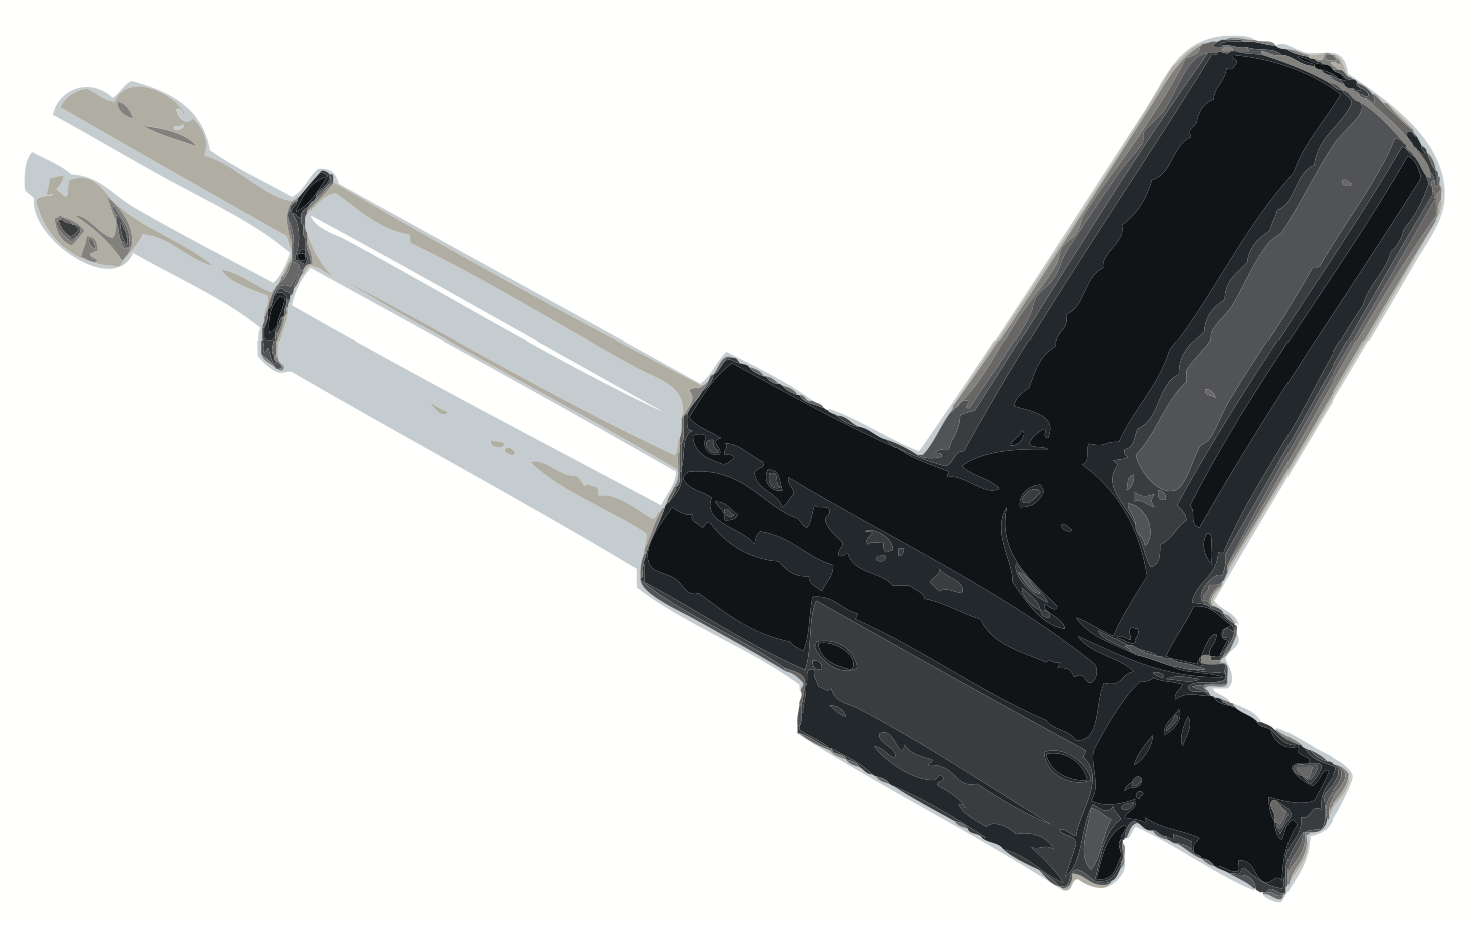
\includegraphics[width=1.6cm]{../fig/actuator_image.png}};
      \node [right of=block4,draw=black, anchor=west,node distance=2.0cm, label=below:{\shortstack[c]{Equations of\\Motion}}, minimum width=2cm, inner sep= 0mm] (block5) {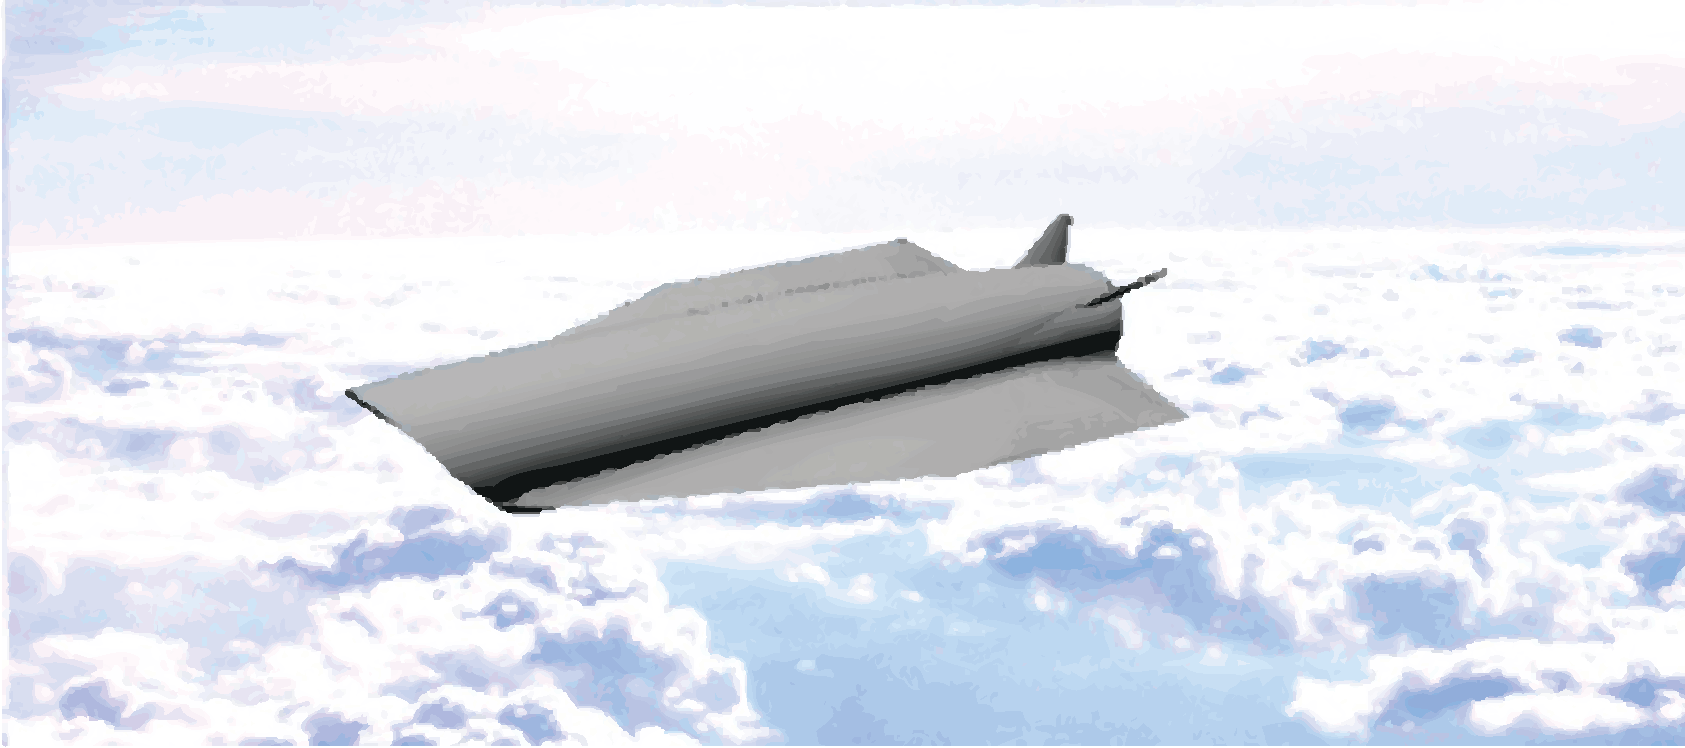
\includegraphics[width=4cm]{../fig/ghvclouds.pdf}};
      \node[whitesum,right of=block5, node distance=3.0cm] (sum2) {};
      \node[squareblock, minimum height=1cm, minimum width=1.0cm, right of=sum2,node distance=1.5cm] (block6) {ZOH};
      \node[squareblock, minimum height=1cm, minimum width=1.0cm, right of=block6,node distance=1.6cm] (block7) {Filter};
      \node[output, right of=block7,node distance=1.5cm] (output1) {};
      \node[input, below of=block2,node distance=1.0cm](input2){};
      \node[input, above of=sum2,node distance=1.0cm](input3){};
      \draw [->] (b1inA) + (-2.5cm,0cm) -> node [pos=0.15]{$z_{\text{cmd}}$}  (b1inA);
      \draw [->] (b1inB) + (-0.5cm,0cm) -> (b1inB);
      \draw [->] (b2inA) + (-1cm,0cm) -> (b2inA);
      \draw [->] (b2inB) + (-2.0cm,0cm) -> node[name=TB,node distance=2.5cm]{} (b2inB);
      \draw[->](block7) --  node[name=yi,pos=0.4]{} (output1);
      \draw[-](yi) |- (input2);
      \draw[-](b1inB) + (-0.5cm,0cm) -- (2B2);
      \draw[-](b1inA) + (-1.0cm,0cm) -- (2A2) ;
      \draw[-] (b2inB) + (-2.0cm,0cm) |- (input2);
      \draw[->](block1) -- (sum1);
      \draw[->](block2) -| (sum1);
      \draw[->](sum1) -- (block3);
      \draw[->](block3) -- (block4);
      \draw[->](block4) -- (block5);
      \draw[->](block5) -- (sum2);
      \draw[->](sum2) -- (block6);
      \draw[->](block6) -- node[name=azoh,pos=0.4]{} (block7);
      \draw[->](input3) -- (sum2);

      \begin{pgfonlayer}{background}
        \path (block1 |- block1)+(-2.5,0.7) node (c) {};
        \path (block2 -| block2)+(2.5,-0.7) node (d) {};
        \path[fill=gray!20, draw, dashed] (c) rectangle (d);
      \end{pgfonlayer}

      \begin{pgfonlayer}{background}
        \path (block6 |- block6)+(-0.7,0.7) node (c) {};
        \path (block7 -| block7)+(0.7,-0.7) node (d) {};
        \path[fill=gray!20, draw, dashed] (c) rectangle (d);
      \end{pgfonlayer}

      % \node [below of=block2, node distance = 0.9cm] {Controller};
      \node [above of=block1, node distance = 0.9cm] {100 Hz};
      \node [above of=azoh, node distance = 0.8cm] {600 Hz};
      \node [above of=sum2, node distance = 1.2cm] {noise};
    \end{tikzpicture}
    \caption{Baseline plus adaptive control block diagram\label{fig.baseplusadaptiveblock}}
  \end{center}
\end{figure}

  \clearpage
\section*{\currfilename}

\begin{figure}[H]
  \begin{center}
    \begin{tikzpicture}[auto, scale=0.85, every node/.style={transform shape}, node distance=1.0cm, >=latex']
      \node[squareblock, minimum height=1cm, minimum width=2cm] (block1){\shortstack[c]{Baseline\\Controller}};
      \node[squareblock, below of=block1, node distance=1.5cm, minimum height=1cm, minimum width=2cm] (block2){\shortstack[c]{Adaptive\\Controller}};
      \matrix[ampersand replacement=\&, row sep=0.5cm, left of=block1,node distance=1cm] (block1in) {
      \node [coordinate] (b1inA) {};\\
      \node [coordinate] (b1inB) {};\\
      };
      \matrix[ampersand replacement=\&, row sep=0.5cm, left of=block2,node distance=1cm] (block2in) {
      \node [coordinate] (b2inA) {};\\
      \node [coordinate] (b2inB) {};\\
      };
      \node [left of=b2inB, node distance=0.5cm] (2B) {};
      \node [below of=2B, node distance=0.12cm] (2B2) {};
      \node [left of=b2inA, node distance=1.0cm] (2A) {};
      \node [below of=2A, node distance=0.12cm] (2A2) {};
      \node[whitesum,right of=block1, node distance=2.5cm] (sum1) {};
      \node[squareblock, minimum height=1cm, minimum width=2cm, right of=sum1,node distance=2.5cm] (block3) {Actuators};
      % \node[squareblock, minimum height=1cm, minimum width=2cm, right of=block3,node distance=3.0cm] (block4) {Plant};
      \node [right of=block3,draw=black, anchor=west,node distance=2.0cm, minimum width=2cm, inner sep= 0mm] (block4) {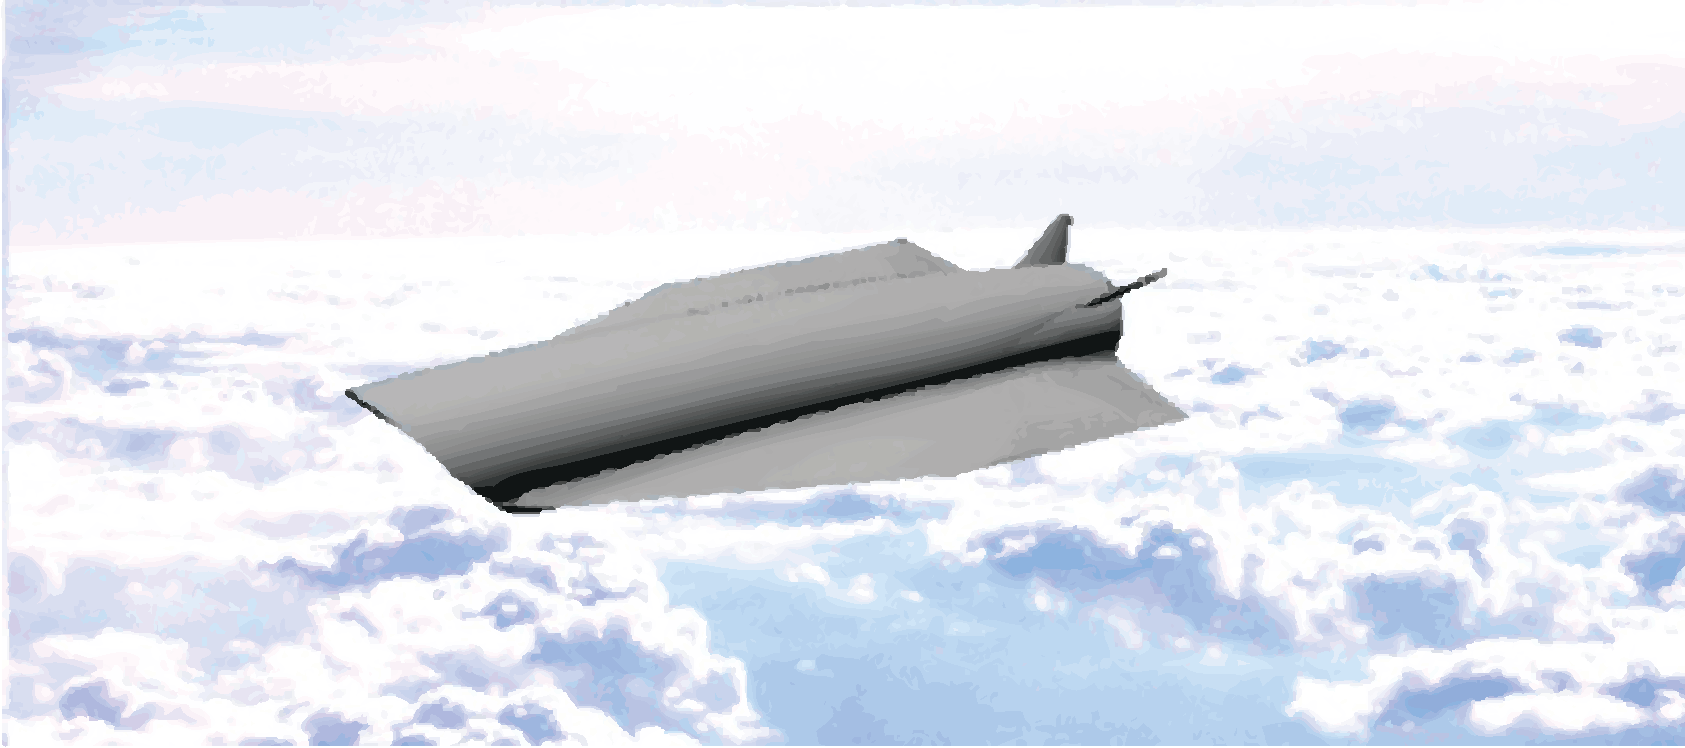
\includegraphics[width=4cm]{../fig/ghvclouds.pdf}};
      \node[squareblock, minimum height=1cm, minimum width=2cm, right of=block4,node distance=4.0cm] (block5) {Sensors};
      \node[output, right of=block5,node distance=2.5cm] (output1) {};
      \node[input, below of=block2,node distance=1.5cm](input2){};
      \draw [->]  (b1inA) + (-2.5cm,0cm) -> node [pos=0.15]{$z_{\text{cmd}}$}  (b1inA);
      \draw [->]  (b1inB) + (-0.5cm,0cm) -> (b1inB);
      \draw [->]  (b2inA) + (-1cm,0cm) -> (b2inA);
      \draw [->]  (b2inB) + (-2.0cm,0cm) -> node[name=TB,node distance=2.5cm]{} (b2inB);
      \draw[->](block5) --  node[name=yi,pos=0.4]{}(output1);
      \draw[-](yi) |- (input2);
      \draw[-](b1inB) + (-0.5cm,0cm) -- (2B2);
      \draw[-](b1inA) + (-1.0cm,0cm) -- (2A2) ;
      \draw[-] (b2inB) + (-2.0cm,0cm) |- (input2);
      \draw[->](block1) -- node[pos=0.22]{$u_{\text{bl}}$} node[pos=0.9]{$+$} (sum1);
      \draw[->](block2) -| node[pos=0.1]{$u_{\text{ad}}$} node[pos=0.9]{$+$} (sum1);
      \draw[->](sum1) -- (block3);
      \draw[->](block3) -- (block4);
      \draw[->](block4) -- (block5);
      \begin{pgfonlayer}{background}
        \path (block1 |- block1)+(-2.5,0.7) node (c) {};
        \path (block2 -| block2)+(3.0,-0.7) node (d) {};
        \path[fill=gray!20, draw, dashed] (c) rectangle (d);
      \end{pgfonlayer}
      \node [below of=block2, node distance = 0.9cm] {Controller};
    \end{tikzpicture}
    \caption{Baseline plus adaptive control block diagram \label{fig.baseplusadaptiveblock}}
  \end{center}
\end{figure}

  \clearpage
\section*{\currfilename}

\begin{figure}[H]
  \fontsize{10pt}{10pt}\selectfont
  \begin{center}
    \begin{tikzpicture}[auto, scale=1.0, every node/.style={transform shape}, node distance=1.0cm, >=latex']
      \node[squareblock, minimum height=1cm, minimum width=2cm] (block1){\shortstack[c]{Baseline\\Controller}};
      \node[squareblock, below of=block1, node distance=1.5cm, minimum height=1cm, minimum width=2cm] (block2){\shortstack[c]{Adaptive\\Controller}};
      \matrix[ampersand replacement=\&, row sep=0.5cm, left of=block1,node distance=1cm] (block1in) {
        \node [coordinate] (b1inA) {}; \\
        \node [coordinate] (b1inB) {}; \\
      };
      \matrix[ampersand replacement=\&, row sep=0.5cm, left of=block2,node distance=1cm] (block2in) {
        \node [coordinate] (b2inA) {}; \\
        \node [coordinate] (b2inB) {}; \\
      };
      \node [left of=b2inB, node distance=0.5cm] (2B) {};
      \node [below of=2B, node distance=0.12cm] (2B2) {};
      \node [left of=b2inA, node distance=1.0cm] (2A) {};
      \node [below of=2A, node distance=0.12cm] (2A2) {};
      \node[whitesum,right of=block1, node distance=2.5cm] (sum1) {};
      \node[squareblock, minimum height=1cm, minimum width=2cm, right of=sum1,node distance=2.5cm] (block3) {Plant};
      \node[squareblock, minimum height=1cm, minimum width=2cm, above of=block3,node distance=1.5cm] (block4) {\shortstack[c]{Reference\\Model}};
      \node[whitesum,right of=block3, node distance=2.5cm] (sum2) {};
      \node[output, right of=sum2,node distance=1.5cm] (output1) {};
      \node[input, below of=block2,node distance=1.0cm](input2){};
      \draw [->]  (b1inA) + (-2.5cm,0cm) -> node [pos=0.15]{$z_{\text{cmd}}$}  (b1inA);
      \draw [->]  (b1inB) + (-0.5cm,0cm) -> (b1inB);
      \draw [->]  (b2inA) + (-1cm,0cm) -> (b2inA);
      \draw [->]  (b2inB) + (-0.5cm,0cm) -> node[name=TB,node distance=2.5cm]{} (b2inB);
      \draw[->](block3) -- node[pos=0.5]{$x$} node[pos=0.9]{$+$} node[name=xi,pos=0.4]{} (sum2);
      \draw[->](sum2) --  node[name=yi,pos=0.4]{} node[pos=0.6]{$e^{o}$} (output1);
      \draw[-](xi) |- (input2);
      \draw[-](b1inB) + (-0.5cm,0cm) -- (2B2);
      \draw[-](b1inA) + (-1.0cm,0cm) -- (2A2) ;
      \draw[-] (b2inB) + (-0.5cm,0cm) |- (input2);
      \draw[->](block1) -- node[pos=0.32]{$u_{\text{bl}}$} node[pos=0.9]{$+$} (sum1);
      \draw[->](block2) -| node[pos=0.2]{$u_{\text{ad}}$} node[pos=0.9]{$+$} (sum1);
      \draw[->](sum1) -- node[pos=0.5]{$u$} (block3);
      \draw[->](block4) -| node[pos=0.2]{$x_{m}^{o}$} node[pos=0.9]{$-$} (sum2);
      \draw [->]  (b1inA) + (-0.5cm,0cm) |- (block4);
    \end{tikzpicture}
    \caption{Classical model-reference adaptive control architecture\label{fig:ormblock}}
  \end{center}
\end{figure}

  \clearpage
\section*{\currfilename}

\begin{figure}[H]
  \fontsize{10pt}{10pt}\selectfont
  \begin{center}
    \begin{tikzpicture}[auto, scale=1.0, every node/.style={transform shape}, node distance=1.0cm, >=latex']
      \node[squareblock, minimum height=1cm, minimum width=2cm] (block1){\shortstack[c]{Baseline\\Controller}};
      \node[squareblock, below of=block1, node distance=1.5cm, minimum height=1cm, minimum width=2cm] (block2){\shortstack[c]{Adaptive\\Controller}};
      \matrix[ampersand replacement=\&, row sep=0.5cm, left of=block1,node distance=1cm] (block1in) {
        \node [coordinate] (b1inA) {}; \\
        \node [coordinate] (b1inB) {}; \\
      };
      \matrix[ampersand replacement=\&, row sep=0.5cm, left of=block2,node distance=1cm] (block2in) {
        \node [coordinate] (b2inA) {}; \\
        \node [coordinate] (b2inB) {}; \\
      };
      \node [left of=b2inB, node distance=0.5cm] (2B) {};
      \node [below of=2B, node distance=0.12cm] (2B2) {};
      \node [left of=b2inA, node distance=1.0cm] (2A) {};
      \node [below of=2A, node distance=0.12cm] (2A2) {};
      \node[whitesum,right of=block1, node distance=2.5cm] (sum1) {};
      \node[squareblock, minimum height=1cm, minimum width=2cm, right of=sum1,node distance=2.5cm] (block3) {Plant};
      \node[squareblock, minimum height=1cm, minimum width=2cm, above of=block3,node distance=1.5cm] (block4) {\shortstack[c]{Reference\\Model}};
      \node [above of=block4, node distance = 1.5cm] (tempnode) {};
      \node[squareblock, minimum height=1cm, minimum width=1cm, right of=tempnode,node distance=1.5cm] (block5) {$L$};
      \node[whitesum,right of=block3, node distance=2.5cm] (sum2) {};
      \node[output, right of=sum2,node distance=2.0cm] (output1) {};
      \node[input, below of=block2,node distance=1.0cm](input2){};
      \draw [->]  (b1inA) + (-2.5cm,0cm) -> node [pos=0.15]{$z_{\text{cmd}}$}  (b1inA);
      \draw [->]  (b1inB) + (-0.5cm,0cm) -> (b1inB);
      \draw [->]  (b2inA) + (-1cm,0cm) -> (b2inA);
      \draw [->]  (b2inB) + (-0.5cm,0cm) -> node[name=TB,node distance=2.5cm]{} (b2inB);
      \draw[->](block3) -- node[pos=0.5]{$x$} node[pos=0.9]{$+$} node[name=xi,pos=0.4]{} (sum2);
      % \draw[->](sum2) --  node[name=yi,pos=0.4]{} node[pos=0.6]{$e^{c}$} (output1);
      \draw[->](sum2) --  node[name=yi,pos=0.4]{} node[pos=0.8]{$e^{c}$} (output1);
      \node [below of=yi, node distance = 0.25cm] (tempnode2) {};
      \draw[-](xi) |- (input2);
      \draw[->](tempnode2) |- (block5);
      \draw[-](b1inB) + (-0.5cm,0cm) -- (2B2);
      \draw[-](b1inA) + (-1.0cm,0cm) -- (2A2) ;
      \draw[-] (b2inB) + (-0.5cm,0cm) |- (input2);
      \draw[->](block1) -- node[pos=0.32]{$u_{\text{bl}}$} node[pos=0.9]{$+$} (sum1);
      \draw[->](block2) -| node[pos=0.2]{$u_{\text{ad}}$} node[pos=0.9]{$+$} (sum1);
      \draw[->](sum1) -- node[pos=0.5]{$u$} (block3);
      \draw[->](block4) -| node[pos=0.2]{$x_{m}^{c}$} node[pos=0.9]{$-$} (sum2);
      \draw [->]  (b1inA) + (-0.5cm,0cm) |- (block4);
      \draw[->](block5) -| (block4);
    \end{tikzpicture}
    \caption{Closed loop reference model adaptive control architecture\label{fig:ormblock}}
  \end{center}
\end{figure}


  \clearpage
\section*{\currfilename}

% We need layers to draw the block diagram
\pgfdeclarelayer{background}
\pgfdeclarelayer{foreground}
\pgfsetlayers{background, main, foreground}

\begin{figure}[H]
  \fontsize{10pt}{10pt}\selectfont
  \begin{center}
    \begin{tikzpicture}[auto, scale=1.0, every node/.style={transform shape}, node distance=1.0cm, >=latex']
      \node[mux, minimum height=2.0cm, minimum width=0.1cm] (block2){};
      \matrix[ampersand replacement=\&, row sep=1.0cm, left of=block2, node distance=0.05cm] (block2in) {
      \node [coordinate] (b2inA) {};\\
      \node [coordinate] (b2inB) {};\\
      };
      \node[squareblock, minimum height=1cm, minimum width=1cm, left of=b2inB, node distance=1.5cm] (block1){$\frac{1}{s}$};
      \node[whitesum, left of=block1, node distance=1.5cm] (sum1) {};
      \node[input, left of=sum1,node distance=2.5cm](input1){};
      \node[squareblock, minimum height=1cm, minimum width=1cm, below of=sum1, node distance=1.5cm] (block3){$C_{pz}$};
      \node[input, right of=block2,node distance=1.0cm](input4a){};
      \node[input, right of=input4a,node distance=1.0cm](input4b){};
      \node[squareblock, minimum height=1cm, minimum width=1cm, above of=input4b,node distance=0.75cm] (block4) {$K_{\text{lqr}}^{\top}$};
      \node[roundblock, minimum height=1cm, minimum width=1cm, below of=input4b,node distance=0.75cm] (block5) {$\theta^{\top}$};
      \node[whitesum, right of=input4b, node distance=2.0cm] (sum2) {};
      \node[squareblock, minimum height=1cm, minimum width=2cm, right of=sum2,node distance=2.5cm] (block6) {Plant};
      \node[input, right of=block3,node distance=2.3cm](input2){};
      \node[squareblock, minimum height=1cm, minimum width=2cm, above of=block6,node distance=1.75cm] (block7) {\shortstack[c]{Reference\\Model}};
      \node[whitesum,right of=block6, node distance=2.5cm] (sum3) {};
      \node[output, right of=sum3,node distance=1.0cm] (output1) {};
      \node[input, right of=input1,node distance=1.0cm](input1a){};
      % \node[output, below of=block5,node distance=1.5cm] (output2) {};
      % Adaptive Arrow
      \coordinate (arrow1) at ([xshift=-0.7cm,yshift=-0.7cm] block5);
      \coordinate (arrow2) at (block5.225);
      \coordinate (arrow3) at (block5.45);
      \coordinate (arrow4) at ([xshift=0.7cm,yshift=0.7cm] block5);
      \draw[-](arrow1) -- (arrow2);
      \draw[->](arrow3) -- (arrow4);
      \node[output, below of=arrow1,node distance=0.2cm] (output2) {};
      % Shaded box
      \begin{pgfonlayer}{background}
      \path (sum1 |- sum1)+(-0.75,2.0) node (c) {};
      \path (sum2 -| sum2)+(0.5,-2.75) node (d) {};
      \path[fill=gray!20, draw, dashed] (c) rectangle (d);
      \end{pgfonlayer}
      % Draw
      \draw[->](input1) -- node[pos=0.2]{$z_{\text{cmd}}$} (sum1);
      \draw[->](sum1) -- node[pos=0.5]{$\dot{x}_{e}$} (block1);
      \draw[->](block1) -- node[pos=0.6]{$x_{e}$} (b2inB);
      \draw[->](block2) -- node[name=x,pos=0.5]{$x$} (input4a);
      \draw[->](input4a) |- (block4);
      \draw[->](input4a) |- (block5);
      \draw[->](block4) -| node[pos=0.2]{$u_{\text{bl}}$} node[pos=0.9]{$+$} (sum2);
      \draw[->](sum2) -- node[pos=0.7]{$u$} (block6);
      \draw[->](block5) -| node[pos=0.2]{$u_{\text{ad}}$} node[pos=0.9]{$+$} (sum2);
      \draw[->](block3) -- node[pos=0.5]{$z$} (sum1);
      \draw[->](input2) -- (block3);
      \draw[->](block6) -- node[pos=0.3]{$x_{p}$} node[name=xp,pos=0.5]{} node[pos=0.8]{$+$} (sum3);
      \draw[->](block7) -| node[pos=0.2]{$x_{m}^{o}$} node[pos=0.9]{$-$} (sum3);
      \draw[-](sum3) -- node[name=eo,pos=0.5]{$e^{o}$} (output1);
      \draw[-](xp) |- node[pos=0.5]{} (input2);
      % \draw[-](output2) -| node[pos=0.5]{} (input2);
      \draw[->](input2) |- node[pos=0.8]{$x_{p}$} (b2inA);
      \draw[->](input1a) |- (block7);
      \draw[-](output1) |- (output2);
      \draw[-](output2) -| (arrow1);
    \end{tikzpicture}
  \end{center}
\end{figure}

  \clearpage
\section*{\currfilename}

\begin{figure}[H]
  \fontsize{10pt}{10pt}\selectfont
  \begin{center}
    \begin{tikzpicture}[auto, scale=1.0, every node/.style={transform shape}, node distance=1.0cm, >=latex']
      \node[mux, minimum height=2.0cm, minimum width=0.1cm] (block2){};

      \matrix[ampersand replacement=\&, row sep=1.0cm, left of=block2, node distance=0.05cm] (block2in) {
        \node [coordinate] (b2inA) {}; \\
        \node [coordinate] (b2inB) {}; \\
      };

      \node[squareblock, minimum height=1cm, minimum width=1cm, left of=b2inB, node distance=1.5cm] (block1){$\frac{1}{s}$};
      \node[whitesum, left of=block1, node distance=1.5cm] (sum1) {};
      \node[input, left of=sum1,node distance=2.5cm](input1){};
      \node[squareblock, minimum height=1cm, minimum width=1cm, below of=sum1, node distance=1.5cm] (block3){$C_{pz}$};
      \node[input, right of=block2,node distance=1.0cm](input4a){};
      \node[input, right of=input4a,node distance=1.0cm](input4b){};
      \node[squareblock, minimum height=1cm, minimum width=1cm, above of=input4b,node distance=0.75cm] (block4) {$K_{\text{lqr}}^{\top}$};
      \node[roundblock, minimum height=1cm, minimum width=1cm, below of=input4b,node distance=0.75cm] (block5) {$\theta^{\top}$};
      \node[whitesum, right of=input4b, node distance=2.0cm] (sum2) {};
      \node[squareblock, minimum height=1cm, minimum width=2cm, right of=sum2,node distance=2.5cm] (block6) {Plant};
      \node[input, right of=block3,node distance=2.3cm](input2){};
      \node[squareblock, minimum height=1cm, minimum width=2cm, above of=block6,node distance=1.75cm] (block7) {\shortstack[c]{Reference\\Model}};
      \node[whitesum,right of=block6, node distance=2.5cm] (sum3) {};
      \node[output, right of=sum3,node distance=1.0cm] (output1) {};
      \node[input, right of=input1,node distance=1.0cm](input1a){};
      % \node[output, below of=block5,node distance=1.5cm] (output2) {};
      % Adaptive Arrow
      \coordinate (arrow1) at ([xshift=-0.7cm,yshift=-0.7cm] block5);
      \coordinate (arrow2) at (block5.225);
      \coordinate (arrow3) at (block5.45);
      \coordinate (arrow4) at ([xshift=0.7cm,yshift=0.7cm] block5);
      \draw[-](arrow1) -- (arrow2);
      \draw[->](arrow3) -- (arrow4);
      \node[output, below of=arrow1,node distance=0.2cm] (output2) {};

      % Shaded box
      \begin{pgfonlayer}{background}
        \path (sum1 |- sum1)+(-0.75,2.0) node (c) {};
        \path (sum2 -| sum2)+(0.5,-2.75) node (d) {};
        \path[fill=gray!20, draw, dashed] (c) rectangle (d);
      \end{pgfonlayer}

      % Draw
      \draw[->](input1) -- node[pos=0.2]{$z_{\text{cmd}}$} (sum1);
      \draw[->](sum1) -- node[pos=0.5]{$\dot{x}_{e}$} (block1);
      \draw[->](block1) -- node[pos=0.6]{$x_{e}$} (b2inB);
      \draw[->](block2) -- node[name=x,pos=0.5]{$x$} (input4a);
      \draw[->](input4a) |- (block4);
      \draw[->](input4a) |- (block5);
      \draw[->](block4) -| node[pos=0.2]{$u_{\text{bl}}$} node[pos=0.9]{$+$} (sum2);
      \draw[->](sum2) -- node[pos=0.7]{$u$} (block6);
      \draw[->](block5) -| node[pos=0.2]{$u_{\text{ad}}$} node[pos=0.9]{$+$} (sum2);
      \draw[->](block3) -- node[pos=0.5]{$z$} (sum1);
      \draw[->](input2) -- (block3);
      \draw[->](block6) -- node[pos=0.3]{$x_{p}$} node[name=xp,pos=0.5]{} node[pos=0.8]{$+$} (sum3);
      \draw[->](block7) -| node[pos=0.2]{$x_{m}^{o}$} node[pos=0.9]{$-$} (sum3);
      \draw[-](sum3) -- node[name=eo,pos=0.5]{$e^{o}$} (output1);
      \draw[-](xp) |- node[pos=0.5]{} (input2);
      % \draw[-](output2) -| node[pos=0.5]{} (input2);
      \draw[->](input2) |- node[pos=0.8]{$x_{p}$} (b2inA);
      \draw[->](input1a) |- (block7);
      \draw[-](output1) |- (output2);
      \draw[-](output2) -| (arrow1);

      % Add L
      \node[squareblock, minimum height=1cm, minimum width=1cm, above of=sum3,node distance=2.5cm] (block8) {$L$};
      \draw[->](output1) |- (block8);
      \draw[->](block8) -| (block7);
    \end{tikzpicture}
  \end{center}
\end{figure}

  \clearpage
\section*{\currfilename}

\begin{figure}[H]
  \begin{center}
    \begin{tikzpicture}[scale=1, auto, node distance=2cm,>=latex']
      \matrix[ampersand replacement=\&, column sep=0.5cm, node distance=2.5cm] (regions) at (0,0){
        \node[block, minimum height=2cm, minimum width=2cm] (R1) {}; \\
      };

      \node [coordinate, above of=R1] (topc) {};
      \node [coordinate, right of=topc, node distance=0.7cm] (topr) {};
      \node [coordinate, left of=topc, node distance=0.7cm] (topl) {};
      \node [coordinate, below of=R1] (botc) {};
      \node [coordinate, right of=botc, node distance=0.7cm] (botr) {};
      \node [coordinate, left of=botc, node distance=0.7cm] (botl) {};

      % Draw
      \draw [<-] (R1.north) -- node [pos=0.5]{} (topc);
      \draw [<-] (R1.north) + (0.7cm,0cm) -- node [pos=0.5]{} (topr);
      \draw [<-] (R1.north) + (-0.7cm,0cm) -- node [pos=0.5]{} (topl);
      \draw [<-] (R1.south) -- node [pos=0.5]{} (botc);
      \draw [<-] (R1.south) + (0.7cm,0cm) -- node [pos=0.5]{} (botr);
      \draw [<-] (R1.south) + (-0.7cm,0cm) -- node [pos=0.5]{} (botl);
    \end{tikzpicture}
  \end{center}
\end{figure}

  \clearpage
\section*{\currfilename}

\begin{figure}[H]
  \fontsize{10pt}{10pt}\selectfont
  \begin{center}
    % \resizebox{8cm}{2.6cm}{
    \begin{tikzpicture}[auto, scale=1.0, every node/.style={transform shape}, node distance=1.0cm, >=latex']
      \node[squareblock, minimum height=1cm, minimum width=2cm] (block1){Baseline};
      \node[squareblock, below of=block1, node distance=1.5cm, minimum height=1cm, minimum width=2cm] (block2){Adaptive};

      \matrix[ampersand replacement=\&, row sep=0.5cm, left of=block1,node distance=1cm] (block1in) {
        \node [coordinate] (b1inA) {}; \\
        \node [coordinate] (b1inB) {}; \\
      };

      \matrix[ampersand replacement=\&, row sep=0.5cm, left of=block2,node distance=1cm] (block2in) {
        \node [coordinate] (b2inA) {}; \\
        \node [coordinate] (b2inB) {}; \\
      };

      \node[whitesum,right of=block1, node distance=2.0cm] (sum1) {};
      \node[squareblock, minimum height=1cm, minimum width=2cm, right of=sum1,node distance=2.5cm] (block3) {Plant};
      \node[squareblock, minimum height=1cm, minimum width=2cm, above of=block3,node distance=1.75cm] (block4) {\shortstack[c]{Reference\\Model}};
      \node[whitesum,right of=block3, node distance=2.5cm] (sum2) {};
      \node[input,below of=block2, node distance=1.5cm] (input2) {};
      \node[output,right of=sum2, node distance=1.5cm] (output1) {};

      % Gray shaded box
      \begin{pgfonlayer}{background}
      \path (block1 |- block1)+(-2.5,0.7) node (c) {};
      \path (block2 -| block2)+(2.5,-0.7) node (d) {};
      \path[fill=gray!20, draw, dashed] (c) rectangle (d);
      \end{pgfonlayer}

      % Draw
      \draw [->]  (b1inA) + (-2.5cm,0cm) -> node [pos=0.0]{$z_{\text{cmd}}$}  (b1inA);
      \draw [->]  (b1inA) + (-2.0cm,0cm) |- node [pos=0.15]{}  (block4);
      \draw [->]  (b1inB) + (-0.5cm,0cm) -> (b1inB);
      \draw [->]  (b2inA) + (-1cm,0cm) -> (b2inA);
      \draw [->]  (b2inB) + (-2.0cm,0cm) -> (b2inB);
      \draw [-]  (b2inB) + (-2.0cm,0cm) |- (input2);
      \draw[->](block3) --  node[name=yi,pos=0.5]{} (sum2);
      \draw[-](yi) |- (input2);
      % \draw[-](b1inB) + (-0.5cm,0cm) -- (2B2);
      % \draw[-](b1inA) + (-1.0cm,0cm) -- (2A2) ;
      \draw[->](block1) -- (sum1);
      \draw[->](block2) -| (sum1);
      \draw[->](sum1) -- (block3);
      % \draw[->](input1a) + (-2.5cm,0cm) |- (block4);
      \draw[->](block4) -| (sum2);
      \draw[->](sum2) -- (output1);

      % \draw[->](block3) -- (block4);
      % \draw[->](block4) -- (block5);
      % \draw[->](block5) -- (sum2);
      % \draw[->](sum2) -- (block6);
      % \draw[->](block6) -- node[name=azoh,pos=0.4]{} (block7);
      % \draw[->](input3) -- (sum2);
      % \draw[->](input1) -- node[pos=0.2]{$z_{\text{cmd}}$} (sum1);
      % \draw[->](sum1) -- node[pos=0.5]{$\dot{x}_{e}$} (block1);
      % \draw[->](block1) -- node[pos=0.6]{$x_{e}$} (b2inB);
      % \draw[->](block2) -- node[name=x,pos=0.5]{$x$} (input4a);
      % \draw[->](input4a) |- (block4);
      % \draw[->](input4a) |- (block5);
      % \draw[->](block4) -| node[pos=0.2]{$u_{\text{bl}}$} node[pos=0.9]{$+$} (sum2);
      % \draw[->](sum2) -- node[pos=0.7]{$u$} (block6);
      % \draw[->](block5) -| node[pos=0.2]{$u_{\text{ad}}$} node[pos=0.9]{$+$} (sum2);
      % \draw[->](block3) -- node[pos=0.5]{$z$} (sum1);
      % \draw[->](input2) -- (block3);
      % \draw[->](block6) -- node[pos=0.3]{$x_{p}$} node[name=xp,pos=0.5]{} node[pos=0.8]{$+$} (sum3);
      % \draw[->](block7) -| node[pos=0.2]{$x_{m}^{o}$} node[pos=0.9]{$-$} (sum3);
      % \draw[-](sum3) -- node[name=eo,pos=0.5]{$e^{o}$} (output1);
      % \draw[-](xp) |- node[pos=0.5]{} (input2);
      % \draw[->](input2) |- node[pos=0.8]{$x_{p}$} (b2inA);
      % \draw[->](input1a) |- (block7);
      % \draw[-](output1) |- (arrow1);
    \end{tikzpicture}
    % \vspace{-0.1in}
    \caption{\fontsize{7pt}{7pt}\selectfont \textbf{Classical open loop reference model adaptive control architecture}}
  \end{center}
\end{figure}

  \clearpage
\section*{\currfilename}

\begin{figure}[H]
  \fontsize{10pt}{10pt}\selectfont
  \begin{center}
    % \resizebox{8cm}{2.6cm}{
    \begin{tikzpicture}[auto, scale=1.0, every node/.style={transform shape}, node distance=1.0cm, >=latex']
      \node[squareblock, minimum height=1cm, minimum width=2cm] (block1){Baseline};
      \node[squareblock, below of=block1, node distance=1.5cm, minimum height=1cm, minimum width=2cm] (block2){Adaptive};
      \matrix[ampersand replacement=\&, row sep=0.5cm, left of=block1,node distance=1cm] (block1in) {
        \node [coordinate] (b1inA) {}; \\
        \node [coordinate] (b1inB) {}; \\
      };
      \matrix[ampersand replacement=\&, row sep=0.5cm, left of=block2,node distance=1cm] (block2in) {
        \node [coordinate] (b2inA) {}; \\
        \node [coordinate] (b2inB) {}; \\
      };
      \node[whitesum,right of=block1, node distance=2.0cm] (sum1) {};
      %\node[squareblock, minimum height=1cm, minimum width=2cm, right of=sum1,node distance=2.5cm] (block3) {Plant};
      \node [right of=sum1,draw=black, node distance=3.5cm, label=below:{\shortstack[c]{Equations of\\Motion}}, minimum width=2cm, inner sep= 0mm] (block3) {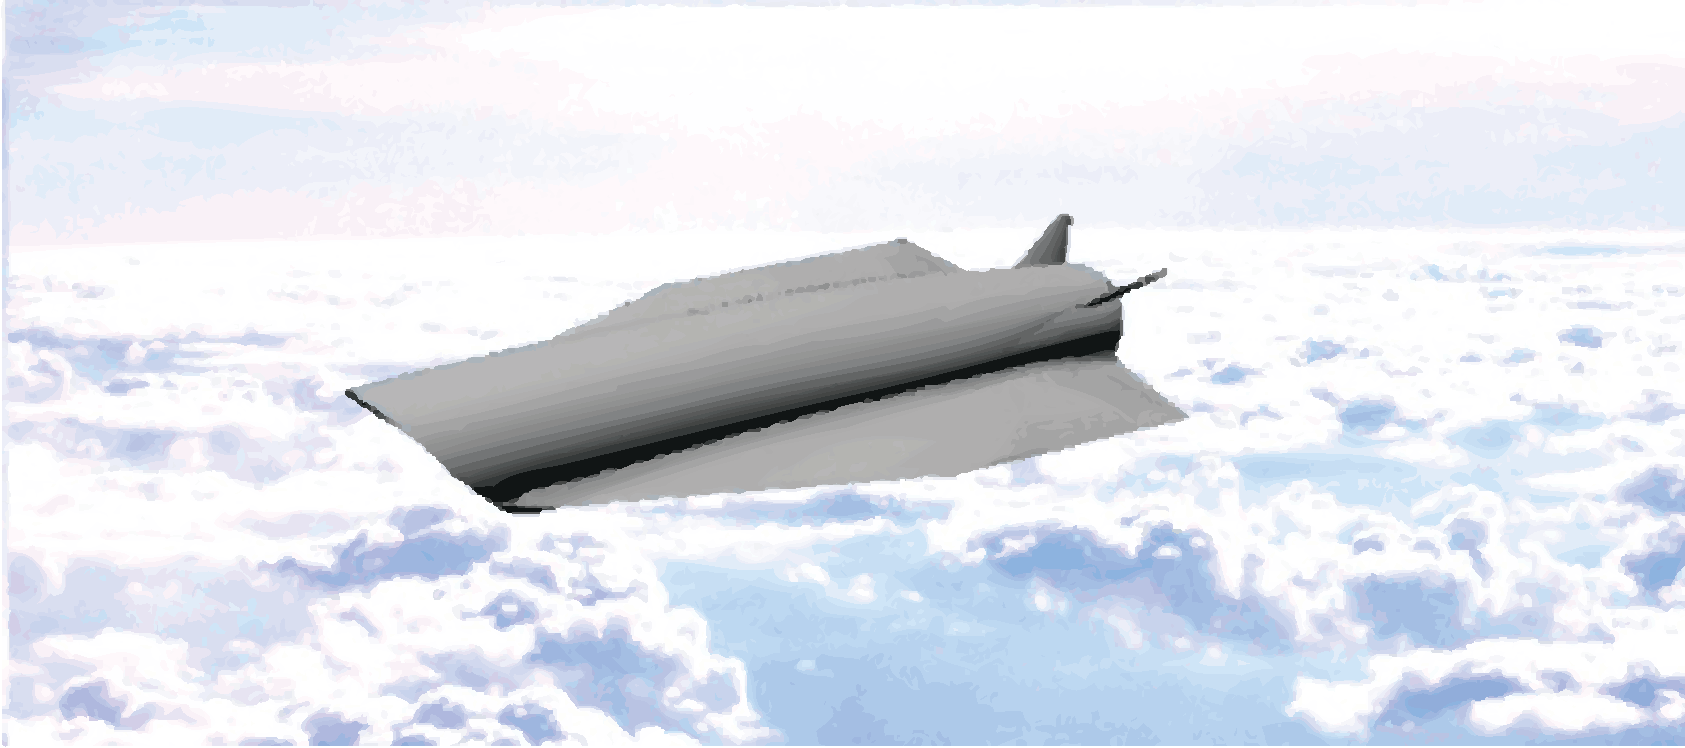
\includegraphics[width=4cm]{../fig/ghvclouds.pdf}};
      \node[squareblock, minimum height=1cm, minimum width=2cm, above of=block3,node distance=1.75cm] (block4) {\shortstack[c]{Reference\\Model}};
      \node[whitesum,right of=block3, node distance=3.5cm] (sum2) {};
      \node[input,below of=block2, node distance=1.5cm] (input2) {};
      \node[output,right of=sum2, node distance=1.5cm] (output1) {};

      % Gray shaded box
      \begin{pgfonlayer}{background}
        \path (block1 |- block1)+(-2.5,0.7) node (c) {};
        \path (block2 -| block2)+(2.5,-0.7) node (d) {};
        \path[fill=gray!20, draw, dashed] (c) rectangle (d);
      \end{pgfonlayer}

      % Draw
      \draw [->] (b1inA) + (-2.5cm,0cm) -> node [pos=0.0]{$z_{\text{cmd}}$}  (b1inA);
      \draw [->] (b1inA) + (-2.0cm,0cm) |- node [pos=0.15]{}  (block4);
      \draw [->] (b1inB) + (-0.5cm,0cm) -> (b1inB);
      \draw [->] (b2inA) + (-1cm,0cm) -> (b2inA);
      \draw [->] (b2inB) + (-2.0cm,0cm) -> (b2inB);
      \draw [-]  (b2inB) + (-2.0cm,0cm) |- (input2);
      \draw[->](block3) --  node[name=yi,pos=0.3]{$x_{p}$} node[pos=0.9]{$+$} (sum2);
      \draw[-](yi) |- (input2);
      % \draw[-](b1inB) + (-0.5cm,0cm) -- (2B2);
      % \draw[-](b1inA) + (-1.0cm,0cm) -- (2A2);
      \draw[->](block1) -- node[pos=0.7]{$+$} (sum1);
      \draw[->](block2) -| node[pos=0.9]{$+$} (sum1);
      \draw[->](sum1) -- node[pos=0.6]{$u$} (block3);
      \draw[->](block4) -| node[pos=0.1]{$x_{m}^{o}$} node[pos=0.95]{$-$} (sum2);
      \draw[->](sum2) -- node[pos=0.4]{$e^{o}$} (output1);
    \end{tikzpicture}
    \caption{\fontsize{7pt}{7pt}\selectfont \textbf{Classical open loop reference model adaptive control architecture}}
  \end{center}
\end{figure}

  \clearpage
\section*{\currfilename}

\begin{figure}[H]
  \fontsize{10pt}{10pt}\selectfont
  \begin{center}
    %\resizebox{8cm}{2.6cm}{
    \begin{tikzpicture}[auto, scale=1.0, every node/.style={transform shape}, node distance=1.0cm, >=latex']
      \node[squareblock, minimum height=1cm, minimum width=2cm] (block1){Baseline};
      \node[squareblock, below of=block1, node distance=1.5cm, minimum height=1cm, minimum width=2cm] (block2){Adaptive};
      \matrix[ampersand replacement=\&, row sep=0.5cm, left of=block1,node distance=1cm] (block1in) {
        \node [coordinate] (b1inA) {}; \\
        \node [coordinate] (b1inB) {}; \\
      };
      \matrix[ampersand replacement=\&, row sep=0.5cm, left of=block2,node distance=1cm] (block2in) {
        \node [coordinate] (b2inA) {}; \\
        \node [coordinate] (b2inB) {}; \\
      };
      \node[whitesum,right of=block1, node distance=2.0cm] (sum1) {};
      %\node[squareblock, minimum height=1cm, minimum width=2cm, right of=sum1,node distance=2.5cm] (block3) {Plant};
      \node [right of=sum1,draw=black, node distance=3.5cm, label=below:{\shortstack[c]{Equations of\\Motion}}, minimum width=2cm, inner sep= 0mm] (block3) {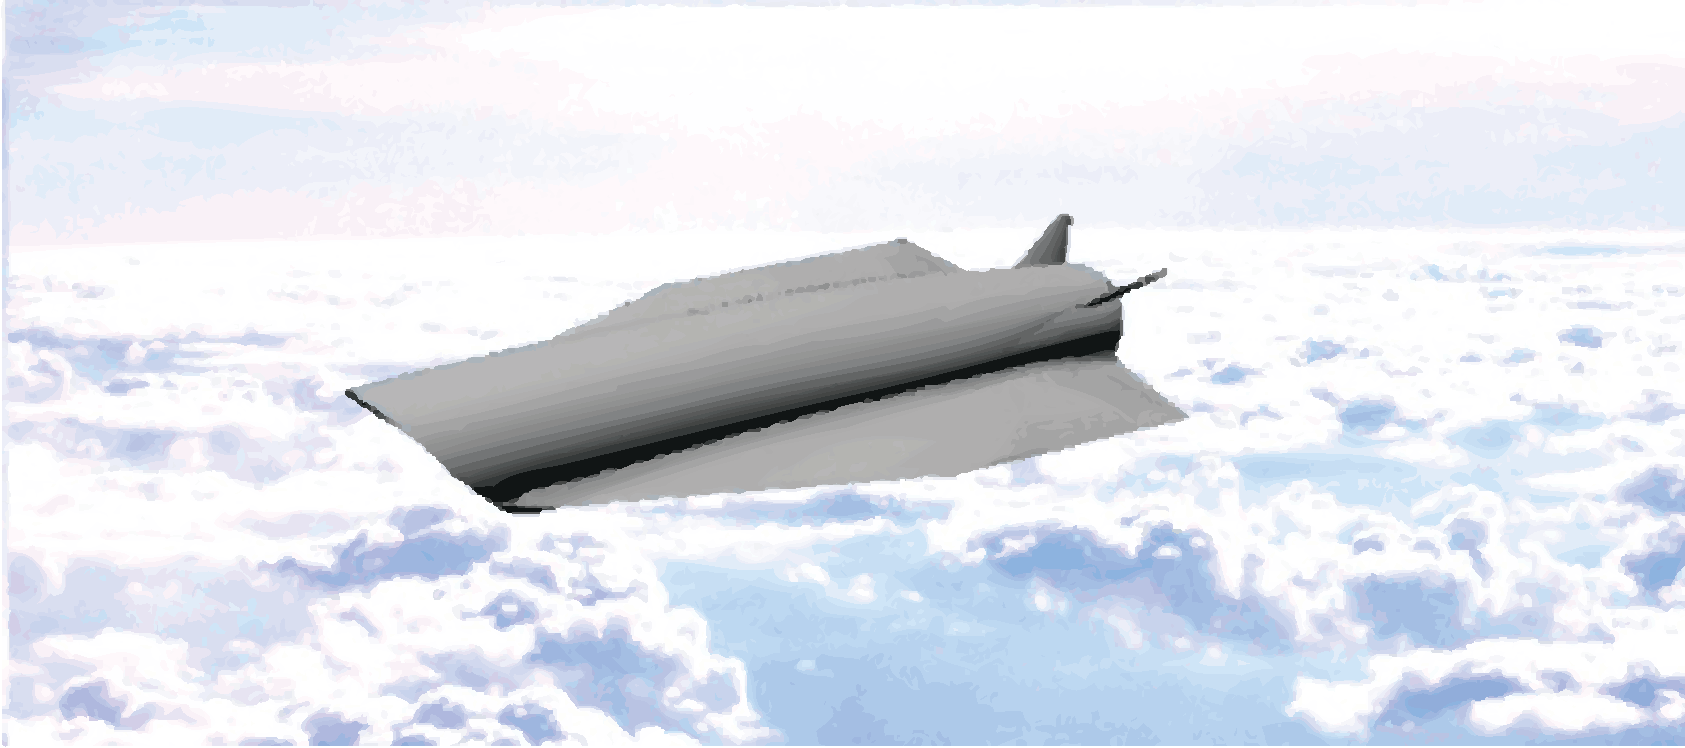
\includegraphics[width=4cm]{../fig/ghvclouds.pdf}};
      \node[squareblock, minimum height=1cm, minimum width=2cm, above of=block3,node distance=1.75cm] (block4) {\shortstack[c]{Reference\\Model}};
      \node[whitesum,right of=block3, node distance=3.5cm] (sum2) {};
      \node[input,below of=block2, node distance=1.5cm] (input2) {};
      \node[output,right of=sum2, node distance=2.5cm] (output1) {};
      \node[squareblock, minimum height=1cm, minimum width=1cm, above of=sum2,node distance=2.75cm] (block5) {$L$};

      % gray shaded box
      \begin{pgfonlayer}{background}
        \path (block1 |- block1)+(-2.5,0.7) node (c) {};
        \path (block2 -| block2)+(2.5,-0.7) node (d) {};
        \path[fill=gray!20, draw, dashed] (c) rectangle (d);
      \end{pgfonlayer}

      % Draw
      \draw [->] (b1inA) + (-2.5cm,0cm) -> node [pos=0.0]{$z_{\text{cmd}}$}  (b1inA);
      \draw [->] (b1inA) + (-2.0cm,0cm) |- node [pos=0.15]{}  (block4);
      \draw [->] (b1inB) + (-0.5cm,0cm) -> (b1inB);
      \draw [->] (b2inA) + (-1cm,0cm) -> (b2inA);
      \draw [->] (b2inB) + (-2.0cm,0cm) -> (b2inB);
      \draw [-]  (b2inB) + (-2.0cm,0cm) |- (input2);
      \draw[->](block3) --  node[name=yi,pos=0.3]{$x$} node[pos=0.9]{$+$} (sum2);
      \draw[-](yi) |- (input2);
      \node [coordinate, left of=b1inB, node distance=0.5cm] (b1inBleft) {};
      \node [coordinate, left of=b2inA, node distance=1.0cm] (b2inAleft) {};
      \draw [-]  (b1inBleft) + (0.0cm,-1.5cm) -- (b1inBleft);
      \draw [-]  (b2inAleft) + (0.0cm,1.5cm) -- (b2inAleft);
      \draw[->](block1) -- node[pos=0.7]{$+$} (sum1);
      \draw[->](block2) -| node[pos=0.9]{$+$} (sum1);
      \draw[->](sum1) -- node[pos=0.6]{$u$} (block3);
      \draw[->](block4) -| node[pos=0.1]{$x_{m}$} node[pos=0.95]{$-$} (sum2);
      \draw[->](sum2) -- node[name=ec,pos=0.3]{} node[pos=0.7]{$e$} (output1);
      \draw[->](ec) + (0cm,-0.1cm) |- (block5);
      \draw[->](block5) -| (block4);
    \end{tikzpicture}
    \caption{\fontsize{7pt}{7pt}\selectfont \textbf{Closed-loop reference model adaptive control architecture}}
  \end{center}
\end{figure}

  \clearpage
\section*{\currfilename}

\begin{figure}[H]
  \fontsize{10pt}{10pt}\selectfont
  \begin{center}
    \resizebox{3.0in}{1.0in}{
    \begin{tikzpicture}[auto, scale=1.0, every node/.style={transform shape}, node distance=1.0cm, >=latex']
      \node[squareblock, minimum height=1cm, minimum width=2cm] (block1){Baseline};
      \node[squareblock, below of=block1, node distance=1.5cm, minimum height=1cm, minimum width=2cm] (block2){Adaptive};

      \matrix[ampersand replacement=\&, row sep=0.5cm, left of=block1,node distance=1cm] (block1in) {
        \node [coordinate] (b1inA) {}; \\
        \node [coordinate] (b1inB) {}; \\
      };

      \matrix[ampersand replacement=\&, row sep=0.5cm, left of=block2,node distance=1cm] (block2in) {
        \node [coordinate] (b2inA) {}; \\
        \node [coordinate] (b2inB) {}; \\
      };

      \node[whitesum,right of=block1, node distance=2.0cm] (sum1) {};
      \node [right of=sum1,draw=black, node distance=3.5cm, label=below:{\shortstack[c]{Equations of\\Motion}}, minimum width=2cm, inner sep= 0mm] (block3) {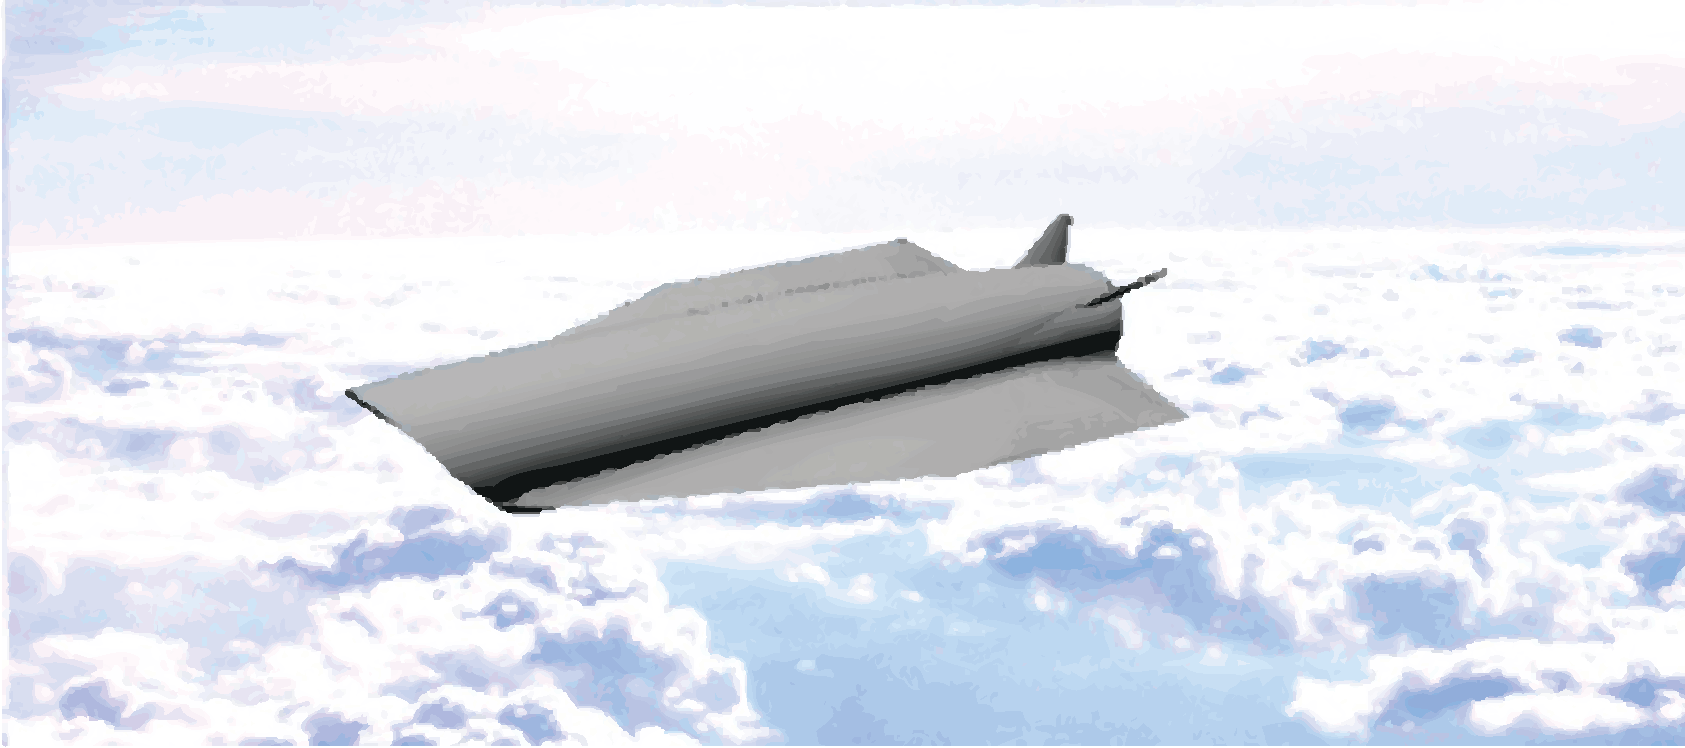
\includegraphics[width=4cm]{../fig/ghvclouds.pdf}};
      \node[squareblock, minimum height=1cm, minimum width=2cm, above of=block3,node distance=1.75cm] (block4) {\shortstack[c]{Reference\\Model}};
      \node[whitesum,right of=block3, node distance=3.5cm] (sum2) {};
      \node[input,below of=block2, node distance=1.5cm] (input2) {};
      \node[output,right of=sum2, node distance=1.5cm] (output1) {};

      % Gray shaded box
      \begin{pgfonlayer}{background}
        \path (block1 |- block1)+(-2.5,0.7) node (c) {};
        \path (block2 -| block2)+(2.5,-0.7) node (d) {};
        \path[fill=gray!20, draw, dashed] (c) rectangle (d);
      \end{pgfonlayer}

      % Draw
      \draw [->]  (b1inA) + (-2.5cm,0cm) -> node [pos=0.0]{$z_{\text{cmd}}$}  (b1inA);
      \draw [->]  (b1inA) + (-2.0cm,0cm) |- node [pos=0.15]{}  (block4);
      \draw [->]  (b1inB) + (-0.5cm,0cm) -> (b1inB);
      \draw [->]  (b2inA) + (-1cm,0cm) -> (b2inA);
      \draw [->]  (b2inB) + (-2.0cm,0cm) -> (b2inB);
      \draw [-]  (b2inB) + (-2.0cm,0cm) |- (input2);
      \draw[->](block3) --  node[name=yi,pos=0.3]{$x_{p}$} node[pos=0.9]{$+$} (sum2);
      \draw[-](yi) |- (input2);
      \node [coordinate, left of=b1inB, node distance=0.5cm] (b1inBleft) {};
      \node [coordinate, left of=b2inA, node distance=1.0cm] (b2inAleft) {};
      \draw [-]  (b1inBleft) + (0.0cm,-1.5cm) -- (b1inBleft);
      \draw [-]  (b2inAleft) + (0.0cm,1.5cm) -- (b2inAleft);
      \draw[->](block1) -- node[pos=0.7]{$+$} (sum1);
      \draw[->](block2) -| node[pos=0.9]{$+$} (sum1);
      \draw[->](sum1) -- node[pos=0.6]{$u$} (block3);
      \draw[->](block4) -| node[pos=0.1]{$x_{m}^{o}$} node[pos=0.95]{$-$} (sum2);
      \draw[->](sum2) -- node[pos=0.4]{$e^{o}$} (output1);
    \end{tikzpicture}}
    \caption{\fontsize{7pt}{7pt}\selectfont \textbf{Classical open loop reference model adaptive control architecture}}
  \end{center}
\end{figure}

  \clearpage
\section*{\currfilename}

\begin{figure}[H]
  \fontsize{10pt}{10pt}\selectfont
  \begin{center}
    %\resizebox{3.0in}{1.0in}{
    \begin{tikzpicture}[auto, scale=1.0, every node/.style={transform shape}, node distance=0.6cm,>=latex']
      \matrix[ampersand replacement=\&, row sep=0cm, node distance=4.0cm] (regions) at (0,0) {
      \node [draw=black, label=below:{\shortstack[c]{GHV Equations\\ of Motion}}, label=above:{$A,B\Lambda,C$},  minimum width=3cm, inner sep=0mm] (block3){\centering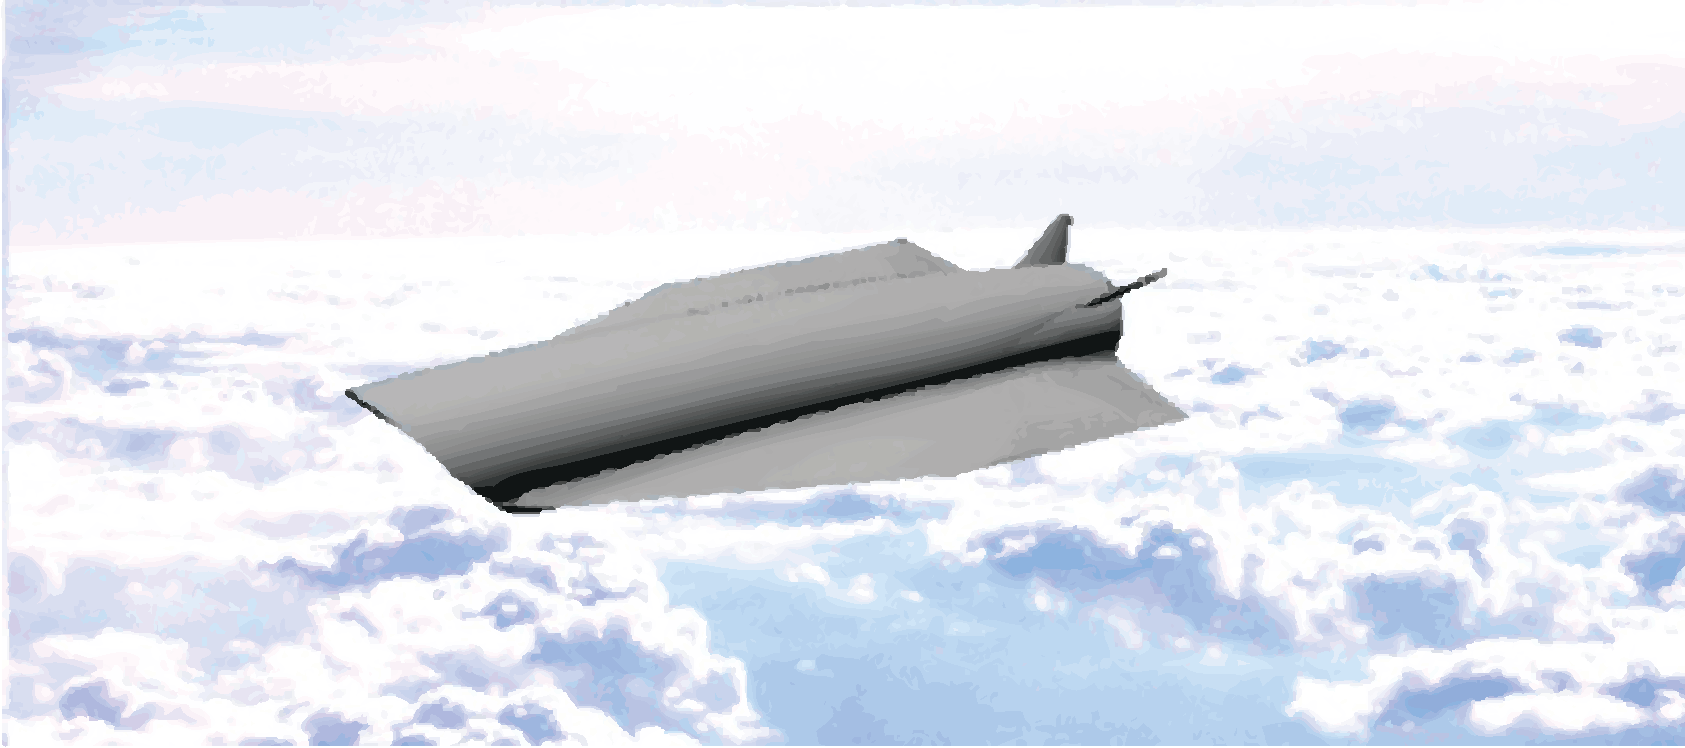
\includegraphics[width=4cm]{../fig/ghvclouds.pdf}}; \\
      };
      %\matrix[ampersand replacement=\&, row sep=0.6cm, left of=block3, node distance=5.0cm] (xxxx) {
      %\node [squareblock, minimum width=2cm] (block1) {Baseline};\\
      %%\node [block, minimum width=2cm] (block2) {\shortstack{Adaptive \\ Augmentation}};\\
      %};
      \node[block,left of=block1, node distance=4.0cm](node1) {};
      %\node [squareblock, minimum width=2cm] (block2) {\shortstack{Adaptive \\ Augmentation}};
      %\draw [<-] (block3.west) + (0cm,0.6cm) -- (block1);
      %\draw [<-] (block3.west) + (0cm,-0.6cm) -- (block2);
      %
      %\draw [->] (R1.east) + (0cm,-0.5cm) -- node [block,pos=0.95]{$y$} (output2);
      %\node[input, below of=block2,node distance=1.5cm](input4){};
      %draw
      %\draw [<-] (block2.west) + (0cm,0.3cm) -- node [block]{test} (block1);

      %\draw [<-] (block2.west) + (0cm,0.3cm) -- node [near end]{$z_{\text{cmd}}$} (b2out1);
      %\draw [<-] (block2.west) + (0cm,-0.3cm) -- node [near end]{$y$} (b2out2);
      %\draw [->] (R1outx) -- node [pos=0.9]{} (output1);
      %\draw [->] (block2) -- node [near start]{$u$} (R1);
      %\draw [->] (input2) -- node [near start]{bias} (R1outx);
      %\draw [->] (R1.east) + (0cm,0.5cm) -- (R1outx);
      %\draw [->] (R1outx) -- node [pos=0.9]{} (output1);
      %\draw [->] (R1.east) + (0cm,-0.5cm) -- node [pos=0.95]{$y$} (output2);
      %\draw [->] (input4) -- node [near start]{$S_{1}$, $L$} (block2);
      %cross out
      %\coordinate (arrow1) at ([xshift=-0.4cm,yshift=-0.3cm] output1);
      %\coordinate (arrow2) at ([xshift=0.2cm,yshift=0.3cm] output1);
      %\coordinate (arrow3) at ([xshift=-0.4cm,yshift=0.3cm] output1);
      %\coordinate (arrow4) at ([xshift=0.2cm,yshift=-0.3cm] output1);
      %\draw[-,red,line width=2](arrow1) -- (arrow2);
      %\draw[-,red,line width=2](arrow3) -- (arrow4);
    \end{tikzpicture}
    %}
  \end{center}
\end{figure}


  \clearpage
\section*{\currfilename}

\pgfdeclarelayer{background}
\pgfdeclarelayer{foreground}
\pgfsetlayers{background,main,foreground}

% Define a few styles and constants
\tikzstyle{sensor}=[draw, fill=blue!20, text width=5em, text centered, minimum height=2.5em]
\tikzstyle{ann} = [above, text width=5em]
\tikzstyle{naveqs} = [sensor, text width=6em, fill=red!20, minimum height=12em, rounded corners]

\def\blockdist{4.5}
\def\edgedist{2.5}

\begin{tikzpicture}
  \node (block3) [squareblock, label=below:{\shortstack[c]{\bf Nonlinear Equations\\ \bf of Motion}}, minimum width=6cm, inner sep=0mm] {\centering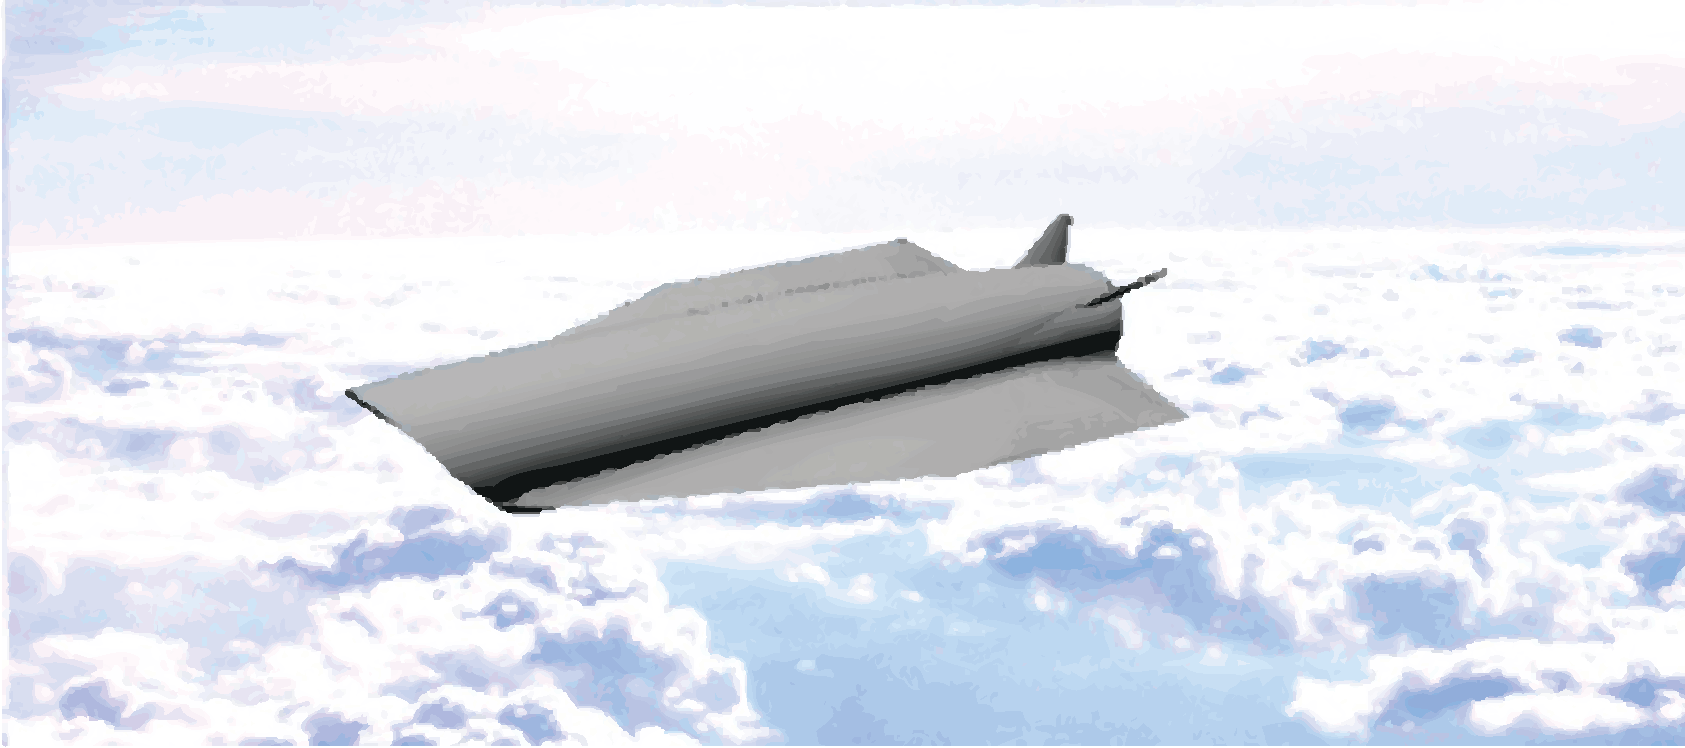
\includegraphics[width=6cm]{../fig/ghvclouds.pdf}};
  \node (naveq) [naveqs] {Navigation equations};
  \path (naveq.145)+(-\blockdist,0) node (block1) [squareblock, minimum width=2.5cm] {Baseline};
  \path (naveq.-145)+(-\blockdist,0) node (block2) [squareblock, minimum width=2.5cm] {\shortstack{Adaptive \\ Augmentation}};
  \node (sum1) [whitesum, right of=block3, node distance=4.5cm] {};
  \node (input1) [input, above of=sum1, node distance=1.5cm] {};
  \node (output1) [input, right of=sum1, node distance=1.5cm] {};
  \path [draw, ->] (block1) -- (block3.west |- block1) ;
  \path [draw, ->] (block2) -- (block3.west |- block2);
  %\path [draw, ->] (block3) -- node[pos=0.7]{$-$} (sum1);
  %\path [draw, ->] (input1) -- node[pos=0.2]{target} node[pos=0.7]{$+$} (sum1);
  %\path [draw, ->] (sum1) -- node[pos=0.7]{error} (output1);
  \draw[->](block3) -- node[pos=0.7, anchor=north]{$-$} (sum1);
  \draw[->](input1) -- node[pos=0.2, anchor=west]{target} node[pos=0.7, anchor=west]{$+$} (sum1);
  \draw[->](sum1) -- node[pos=0.7, anchor=south]{error} (output1);
\end{tikzpicture}

  \clearpage
\section*{\currfilename}

\pgfdeclarelayer{background}
\pgfdeclarelayer{foreground}
\pgfsetlayers{background,main,foreground}
% Define a few styles and constants
\tikzstyle{sensor}=[draw, fill=blue!20, text width=5em, text centered, minimum height=2.5em]
\tikzstyle{ann} = [above, text width=5em]
\tikzstyle{naveqs} = [sensor, text width=6em, fill=red!20, minimum height=12em, rounded corners]
\def\blockdist{4.5}
\def\edgedist{2.5}

\begin{tikzpicture}
  \node (block3) [squareblock, label=below:{\shortstack[c]{\bf Nonlinear Equations\\ \bf of Motion}}, minimum width=6cm, inner sep=0mm] {\centering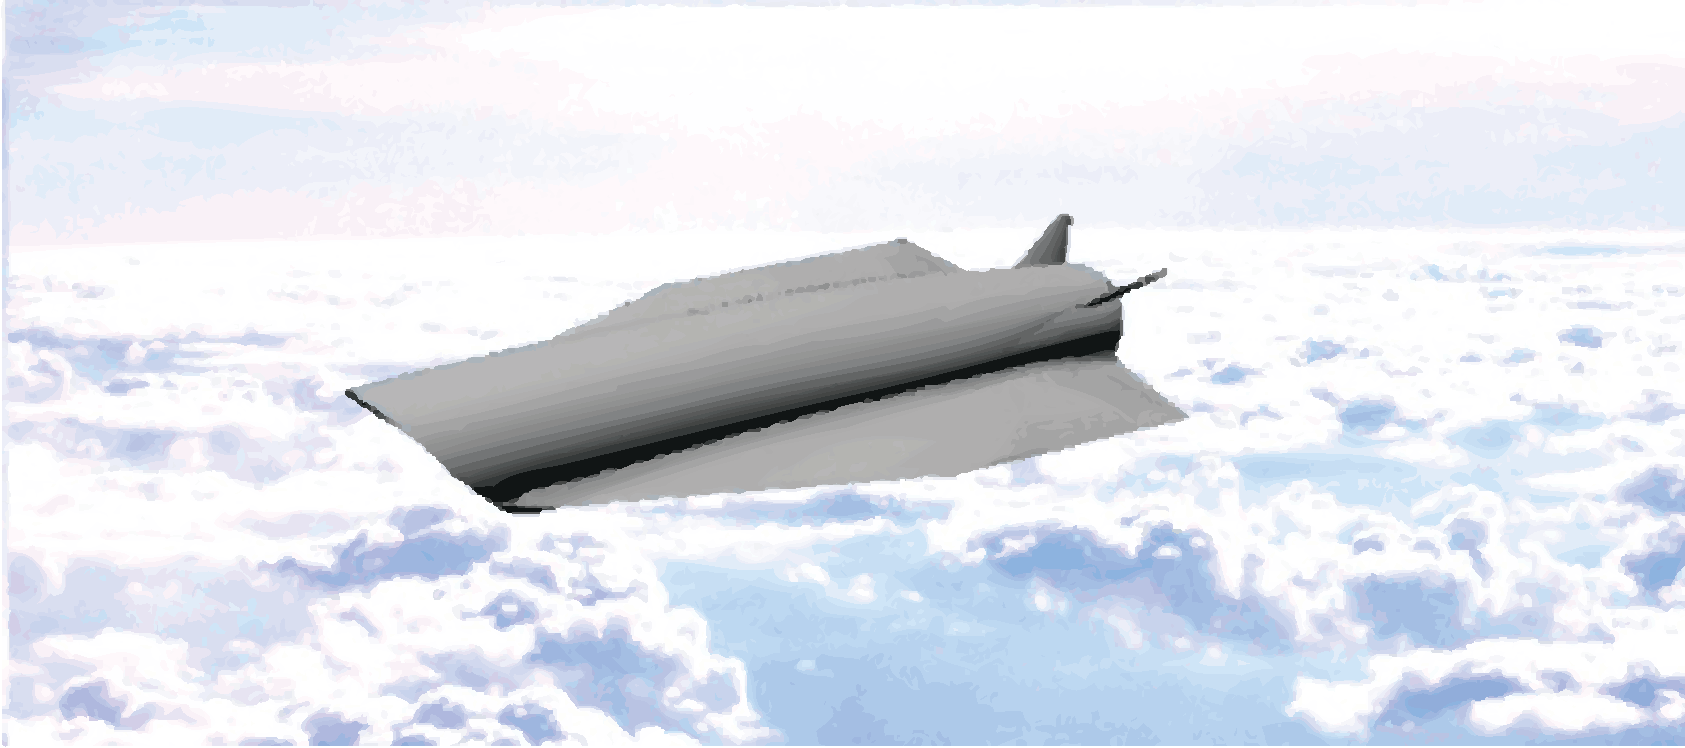
\includegraphics[width=6cm]{../fig/ghvclouds.pdf}};
  \path (naveq.145)+(-\blockdist,0) node (block1) [squareblock, minimum width=2.5cm] {Baseline};
  \path (naveq.-145)+(-\blockdist,0) node (block2) [squareblock, minimum width=2.5cm] {\shortstack{Adaptive \\ Augmentation}};
  \node[squareblock, minimum height=1cm, minimum width=2cm, right of=block3, node distance=5.0cm] (block4) {\shortstack[c]{Error \\ Generator}};
  \node[output, right of=block4,node distance=2.0cm] (output1) {};
  \path [draw, ->] (block1) -- (block3.west |- block1) ;
  \path [draw, ->] (block2) -- (block3.west |- block2);
  \draw[->](block3) -- (block4);
  \draw[->](block4) --  node[above,pos=0.8]{$e$}(output1);
\end{tikzpicture}

  \clearpage
\section*{\currfilename}

\pgfdeclarelayer{background}
\pgfdeclarelayer{foreground}
\pgfsetlayers{background,main,foreground}

% Define a few styles and constants
\tikzstyle{sensor}=[draw, fill=blue!20, text width=5em, text centered, minimum height=2.5em]
\tikzstyle{ann} = [above, text width=5em]
\tikzstyle{naveqs} = [sensor, text width=6em, fill=red!20, minimum height=12em, rounded corners]
\def\blockdist{4.5}
\def\edgedist{2.5}

\begin{tikzpicture}
  \node (block3) [squareblock, label=below:{\shortstack[c]{\bf Nonlinear Equations\\ \bf of Motion}}, minimum width=6cm, inner sep=0mm] {\centering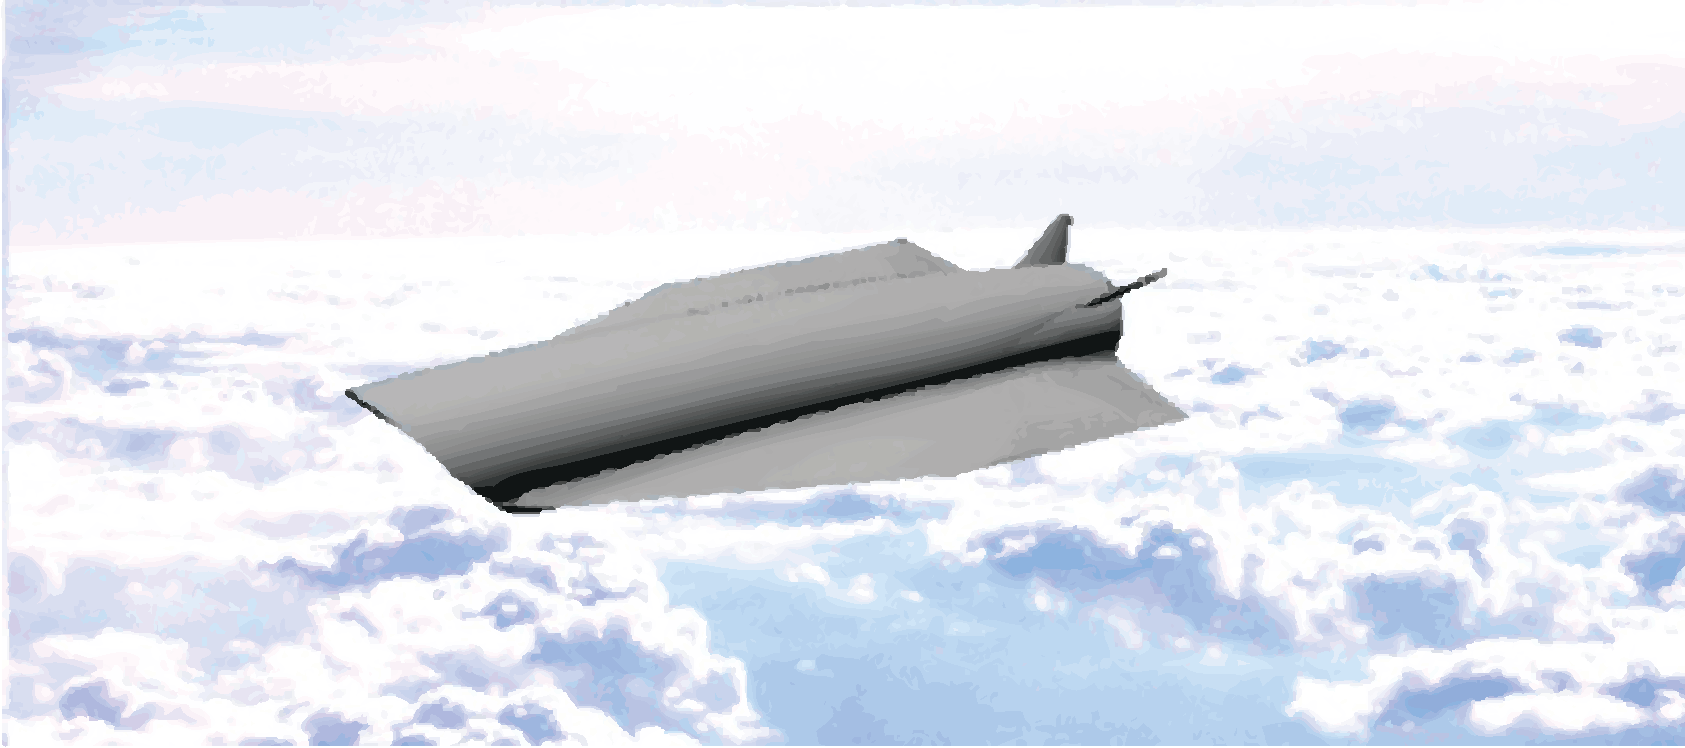
\includegraphics[width=6cm]{../fig/ghvclouds.pdf}};
  \path (naveq.145)+(-\blockdist,0) node (block1) [squareblock, minimum width=2.5cm] {Baseline};
  %\path (naveq.-145)+(-\blockdist,0) node (block2) [squareblock, minimum width=2.5cm] {\shortstack{Adaptive \\ Augmentation}};
  %\node[squareblock, minimum height=1cm, minimum width=2cm, right of=block3, node distance=5.0cm] (block4) {\shortstack[c]{Error \\ Generator}};
  %\node[output, right of=block4,node distance=2.0cm] (output1) {};
  \path [draw, ->] (block1) -- (block3.west |- block1) ;
  %\path [draw, ->] (block2) -- (block3.west |- block2);
  %\draw[->](block3) -- (block4);
  %\draw[->](block4) --  node[above,pos=0.8]{$e$}(output1);
\end{tikzpicture}

  \clearpage
\section*{\currfilename}

\pgfdeclarelayer{background}
\pgfdeclarelayer{foreground}
\pgfsetlayers{background,main,foreground}
% Define a few styles and constants
\tikzstyle{sensor}=[draw, fill=blue!20, text width=5em, text centered, minimum height=2.5em]
\tikzstyle{ann} = [above, text width=5em]
\tikzstyle{naveqs} = [sensor, text width=6em, fill=red!20, minimum height=12em, rounded corners]
\def\blockdist{4.5}
\def\edgedist{2.5}

\begin{tikzpicture}
  \node (block3) [squareblock, label=below:{\shortstack[c]{\bf Nonlinear Equations\\ \bf of Motion}}, minimum width=6cm, inner sep=0mm] {\centering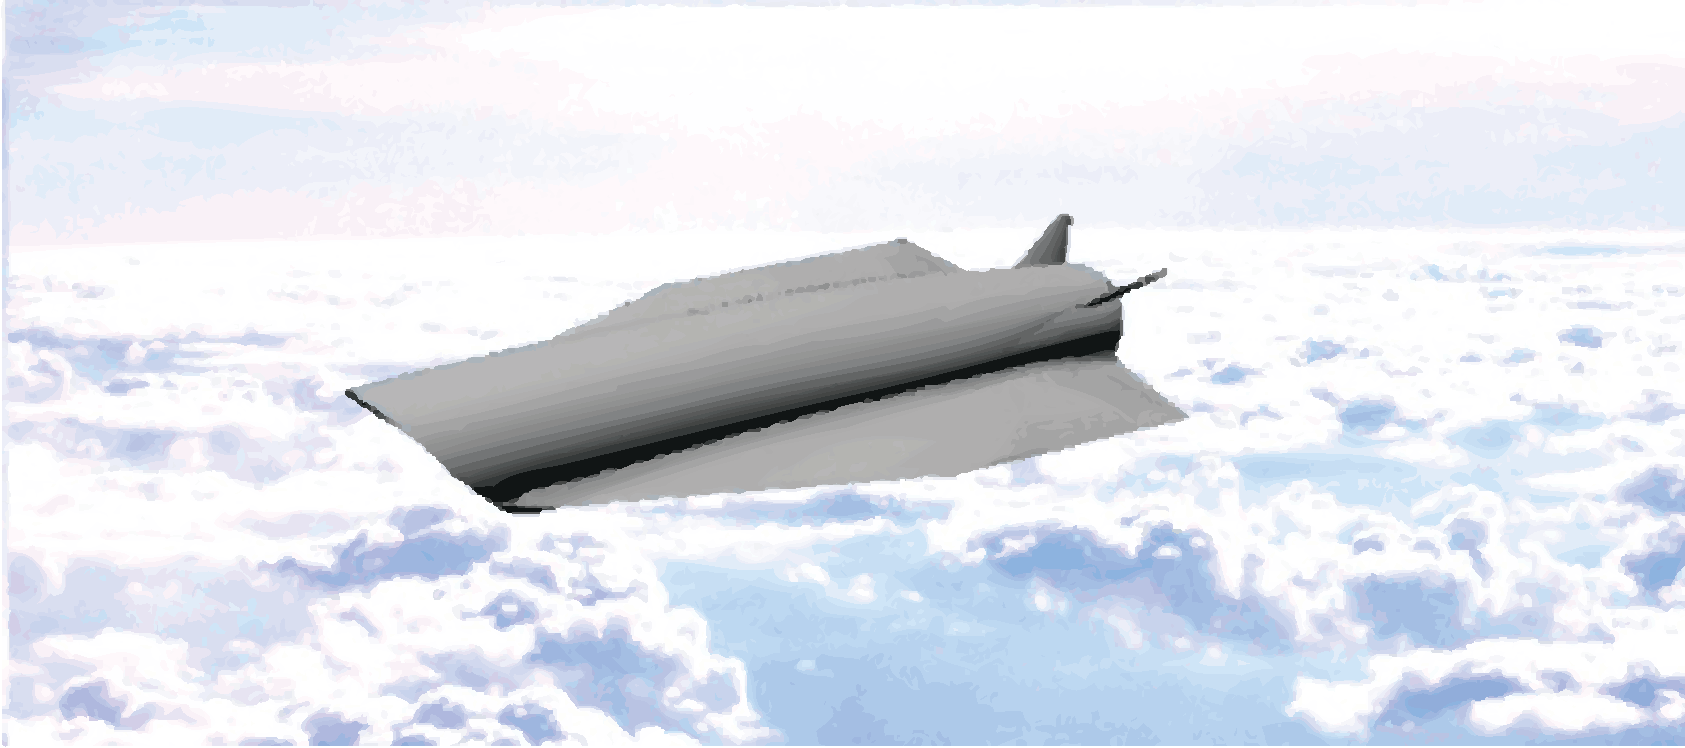
\includegraphics[width=6cm]{../fig/ghvclouds.pdf}};
  \path (naveq.145)+(-\blockdist,0) node (block1) [squareblock, minimum width=2.5cm] {Baseline};
  \path (naveq.-145)+(-\blockdist,0) node (block2) [squareblock, minimum width=2.5cm] {\shortstack{Adaptive \\ Augmentation}};
  %\node[squareblock, minimum height=1cm, minimum width=2cm, right of=block3, node distance=5.0cm] (block4) {\shortstack[c]{Error \\ Generator}};
  %\node[output, right of=block4,node distance=2.0cm] (output1) {};
  \path [draw, ->] (block1) -- (block3.west |- block1) ;
  \path [draw, ->] (block2) -- (block3.west |- block2);
  %\draw[->](block3) -- (block4);
  %\draw[->](block4) --  node[above,pos=0.8]{$e$}(output1);
\end{tikzpicture}

  \clearpage
\section*{\currfilename}

\begin{tikzpicture}
  \node (block3) [squareblock, label=below:{\shortstack[c]{\bf Nonlinear Equations\\ \bf of Motion}}, minimum width=6cm, inner sep=0mm] {\centering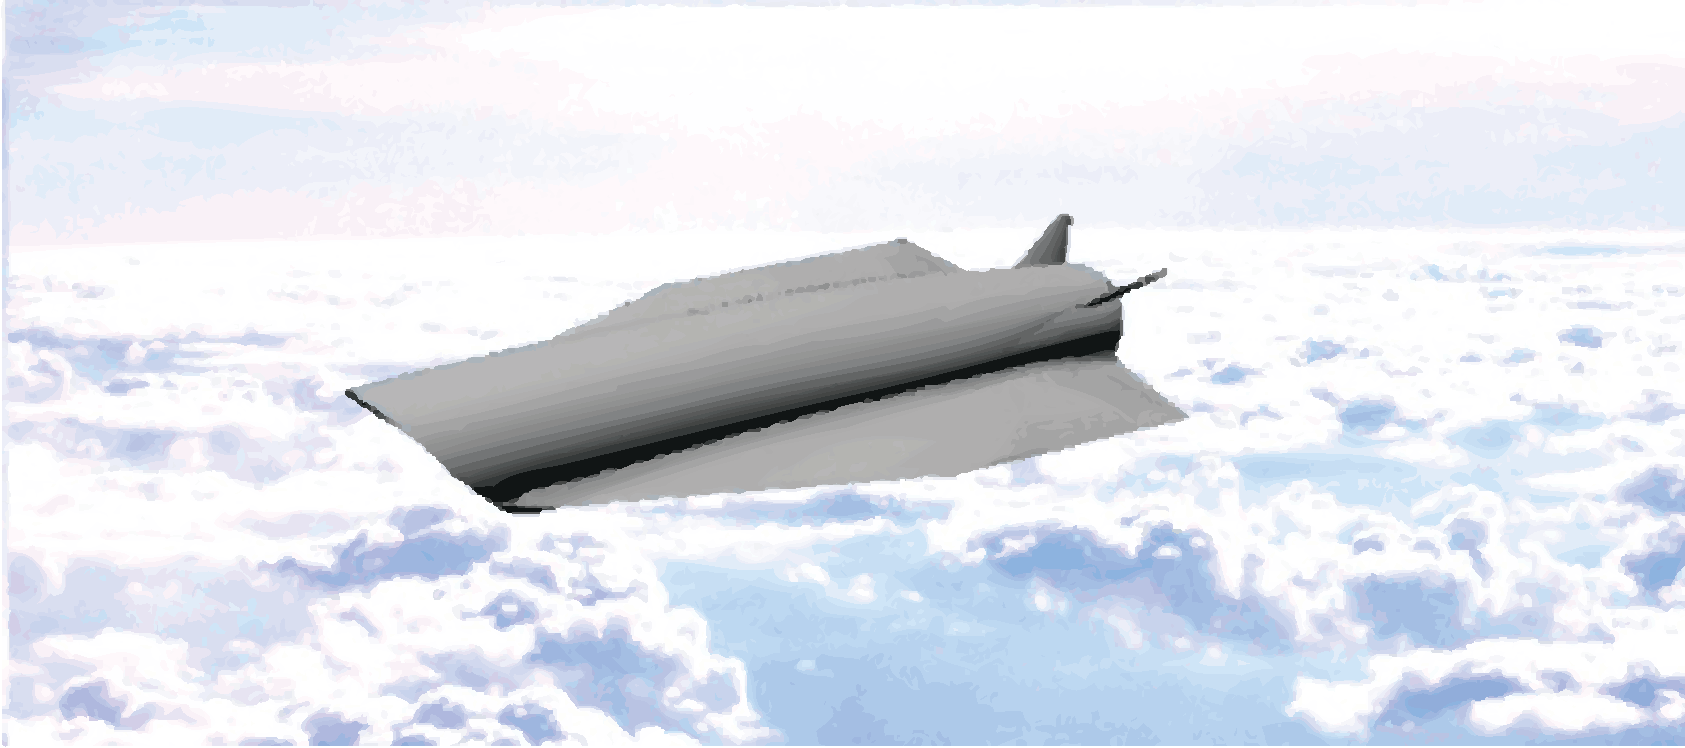
\includegraphics[width=6cm]{../fig/ghvclouds.pdf}};
  \path (naveq.145)+(-\blockdist,0) node (block1) [squareblock, minimum width=2.5cm] {Baseline};
  \path (naveq.-145)+(-\blockdist,0) node (block2) [squareblock, minimum width=2.5cm] {\shortstack{Adaptive \\ Augmentation}};
  \node[squareblock, below of=block2, node distance=1.5cm, minimum height=1cm, minimum width=2cm] (blockT){\fontsize{14pt}{14pt}\selectfont$\theta(t)$};
  \node[squareblock, minimum height=1cm, minimum width=2cm, right of=block3, node distance=5.0cm] (block4) {\shortstack[c]{Error \\ Generator}};
  \node[output, right of=block4,node distance=2.0cm] (output1) {};
  \node[input, below of=blockT, node distance=1.5cm] (input2) {};
  \path [draw, ->] (block1) -- (block3.west |- block1) ;
  \path [draw, ->] (block2) -- (block3.west |- block2);
  \draw[->](input2) -- node[left,pos=0.5]{$e$, $x$, $\Gamma$}(blockT);
  \draw[->](blockT) -- (block2);
  \draw[->](block3) -- (block4);
  \draw[->](block4) --  node[above,pos=0.8]{$e$}(output1);
\end{tikzpicture}

% \node (output1) [input, right of=sum1, node distance=1.5cm] {};
% \path [draw, ->] (block1) -- (block3.west |- block1) ;
% \path [draw, ->] (block2) -- (block3.west |- block2);
% \path [draw, ->] (block3) -- node[pos=0.7]{$-$} (sum1);
% \path [draw, ->] (input1) -- node[pos=0.2]{target} node[pos=0.7]{$+$} (sum1);
% \path [draw, ->] (sum1) -- node[pos=0.7]{error} (output1);
% \draw[->](block3) -- node[pos=0.7, anchor=north]{$-$} (sum1);


  \clearpage
\section*{\currfilename}

\pgfdeclarelayer{background}
\pgfdeclarelayer{foreground}
\pgfsetlayers{background,main,foreground}

% Define a few styles and constants
\tikzstyle{sensor}=[draw, fill=blue!20, text width=5em, text centered, minimum height=2.5em]
\tikzstyle{ann} = [above, text width=5em]
\tikzstyle{naveqs} = [sensor, text width=6em, fill=red!20, minimum height=12em, rounded corners]
\def\blockdist{5}
\def\edgedist{2.5}

\begin{tikzpicture}
  \node (block3) [squareblock, label=below:{\shortstack[c]{\bf Nonlinear Equations\\ \bf of Motion}}, minimum width=6cm, inner sep=0mm] {\centering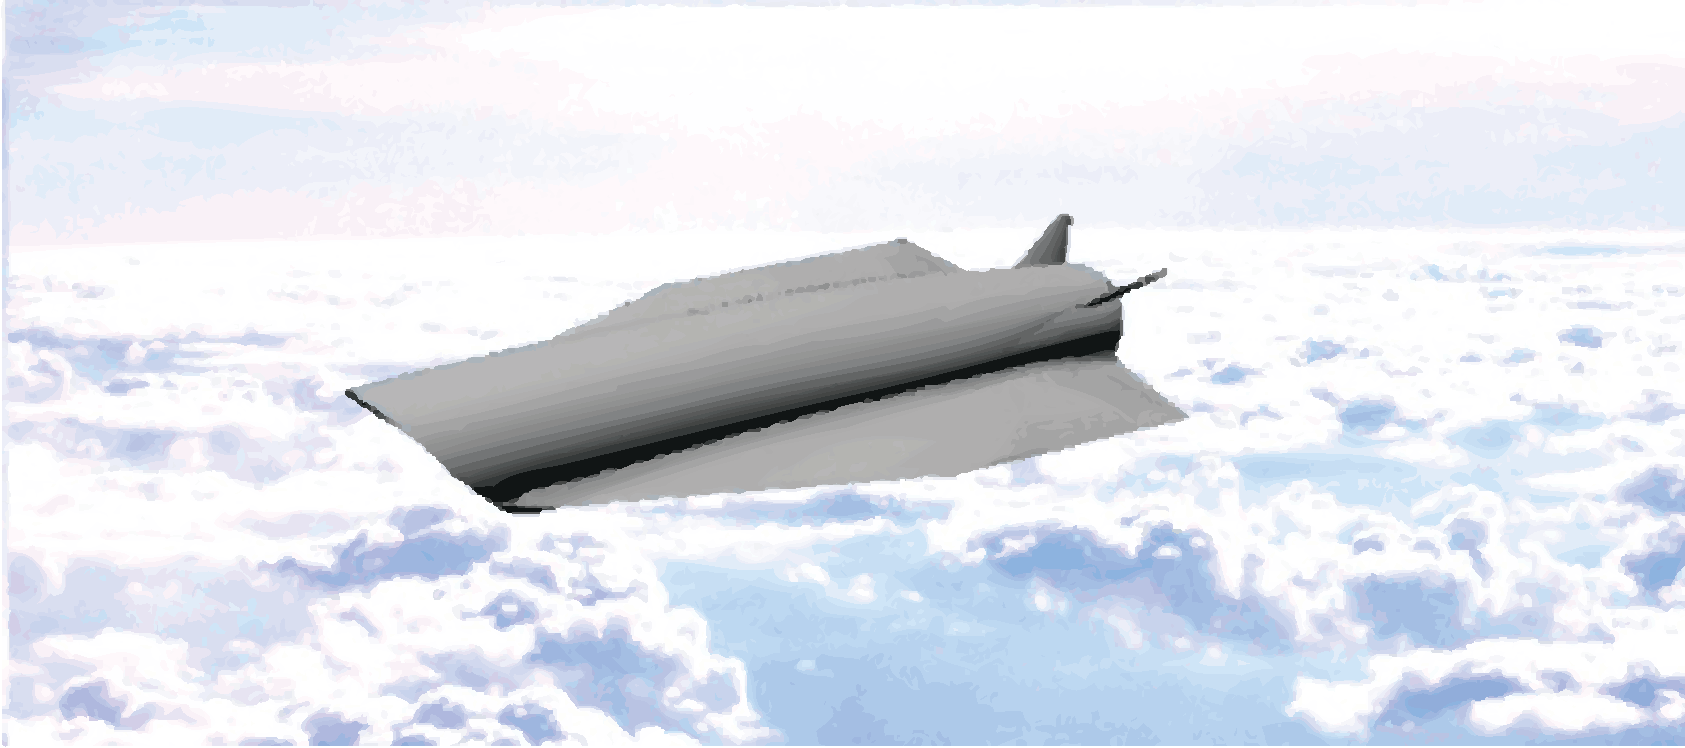
\includegraphics[width=6cm]{../fig/ghvclouds.pdf}};
  \node (summer) [whitesum, left of=block3, node distance=4cm] {};
  \path (naveq.145)+(-\blockdist,0) node (block1) [squareblock, minimum width=2.5cm] {Baseline};
  \path (naveq.-145)+(-\blockdist,0) node (block2) [squareblock, minimum width=2.5cm] {\shortstack{Adaptive \\ Augmentation}};
  \node[squareblock, minimum height=1cm, minimum width=2cm, right of=block3, node distance=5.0cm] (block4) {\shortstack[c]{Error \\ Generator}};
  \node[output, right of=block4,node distance=2.0cm] (output1) {};
  \draw[->](block1) -| node[right, pos=0.8]{$+$} (summer);
  \draw[->](block2) -| node[right, pos=0.8]{$+$} (summer);
  \draw[->](summer) -- node[above,pos=0.5]{$u$} (block3);
  \draw[->](block3) -- (block4);
  \draw[->](block4) --  node[above,pos=0.7]{$e$}(output1);
\end{tikzpicture}

  \clearpage
\section*{\currfilename}

\pgfdeclarelayer{background}
\pgfdeclarelayer{foreground}
\pgfsetlayers{background,main,foreground}

% Define a few styles and constants
\tikzstyle{sensor}=[draw, fill=blue!20, text width=5em, text centered, minimum height=2.5em]
\tikzstyle{ann} = [above, text width=5em]
\tikzstyle{naveqs} = [sensor, text width=6em, fill=red!20, minimum height=12em, rounded corners]
\def\blockdist{5}
\def\edgedist{2.5}

\begin{tikzpicture}
  \node (block3) [squareblock, label=below:{\shortstack[c]{\bf Nonlinear Equations\\ \bf of Motion}}, minimum width=6cm, inner sep=0mm] {\centering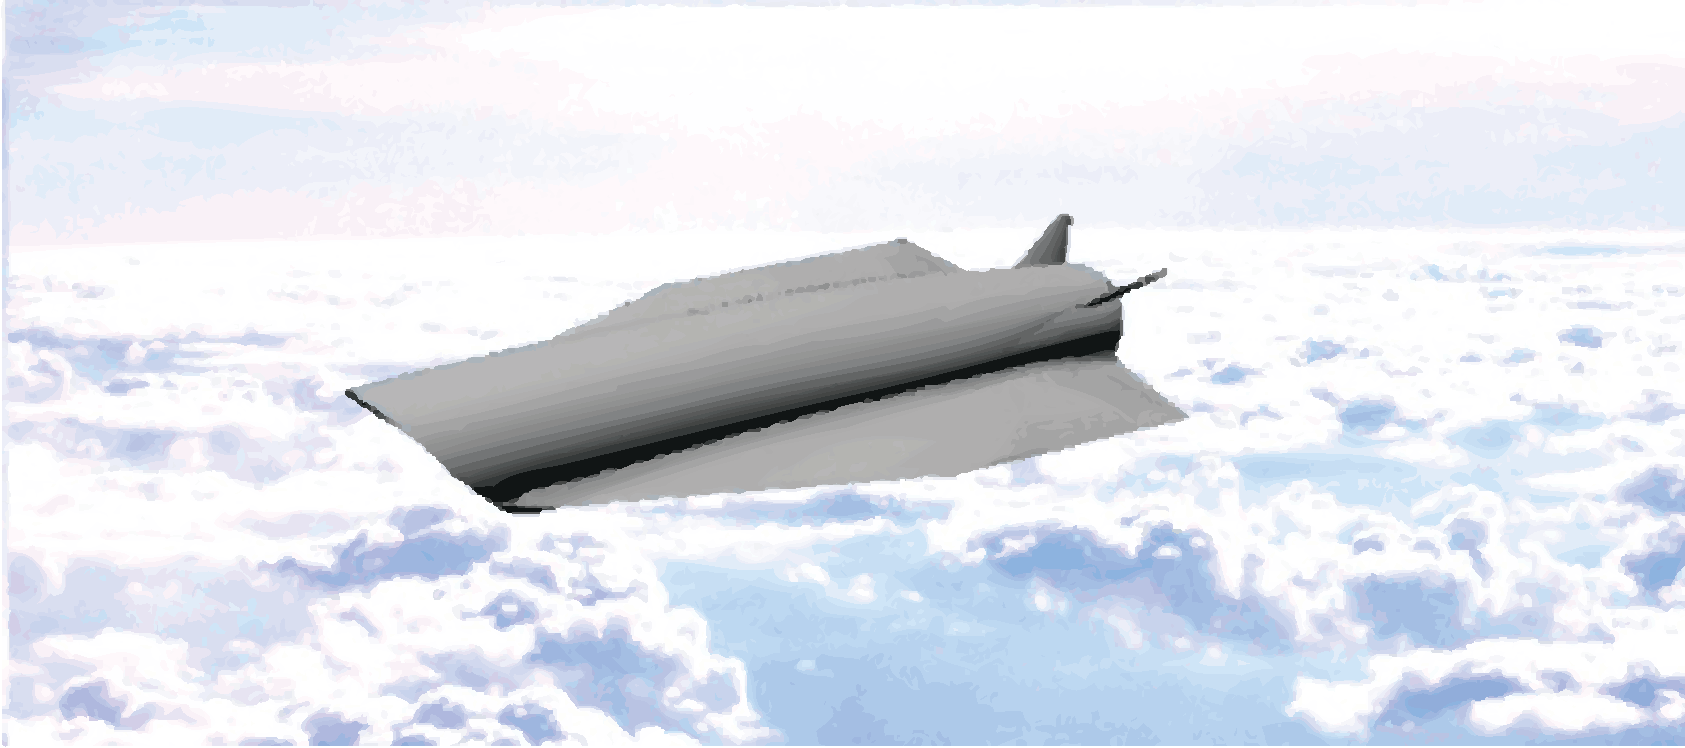
\includegraphics[width=6cm]{../fig/ghvclouds.pdf}};
  \node (summer) [whitesum, left of=block3, node distance=4cm] {};
  \path (naveq.145)+(-\blockdist,0) node (block1) [squareblock, minimum width=2.5cm] {Baseline};
  \path (naveq.-145)+(-\blockdist,0) node (block2) [squareblock, minimum width=2.5cm] {\shortstack{Adaptive \\ Augmentation}};
  \draw[->](block1) -| node[right, pos=0.8]{$+$} (summer);
  \draw[->](block2) -| node[right, pos=0.8]{$+$} (summer);
  \draw[->](summer) -- node[above,pos=0.5]{$u$} (block3);
  \draw[->](block3) -- (block4);
\end{tikzpicture}

  \clearpage
\section*{\currfilename}

\pgfdeclarelayer{background}
\pgfdeclarelayer{foreground}
\pgfsetlayers{background,main,foreground}
% Define a few styles and constants
\tikzstyle{sensor}=[draw, fill=blue!20, text width=5em, text centered, minimum height=2.5em]
\tikzstyle{ann} = [above, text width=5em]
\tikzstyle{naveqs} = [sensor, text width=6em, fill=red!20, minimum height=12em, rounded corners]
\def\blockdist{5}
\def\edgedist{2.5}

\begin{tikzpicture}
  \node (block3) [squareblock, label=below:{\shortstack[c]{\bf Nonlinear Equations\\ \bf of Motion}}, minimum width=6cm, inner sep=0mm] {\centering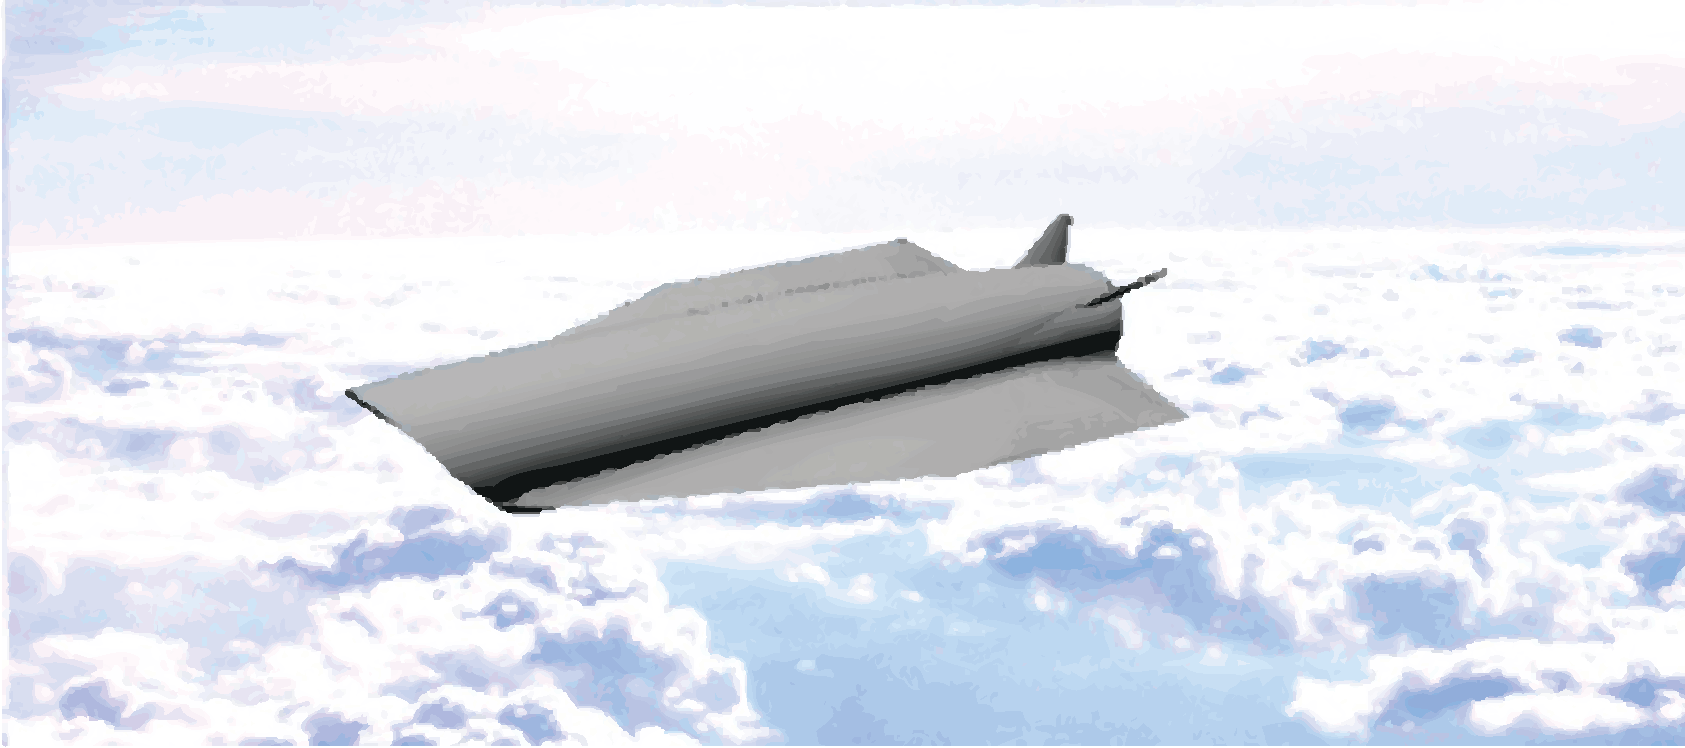
\includegraphics[width=6cm]{../fig/ghvclouds.pdf}};
  \node (summer) [whitesum, left of=block3, node distance=4cm] {};
  \path (naveq.145)+(-\blockdist,0) node (block1) [squareblock, minimum width=2.5cm] {Baseline};
  \draw[->](block1) -| node[right, pos=0.8]{$+$} (summer);
  \draw[->](summer) -- node[above,pos=0.5]{$u$} (block3);
  \draw[->](block3) -- (block4);
\end{tikzpicture}

  \clearpage
\section*{\currfilename}

\begin{figure}[H]
  \begin{center}
    \fontsize{10pt}{10pt}\selectfont
    \begin{tikzpicture}[auto, scale=1.0, every node/.style={transform shape}, node distance=1.0cm, >=latex']
      %\node[input, left of=input1, node distance=3cm] (input1) {};
      \node[squareblock, minimum height=1cm, minimum width=2cm] (block1){\shortstack[c]{Adaptive\\Controller}};
      \node[squareblock, below of=block1, node distance=1.5cm, minimum height=1cm, minimum width=2cm] (block2){\fontsize{14pt}{14pt}\selectfont$\theta(t)$};
      \node [right of=block1,draw=black, anchor=west,node distance=2.0cm, minimum width=2cm, inner sep= 0mm, label=below:{\shortstack[c]{\bf Nonlinear Equations\\ \bf of Motion}}] (block3) {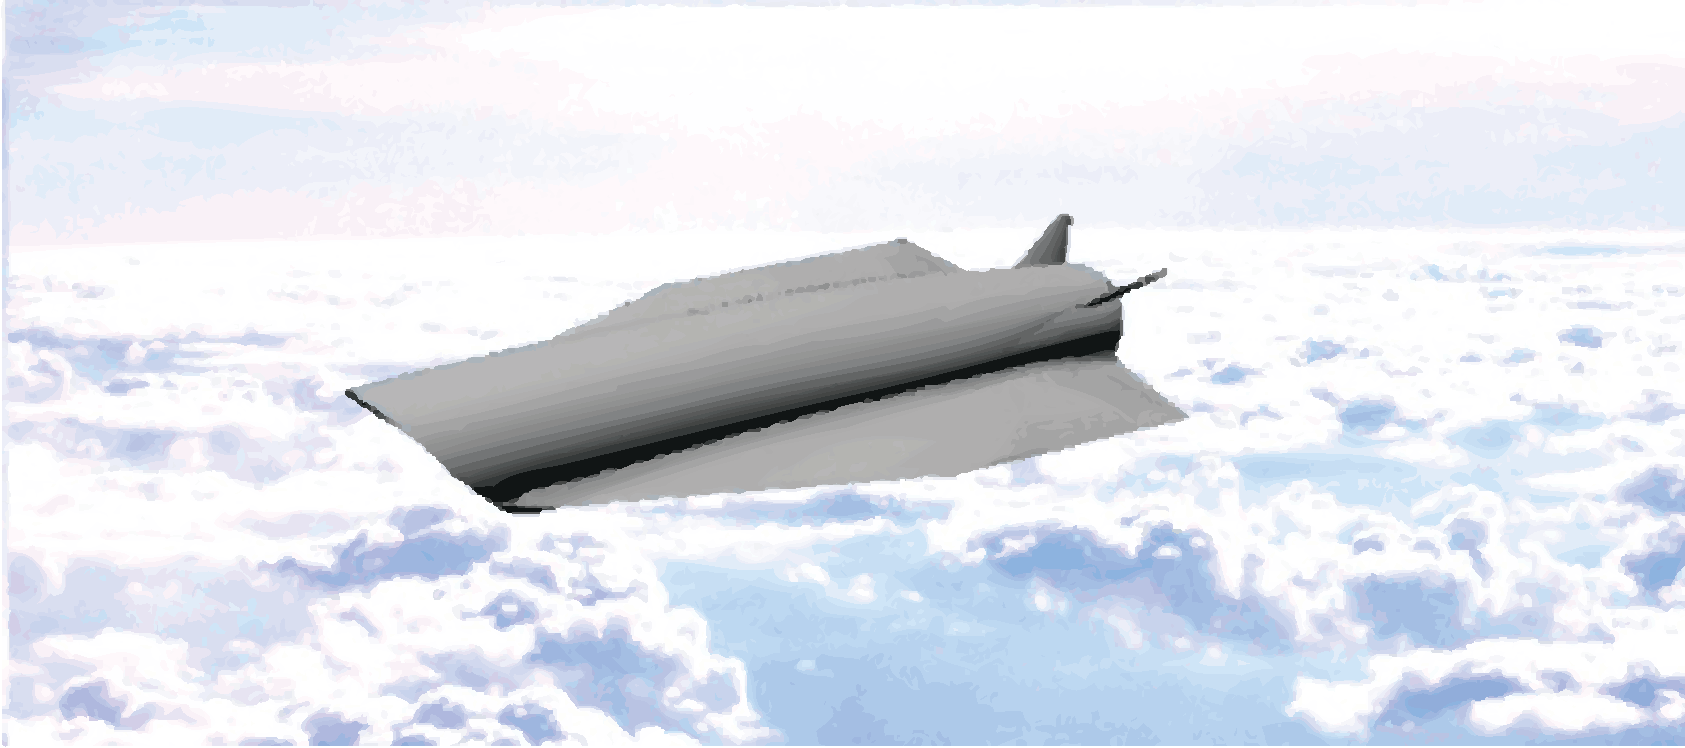
\includegraphics[width=4cm]{../fig/ghvclouds.pdf}};
      \node[squareblock, minimum height=1cm, minimum width=2cm, right of=block3, node distance=4.0cm] (block4) {\shortstack[c]{Error \\ Generator}};
      \node[output, right of=block4,node distance=2.0cm] (output1) {};
      \node[input, below of=block2, node distance=1.5cm] (input2) {};
      %\draw[->](input1) -- (block1);
      \draw[->](input2) -- node[pos=0.5]{$e$, $x$, $\Gamma$}(block2);
      \draw[->](block2) -- (block1);
      \draw[->](block1) -- (block3);
      \draw[->](block3) -- (block4);
      \draw[->](block4) --  node[pos=0.8]{$e$}(output1);
    \end{tikzpicture}
    \caption{Baseline plus adaptive control block diagram \label{fig.baseplusadaptiveblock}}
  \end{center}
\end{figure}

  \clearpage
\section*{\currfilename}

\begin{figure}[H]
  \fontsize{14pt}{14pt}\selectfont
  \begin{center}
    %\resizebox{1.7in}{0.5in}{
    \begin{tikzpicture}[auto, scale=1.0, every node/.style={transform shape}, node distance=3cm,>=latex']
      \matrix[ampersand replacement=\&, row sep=1.0cm, node distance=3.0cm] (regions) at (0,0){
      \node[block, minimum width=2cm, minimum height=1.5cm] (R1) {GHV}; \\
      };
      \matrix[ampersand replacement=\&, row sep=1.0cm, right of=R1, node distance=2.0cm] (R1out) {
      \node [whitesum] (R1outx) {};\\
      \node [coordinate] (R1outP) {};\\
      };
      \node[output, right of=R1outx,node distance=1.0cm](output1){};
      \node[output, below of=output1,node distance=1.0cm](output2){};
      \node [coordinate, left of=R1, node distance=2.0cm] (input1) {};
      \node[input, above of=R1outx,node distance=1.0cm](input2){};
      %draw
      \draw [->] (input1) -- node [near start]{$u$} (R1);
      \draw [->] (input2) -- node [near start]{unknown bias} (R1outx);
      \draw [->] (R1.east) + (0cm,0.5cm) -- (R1outx);
      \draw [->] (R1outx) -- node [pos=0.9]{} (output1);
      \draw [->] (R1.east) + (0cm,-0.5cm) -- node [pos=0.95]{} (output2);
      %cross out
      \coordinate (arrow1) at ([xshift=-0.4cm,yshift=-0.3cm] output1);
      \coordinate (arrow2) at ([xshift=0.2cm,yshift=0.3cm] output1);
      \coordinate (arrow3) at ([xshift=-0.4cm,yshift=0.3cm] output1);
      \coordinate (arrow4) at ([xshift=0.2cm,yshift=-0.3cm] output1);
      \draw[-,red,line width=2](arrow1) -- (arrow2);
      \draw[-,red,line width=2](arrow3) -- (arrow4);
      \node [right of=output1, node distance = 2.0cm] {$\beta$ is corrupted};
      \node [right of=output2, node distance = 0.8cm] {$p$, $r$, $\phi$};
    \end{tikzpicture}
    %}
  \end{center}
\end{figure}

  \clearpage
\section*{\currfilename}

\begin{figure}[H]
  \fontsize{14pt}{14pt}\selectfont
  \begin{center}
    %\resizebox{1.7in}{0.5in}{
    \begin{tikzpicture}[auto, scale=1.0, every node/.style={transform shape}, node distance=3cm,>=latex']
      \matrix[ampersand replacement=\&, row sep=1.0cm, node distance=3.0cm] (regions) at (0,0){
      \node[block, minimum width=2cm, minimum height=1.5cm] (R1) {GHV}; \\
      };
      \matrix[ampersand replacement=\&, row sep=1.0cm, right of=R1, node distance=2.0cm] (R1out) {
      \node [coordinate] (R1outx) {};\\
      \node [coordinate] (R1outP) {};\\
      };
      \node[output, right of=R1outx,node distance=0.5cm](output1){};
      \node[output, below of=output1,node distance=1.0cm](output2){};
      %\node [coordinate, left of=R1, node distance=2.0cm] (input1) {};
      %\node[input, above of=R1outx,node distance=1.0cm](input2){};
      %draw
      \draw [->] (input1) -- node [near start]{$u$} (R1);
      %\draw [->] (input2) -- node [near start]{unknown bias} (R1outx);
      \draw [->] (R1.east) + (0cm,0.5cm) -- (output1);
      %\draw [->] (R1outx) -- node [pos=0.9]{} (output1);
      \draw [->] (R1.east) + (0cm,-0.5cm) -- node [pos=0.95]{} (output2);
      %cross out
      \coordinate (arrow1) at ([xshift=-0.4cm,yshift=-0.3cm] output1);
      \coordinate (arrow2) at ([xshift=0.2cm,yshift=0.3cm] output1);
      \coordinate (arrow3) at ([xshift=-0.4cm,yshift=0.3cm] output1);
      \coordinate (arrow4) at ([xshift=0.2cm,yshift=-0.3cm] output1);
      \draw[-,red,line width=2](arrow1) -- (arrow2);
      \draw[-,red,line width=2](arrow3) -- (arrow4);
      \node [right of=output1, node distance = 2.0cm] {$\beta$ unavailable};
      \node [right of=output2, node distance = 1.8cm] {$y=[\;p\;r\;\phi\;]^{\top}$};
    \end{tikzpicture}
    %}
  \end{center}
\end{figure}

  \clearpage
\section*{\currfilename}

\begin{figure}[H]
  \fontsize{10pt}{10pt}\selectfont
  \begin{center}
    \begin{tikzpicture}[auto, scale=1.0, every node/.style={transform shape}, node distance=3cm,>=latex']
      \matrix[ampersand replacement=\&, row sep=1.0cm, node distance=3.0cm] (regions) at (0,0){
      \node [draw=black, label=below:{\shortstack[c]{GHV Equations\\ of Motion}}, label=above:{$A,B\Lambda,C$}, minimum width=2cm, inner sep=0mm] (R1){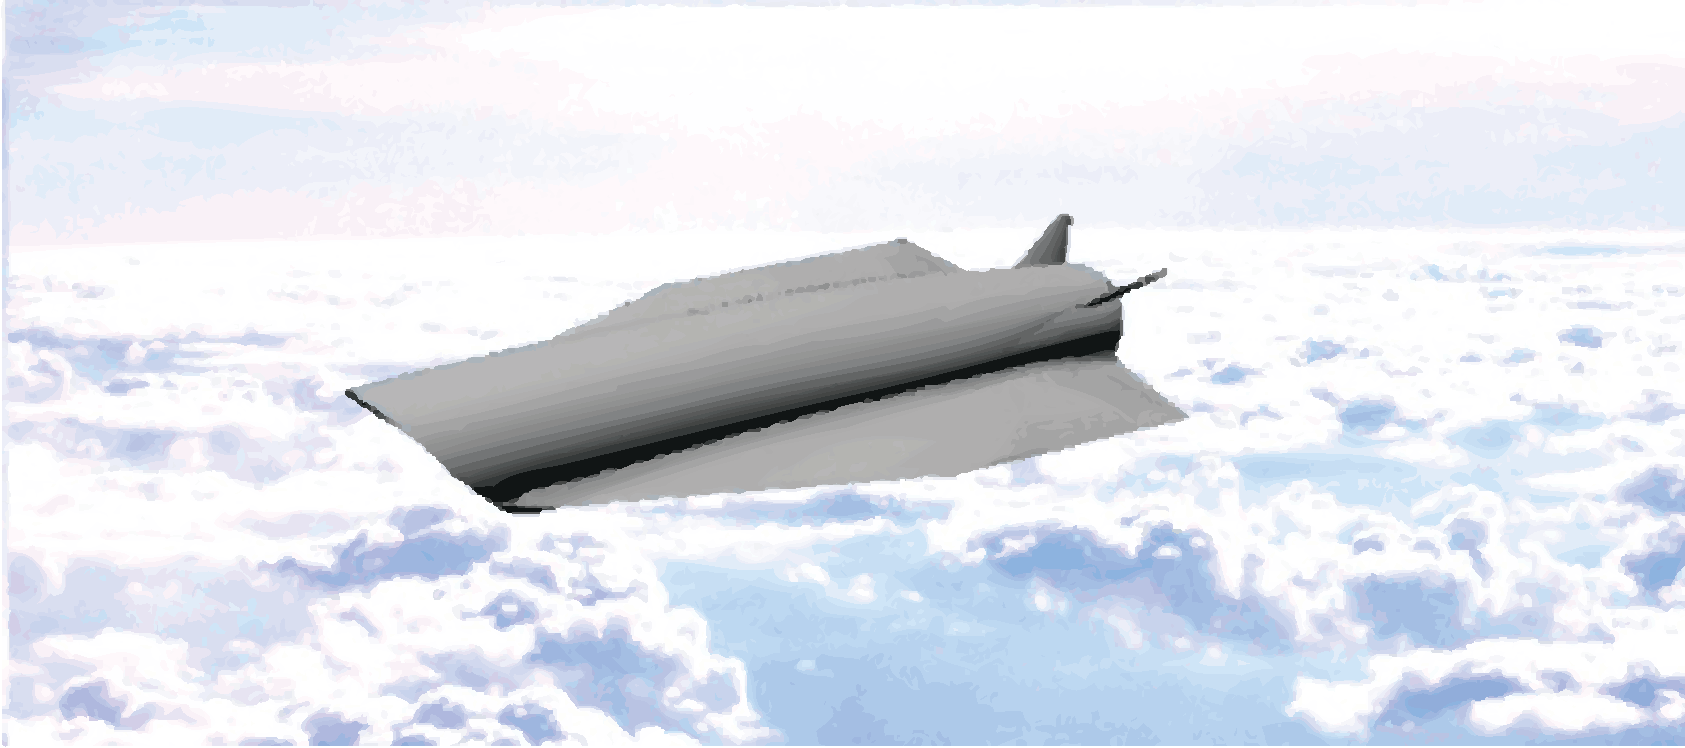
\includegraphics[width=4cm]{../fig/ghvclouds.pdf}}; \\
      };
      \matrix[ampersand replacement=\&, row sep=1.0cm, right of=R1, node distance=3.0cm] (R1out) {
        \node [whitesum] (R1outx) {}; \\
        \node [coordinate] (R1outP) {}; \\
      };
      \node[output, right of=R1outx,node distance=1.5cm](output1){};
      \node[output, below of=output1,node distance=1.0cm](output2){};
      \matrix[ampersand replacement=\&, row sep=0.6cm, left of=R1, node distance=4.0cm] (regions) {
        \node [block] (block2){\shortstack[c]{Adaptive\\ Controller}}; \\
      };
      \matrix[ampersand replacement=\&, row sep=0.6cm, left of=block2, node distance=3.0cm] (b2out) {
        \node [coordinate] (b2out1) {}; \\
        \node [coordinate] (b2out2) {}; \\
      };
      \node [coordinate, left of=b2out1, node distance=3.0cm] (input1) {};
      \node [coordinate, left of=b2out2, node distance=3.0cm] (input3) {};
      \node[input, above of=R1outx,node distance=1.0cm](input2){};
      \node[input, below of=block2,node distance=1.5cm](input4){};

      % Draw
      \draw [<-] (block2.west) + (0cm,0.3cm) -- node [near end]{$z_{\text{cmd}}$} (b2out1);
      \draw [<-] (block2.west) + (0cm,-0.3cm) -- node [near end]{$y$} (b2out2);
      \draw [->] (R1outx) -- node [pos=0.9]{} (output1);
      \draw [->] (block2) -- node [near start]{$u$} (R1);
      \draw [->] (input2) -- node [near start]{bias} (R1outx);
      \draw [->] (R1.east) + (0cm,0.5cm) -- (R1outx);
      \draw [->] (R1outx) -- node [pos=0.9]{} (output1);
      \draw [->] (R1.east) + (0cm,-0.5cm) -- node [pos=0.95]{$y$} (output2);
      \draw [->] (input4) -- node [near start]{$S_{1}$, $L$} (block2);

      % Cross out
      \coordinate (arrow1) at ([xshift=-0.4cm,yshift=-0.3cm] output1);
      \coordinate (arrow2) at ([xshift=0.2cm,yshift=0.3cm] output1);
      \coordinate (arrow3) at ([xshift=-0.4cm,yshift=0.3cm] output1);
      \coordinate (arrow4) at ([xshift=0.2cm,yshift=-0.3cm] output1);
      \draw[-,red,line width=2](arrow1) -- (arrow2);
      \draw[-,red,line width=2](arrow3) -- (arrow4);
    \end{tikzpicture}
  \end{center}
\end{figure}

  \clearpage
\section*{\currfilename}

\begin{figure}[H]
  \fontsize{10pt}{10pt}\selectfont
  \begin{center}
    \begin{tikzpicture}[auto, scale=1.0, every node/.style={transform shape}, node distance=3cm,>=latex']
      \matrix[ampersand replacement=\&, row sep=1.0cm, node distance=3.0cm] (regions) at (0,0){
        \node [draw=black, label=below:{\shortstack[c]{GHV Equations\\ of Motion}}, label=above:{}, minimum width=2cm, inner sep=0mm] (R1){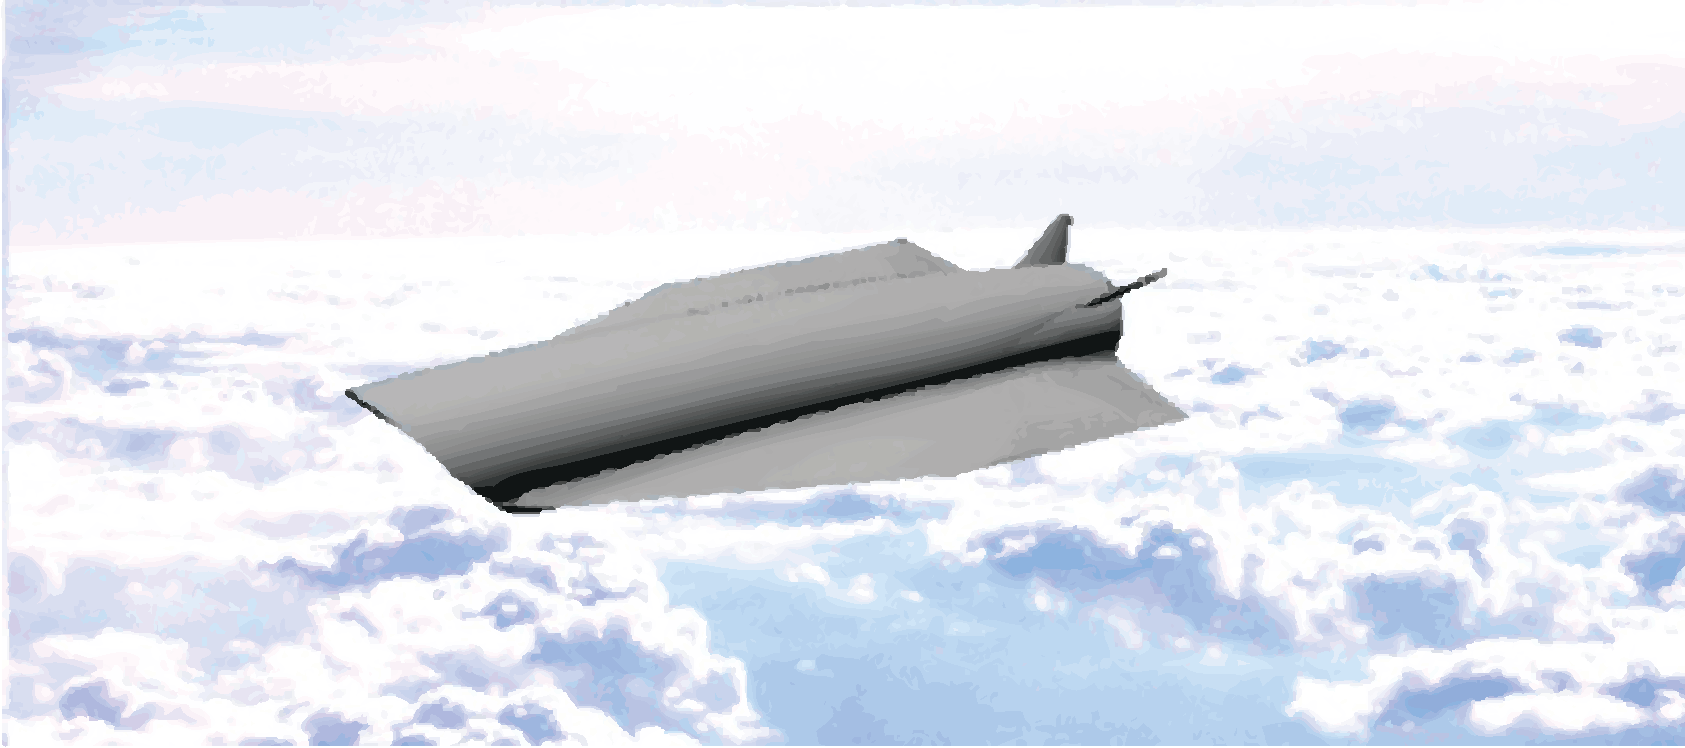
\includegraphics[width=4cm]{../fig/ghvclouds.pdf}}; \\
      };
      \matrix[ampersand replacement=\&, row sep=1.0cm, right of=R1, node distance=3.0cm] (R1out) {
        \node [whitesum] (R1outx) {}; \\
        \node [coordinate] (R1outP) {}; \\
      };
      \node[output, right of=R1outx,node distance=1.5cm](output1){};
      \node[output, below of=output1,node distance=1.0cm](output2){};
      \matrix[ampersand replacement=\&, row sep=0.6cm, left of=R1, node distance=4.0cm] (regions) {
        \node [block] (block2){\shortstack[c]{Adaptive\\ Controller}}; \\
      };
      \matrix[ampersand replacement=\&, row sep=0.6cm, left of=block2, node distance=3.0cm] (b2out) {
        \node [coordinate] (b2out1) {}; \\
        \node [coordinate] (b2out2) {}; \\
      };
      \node [coordinate, left of=b2out1, node distance=3.0cm] (input1) {};
      \node [coordinate, left of=b2out2, node distance=3.0cm] (input3) {};
      \node[input, above of=R1outx,node distance=1.0cm](input2){};
      \node[input, below of=block2,node distance=1.5cm](input4){};

      % Draw
      \draw [<-] (block2.west) + (0cm,0.3cm) -- node [near end]{$z_{p,\text{cmd}}$} (b2out1);
      \draw [<-] (block2.west) + (0cm,-0.3cm) -- node [near end]{$y$} (b2out2);
      \draw [->] (R1outx) -- node [pos=0.9]{} (output1);
      \draw [->] (block2) -- node [near start]{$u$} (R1);
      \draw [->] (input2) -- node [near start]{bias} (R1outx);
      \draw [->] (R1.east) + (0cm,0.5cm) -- (R1outx);
      \draw [->] (R1outx) -- node [pos=0.9]{} (output1);
      \draw [->] (R1.east) + (0cm,-0.5cm) -- node [pos=0.95]{$y$} (output2);
      \draw [->] (input4) -- node [near start]{$S_{1}$, $L$} (block2);

      % Cross out
      \coordinate (arrow1) at ([xshift=-0.4cm,yshift=-0.3cm] output1);
      \coordinate (arrow2) at ([xshift=0.2cm,yshift=0.3cm] output1);
      \coordinate (arrow3) at ([xshift=-0.4cm,yshift=0.3cm] output1);
      \coordinate (arrow4) at ([xshift=0.2cm,yshift=-0.3cm] output1);

      \draw[-,red,line width=2](arrow1) -- (arrow2);
      \draw[-,red,line width=2](arrow3) -- (arrow4);
    \end{tikzpicture}
  \end{center}
\end{figure}

  \clearpage
\section*{\currfilename}

\begin{figure}[H]
  \fontsize{10pt}{10pt}\selectfont
  \begin{center}
    \begin{tikzpicture}[auto, scale=1.0, every node/.style={transform shape}, node distance=3cm,>=latex']
      \matrix[ampersand replacement=\&, row sep=1.0cm, node distance=3.0cm] (regions) at (0,0){
        \node [draw=black, label=below:{\shortstack[c]{GHV Equations\\ of Motion}}, label=above:{$A,B\Lambda,C$}, minimum width=2cm, inner sep=0mm] (R1){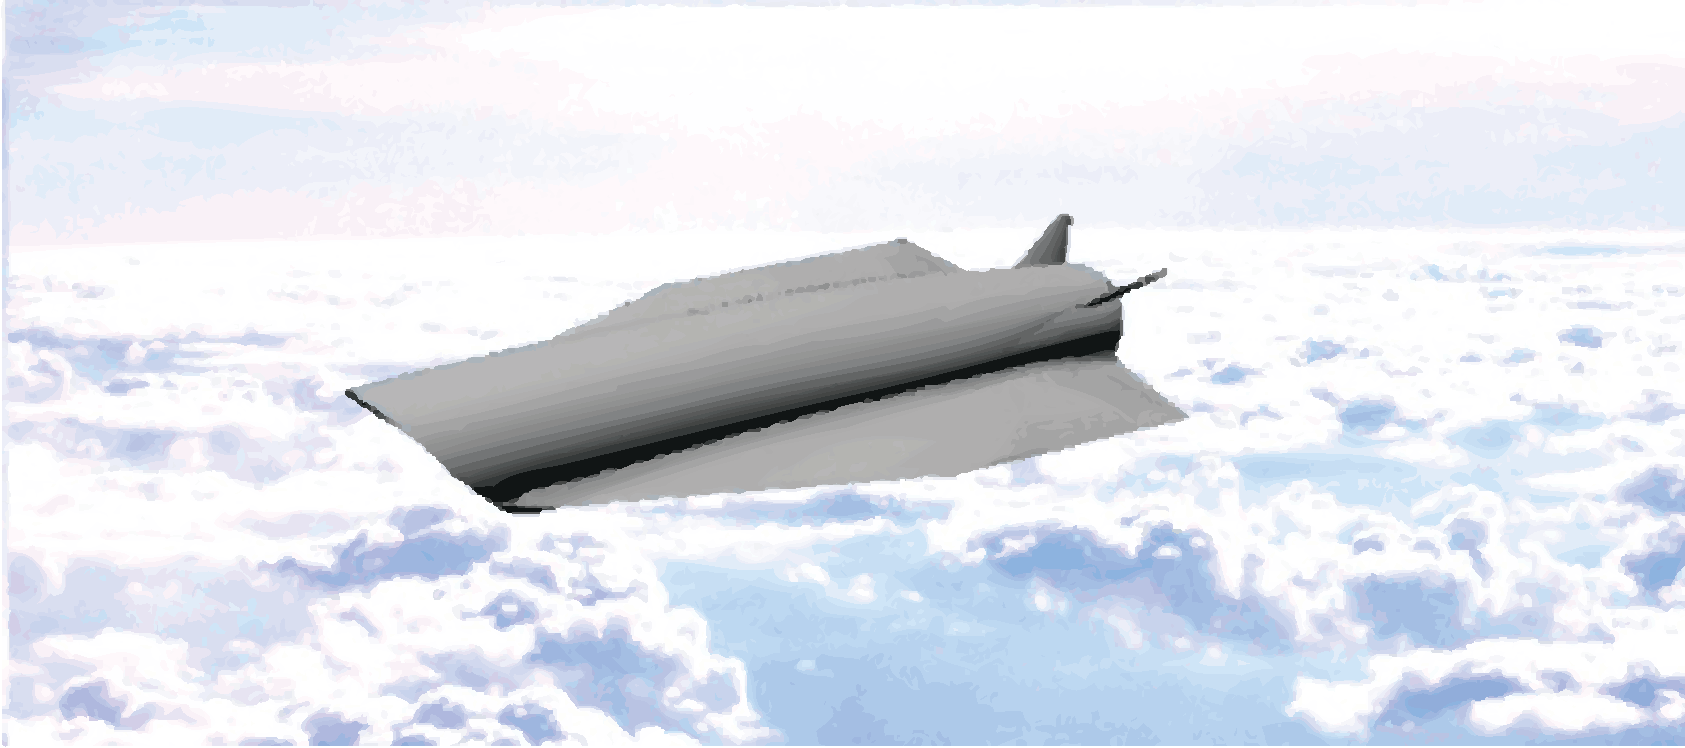
\includegraphics[width=4cm]{../fig/ghvclouds.pdf}}; \\
      };
      \matrix[ampersand replacement=\&, row sep=1.0cm, right of=R1, node distance=3.0cm] (R1out) {
        \node [whitesum] (R1outx) {}; \\
        \node [coordinate] (R1outP) {}; \\
      };
      \node[output, right of=R1outx,node distance=1.5cm](output1){};
      \node[output, below of=output1,node distance=1.0cm](output2){};
      \matrix[ampersand replacement=\&, row sep=0.6cm, left of=R1, node distance=4.0cm] (regions) {
        \node [block] (block2){\shortstack[c]{Adaptive\\ Controller}}; \\
      };
      \matrix[ampersand replacement=\&, row sep=0.6cm, left of=block2, node distance=3.0cm] (b2out) {
        \node [coordinate] (b2out1) {}; \\
        \node [coordinate] (b2out2) {}; \\
      };
      \node [coordinate, left of=b2out1, node distance=3.0cm] (input1) {};
      \node [coordinate, left of=b2out2, node distance=3.0cm] (input3) {};
      \node[input, above of=R1outx,node distance=1.0cm](input2){};
      \node[input, below of=block2,node distance=1.5cm](input4){};

      % Draw
      \draw [<-] (block2.west) + (0cm,0.3cm) -- node [near end]{$z_{\text{cmd}}$} (b2out1);
      \draw [<-] (block2.west) + (0cm,-0.3cm) -- node [near end]{$y$} (b2out2);
      \draw [->] (R1outx) -- node [pos=0.9]{} (output1);
      \draw [->] (block2) -- node [near start]{$u$} (R1);
      \draw [->] (input2) -- node [near start]{bias} (R1outx);
      \draw [->] (R1.east) + (0cm,0.5cm) -- (R1outx);
      \draw [->] (R1outx) -- node [pos=0.9]{} (output1);
      \draw [->] (R1.east) + (0cm,-0.5cm) -- node [pos=0.95]{$y$} (output2);
      %\draw [->] (input4) -- node [near start]{$S_{1}$, $L$} (block2);

      % Cross out
      \coordinate (arrow1) at ([xshift=-0.4cm,yshift=-0.3cm] output1);
      \coordinate (arrow2) at ([xshift=0.2cm,yshift=0.3cm] output1);
      \coordinate (arrow3) at ([xshift=-0.4cm,yshift=0.3cm] output1);
      \coordinate (arrow4) at ([xshift=0.2cm,yshift=-0.3cm] output1);
      \draw[-,red,line width=2](arrow1) -- (arrow2);
      \draw[-,red,line width=2](arrow3) -- (arrow4);
    \end{tikzpicture}
  \end{center}
\end{figure}


  \clearpage
\section*{\currfilename}

\begin{figure}[H]
  \fontsize{10pt}{10pt}\selectfont
  \begin{center}
    \begin{tikzpicture}[auto, scale=1.0, every node/.style={transform shape}, node distance=3cm,>=latex']
      \matrix[ampersand replacement=\&, row sep=1.0cm, node distance=3.0cm] (regions) at (0,0){
      \node [draw=black, label=below:{\shortstack[c]{GHV Equations\\ of Motion}}, label=above:{}, minimum width=2cm, inner sep=0mm] (R1){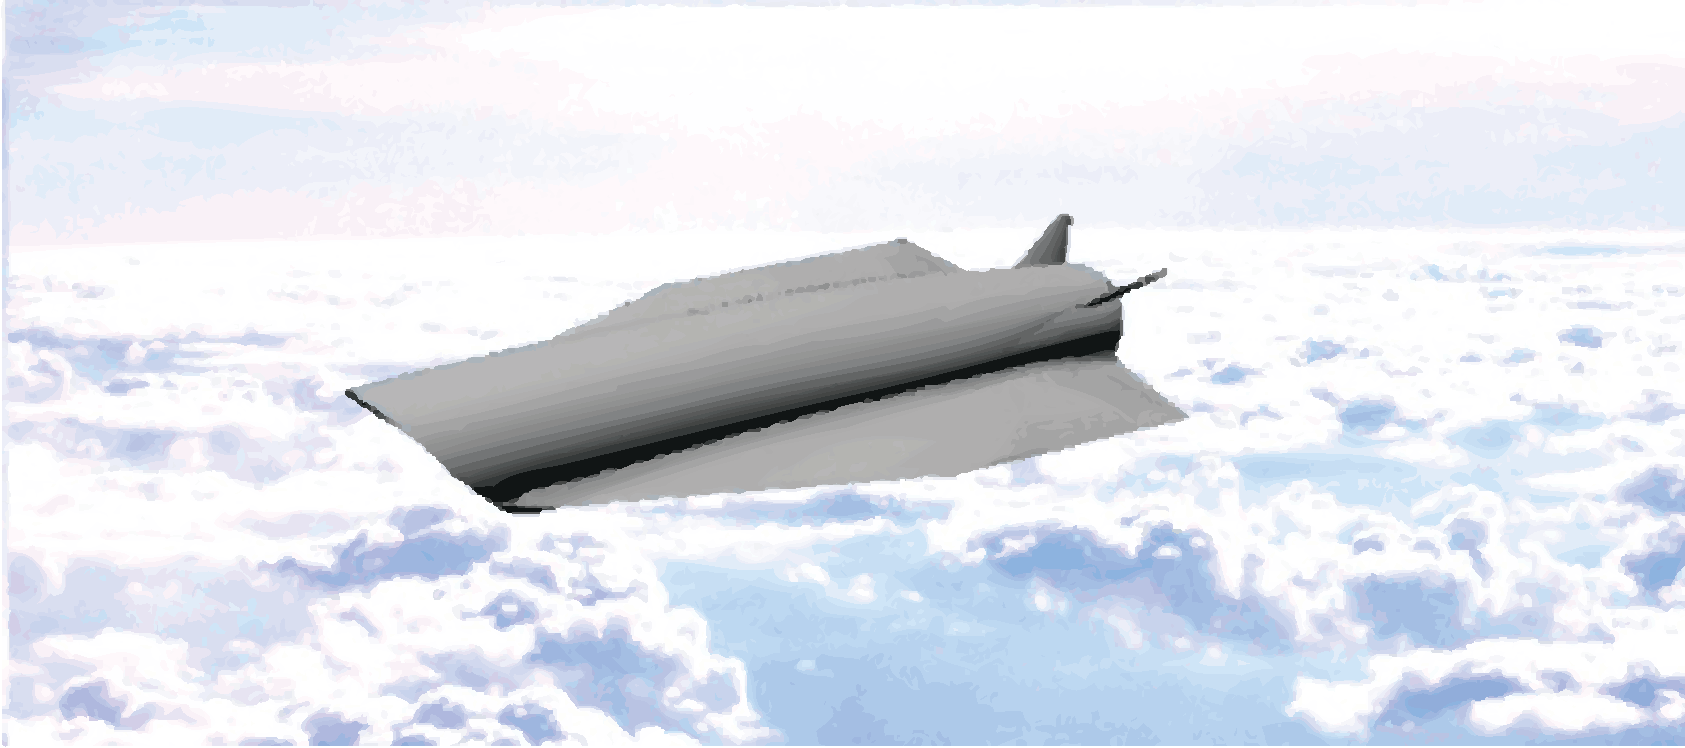
\includegraphics[width=4cm]{../fig/ghvclouds.pdf}}; \\
      };
      \matrix[ampersand replacement=\&, row sep=1.0cm, right of=R1, node distance=3.0cm] (R1out) {
        \node [coordinate] (R1outx) {}; \\
        \node [coordinate] (R1outP) {}; \\
      };
      \node[output, right of=R1outx,node distance=0.5cm](output1){};
      \node[output, below of=output1,node distance=1.0cm](output2){};
      \matrix[ampersand replacement=\&, row sep=0.6cm, left of=R1, node distance=4.0cm] (regions) {
        \node [block] (block2){\shortstack[c]{Adaptive\\ Controller}}; \\
      };
      \matrix[ampersand replacement=\&, row sep=0.6cm, left of=block2, node distance=3.0cm] (b2out) {
        \node [coordinate] (b2out1) {}; \\
        \node [coordinate] (b2out2) {}; \\
      };
      \node [coordinate, left of=b2out1, node distance=3.0cm] (input1) {};
      \node [coordinate, left of=b2out2, node distance=3.0cm] (input3) {};
      \node[input, above of=R1outx,node distance=1.0cm](input2){};
      \node[input, below of=block2,node distance=1.5cm](input4){};

      % Draw
      \draw [<-] (block2.west) + (0cm,0.3cm) -- node [near end]{$\phi_{\text{cmd}}$} (b2out1);
      \draw [<-] (block2.west) + (0cm,-0.3cm) -- node [near end]{$y$} (b2out2);
      \draw [->] (R1outx) -- node [pos=0.9]{} (output1);
      \draw [->] (block2) -- node [near start]{$u$} (R1);
      %\draw [->] (input2) -- node [near start]{bias} (R1outx);
      \draw [-] (R1.east) + (0cm,0.5cm) -- (R1outx);
      \draw [->] (R1outx) -- node [pos=0.9]{} (output1);
      \draw [->] (R1.east) + (0cm,-0.5cm) -- node [pos=0.95]{$y$} (output2);
      %\draw [->] (input4) -- node [near start]{$S_{1}$, $L$} (block2);

      % Cross out
      \coordinate (arrow1) at ([xshift=-0.4cm,yshift=-0.3cm] output1);
      \coordinate (arrow2) at ([xshift=0.2cm,yshift=0.3cm] output1);
      \coordinate (arrow3) at ([xshift=-0.4cm,yshift=0.3cm] output1);
      \coordinate (arrow4) at ([xshift=0.2cm,yshift=-0.3cm] output1);
      \draw[-,red,line width=2](arrow1) -- (arrow2);
      \draw[-,red,line width=2](arrow3) -- (arrow4);
    \end{tikzpicture}
  \end{center}
\end{figure}

  \clearpage
\section*{\currfilename}

\pgfdeclarelayer{background}
\pgfdeclarelayer{foreground}
\pgfsetlayers{background,main,foreground}

% Define a few styles and constants
\tikzstyle{sensor}=[draw, fill=blue!20, text width=5em, text centered, minimum height=2.5em]
\tikzstyle{ann} = [above, text width=5em]
\tikzstyle{naveqs} = [sensor, text width=6em, fill=red!20, minimum height=12em, rounded corners]
\def\blockdist{5}
\def\edgedist{2.5}

\begin{tikzpicture}
  \node (block3) [squareblock, label=below:{\shortstack[c]{\bf Nonlinear Equations\\ \bf of Motion}}, minimum width=6cm, inner sep=0mm] {\centering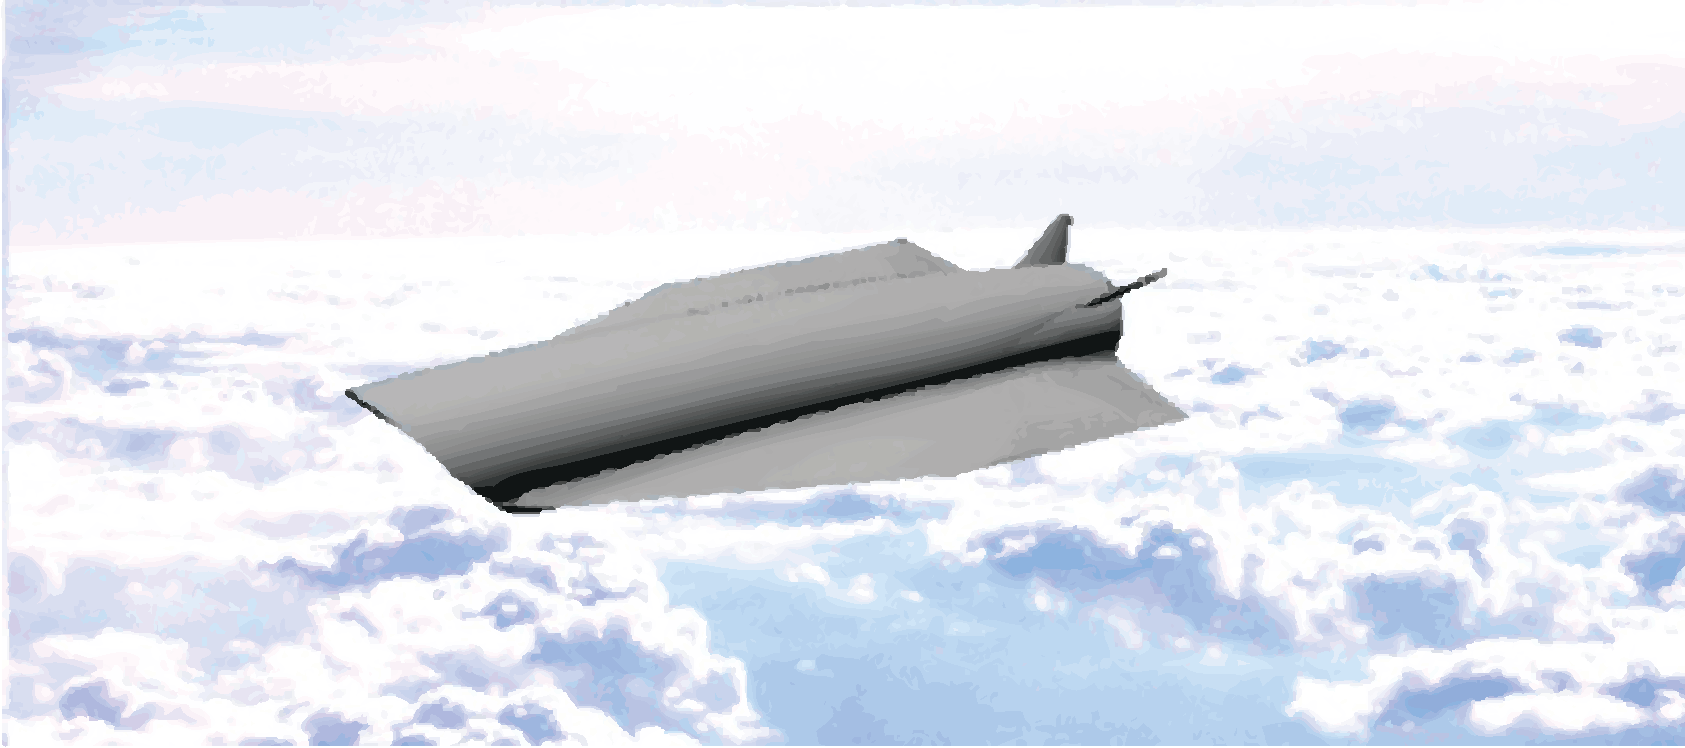
\includegraphics[width=6cm]{../fig/ghvclouds.pdf}};
  \node (summer) [whitesum, left of=block3, node distance=4cm] {};
  \path (naveq.145)+(-\blockdist,0) node (block1) [squareblock, minimum width=2.5cm] {Baseline};
  \path (naveq.-145)+(-\blockdist,0) node (block2) [squareblock, minimum width=2.5cm] {\shortstack{Adaptive \\ Augmentation}};
  \node[squareblock, minimum height=1cm, minimum width=2cm, right of=block3, node distance=5.0cm] (block4) {\shortstack[c]{Error \\ Generator}};
  \node[output, right of=block4,node distance=2.0cm] (output1) {};
  \draw[->](block1) -| node[right, pos=0.8]{$+$} (summer);
  \draw[->](block2) -| node[right, pos=0.8]{$+$} (summer);
  \draw[->](summer) -- node[above,pos=0.5]{$u$} (block3);
  \draw[->](block3) -- (block4);
  \draw[->](block4) --  node[above,pos=0.7]{$e$}(output1);
\end{tikzpicture}

  \clearpage
\section*{\currfilename}

\begin{figure}[H]
  \fontsize{10pt}{10pt}\selectfont
  \begin{center}
    \begin{tikzpicture}[auto, scale=1.0, every node/.style={transform shape}, node distance=1.0cm, >=latex']
      \node[squareblock, minimum height=1cm, minimum width=2cm] (block1){\shortstack[c]{Baseline\\Control}};
      \node[squareblock, below of=block1, node distance=1.5cm, minimum height=1cm, minimum width=2cm] (block2){\shortstack[c]{Adaptive\\Augmentation}};

      \node[coordinate,below of=block1, node distance=0.75cm] (node1) {};
      \node[coordinate,right of=node1, node distance=1.5cm] (node_control) {};
      \node[coordinate,left of=node1, node distance=1.5cm] (node_reference) {};
      \node [coordinate, left of=node_reference, node distance=2.5cm] (node_input) {};
      \node [coordinate, right of=node_input, node distance=1.5cm] (node_tee1) {};
      \node [coordinate, below of=block3, node distance=2.5cm] (node_tee2) {};

      \node [right of=node_control,draw=black, node distance=3.5cm, minimum width=2cm, inner sep= 0mm] (block3) {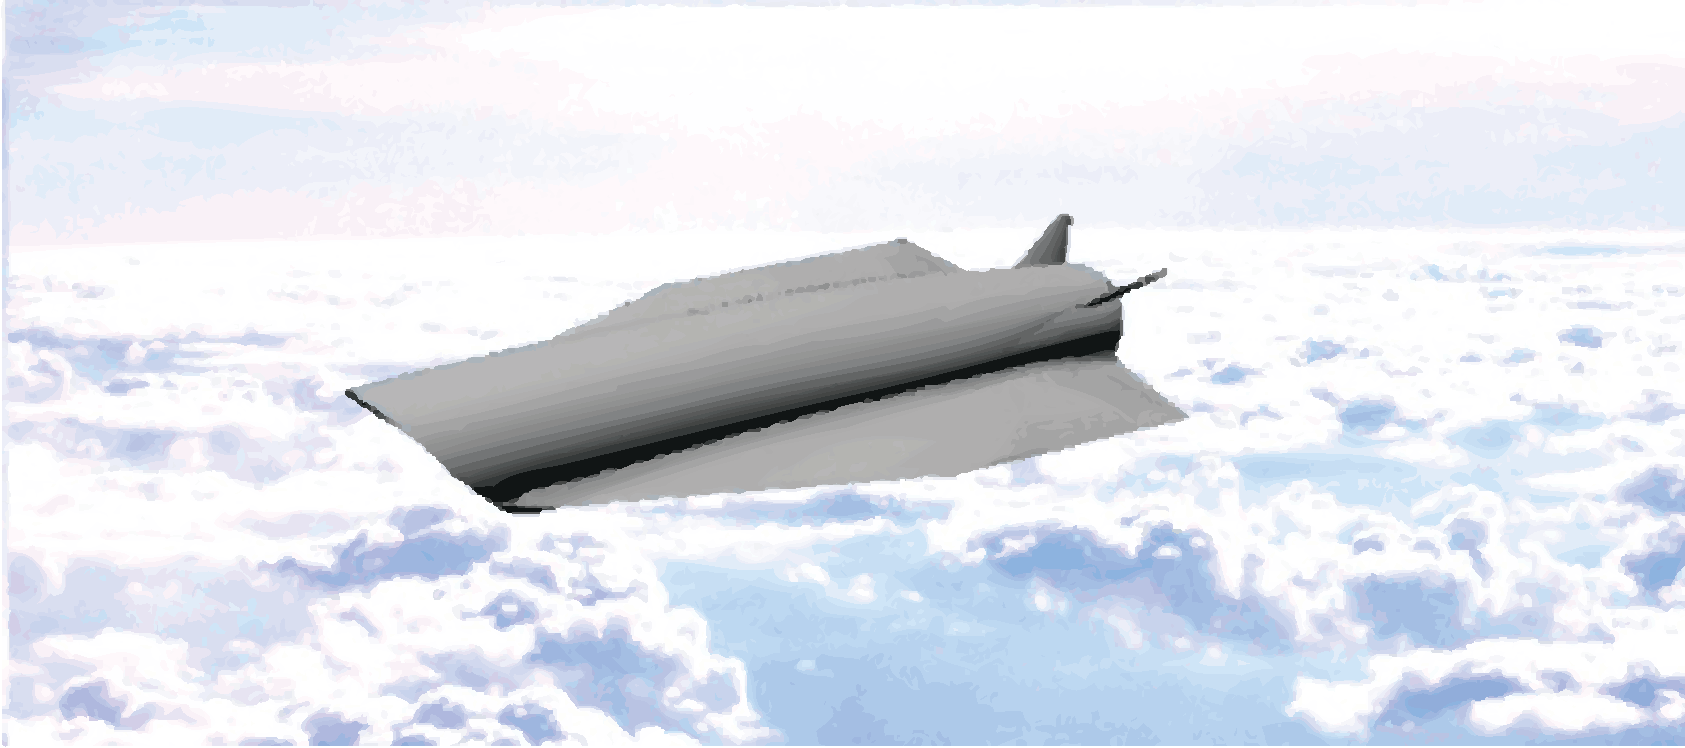
\includegraphics[width=4cm]{../fig/ghvclouds.pdf}};
      \node[squareblock, minimum height=1.5cm, minimum width=4.0cm, above of=block3,node distance=2.25cm] (block4) {\shortstack[c]{Reference\\Model}};
      \node[whitesum,right of=block3, node distance=3.5cm] (sum2) {};
      % \node[coordinate,above of=sum2, node distance=3.5cm] (node_L) {};
      \node[squareblock, minimum height=1.0cm, minimum width=1.0cm, above of=sum2,node distance=3.5cm] (block_L) {$L$};

      \node[input,below of=block2, node distance=1.5cm] (input2) {};
      \node[coordinate,right of=sum2, node distance=1.5cm] (node_output) {};
      \node[output,right of=node_output, node distance=1.5cm] (output1) {};
      \node[coordinate,below of=block3, node distance=2.5cm] (node_feedback) {};
      \node[coordinate,left of=node_feedback, node distance=1.5cm] (node_feedback2) {};
      \node[coordinate,below of=block2, node distance=0.7cm] (node_feedback3) {};

      % Gray shaded box
      \begin{pgfonlayer}{background}
        \path (block1 |- block1)+(-1.5,0.7) node (c) {};
        \path (block2 -| block2)+(1.5,-0.7) node (d) {};
        \path[fill=gray!20, draw] (c) rectangle (d);
      \end{pgfonlayer}

      % Draw
      \draw [vecArrow]  (node_control) -- (block3);
      \draw [vecArrow]  (node_tee1) |- (block4);
      \draw [vecArrow]  (node_input) -- (node_reference);
      \draw [vecArrow]  (block3) -- node [pos=0.7]{$+$} (sum2);
      \draw [vecArrow]  (block4) -| node [pos=0.9]{$-$} (sum2);
      \draw [vecArrow]  (node_output) |- (block_L);
      \draw [vecArrow]  (sum2) -- (output1);
      \draw [vecNoArrow]  (block3) |- (node_feedback2);
      \draw [vecArrow]  (node_feedback2) -| (node_feedback3);
      \draw [vecArrow]  (block_L) -| (block4);

      % \draw [->]  (b1inB) + (-0.5cm,0cm) -> (b1inB);
      % \draw [->]  (b2inA) + (-1cm,0cm) -> (b2inA);
      % \draw [->]  (b2inB) + (-2.0cm,0cm) -> (b2inB);
      % \draw [-]  (b2inB) + (-2.0cm,0cm) |- (input2);
      % \draw[->](block3) --  node[name=yi,pos=0.3]{state} node[pos=0.9]{$+$} (sum2);
      % \draw[-](yi) |- (input2);

      % \draw [-]  (b1inBleft) + (0.0cm,-1.5cm) -- (b1inBleft);
      % \draw [-]  (b2inAleft) + (0.0cm,1.5cm) -- (b2inAleft);
      % \draw[->](block1) -- node[pos=0.7]{$+$} (sum1);
      % \draw[->](block2) -| node[pos=0.9]{$+$} (sum1);
      % \draw[->](sum1) -- node[pos=0.6]{control} (block3);
      % \draw[->](block4) -| node[pos=0.1]{reference} node[pos=0.95]{$-$} (sum2);
      % \draw[->](sum2) -- node[pos=0.4]{error} (output1);
    \end{tikzpicture}
  \end{center}
\end{figure}

  \clearpage
\section*{\currfilename}

\begin{figure}[H]
  \fontsize{10pt}{10pt}\selectfont
  \begin{center}
    \begin{tikzpicture}[auto, scale=1.0, every node/.style={transform shape}, node distance=1.0cm, >=latex']
      \node[squareblock, minimum height=1cm, minimum width=2cm] (block1){\shortstack[c]{Baseline\\Control}};
      \node[squareblock, below of=block1, node distance=1.5cm, minimum height=1cm, minimum width=2cm] (block2){\shortstack[c]{Adaptive\\Augmentation}};

      \node[coordinate,below of=block1, node distance=0.75cm] (node1) {};
      \node[coordinate,right of=node1, node distance=1.5cm] (node_control) {};
      \node[coordinate,left of=node1, node distance=1.5cm] (node_reference) {};
      \node[coordinate, left of=node_reference, node distance=1.5cm] (node_input) {};
      \node[coordinate, right of=node_input, node distance=0.5cm] (node_tee1) {};
      \node[coordinate, below of=block3, node distance=2.5cm] (node_tee2) {};

      \node[right of=node_control,draw=black, node distance=3.5cm, minimum width=2cm, inner sep= 0mm] (block3) {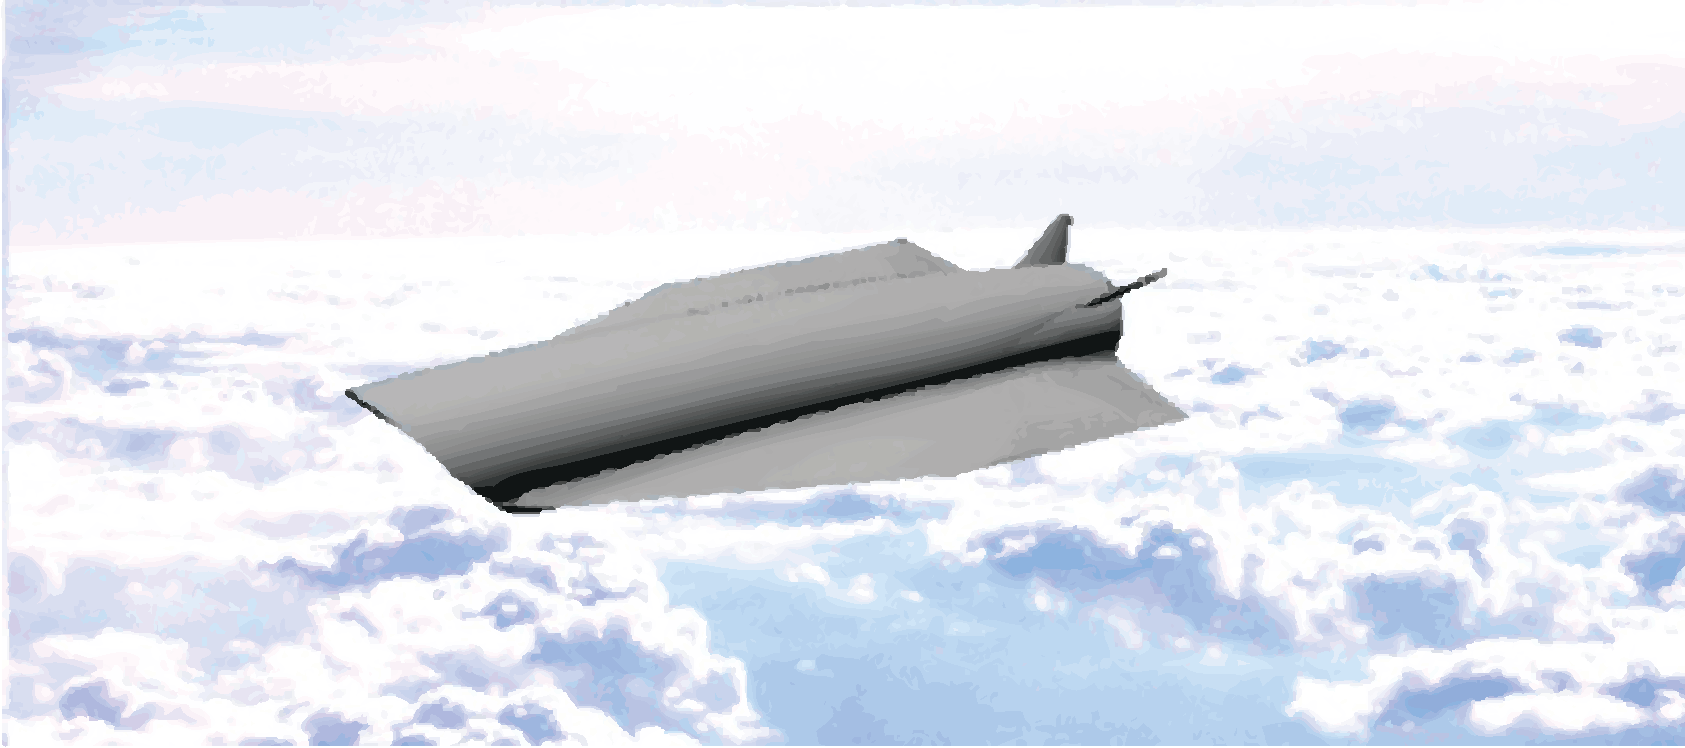
\includegraphics[width=4cm]{../fig/ghvclouds.pdf}};
      \node[squareblock, minimum height=1.5cm, minimum width=4.0cm, above of=block3,node distance=2.25cm] (block4) {\shortstack[c]{Reference\\Model}};
      \node[whitesum,right of=block3, node distance=3.5cm] (sum2) {};
      % \node[coordinate,above of=sum2, node distance=3.5cm] (node_L) {};
      % \node[squareblock, minimum height=1.0cm, minimum width=1.0cm, above of=sum2,node distance=3.5cm] (block_L) {$L$};

      \node[input,below of=block2, node distance=1.5cm] (input2) {};
      \node[coordinate,right of=sum2, node distance=0.25cm] (node_output) {};
      \node[output,right of=node_output, node distance=1.5cm] (output1) {};
      \node[coordinate,below of=block3, node distance=2.5cm] (node_feedback) {};
      \node[coordinate,left of=node_feedback, node distance=1.5cm] (node_feedback2) {};
      \node[coordinate,below of=block2, node distance=0.7cm] (node_feedback3) {};

      % Gray shaded box
      \begin{pgfonlayer}{background}
        \path (block1 |- block1)+(-1.5,0.7) node (c) {};
        \path (block2 -| block2)+(1.5,-0.7) node (d) {};
        \path[fill=gray!20, draw] (c) rectangle (d);
      \end{pgfonlayer}

      % Draw
      \draw [vecArrow]  (node_control) -- (block3);
      \draw [vecArrow]  (node_tee1) |- (block4);
      \draw [vecArrow]  (node_input) -- (node_reference);
      \draw [vecArrow]  (block3) -- node [pos=0.7]{$+$} (sum2);
      \draw [vecArrow]  (block4) -| node [pos=0.9]{$-$} (sum2);
      % \draw [vecArrow]  (node_output) |- (block_L);
      \draw [vecArrow]  (sum2) -- (output1);
      \draw [vecNoArrow]  (block3) |- (node_feedback2);
      \draw [vecArrow]  (node_feedback2) -| (node_feedback3);

      % \draw [vecArrow]  (block_L) -| (block4);
      % \draw [->]  (b1inB) + (-0.5cm,0cm) -> (b1inB);
      % \draw [->]  (b2inA) + (-1cm,0cm) -> (b2inA);
      % \draw [->]  (b2inB) + (-2.0cm,0cm) -> (b2inB);
      % \draw [-]  (b2inB) + (-2.0cm,0cm) |- (input2);
      % \draw[->](block3) --  node[name=yi,pos=0.3]{state} node[pos=0.9]{$+$} (sum2);
      % \draw[-](yi) |- (input2);

      % \draw [-]  (b1inBleft) + (0.0cm,-1.5cm) -- (b1inBleft);
      % \draw [-]  (b2inAleft) + (0.0cm,1.5cm) -- (b2inAleft);
      % \draw[->](block1) -- node[pos=0.7]{$+$} (sum1);
      % \draw[->](block2) -| node[pos=0.9]{$+$} (sum1);
      % \draw[->](sum1) -- node[pos=0.6]{control} (block3);
      % \draw[->](block4) -| node[pos=0.1]{reference} node[pos=0.95]{$-$} (sum2);
      % \draw[->](sum2) -- node[pos=0.4]{error} (output1);
    \end{tikzpicture}
  \end{center}
\end{figure}


  \clearpage
\section*{\currfilename}

\begin{tikzpicture}[x=1mm, y=1mm,>=latex,line join=round,font=\Large,auto, scale=1.0, every node/.style={transform shape}, node distance=1.0cm, >=latex']
  % Place coordinates for everything in the body axes frame that will be rotated
  \begin{scope}[rotate=-20]
    \coordinate (o)       at (0,0);
    \coordinate (A)       at ($(o)+(0,0)$);
    \coordinate (B)       at ($(A)+(70,20)$);
    \coordinate (C)       at ($(B)+(70,-20)$);
    \coordinate (D)       at ($(C)+(-70,-20)$);
    \coordinate (E)       at ($(D)+(-70,20)$);
    \coordinate (center)  at ($(B)+(0,-20)$);
    \coordinate (F)       at ($(center)+(-80,0)$);
    \coordinate (G)       at ($(center)+(80,0)$);
    \coordinate (thrust)  at ($(center)+(-50,0)$);
    \coordinate (cg)      at ($(center)+(-10,0)$);
    \coordinate (cgnew)   at ($(center)+(-30,0)$);
    \coordinate (Fminus)  at ($(center)+(-70,0)$);
  \end{scope}

  % Draw arcs for the angles theta and alpha
  \draw[-,line width=1pt] (Fminus) arc(160:170:70) ;
  \draw[-,line width=1pt] (F) arc(160:180:80);

  % Annotate the angles theta and alpha
  \node at ($(E)+(-4,-5)$) {$\alpha$};
  \node at ($(F)+(-6,-12)$) {$\theta$};

  % Make the points for horizon and weight vectors
  \coordinate (hleft)     at ($(center)+(-80,0)$);
  \coordinate (hright)    at ($(center)+(80,0)$);
  \coordinate (weight)    at ($(cg)+(0,-30)$);
  \coordinate (weightnew) at ($(cgnew)+(0,-30)$);

  % Points that will be rotated for stability axes
  \begin{scope}[rotate=-10]
    \coordinate (alphafront)  at ($(center)+(-80,0)$);
    \coordinate (airvelocity) at ($(center)+(-50,0)$);
    \coordinate (alphaback)   at ($(center)+(80,0)$);
    \coordinate (lift)        at ($(center)+(0,30)$);
    \coordinate (drag)        at ($(center)+(50,0)$);
  \end{scope}

  % Now do the points for CG shift components in stability axes
  \begin{scope}[rotate=-10]
    \coordinate (cosadx)      at ($(center)+({-30*cos(10)},0)$);
    \coordinate (cosadxplus)  at ($(center)+({-30*cos(10)},{10*sin(10)})$);
  \end{scope}

  % Draw
  \draw[line width=1pt] (A)-- (B)-- (C)-- (D)-- (E) --cycle;
  \draw[gray, line width=0.5pt] (F)-- (G) --cycle;
  \draw[gray, line width=0.5pt] (hleft)-- (hright)--cycle;
  \draw[gray, line width=0.5pt] (alphafront)-- (alphaback) --cycle;
  % \draw[gray, line width=0.5pt] (cosadx)-- (cgnew) --cycle;
  % \draw[gray, line width=0.5pt] (cosadxplus)-- (cg) --cycle;
  \draw[->,line width=2pt](center) -- node[pos=0.8]{$L$} (lift);
  \draw[->,line width=2pt](center) -- node[pos=0.8]{$D$} (drag);
  \draw[->,line width=2pt](center) -- node[pos=0.8]{$T$} node[above,pos=0.4]{$\Delta x$} (thrust);
  \draw[->,line width=2pt,gray](cg) -- (weight);
  \draw[->,line width=2pt](cgnew) -- node[pos=0.8]{$W$} (weightnew);
  \draw[->,line width=2pt](alphafront) -- node[pos=0.5]{$V$} (airvelocity);

  % Place original CG location
  \coordinate (CC) at ($(cg)+(2,0)$);
  \coordinate (DD) at ($(cg)+(-2,0)$);
  \filldraw[black,fill=black] (cg)--(CC) arc (360:270:2) -- cycle;
  \filldraw[black,fill=white] (cg)--(CC) arc (0:90:2) -- cycle;
  \filldraw[black,fill=black] (cg)--(DD) arc (180:90:2) -- cycle;
  \filldraw[black,fill=white] (cg)--(DD) arc (180:270:2) -- cycle;
  \draw (cg) circle (2);

  % Place new CG location
  \coordinate (CCnew) at ($(cgnew)+(2,0)$);
  \coordinate (DDnew) at ($(cgnew)+(-2,0)$);
  \filldraw[black,fill=black] (cgnew)--(CCnew) arc (360:270:2) -- cycle;
  \filldraw[black,fill=white] (cgnew)--(CCnew) arc (0:90:2) -- cycle;
  \filldraw[black,fill=black] (cgnew)--(DDnew) arc (180:90:2) -- cycle;
  \filldraw[black,fill=white] (cgnew)--(DDnew) arc (180:270:2) -- cycle;
  \draw (cgnew) circle (2);
\end{tikzpicture}

  \clearpage
\section*{\currfilename}

\begin{tikzpicture}[x=1mm, y=1mm,>=latex,line join=round,font=\Large,auto, scale=1.0, every node/.style={transform shape}, node distance=1.0cm, >=latex']
  %Place coordinates for everything in the body axes frame that will be rotated
  \begin{scope}[rotate=-20]
    \coordinate (o)       at (0,0);
    \coordinate (A)       at ($(o)+(0,0)$);
    \coordinate (B)       at ($(A)+(70,20)$);
    \coordinate (C)       at ($(B)+(70,-20)$);
    \coordinate (D)       at ($(C)+(-70,-20)$);
    \coordinate (E)       at ($(D)+(-70,20)$);
    \coordinate (center)  at ($(B)+(0,-20)$);
    \coordinate (F)       at ($(center)+(-80,0)$);
    \coordinate (G)       at ($(center)+(80,0)$);
    \coordinate (thrust)  at ($(center)+(-50,0)$);
    \coordinate (cg)      at ($(center)+(-10,0)$);
    \coordinate (cgnew)   at ($(center)+(-30,0)$);
    \coordinate (Fminus)  at ($(center)+(-70,0)$);
    \coordinate (yaxis)   at ($(center)+(0,40)$);
  \end{scope}

  % Draw arcs for the angles theta and alpha
  \draw[-,line width=1pt] (Fminus) arc(160:170:70);
  \draw[-,line width=1pt] (F) arc(160:180:80);

  % Annotate the angles theta and alpha
  \node at ($(E)+(-4,-5)$) {$\alpha$};
  \node at ($(F)+(-6,-12)$) {$\theta$};

  % Make the points for horizon and weight vectors
  \coordinate (hleft)     at ($(center)+(-80,0)$);
  \coordinate (hright)    at ($(center)+(80,0)$);
  \coordinate (weight)    at ($(cg)+(0,-30)$);
  \coordinate (weightnew) at ($(cgnew)+(0,-30)$);

  % Points that will be rotated for stability axes
  \begin{scope}[rotate=-10]
  \coordinate (alphafront)      at ($(center)+(-80,0)$);
  \coordinate (alphafrontminus) at ($(center)+(-70,0)$);
  \coordinate (airvelocity)     at ($(center)+(-40,0)$);
  \coordinate (alphaback)       at ($(center)+(80,0)$);
  \coordinate (lift)            at ($(center)+(0,30)$);
  \coordinate (liftplus)        at ($(center)+(0,40)$);
  \coordinate (drag)            at ($(center)+(50,0)$);
  \end{scope}

  % Now do the points for CG shift components in stability axes
  \begin{scope}[rotate=-10]
  \coordinate (cosadx)      at ($(center)+({-30*cos(10)},0)$);
  \coordinate (cosadxplus)  at ($(center)+({-30*cos(10)},{10*sin(10)})$);
  \end{scope}

  % Draw
  \draw[line width=1pt] (A)-- (B)-- (C)-- (D)-- (E) --cycle;
  \draw[->,gray, line width=0.5pt] (G) -- node[above,pos=0.95]{$x_{b}$} (F);
  \draw[->,gray, line width=0.5pt] (center) -- node[right,pos=0.9]{$z_{b}$} (yaxis);
  \draw[gray, line width=0.5pt] (hleft)-- (hright)--cycle;
  \draw[->,gray, line width=0.5pt] (alphaback) -- node[pos=0.95]{$x_{s}$} (alphafront);
  \draw[->,gray,line width=0.5pt](center) -- node[pos=0.9]{$z_{s}$} (liftplus);
  \draw[->,line width=2pt](center) -- node[pos=0.8]{$L$} (lift);
  \draw[->,line width=2pt](center) -- node[pos=0.8]{$D$} (drag);
  \draw[->,line width=2pt](center) -- node[above,pos=0.8]{$T$} (thrust);
  \draw[->,line width=2pt,black](cg) -- node[pos=0.8]{$W$} (weight);
  \draw[->,line width=2pt](alphafrontminus) -- node[below,pos=0.5]{$V$} (airvelocity);

  % Place original CG location
  \coordinate (CC) at ($(cg)+(2,0)$);
  \coordinate (DD) at ($(cg)+(-2,0)$);
  \filldraw[black,fill=black] (cg)--(CC) arc (360:270:2) -- cycle;
  \filldraw[black,fill=white] (cg)--(CC) arc (0:90:2) -- cycle;
  \filldraw[black,fill=black] (cg)--(DD) arc (180:90:2) -- cycle;
  \filldraw[black,fill=white] (cg)--(DD) arc (180:270:2) -- cycle;
  \draw (cg) circle (2);
\end{tikzpicture}

  \clearpage
\section*{\currfilename}

\begin{tikzpicture}[x=1mm, y=1mm,>=latex,line join=round,font=\Large,auto, scale=1.0, every node/.style={transform shape}, node distance=1.0cm, >=latex']
  % Place coordinates for everything in the body axes frame that will be rotated
  \begin{scope}[rotate=-20]
    \coordinate (o)       at (0,0);
    \coordinate (A)       at ($(o)+(0,0)$);
    \coordinate (B)       at ($(A)+(70,20)$);
    \coordinate (C)       at ($(B)+(70,-20)$);
    \coordinate (D)       at ($(C)+(-70,-20)$);
    \coordinate (E)       at ($(D)+(-70,20)$);
    \coordinate (center)  at ($(B)+(0,-20)$);
    \coordinate (F)       at ($(center)+(-80,0)$);
    \coordinate (G)       at ($(center)+(80,0)$);
    \coordinate (thrust)  at ($(center)+(-50,0)$);
    \coordinate (cg)      at ($(center)+(-10,0)$);
    \coordinate (cgnew)   at ($(center)+(-30,0)$);
    \coordinate (Fminus)  at ($(center)+(-70,0)$);
    \coordinate (yaxis)   at ($(center)+(0,40)$);
  \end{scope}

  % Draw arcs for the angles theta and alpha
  \draw[-,line width=1pt] (Fminus) arc(160:170:70);
  \draw[-,line width=1pt] (F) arc(160:180:80);

  % Annotate the angles theta and alpha
  \node at ($(E)+(-4,-5)$) {$\alpha$};
  \node at ($(F)+(-6,-12)$) {$\theta$};

  % Make the points for horizon and weight vectors
  \coordinate (hleft)        at ($(center)+(-80,0)$);
  \coordinate (hright)        at ($(center)+(80,0)$);
  \coordinate (weight)        at ($(cg)+(0,-30)$);
  \coordinate (weightnew)        at ($(cgnew)+(0,-30)$);

  % Points that will be rotated for stability axes
  \begin{scope}[rotate=-10]
    \coordinate (alphafront)      at ($(center)+(-80,0)$);
    \coordinate (alphafrontminus) at ($(center)+(-70,0)$);
    \coordinate (airvelocity)     at ($(center)+(-40,0)$);
    \coordinate (alphaback)       at ($(center)+(80,0)$);
    \coordinate (lift)            at ($(center)+(0,30)$);
    \coordinate (liftplus)        at ($(center)+(0,40)$);
    \coordinate (drag)            at ($(center)+(50,0)$);
  \end{scope}

  % Now do the points for CG shift components in stability axes
  \begin{scope}[rotate=-10]
    \coordinate (cosadx)        at ($(center)+({-30*cos(10)},0)$);
    \coordinate (cosadxplus)        at ($(center)+({-30*cos(10)},{10*sin(10)})$);
  \end{scope}

  % Draw
  \draw[line width=1pt] (A)-- (B)-- (C)-- (D)-- (E) --cycle;
  \draw[->,line width=0.5pt,gray] (G) -- node[above,pos=0.95]{$x_{b}$} (F);
  \draw[->,line width=0.5pt,gray] (center) -- node[right,pos=0.9]{$z_{b}$} (yaxis);
  \draw[gray, line width=0.5pt] (hleft)-- (hright)--cycle;
  \draw[->,gray, line width=0.5pt] (alphaback) -- node[pos=0.95]{$x_{s}$} (alphafront);
  \draw[->,gray,line width=0.5pt](center) -- node[pos=0.9]{$z_{s}$} (liftplus);
  \draw[->,line width=2pt](center) -- node[pos=0.8]{$L$} (lift);
  \draw[->,line width=2pt](center) -- node[pos=0.8]{$D$} (drag);
  \draw[->,line width=2pt](center) -- node[above, pos=0.8]{$T$} node[above,pos=0.4]{$\Delta x$} (thrust);
  \draw[->,line width=2pt](cgnew) -- node[pos=0.8]{$W$} (weightnew);
  \draw[->,line width=2pt](alphafrontminus) -- node[below,pos=0.5]{$V$} (airvelocity);

  % Place original CG location
  \coordinate (CC) at ($(cg)+(2,0)$);
  \coordinate (DD) at ($(cg)+(-2,0)$);
  \filldraw[gray,fill=gray] (cg)--(CC) arc (360:270:2) -- cycle;
  \filldraw[gray,fill=white] (cg)--(CC) arc (0:90:2) -- cycle;
  \filldraw[gray,fill=gray] (cg)--(DD) arc (180:90:2) -- cycle;
  \filldraw[gray,fill=white] (cg)--(DD) arc (180:270:2) -- cycle;
  \draw[gray] (cg) circle (2);

  % Place new CG location
  \coordinate (CCnew) at ($(cgnew)+(2,0)$);
  \coordinate (DDnew) at ($(cgnew)+(-2,0)$);
  \filldraw[black,fill=black] (cgnew)--(CCnew) arc (360:270:2) -- cycle;
  \filldraw[black,fill=white] (cgnew)--(CCnew) arc (0:90:2) -- cycle;
  \filldraw[black,fill=black] (cgnew)--(DDnew) arc (180:90:2) -- cycle;
  \filldraw[black,fill=white] (cgnew)--(DDnew) arc (180:270:2) -- cycle;
  \draw (cgnew) circle (2);
\end{tikzpicture}


  \clearpage
\section*{\currfilename}

\begin{tikzpicture}[scale=1]
  \coordinate (BB) at (0,0);
  \coordinate (CC) at (2,0);
  \coordinate (DD) at (-2,0);
  \filldraw[black,fill=black] (BB)--(CC) arc (360:270:2) -- cycle;
  \filldraw[black,fill=red] (BB)--(CC) arc (0:90:2) -- cycle;
  \filldraw[black,fill=black] (BB)--(DD) arc (180:90:2) -- cycle;
  \filldraw[black,fill=red] (BB)--(DD) arc (180:270:2) -- cycle;
  \draw (BB) circle (2);
\end{tikzpicture}


  \clearpage
\section*{\currfilename}

\begin{figure}[H]
  \fontsize{10pt}{10pt}\selectfont
  \begin{center}
    \begin{tikzpicture}[auto, scale=1.0, every node/.style={transform shape}, node distance=1.0cm, >=latex']
      \node[squareblock, minimum height=2cm, minimum width=1cm] (block1){};
      \matrix[ampersand replacement=\&, row sep=1.2cm, left of=block1,node distance=0.5cm] (block1in) {
        \node [coordinate] (b1inA) {}; \\
        \node [coordinate] (b1inB) {}; \\
      };
      \matrix[ampersand replacement=\&, row sep=1.2cm, right of=block1,node distance=0.5cm] (block1out) {
        \node [coordinate] (b1outA) {}; \\
        \node [coordinate] (b1outB) {}; \\
      };
      \node[input, left of=b1inA,node distance=1.5cm](input1){};
      \node[input, left of=b1inB,node distance=1.5cm](input2){};
      \node[roundblock,right of=b1outA, node distance=1.2cm, minimum height=0.8cm] (block2) {$J$};
      \node[roundblock,right of=b1outB, node distance=1.2cm, minimum height=0.8cm] (block3) {$K$};
      \node[roundblock,below of=block3, node distance=1.2cm, minimum height=0.8cm] (block4) {$B$};
      \node[whitesum,right of=block3, node distance=1.5cm] (sum1) {};
      \node[squareblock, minimum height=1cm, minimum width=2cm, right of=sum1,node distance=2.5cm] (block5) {$\frac{1}{Js+B}$};
      \node[output, right of=block5,node distance=2.0cm] (output1) {};
      \node[output, below of=block4,node distance=1.0cm](output2){};

      \draw[->](input1) -- node[pos=0.2]{$\dot{x}_{d}$} (b1inA);
      \draw[->](input2) -- node[pos=0.2]{$x_{d}$} (b1inB);
      \draw[->](b1outA) -- node[pos=0.5]{$e_{1}$} (block2);
      \draw[->](b1outB) -- node[pos=0.5]{$e_{1}$} (block3);
      \draw[->](block2) -| node[pos=0.9]{$+$}(sum1);
      \draw[->](block3) -- node[pos=0.7]{$+$} (sum1);
      \draw[->](block4) -| node[pos=0.9]{$+$} (sum1);
      \draw[->](sum1) -- node[pos=0.5]{$\tau$} (block5);
      \draw[->](block5) -- node[pos=0.5,name=x]{$x$} (output1);
      \draw[-](x) |- (output2);
      \draw[->](output2) -| node[pos=0.7,name=x2, above]{} (block1);
      \draw[->](x2) |- (block4);
    \end{tikzpicture}
  \end{center}
\end{figure}

  \clearpage
\section*{\currfilename}

\begin{figure}[H]
  \begin{center}
    \begin{tikzpicture}[auto, scale=0.85, every node/.style={transform shape}, node distance=1.0cm, >=latex']
      \node[squareblock, minimum height=1cm, minimum width=2cm] (block1){\shortstack[c]{Baseline\\Controller}};
      \node[squareblock, below of=block1, node distance=1.5cm, minimum height=1cm, minimum width=2cm] (block2){\shortstack[c]{Adaptive\\Controller}};
      \matrix[ampersand replacement=\&, row sep=0.5cm, left of=block1,node distance=1cm] (block1in) {
        \node [coordinate] (b1inA) {}; \\
        \node [coordinate] (b1inB) {}; \\
      };
      \matrix[ampersand replacement=\&, row sep=0.5cm, left of=block2,node distance=1cm] (block2in) {
        \node [coordinate] (b2inA) {}; \\
        \node [coordinate] (b2inB) {}; \\
      };
      \node [left of=b2inB, node distance=0.5cm] (2B) {};
      \node [below of=2B, node distance=0.12cm] (2B2) {};
      \node [left of=b2inA, node distance=1.0cm] (2A) {};
      \node [below of=2A, node distance=0.12cm] (2A2) {};
      \node[whitesum,right of=block1, node distance=2.5cm] (sum1) {};
      %\node[squareblock, minimum height=1cm, minimum width=2cm, right of=sum1,node distance=2.5cm] (block3) {Actuators};
      \node[squareblock, minimum height=1cm, minimum width=1.0cm, label=below:{\shortstack[c]{Actuator\\Dynamics}}, right of=sum1,node distance=2.5cm, inner sep= 1mm] (block3) {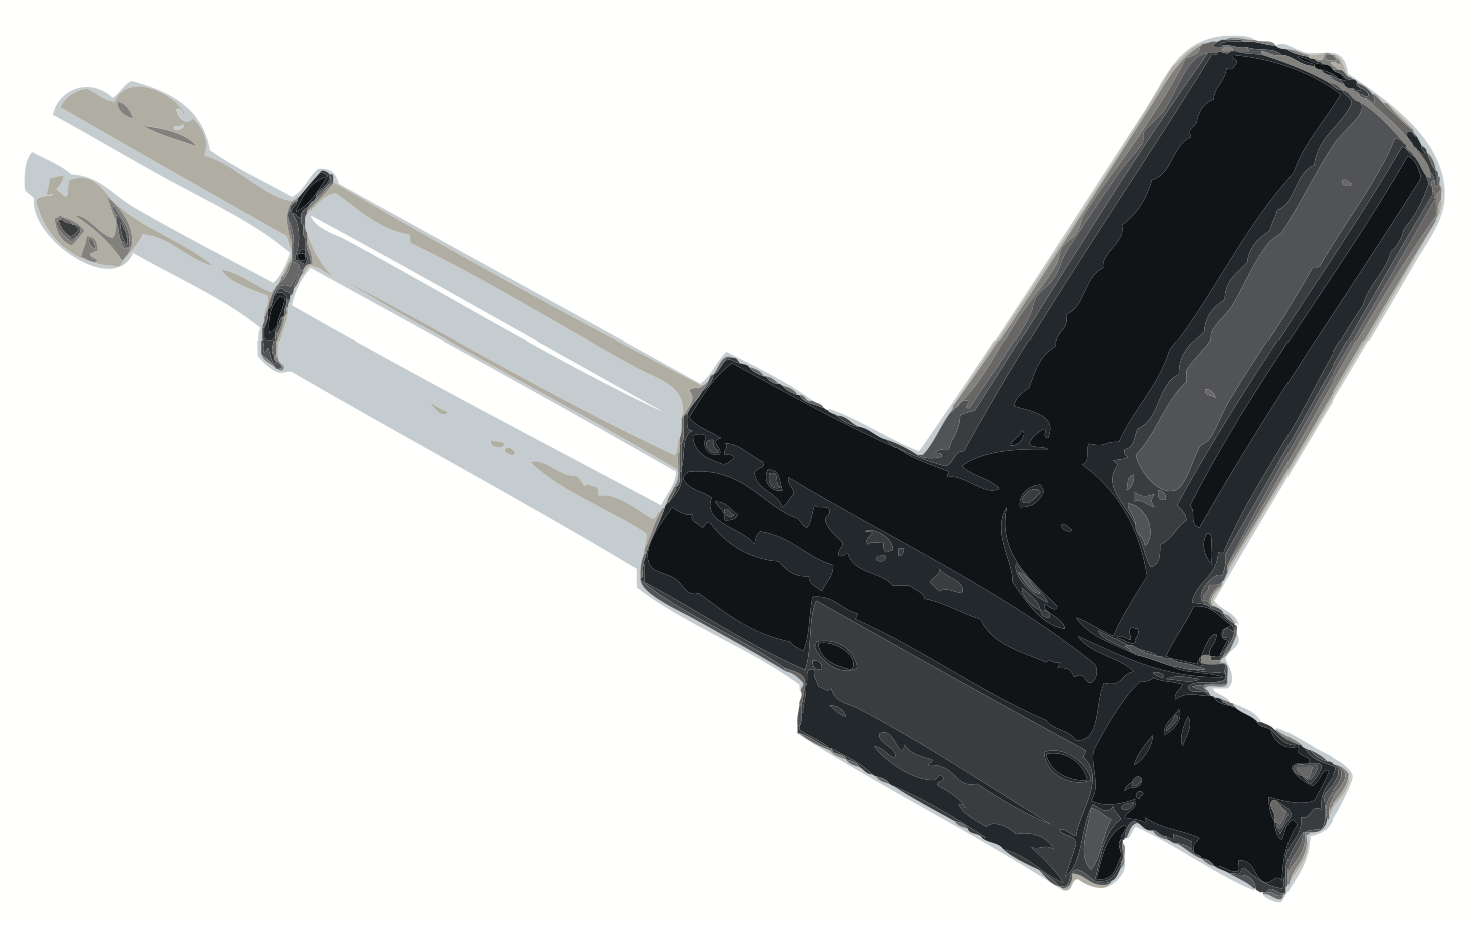
\includegraphics[width=1.6cm]{../fig/actuator_image.png}};
      %\node[squareblock, minimum height=1cm, minimum width=2cm, right of=block3,node distance=3.0cm] (block4) {Plant};
      \node [right of=block3,draw=black, label=below:{\shortstack[c]{6-DOF Nonlinear \\ Equations of Motion}}, anchor=west,node distance=2.0cm, minimum width=2cm, inner sep= 0mm] (block4) {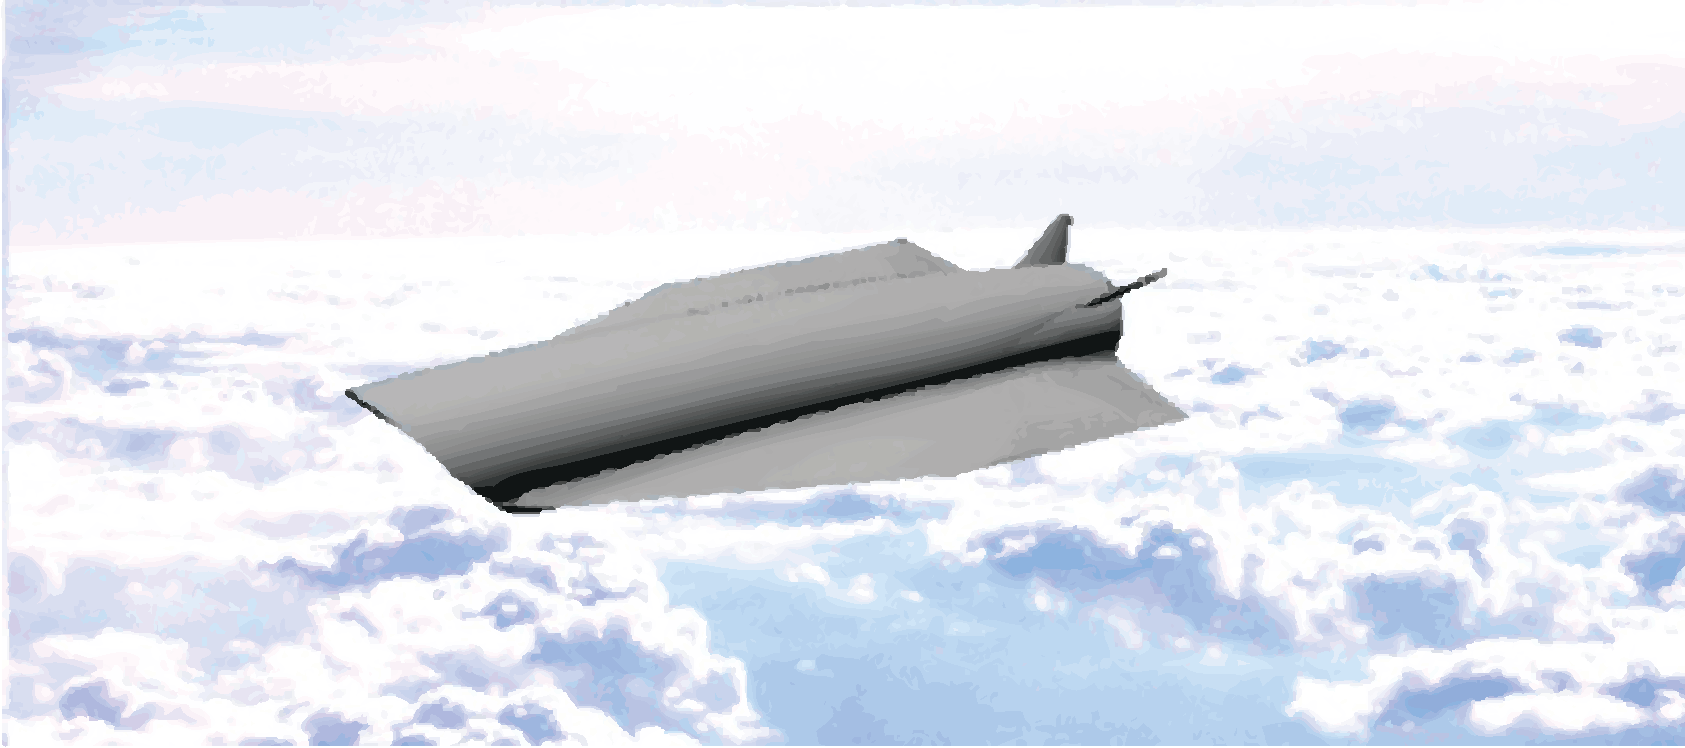
\includegraphics[width=4cm]{../fig/ghvclouds.pdf}};
      %\node[squareblock, minimum height=1cm, minimum width=2cm, right of=block4,node distance=4.0cm] (block5) {Sensors};
      \node[output, right of=block4,node distance=3.5cm] (output1) {};
      \node[input, below of=block2,node distance=1.5cm](input2){};

      \draw [->]  (b1inA) + (-2.5cm,0cm) -> node [pos=0.15]{$z_{\text{cmd}}$}  (b1inA);
      \draw [->]  (b1inB) + (-0.5cm,0cm) -> (b1inB);
      \draw [->]  (b2inA) + (-1cm,0cm) -> (b2inA);
      \draw [->]  (b2inB) + (-2.0cm,0cm) -> node[name=TB,node distance=2.5cm]{} (b2inB);
      \draw[->](block4) --  node[name=yi,pos=0.4]{}(output1);
      \draw[-](yi) |- (input2);
      \draw[-](b1inB) + (-0.5cm,0cm) -- (2B2);
      \draw[-](b1inA) + (-1.0cm,0cm) -- (2A2) ;
      \draw[-] (b2inB) + (-2.0cm,0cm) |- (input2);
      \draw[->](block1) -- node[pos=0.22]{$u_{\text{bl}}$} node[pos=0.9]{$+$} (sum1);
      \draw[->](block2) -| node[pos=0.1]{$u_{\text{ad}}$} node[pos=0.9]{$+$} (sum1);
      \draw[->](sum1) -- (block3);
      \draw[->](block3) -- (block4);
      % \draw[->](block4) -- (block5);
      \begin{pgfonlayer}{background}
        \path (block1 |- block1)+(-2.5,0.7) node (c) {};
        \path (block2 -| block2)+(3.0,-0.7) node (d) {};
        \path[fill=gray!20, draw, dashed] (c) rectangle (d);
      \end{pgfonlayer}
      % \node [below of=block2, node distance = 0.9cm] {Controller};
    \end{tikzpicture}
    \caption{Baseline plus adaptive control block diagram \label{fig.baseplusadaptiveblock}}
  \end{center}
\end{figure}

  \clearpage
\section*{\currfilename}

\begin{figure}[H]
  \fontsize{14pt}{14pt}\selectfont
  \begin{center}
    \begin{tikzpicture}[auto, scale=1.0, every node/.style={transform shape}, node distance=0.1cm, >=latex']
      \node[squareblock, minimum height=2cm, minimum width=1cm] (block1){};

      \matrix[ampersand replacement=\&, row sep=0.8cm, left of=block1,node distance=0.5cm] (block1in) {
        \node [coordinate] (b1inA) {}; \\
        \node [coordinate] (b1inB) {}; \\
      };

      \matrix[ampersand replacement=\&, row sep=0.8cm, right of=block1,node distance=0.5cm] (block1out) {
        \node [coordinate] (b1outA) {}; \\
        \node [coordinate] (b1outB) {}; \\
      };

      \node[input, left of=b1inA,node distance=1.5cm](input1){};
      \node[input, left of=b1inB,node distance=1.5cm](input2){};
      \node[roundblock,right of=b1outA, node distance=1.2cm, minimum height=0.8cm] (block2) {$J$};
      \node[roundblock,right of=b1outB, node distance=1.2cm, minimum height=0.8cm] (block3) {$K$};
      \node[roundblock,below of=block3, node distance=1.2cm, minimum height=0.8cm] (block4) {$B$};
      \node[output,left of=block4, node distance=1.7cm](nodeB){};
      \node[whitesum,right of=block3, node distance=1.5cm] (sum1) {};
      \node[squareblock, minimum height=1cm, minimum width=2cm, right of=sum1,node distance=2.5cm] (block5) {$\dsp{\frac{1}{s(Js+B)}}$};
      \node[output, right of=block5,node distance=3.5cm] (output1) {};
      \node[output, below of=block4,node distance=1.0cm](output2){};

      \draw[->](input1) -- node[pos=0.2]{$\ddot{x}_{d}$} (b1inA);
      \draw[->](input2) -- node[pos=0.2]{$x_{d}$} (b1inB);
      \draw[->](b1outA) -- node[pos=0.5]{$e_{1}$} (block2);
      \draw[->](b1outB) -- node[pos=0.5]{$e_{2}$} (block3);
      \draw[->](block2) -| node[pos=0.9]{$+$}(sum1);
      \draw[->](block3) -- node[pos=0.7]{$+$} (sum1);
      \draw[->](block4) -| node[pos=0.9]{$+$} (sum1);
      \draw[->](sum1) -- node[pos=0.5]{$\tau$} (block5);
      \draw[->](block5) -- node[pos=0.5,name=x]{} (output1);
      \draw[vecNoArrow](x) |- (output2);
      \draw[vecArrow](output2) -| (nodeB);
      \draw[->](nodeB) -| node[pos=0.9]{$x$} (block1);
      \draw[->](nodeB) |- node[pos=0.9]{$\dot{x}$} (block4);
    \end{tikzpicture}
  \end{center}
\end{figure}


  \clearpage
\section*{\currfilename}

\begin{tikzpicture}[x         = 1mm,
                    y         = 1mm,
                    >         = latex,
                    line join = round,
                    font      = \small]

  %%%%%%%%%%%%%%%%%%
  % NOZZLE DRAWING %
  %%%%%%%%%%%%%%%%%%
  %-> Origin definition
  \coordinate (o) at (0,0);

  %-> Nozzle
  % Symmetric characteristic is used in a
  % foreach command where the cycle is made
  % for upper part (up) with positive sign (+)
  % and lower part (down) with negative sign (-)
  \foreach \pos/\sign in {up/+,down/-}{

  %%-> Points definitions
  \coordinate (A\pos)        at ($(o)+(0,\sign11.5)$);
  \coordinate (B\pos)        at ($(A\pos)+(0,\sign5.075)$);
  \coordinate (C\pos)        at ($(B\pos)+(20,0)$);
  \coordinate (D\pos)        at ($(C\pos)+(0,-\sign1.575)$);
  \coordinate (E\pos)        at ($(D\pos)+(10,0)$);
  \coordinate (F\pos)        at ($(E\pos)+(0,\sign11)$);
  \coordinate (G\pos)        at ($(F\pos)+(0,\sign8)$);
  \coordinate (H\pos)        at ($(G\pos)+(0,\sign6)$);
  \coordinate (I\pos)        at ($(H\pos)+(10,0)$);
  \coordinate (L\pos)        at (G\pos-|I\pos);
  \coordinate (M\pos)        at (F\pos-|I\pos);
  \coordinate (N\pos)        at (E\pos-|I\pos);
  \coordinate (O\pos)        at ($(N\pos)+(100,0)$);
  \coordinate (P\pos)        at ($(O\pos)+(10,-\sign10)$);
  \coordinate (throat_\pos)  at ($(P\pos)-(43.8,\sign1.15)$);
  \coordinate (IN_\pos)      at ($(A\pos)+(92.74,0)$);
  \coordinate (center1_\pos) at ($(o)+(92.74,\sign4.5)$);
  \coordinate (center2_\pos) at ($(throat_\pos)+(0,\sign7)$);

  %%-> Draw nozzle main body
  \draw[fill,
        pattern    = section,
        line width = 1.1pt]
  \ifnum\sign1>0
          (center1_\pos)++(45:7)arc(45:90:7)--
  \else
          (center1_\pos)++(-45:7)arc(315:270:7)--
  \fi
  (A\pos)--
  (B\pos)--
  (C\pos)--
  (D\pos)--
  (E\pos)--
  (F\pos)--
  (G\pos)--
  (H\pos)--
  (I\pos)--
  (L\pos)--
  (M\pos)--
  (N\pos)--
  (O\pos)--
  (P\pos)--
  (throat_\pos)
  \ifnum\sign1>0
        arc(270:225:7)
  \else
       arc(90:135:7)
  \fi
  --cycle;

  %%-> Draw holes on the flange
  \draw[fill       = white,
        line width = 1.1pt] (G\pos)rectangle(M\pos);

  %%-> Draw symmetric axis on flange holes
  \draw[dash pattern = on 3pt off 5pt on 6pt off 5pt,
        line width   = 1pt] ($(F\pos)!.5!(G\pos)-(5,0)$)--
                            ($(L\pos)!.5!(M\pos)+(5,0)$);

  %%-> screw drawing
  \draw[dashed] (D\pos)--(D\pos-|A\pos);
  }

  %%-> Nozzle input and output closure
  \draw[line width = 1.1pt](Adown)--(Aup)
                           (Pdown)--(Pup);

  %%-> Nozzle symmetry line
  \draw[dash pattern = on 3pt off 5pt on 6pt off 5pt,
        line width   = 1pt] ($(Adown)!.5!(Aup)-(5,0)$)--($(Pdown)!.5!(Pup)+(5,0)$);

  %%%%%%%%%%%%%%
  % DIMENSIONS %
  %%%%%%%%%%%%%%
  % Macro to see the dimension
  % inserted. For debug.
  \newif\ifdimension
  \dimensionfalse
  %\dimensiontrue % if true, you will see the dimension number (%x) on the draw
  \newcount\Ndim=0
  \def\SeeDim#1{\ifdimension\global\advance\Ndim by 1 \the\Ndim\else#1\fi}
  %-> 1
  \Hdimension[text      = \SeeDim{10},
              distance  = 3]  (Hup) --  (Iup);

  %-> 2
  \Hdimension[text     = \SeeDim{10},
              distance = 3] (Cup)--(Hup);

  %-> 3
  \Hdimension[text     = \SeeDim{20},
              distance = 26.425] (Bup)--(Cup);

  %-> 4
  \Hdimension[text     = \SeeDim{100},
              distance = 3] (Iup)--(Oup);

  %-> 5
  \Hdimension[text     = \SeeDim{10},
              distance = 28] (Oup)--(Pup);

  %-> 6
  \dimension[text     = \SeeDim{\diameter30},
             distance = -25] (Odown)--(Oup);

  %-> 7
  \Hdimension[text     = \SeeDim{43.8},
              distance = -48.15] (throat_down)--(Odown);

  %-> 8
  \Hdimension[text     = \SeeDim{92.74},
              distance = -40.5] (IN_down)--(Bdown);

  %-> 9
  \dimension[text             = \SeeDim{\diameter7.7},
             text translation = -7mm,
             distance         = 20] (throat_down)--(throat_up);

  %-> 10
  \dimension[text     = \SeeDim{\diameter10},
             distance = -8] (Pdown)--(Pup);

  %-> 11 (by hand)
  \draw[->] (center1_up)--++(45:7)node[sloped,
                                       above     = .4mm,
                                       pos       = .3,
                                       inner sep = 0.5pt]{\SeeDim{R7}};

  %-> 12 (by hand)
  \draw[->] (center2_up)--++(225:7)node[above     = .4mm,
                                        pos       = .4,
                                        inner sep = 0.5pt,
                                        rotate    = 45,
                                        fill      = white]{\SeeDim{R7}};

  %-> 13 (by hand)
  \coordinate (raccordo_up)   at ($(center1_up)+(45:7)$);
  \coordinate (raccordo_down) at ($(center1_down)+(-45:7)$);
  \draw (raccordo_up)--++(135:20);
  \draw (raccordo_down)--++(225:20);
  \path[name path=C1](raccordo_up)--++(-45:20);
  \path[name path=C2](raccordo_down)--++(45:20);
  \path[name intersections={of=C1 and C2}];
  \coordinate (C90) at (intersection-1);
  \draw[<->] ($(C90)+(135:30)$)arc[start angle = 135,
                                   delta angle = 90,
                                   radius      = 30];
  \def\angle{35}
  \node[rotate = \angle+45,
        anchor = south] at ($(C90)+(135+\angle:30)$){\SeeDim{\ang{90}}};

  %-> 14
  \dimension[text             = \SeeDim{\diameter60},
             distance         = -5,
             >                = angle 45,
             text translation = .5cm] ($(Ldown)!.5!(Mdown)$)--($(Lup)!.5!(Mup)$);

  %-> 15
  \dimension[text             = \SeeDim{\diameter80},
             distance         = -10,
             text translation = .5cm] (Idown)--(Iup);

  %-> 16
  \dimension[text             = \SeeDim{\diameter8 ($\times$4)},
             distance         = 10,
             text translation = -12mm] (Gdown)--(Fdown);

  %-> 17
  \dimension[text     = \SeeDim{G1'},
             distance = 10] (Bdown)--(Bup);

  %-> 18
  \dimension[text     = \SeeDim{\diameter23},
             distance = 5] (Adown)--(Aup);

  % Dimensions scale
  \node[anchor = north west] at (current bounding box.south west)
  {All dimensions are in millimeters};
\end{tikzpicture}

  \clearpage
\section*{\currfilename}

\begin{tikzpicture}[x=1mm, y=1mm,>=latex,line join=round,font=\small]
  \coordinate (o) at (0,0);
  \coordinate (A) at ($(o)+(0,0)$);
  % \coordinate (B) at ($(A)+(165,0)$); %for 1in margins
  \coordinate (B) at ($(A)+(152,0)$); %for 1.25in margins
  \coordinate (C) at ($(B)+(0,-20)$);
  \coordinate (D) at ($(C)+(-50,0)$);
  \coordinate (E) at ($(D)+(-16,6)$);
  \coordinate (F) at ($(E)+(-12,3)$);
  \coordinate (G) at ($(C)+(0,-10)$);
  \coordinate (H) at ($(G)+(-70,0)$);
  \coordinate (I) at ($(H)+(20,-6)$);
  \coordinate (L) at ($(G)+(0,-6)$);

  \draw[fill, pattern=section, line width=1.1pt]
  (A)--
  (B)--
  (C)--
  (D)--
  (E)--
  (F)--
  (A)
  --cycle;

  \draw[fill, pattern=section, line width=1.1pt]
  (G)--
  (H)--
  (I)--
  (L)
  --cycle;

  \newif\ifdimension
  \dimensionfalse
  %\dimensiontrue % if true, you will see the dimension number (%x) on the draw
  \newcount\Ndim=0
  \def\SeeDim#1{\ifdimension\global\advance\Ndim by 1 \the\Ndim\else#1\fi}
  \Hdimension[text=\SeeDim{10}, distance=-40]  (A)--(B);

  %%-> 2
  %\Hdimension[text=\SeeDim{10}, distance=3] (Cup)--(Hup);
  %
  %%-> 3
  %\Hdimension[text=\SeeDim{20}, distance=26.425] (Bup)--(Cup);
  %%-> 4
  %\Hdimension[text     = \SeeDim{100},
  %            distance = 3] (Iup)--(Oup);
  %
  %%-> 5
  %\Hdimension[text     = \SeeDim{10},
  %            distance = 28] (Oup)--(Pup);
  %
  %%-> 6
  %\dimension[text     = \SeeDim{\diameter30},
  %           distance = -25] (Odown)--(Oup);
  %
  %%-> 7
  %\Hdimension[text     = \SeeDim{43.8},
  %            distance = -48.15] (throat_down)--(Odown);
  %
  %%-> 8
  %\Hdimension[text     = \SeeDim{92.74},
  %            distance = -40.5] (IN_down)--(Bdown);
  %
  %%-> 9
  %\dimension[text             = \SeeDim{\diameter7.7},
  %           text translation = -7mm,
  %           distance         = 20] (throat_down)--(throat_up);
  %
  %%-> 10
  %\dimension[text     = \SeeDim{\diameter10},
  %           distance = -8] (Pdown)--(Pup);
  %
  %%-> 11 (by hand)
  %\draw[->] (center1_up)--++(45:7)node[sloped,
  %                                     above     = .4mm,
  %                                     pos       = .3,
  %                                     inner sep = 0.5pt]{\SeeDim{R7}};
  %
  %%-> 12 (by hand)
  %\draw[->] (center2_up)--++(225:7)node[above     = .4mm,
  %                                      pos       = .4,
  %                                      inner sep = 0.5pt,
  %                                      rotate    = 45,
  %                                      fill      = white]{\SeeDim{R7}};
  %
  %%-> 13 (by hand)
  %\coordinate (raccordo_up)   at ($(center1_up)+(45:7)$);
  %\coordinate (raccordo_down) at ($(center1_down)+(-45:7)$);
  %\draw (raccordo_up)--++(135:20);
  %\draw (raccordo_down)--++(225:20);
  %\path[name path=C1](raccordo_up)--++(-45:20);
  %\path[name path=C2](raccordo_down)--++(45:20);
  %\path[name intersections={of=C1 and C2}];
  %\coordinate (C90) at (intersection-1);
  %\draw[<->] ($(C90)+(135:30)$)arc[start angle = 135,
  %                                 delta angle = 90,
  %                                 radius      = 30];
  %\def\angle{35}
  %\node[rotate = \angle+45,
  %      anchor = south] at ($(C90)+(135+\angle:30)$){\SeeDim{\ang{90}}};
  %
  %%-> 14
  %\dimension[text             = \SeeDim{\diameter60},
  %           distance         = -5,
  %           >                = angle 45,
  %           text translation = .5cm] ($(Ldown)!.5!(Mdown)$)--($(Lup)!.5!(Mup)$);
  %
  %%-> 15
  %\dimension[text             = \SeeDim{\diameter80},
  %           distance         = -10,
  %           text translation = .5cm] (Idown)--(Iup);
  %
  %%-> 16
  %\dimension[text             = \SeeDim{\diameter8 ($\times$4)},
  %           distance         = 10,
  %           text translation = -12mm] (Gdown)--(Fdown);
  %
  %%-> 17
  %\dimension[text     = \SeeDim{G1'},
  %           distance = 10] (Bdown)--(Bup);
  %
  %%-> 18
  %\dimension[text     = \SeeDim{\diameter23},
  %           distance = 5] (Adown)--(Aup);
  %% Dimensions scale
  %\node[anchor = north west] at (current bounding box.south west){All dimensions are in millimeters};

\end{tikzpicture}

  \clearpage
\section*{\currfilename}

\begin{tikzpicture}[x=1mm, y=1mm,>=latex,line join=round,font=\small]
  \coordinate (o) at (0,0);

  % Upper part
  \coordinate (A) at ($(o)+(0,0)$);
  \coordinate (B) at ($(A)+(152,0)$);
  \coordinate (C) at ($(B)+(-35,-12)$);
  \coordinate (D) at ($(C)+(-35,0)$);
  \coordinate (E) at ($(D)+(-16,6)$);
  \coordinate (F) at ($(E)+(-12,3)$);

  % Lower part
  \coordinate (G) at ($(C)+(28,-10)$);
  \coordinate (H) at ($(G)+(-30,-2)$);
  \coordinate (I) at ($(H)+(-35,0)$);
  \coordinate (J) at ($(I)+(-15,5)$);
  \coordinate (K) at ($(J)+(12,-7)$);
  \coordinate (L) at ($(K)+(30,-1)$);

  % Draw top
  \draw[fill, pattern=section, line width=1.1pt]
  (A)--
  (B)--
  (C)--
  (D)--
  (E)--
  (F)--
  (A)
  --cycle;

  % Draw bottom
  \draw[fill, pattern=section, line width=1.1pt]
  (G)--
  (H)--
  (I)--
  (J)--
  (K)--
  (L)--
  (G)
  --cycle;

  % Dimensions
  \newif\ifdimension
  \dimensionfalse
  \newcount\Ndim=0
  \def\SeeDim#1{\ifdimension\global\advance\Ndim by 1 \the\Ndim\else#1\fi}
  \Hdimension[text=\SeeDim{Inlet}, distance=-40]  (A)--(D);
  \Hdimension[text=\SeeDim{Isolator}, distance=-28]  (D)--(H);
  \Hdimension[text=\SeeDim{Combustor}, distance=-28]  (H)--(C);
  \Hdimension[text=\SeeDim{Nozzle}, distance=-40]  (C)--(B);
\end{tikzpicture}

  \clearpage
\section*{\currfilename}

\begin{tikzpicture}[x=1mm, y=1mm,>=latex,line join=round,font=\small]
  \coordinate (o) at (0,0);

  % Upper part
  \coordinate (A) at ($(o)+(0,0)$);
  \coordinate (B) at ($(A)+(152,0)$);
  \coordinate (C) at ($(B)+(-35,-12)$);
  \coordinate (D) at ($(C)+(-35,0)$);
  \coordinate (E) at ($(D)+(-16,6)$);
  \coordinate (F) at ($(E)+(-12,3)$);

  % Lower part
  \coordinate (G) at ($(C)+(28,-10)$);
  \coordinate (H) at ($(G)+(-45,2)$);
  \coordinate (I) at ($(H)+(-25,0)$);
  \coordinate (J) at ($(I)+(-10,2)$);
  \coordinate (K) at ($(J)+(12,-4)$);
  \coordinate (L) at ($(K)+(30,-1)$);

  % Draw top
  \draw[fill, pattern=section, line width=1.1pt]
  (A)--
  (B)--
  (C)--
  (D)--
  (E)--
  (F)--
  (A)
  --cycle;

  % Draw bottom
  \draw[fill, pattern=section, line width=1.1pt]
  (G)--
  (H)--
  (I)--
  (J)--
  (K)--
  (L)--
  (G)
  --cycle;

  % Shock lines
  \draw[red,ultra thick] (A) -- ($(J)+(6,-6)$);
  \draw[red,ultra thick] (J) -- ($(D)+(-8,3)$);
  \draw[red,ultra thick] ($(D)+(-8,3)$) -- ($(I)+(12,0)$);
  \draw[red,ultra thick] (I) -- ($(D)+(6,0)$);

  % Dimensions
  \newif\ifdimension
  \dimensionfalse
  \newcount\Ndim=0
  \def\SeeDim#1{\ifdimension\global\advance\Ndim by 1 \the\Ndim\else#1\fi}
  \Hdimension[text=\SeeDim{Inlet}, distance=-40]  (A)--(D);
  \Hdimension[text=\SeeDim{Isolator}, distance=-28]  (D)--(H);
  \Hdimension[text=\SeeDim{Combustor}, distance=-28]  (H)--(C);
  \Hdimension[text=\SeeDim{Nozzle}, distance=-40]  (C)--(B);
\end{tikzpicture}

  \clearpage
\section*{\currfilename}

\begin{tikzpicture}[x=1mm, y=1mm,>=latex,line join=round,font=\small]
  \coordinate (o) at (0,0);

  % Upper part
  \coordinate (A) at ($(o)+(0,0)$);
  \coordinate (B) at ($(A)+(152,0)$);
  \coordinate (C) at ($(B)+(-35,-12)$);
  \coordinate (D) at ($(C)+(-35,0)$);
  \coordinate (E) at ($(D)+(-16,4)$);

  % Lower part
  \coordinate (G) at ($(C)+(28,-10)$);
  \coordinate (H) at ($(G)+(-45,2)$);
  \coordinate (I) at ($(H)+(-25,0)$);
  \coordinate (J) at ($(I)+(-10,2)$);
  \coordinate (K) at ($(J)+(12,-4)$);
  \coordinate (L) at ($(K)+(30,-1)$);

  % Draw top
  \draw[fill, pattern=section, line width=1.1pt]
  (A)--
  (B)--
  (C)--
  (D)--
  (E)--
  (A)
  --cycle;

  % Draw bottom
  \draw[fill, pattern=section, line width=1.1pt]
  (G)--
  (H)--
  (I)--
  (J)--
  (K)--
  (L)--
  (G)
  --cycle;

  % Shock lines
  % \draw[red,ultra thick] (A) -- ($(J)+(6,-6)$);
  \draw[red,ultra thick] (A) -- ($(J)+(-30,-6)$);
  \draw[red,ultra thick] (J) -- ($(J)+(-66,8)$);
  % \draw[red,ultra thick] (J) -- ($(J)+(-66,8)$);
  % \draw[red,ultra thick] (J) -- ($(D)+(-8,3)$);
  % \draw[red,ultra thick] ($(D)+(-8,3)$) -- ($(I)+(12,0)$);
  % \draw[red,ultra thick] (I) -- ($(D)+(6,0)$);

  % Dimensions
  % \newif\ifdimension
  % \dimensionfalse
  % \newcount\Ndim=0
  % \def\SeeDim#1{\ifdimension\global\advance\Ndim by 1 \the\Ndim\else#1\fi}
  % \Hdimension[text=\SeeDim{Inlet}, distance=-40]  (A)--(D);
  % \Hdimension[text=\SeeDim{Isolator}, distance=-28]  (D)--(H);
  % \Hdimension[text=\SeeDim{Combustor}, distance=-28]  (H)--(C);
  % \Hdimension[text=\SeeDim{Nozzle}, distance=-40]  (C)--(B);
\end{tikzpicture}


  \clearpage
\section*{\currfilename}

\begin{minipage}{\linewidth}
  \centering
  \begin{tikzpicture}[scale=1]
    \begin{axis}[ axis lines=left,
      xmin=-.1, xmax=1.9,   ymin=-1, ymax=22,
      xlabel={$v$},         ylabel={$p$},
      xtick =\empty,        ytick=\empty,
    ]
      % Compression (Work in)
      \addplot[blue, domain=0.85:0.1,    samples = 20, postaction={decorate},
        decoration={markings, mark=at position 0.6 with {\arrow{>}}}
      ]
      { (0.85/x)^(1.4) }
        [sloped, font=\small]
        node[below, pos=0.7,yshift=-3pt] {$s =$ const.} node[above,pos=0.15,anchor=south west] (L) {};

      % Heat addition
      \addplot[ red, postaction={decorate},
        decoration={markings, mark=at position 0.65 with {\arrow{>}}}
      ]
      coordinates{ (0.1,20) (0.2,20)}
        [ every node/.style={font=\small, text = black} ]
        node[ left, pos = 0] {2}
        node[right, pos = 1] {3};

      % Expansion (Work out)
      \addplot[ blue,domain=0.2:1.7, samples = 40, postaction={decorate},
        decoration={markings, mark=at position 0.32 with {\arrow{>}}}
      ]
      { (1.7/x)^(1.4) }
        [sloped, font=\small]
        node[above, pos=0.3,yshift=5pt] {$s =$ const.} node[above,pos=0.7,anchor=south west] (M) {};

      % Heat removal
      \addplot[ red, postaction={decorate},
        decoration={markings, mark=at position 0.6 with {\arrow{>}}}
      ]
      coordinates{ (1.7,1) (0.85,1) }
        [ every node/.style={font=\small, text = black} ]
        node[below, pos = 0] {4}
        node[below, pos = 1] {1};

      \draw[-latex,blue,line width = 1pt,shorten >= -5pt,shorten <=-5pt]
        (M.south west) -- (M.north west) node[anchor = west, font=\footnotesize,xshift=3pt] {$\dot{W}_{\textrm{out}}$};

      \draw[-latex,blue,line width = 1pt,shorten >= -5pt,shorten <=-5pt]
          (L.south west) node[anchor = east, font=\footnotesize,xshift=-3pt] {$\dot{W}_{\textrm{in}}$} -- (L.north west);
    \end{axis}
  \end{tikzpicture}
  \captionof{figure}{Ideal Brayton cycle}
\end{minipage}

  \clearpage
\section*{\currfilename}

\begin{minipage}{\linewidth}

  \centering
  \begin{tikzpicture}[scale=1]
    \begin{axis}[axis lines=left, xmin=-.1, xmax=1.9, ymin=-1, ymax=22, xlabel={$v$}, ylabel={$p$}, xtick =\empty, ytick=\empty,]
      % Compression
      \addplot[black, domain=0.85:0.1, samples = 20, postaction={decorate},decoration={markings, mark=at position 0.6 with {\arrow{>}}}]
      { (0.85/x)^(1.4) }[sloped, font=\small]
      node[below, pos=0.7,yshift=-3pt] {$s =$ const.}
      node[above,pos=0.15,anchor=south west] (L) {};

      % Heat addition
      \addplot[black, postaction={decorate},decoration={markings, mark=at position 0.65 with {\arrow{>}}}]
      coordinates{ (0.1,20) (0.5,20)}[every node/.style={font=\small, text = black}]
      node[ left, pos = 0] {2}
      node[right, pos = 1] {3};

      % Expansion
      \addplot[black,domain=0.5:1.7, samples = 40, postaction={decorate},decoration={markings, mark=at position 0.32 with {\arrow{>}}}]
      { (1.7/x)^(2.45) }[sloped, font=\small]
      node[above, pos=0.3,yshift=5pt] {$s =$ const.}
      node[above,pos=0.7,anchor=south west] (M) {};

      % Heat removal
      \addplot[black, postaction={decorate},decoration={markings, mark=at position 0.6 with {\arrow{>}}}]
      coordinates{ (1.7,1) (0.85,1) }[every node/.style={font=\small, text = black}]
      node[below, pos = 0] {4}
      node[below, pos = 1] {1};

      %\draw[-latex,blue,line width = 1pt,shorten >= -5pt,shorten <=-5pt]
      %  (M.south west) -- (M.north west)
      %  node[anchor = west, font=\footnotesize,xshift=3pt] {$\dot{W}_{\textrm{out}}$}; 
      %
      %\draw[-latex,blue,line width = 1pt,shorten >= -5pt,shorten <=-5pt]
      %    (L.south west) node[anchor = east, font=\footnotesize,xshift=-3pt] {$\dot{W}_{\textrm{in}}$}
      %  -- (L.north west);

    \end{axis}
  \end{tikzpicture}
  \captionof{figure}{Ideal Brayton cycle P-v Diagram}
\end{minipage}


  \clearpage
\section*{\currfilename}

\begin{figure}[H]
  \fontsize{14pt}{14pt}\selectfont
  \begin{center}
    \begin{tikzpicture}[auto, scale=0.6, every node/.style={transform shape}, node distance=0.1cm, >=latex']
      \node[input](input1){};
      \node[gainblockright,right of=input1, node distance=3.0cm, minimum height=0.1cm, minimum width=1.0cm] (block1) {$K_{q_{\text{cmd}}}$};
      \node[whitesum,right of=block1, node distance=2.5cm] (sum1) {};
      \node[squareblock, minimum height=1cm, minimum width=2cm, right of=sum1,node distance=2.5cm] (block2) {\shortstack{Short \\ Period}};
      \node[output, right of=block2,node distance=2.5cm] (output1) {};
      \node[output, right of=output1,node distance=1.0cm] (output2) {};
      \node[output, right of=output2,node distance=1.5cm] (output3) {};
      \node[gainblockleft, above of=block2,node distance=2.0cm, minimum width=1.0cm](block3){\rotatebox{180}{$K_{\alpha}$}};
      \node[gainblockleft, above of=block3,node distance=2.0cm, minimum width=1.0cm](block4){\rotatebox{180}{$K_{q}$}};
      \draw[->](input1) -- node[pos=0.4]{$q_{\text{cmd}}$} (block1);
      \draw[->](block1) -- (sum1);
      \draw[->](sum1) -- node[pos=0.5]{$\delta_{e}$}(block2);
      \draw[vecNoArrow](block2) -- (output1);
      \draw[vecNoArrow](output1) -- (output2);
      \draw[vecArrow](output2) -- node[pos=0.9]{$\alpha$, $q$}(output3);
      \draw[->](output1) |- (block3);
      \draw[->](output2) |- (block4);
      \draw[->](block3) -| (sum1);
      \draw[->](block4) -| (sum1);

      \begin{pgfonlayer}{background}
        \path (block1 |- block1)+(-1.5,1.2) node (c) {};
        \path (block4 -| block4)+(4.0,-1.2) node (d) {};
        \path[draw, dashed] (c) rectangle (d);
      \end{pgfonlayer}
    \end{tikzpicture}
  \end{center}
\end{figure}

  \clearpage
\section*{\currfilename}

\begin{figure}[H]
  \fontsize{14pt}{14pt}\selectfont
  \begin{center}
    \begin{tikzpicture}[auto, scale=0.6, every node/.style={transform shape}, node distance=0.1cm, >=latex']
      \node[input](input1){};
      \node[gainblockright,right of=input1, node distance=3.0cm, minimum height=0.1cm, minimum width=1.0cm] (block1) {$K_{q_{\text{cmd}}}$};
      \node[whitesum,right of=block1, node distance=2.5cm] (sum1) {};
      \node[squareblock, minimum height=1cm, minimum width=2cm, right of=sum1,node distance=2.5cm] (block2) {\shortstack{Short \\ Period}};
      \node[output, right of=block2,node distance=2.5cm] (output1) {};
      \node[output, right of=output1,node distance=1.0cm] (output2) {};
      \node[output, right of=output2,node distance=1.5cm] (output3) {};
      \node[gainblockleft, above of=block2,node distance=2.0cm, minimum width=1.0cm](block3){\rotatebox{180}{$K_{\alpha}$}};
      \node[gainblockleft, above of=block3,node distance=2.0cm, minimum width=1.0cm](block4){\rotatebox{180}{$K_{q}$}};
      \node[gainblockright, minimum height=1cm, minimum width=2cm, left of=input1,node distance=1.0cm] (block5) {$K_{\theta}$};
      \node[whitesum,left of=block5, node distance=2.5cm] (sum2) {};
      \node[input,left of=sum2, node distance=2.5cm] (input2) {};
      \node[squareblock, minimum height=1cm, minimum width=2cm, right of=output3,node distance=2.0cm] (block6) {$\frac{1}{s}$};
      \node[output, right of=block6,node distance=2.5cm] (output4) {};
      \node[output, right of=output4,node distance=2.5cm] (output5) {};
      \node[input, below of=block4,node distance=2.5cm] (input3) {};

      %\draw[->](input1) -- node[pos=0.4]{$q_{\text{cmd}}$} (block1);
      \draw[->](block1) -- (sum1);
      \draw[->](sum1) -- node[pos=0.5]{$\delta_{e}$}(block2);
      \draw[vecNoArrow](block2) -- (output1);
      \draw[vecNoArrow](output1) -- (output2);
      \draw[vecArrow](output2) -- node[pos=0.5]{$q$}(block6);
      \draw[->](output1) |- (block3);
      \draw[->](output2) |- (block4);
      \draw[->](block3) -| (sum1);
      \draw[->](block4) -| (sum1);
      \draw[->](input2) -- node[pos=0.5]{$\theta_{\text{cmd}}$} (sum2);
      \draw[->](sum2) -- (block5);
      \draw[->](block5) -- (block1);
      \draw[-](output4) |- (input3);
      \draw[->](input3) -| (sum2);
      \draw[-](block6) -- (output4);
      \draw[-](output4) -- node[pos=0.5]{$\theta$} (output5);

      % Dotted line around short period
      \begin{pgfonlayer}{background}
        \path (block1 |- block1)+(-1.5,1.2) node (c) {};
        \path (block4 -| block4)+(4.0,-1.2) node (d) {};
        \path[draw, dashed] (c) rectangle (d);
      \end{pgfonlayer}

      % Dotted line around
      \begin{pgfonlayer}{background}
        \path (sum2 |- sum2)+(-1.5,1.2) node (c) {};
        \path (block6 -| block6)+(4.0,-6.2) node (d) {};
        \path[draw, dashed] (c) rectangle (d);
      \end{pgfonlayer}
    \end{tikzpicture}
  \end{center}
\end{figure}

  \clearpage
\section*{\currfilename}

\begin{figure}[h!]
  \begin{center}
    \begin{tikzpicture}[auto, scale=0.9, every node/.style={transform shape}, node distance=1.0cm, >=latex']
      \node[input](input1){};
      \node[whitesum, right of=input1,node distance=2.0cm](sum1){} ;
      \node[squareblock, right of=sum1,label=above:{Controller},node distance=3.0cm] (block1){$G_{c}(s)$};
      \node[squareblock, right of=block1, label=above:{Plant},node distance=3.5cm] (block2) {$G$};
      \node[whitesum, right of=block2,node distance=3.25cm] (sum2) {};
      \node[output, right of=sum2,node distance=2.0cm] (output1) {};
      \node[input, above of=sum2,node distance=1.5cm] (input2) {};

      % We draw an edge between the controller and system block to calculate the coordinate u. We need it to place the measurement block.
      \draw[->](block1) -- node[name=u] {$v(t)$} (block2);
      \node[squareblock, below of=u, label=above:{}, node distance=2.25cm] (block4) {$H$};

      % Draw lines
      \draw[->](input1) -- node[near start]{$r(t)$} node[pos=0.9] {$+$} (sum1);
      \draw[->](sum1) -- node {$u(t)$} (block1);
      \draw[->](block2) -- node [name=y] {$x_p (t)$} node[pos=0.9] {$+$}(sum2);
      \draw[->](block4) -| node[pos=0.95] {$+$} node [pos=0.075] {} (sum1);
      \draw[->](sum2) --  node[name=yd,pos=0.5]{$e(t)$}(output1);
      \draw[->](input2) -- node[near start]{$d(t)$} node[pos=0.9] {$+$} (sum2);
      \draw[->](yd) |- (block4);
    \end{tikzpicture}
  \end{center}
\end{figure}


  \clearpage
\section*{\currfilename}

\begin{figure}[H]
  \begin{center}
    \begin{tikzpicture}[auto, scale=0.9, every node/.style={transform shape}, node distance=1.0cm, >=latex']
      \node[input](input1){};
      \node[roundblock, right of=input1,label=above:{},node distance=2.0cm] (block1){$\theta$};
      \node[output, right of= block1,node distance=2.0cm](output1){};
      \draw[->](input1) -- node[near start]{$u(t)$} node[pos=0.9] {} (block1);
      \draw[->](block1) -- node[near start]{} node[near end] {$y(t)$} (output1);
    \end{tikzpicture}
  \end{center}
\end{figure}

  \clearpage
\section*{\currfilename}

\begin{figure}[H]
  \begin{center}
    \begin{tikzpicture}[auto, scale=0.9, every node/.style={transform shape}, node distance=1.0cm, >=latex']
      \node[input](input1){};
      \node[tee, right of= input1,node distance=1.5cm](tee2){};
      \node[tee, above of= tee2,node distance=1.2cm](tee3){};
      \node[tee, below of= tee2,node distance=1.2cm](tee4){};
      \node[roundblock, right of=tee3,label=above:{},node distance=2.0cm] (block1){$\theta$};
      \node[roundblock, right of=tee4,label=above:{},node distance=2.0cm] (block2){$\hat{\theta}$};
      \node[output, right of= block1,node distance=1.5cm](output1){};
      \node[output, right of= block2,node distance=1.5cm](output2){};
      \draw[-](input1) -- node[near start]{$u$} node[pos=0.7] {} (tee2);
      \draw[->](tee2) |- (block1);
      \draw[->](tee2) |- (block2);
      \draw[->](block1) -- node[pos=0.7] {$y$} (output1);
      \draw[->](block2) -- node[pos=0.7] {$\hat{y}$} (output2);
    \end{tikzpicture}
  \end{center}
\end{figure}

  \clearpage
\section*{\currfilename}

\begin{figure}[H]
  \begin{center}
    \begin{tikzpicture}[auto, scale=0.9, every node/.style={transform shape}, node distance=1.0cm, >=latex']
      \node[input](input1){};
      \node[tee, right of= input1,node distance=1.5cm](tee2){};
      \node[tee, above of= tee2,node distance=1.2cm](tee3){};
      \node[tee, below of= tee2,node distance=1.2cm](tee4){};
      \node[roundblock, right of=tee3,label=above:{},node distance=2.0cm] (block1){$\theta$};
      \node[roundblock, right of=tee4,label=above:{},node distance=2.0cm] (block2){$\hat{\theta}$};
      \node[output, right of= block1](output1){};
      \node[output, right of= block2](output2){};
      \node[input, right of= output1](input3){};
      \node[input, right of= output2](input4){};
      \node[whitesum, below of= input3,node distance=1.2cm](sum1){};
      \node[input, right of= sum1, node distance=1.5cm](input5){};
      \draw[-](input1) -- node[near start]{$u$} node[pos=0.7] {} (tee2);
      \draw[->](tee2) |- (block1);
      \draw[->](tee2) |- (block2);
      \draw[->](block1) -| node[pos=0.4] {$y$} node[pos=0.9] {$-$} (sum1);
      \draw[->](block2) -| node[pos=0.4] {$\hat{y}$} node[pos=0.9, right] {$+$} (sum1);
      \draw[->](sum1) -- node[near end] {$e$} (input5);
    \end{tikzpicture}
  \end{center}
\end{figure}

  \clearpage
\section*{\currfilename}

\begin{figure}[H]
  \begin{center}
    \begin{tikzpicture}[auto, scale=0.9, every node/.style={transform shape}, node distance=1.0cm, >=latex']
      \node[input](input1){};
      \node[tee, right of= input1,node distance=1.5cm](tee2){};
      \node[tee, above of= tee2,node distance=1.2cm](tee3){};
      \node[tee, below of= tee2,node distance=1.2cm](tee4){};
      \node[roundblock, right of=tee3,label=above:{},node distance=2.0cm] (block1){$\theta$};
      \node[roundblock, right of=tee4,label=above:{},node distance=2.0cm] (block2){$\hat{\theta}$};
      \node[output, right of= block1,node distance=1.5cm](output1){};
      \node[output, right of= block2,node distance=1.5cm](output2){};
      \draw[-](input1) -- node[near start]{$u$} node[pos=0.7] {} (tee2);
      \draw[->](tee2) |- (block1);
      \draw[->](tee2) |- (block2);
      \draw[->](block1) -- node[pos=0.7] {$y$} (output1);
      \draw[->](block2) -- node[pos=0.7] {$\hat{y}$} (output2);
    \end{tikzpicture}
  \end{center}
\end{figure}

  \clearpage
\section*{\currfilename}

\begin{figure}[H]
  \begin{center}
    \begin{tikzpicture}[auto, scale=0.9, every node/.style={transform shape}, node distance=1.0cm, >=latex']
      \node[input](input1){};
      \node[tee, right of= input1,node distance=1.5cm](tee2){};
      \node[tee, above of= tee2,node distance=1.2cm](tee3){};
      \node[tee, below of= tee2,node distance=1.2cm](tee4){};
      \node[roundblock, right of=tee3,label=above:{},node distance=2.0cm] (block1){$\theta$};
      \node[roundblock, right of=tee4,label=above:{},node distance=2.0cm] (block2){$\hat{\theta}$};
      \node[output, right of= block1](output1){};
      \node[output, right of= block2](output2){};
      \node[input, right of= output1](input3){};
      \node[input, right of= output2](input4){};
      \node[whitesum, below of= input3,node distance=1.2cm](sum1){};
      \node[input, right of= sum1, node distance=1.5cm](input5){};
      \draw[-](input1) -- node[near start]{$u$} node[pos=0.7] {} (tee2);
      \draw[->](tee2) |- (block1);
      \draw[->](tee2) |- (block2);
      \draw[->](block1) -| node[pos=0.4] {$y$} node[pos=0.9] {$-$} (sum1);
      \draw[->](block2) -| node[pos=0.4] {$\hat{y}$} node[pos=0.9, right] {$+$} (sum1);
      \draw[->](sum1) -- node[near end] {$e$} (input5);
    \end{tikzpicture}
  \end{center}
\end{figure}

  \clearpage
\section*{\currfilename}

\begin{figure}[H]
  \begin{center}
    \begin{tikzpicture}[auto, scale=0.9, every node/.style={transform shape}, node distance=1.0cm, >=latex']
      \node[input](input1){};
      \node[roundblock, right of=input1,label=above:{},node distance=2.0cm] (block1){$\tilde{\theta}$};
      \node[output, right of= block1,node distance=2.0cm](output1){};
      \draw[->](input1) -- node[near start]{$u(t)$} node[pos=0.9] {} (block1);
      \draw[->](block1) -- node[near end] {$e(t)$} (output1);
    \end{tikzpicture}
  \end{center}
\end{figure}

  \clearpage
\section*{\currfilename}

\begin{figure}[H]
  \begin{center}
    \begin{tikzpicture}[auto, scale=0.9, every node/.style={transform shape}, node distance=1.0cm, >=latex']
      \node[input](input1){};
      \node[roundblock, right of=input1,label=above:{},node distance=2.0cm] (block1){$\theta^{\top}$};
      \node[output, right of= block1,node distance=2.0cm](output1){};
      \draw[vecArrow](input1) -- node[near start]{$u(t)$} node[pos=0.9] {} (block1);
      \draw[->](block1) -- node[near start]{} node[near end] {$y(t)$} (output1);
    \end{tikzpicture}
  \end{center}
\end{figure}

  \clearpage
\section*{\currfilename}

\begin{figure}[H]
  \begin{center}
    \begin{tikzpicture}[auto, scale=0.9, every node/.style={transform shape}, node distance=1.0cm, >=latex']
      \node[input](input1){};
      \node[tee, right of= input1,node distance=1.5cm](tee2){};
      \node[tee, above of= tee2,node distance=1.2cm](tee3){};
      \node[tee, below of= tee2,node distance=1.2cm](tee4){};
      \node[roundblock, right of=tee3,label=above:{},node distance=2.0cm] (block1){$\theta$};
      \node[roundblock, right of=tee4,label=above:{},node distance=2.0cm] (block2){$\hat{\theta}$};
      \node[output, right of= block1,node distance=1.5cm](output1){};
      \node[output, right of= block2,node distance=1.5cm](output2){};
      \draw[vecNoArrow](input1) -- node[near start]{$u$} node[pos=0.7] {} (tee2);
      \draw[vecArrow](tee2) |- (block1);
      \draw[vecArrow](tee2) |- (block2);
      \draw[->](block1) -- node[pos=0.7] {$y$} (output1);
      \draw[->](block2) -- node[pos=0.7] {$\hat{y}$} (output2);
      % \draw[innerWhite](input1) -- (tee2);
      % \draw[innerWhite](tee2) |- (block1);
      % \draw[innerWhite](tee2) |- (block2);
    \end{tikzpicture}
  \end{center}
\end{figure}

  \clearpage
\section*{\currfilename}

\begin{figure}[H]
  \begin{center}
    \begin{tikzpicture}[auto, scale=0.9, every node/.style={transform shape}, node distance=1.0cm, >=latex']
      \node[input](input1){};
      \node[tee, right of= input1,node distance=1.5cm](tee2){};
      \node[tee, above of= tee2,node distance=1.2cm](tee3){};
      \node[tee, below of= tee2,node distance=1.2cm](tee4){};
      \node[roundblock, right of=tee3,label=above:{},node distance=2.0cm] (block1){$\theta$};
      \node[roundblock, right of=tee4,label=above:{},node distance=2.0cm] (block2){$\hat{\theta}$};
      \node[output, right of= block1](output1){};
      \node[output, right of= block2](output2){};
      \node[input, right of= output1](input3){};
      \node[input, right of= output2](input4){};
      \node[whitesum, below of= input3,node distance=1.2cm](sum1){};
      \node[input, right of= sum1, node distance=1.5cm](input5){};
      \draw[vecNoArrow](input1) -- node[near start]{$u$} node[pos=0.7] {} (tee2);
      \draw[vecArrow](tee2) |- (block1);
      \draw[vecArrow](tee2) |- (block2);
      \draw[->](block1) -| node[pos=0.4] {$y$} node[pos=0.9] {$-$} (sum1);
      \draw[->](block2) -| node[pos=0.4] {$\hat{y}$} node[pos=0.9, right] {$+$} (sum1);
      \draw[->](sum1) -- node[near end] {$e$} (input5);
      \draw[innerWhite](input1) -- (tee2);
      \draw[innerWhite](tee2) |- (block1);
      \draw[innerWhite](tee2) |- (block2);
    \end{tikzpicture}
  \end{center}
\end{figure}

  \clearpage
\section*{\currfilename}

\begin{figure}[H]
  \begin{center}
    \begin{tikzpicture}[auto, scale=0.9, every node/.style={transform shape}, node distance=1.0cm, >=latex']
      \node[input](input1){};
      \node[roundblock, right of=input1,label=above:{},node distance=2.0cm] (block1){$\tilde{\theta}^{\top}$};
      \node[output, right of= block1,node distance=2.0cm](output1){};
      \draw[vecArrow](input1) -- node[near start]{$u(t)$} node[pos=0.9] {} (block1);
      \draw[->](block1) -- node[near start]{} node[near end] {$e(t)$} (output1);
    \end{tikzpicture}
  \end{center}
\end{figure}


  \clearpage
\section*{\currfilename}

\begin{figure}[H]
  \begin{center}
    \begin{tikzpicture}[auto, scale=0.9, every node/.style={transform shape}, node distance=1.0cm, >=latex']
      \node[input](input1){};
      \node[tee, right of= input1,node distance=1.5cm](tee2){};
      \node[tee, above of= tee2,node distance=1.0cm](tee3){};
      \node[tee, below of= tee2,node distance=1.0cm](tee4){};
      \node[roundblock, right of=tee3,label=above:{},node distance=2.0cm] (block1){$\theta$};
      \node[roundblock, right of=tee4,label=above:{},node distance=2.0cm] (block2){$\hat{\theta}$};
      \node[whitesum, right of= tee2,node distance=4.0cm](sum1){};
      \node[output, right of= sum1,node distance=2.0cm ](output1){};
      \draw[vecNoArrow](input1) -- node[near start]{$u$} node[pos=0.7] {} (tee2);
      \draw[vecArrow](tee2) |- (block1);
      \draw[vecArrow](tee2) |- (block2);
      \draw[->](block1) -| node[pos=0.4] {$y$} node[pos=0.9] {$-$} (sum1);
      \draw[->](block2) -| node[pos=0.4] {$\hat{y}$} node[pos=0.9, right] {$+$} (sum1);
      \draw[->](sum1) -- node[near end] {$e$} (output1);
      \draw[innerWhite](input1) -- (tee2);
      \draw[innerWhite](tee2) |- (block1);
      \draw[innerWhite](tee2) |- (block2);
    \end{tikzpicture}
  \end{center}
\end{figure}

  \clearpage
\section*{\currfilename}

\begin{figure}[H]
  \begin{center}
    \begin{tikzpicture}[auto, scale=0.9, every node/.style={transform shape}, node distance=1.0cm, >=latex']
      \node[input](input1){};
      \node[roundblock, right of=input1,label=above:{},node distance=2.0cm] (block1){$\tilde{\theta}^{\top}$};
      \node[output, right of= block1,node distance=2.0cm](output1){};
      \draw[vecArrow](input1) -- node[near start]{$u(t)$} node[pos=0.9] {} (block1);
      \draw[->](block1) -- node[near start]{} node[near end] {$e(t)$} (output1);
    \end{tikzpicture}
  \end{center}
\end{figure}

  \clearpage
\section*{\currfilename}

\begin{figure}[H]
  \begin{center}
    \begin{tikzpicture}[auto, scale=0.9, every node/.style={transform shape}, node distance=1.0cm, >=latex']
      \node[input](input1){};
      \node[roundblock, right of=input1,node distance=2.0cm] (block1){$\tilde{\theta}$};
      \node[squareblock, right of=block1,node distance=2.5cm] (block2){\fontsize{16pt}{16pt}\selectfont$\frac{1}{s-a_{m}}$};
      \node[output, right of= block2, node distance=2.5cm](output1){};
      \draw[->](input1) -- node[near start]{$x_{p}$}  (block1);
      \draw[->](block1) --  (block2);
      \draw[->](block2) -- node[near end] {$e$} (output1);
    \end{tikzpicture}
  \end{center}
\end{figure}

  \clearpage
\section*{\currfilename}

\begin{figure}[H]
  \begin{center}
    \begin{tikzpicture}[auto, scale=0.9, every node/.style={transform shape}, node distance=1.0cm, >=latex']
      \node[input](input1){};
      \node[squareblock, right of=input1,node distance=2.5cm] (block1){\fontsize{16pt}{16pt}\selectfont$\frac{a_{1}}{s+\theta_{1}}$};
      \node[output, right of= block1, node distance=2.5cm](output1){};
      \draw[->](input1) -- node[near start]{$V$}  (block1);
      \draw[->](block1) -- node[near end] {$\omega$} (output1);
    \end{tikzpicture}
  \end{center}
\end{figure}

  \clearpage
\section*{\currfilename}

\begin{figure}[H]
  \begin{center}
    \begin{tikzpicture}[auto, scale=0.9, every node/.style={transform shape}, node distance=1.0cm, >=latex']
      \node[input](input1){};
      \node[roundblock, right of=input1,node distance=2.0cm] (block1){$a_{1}$};
      \node[squareblock, right of=block1,node distance=2.5cm] (block2){\fontsize{16pt}{16pt}\selectfont$\frac{1}{s+\theta_{1}}$};
      \node[output, right of= block2, node distance=2.5cm](output1){};
      \draw[->](input1) -- node[near start]{$V$}  (block1);
      \draw[->](block1) --  node[pos=0.5]{$u$} (block2);
      \draw[->](block2) -- node[near end] {$\omega$} (output1);
    \end{tikzpicture}
  \end{center}
\end{figure}

  \clearpage
\section*{\currfilename}

\begin{figure}[H]
  \begin{center}
    \begin{tikzpicture}[auto, scale=0.9, every node/.style={transform shape}, node distance=1.0cm, >=latex']
      \node[input](input1){};
      \node[roundblock, right of=input1,node distance=2.0cm] (block1){$\tilde{\theta}_{1}$};
      \node[squareblock, right of=block1,node distance=2.5cm] (block2){\fontsize{16pt}{16pt}\selectfont$-\frac{1}{s+\theta_{1}}$};
      \node[output, right of= block2, node distance=2.5cm](output1){};
      \draw[->](input1) -- node[near start]{$\hat{\omega}$}  (block1);
      \draw[->](block1) --  (block2);
      \draw[->](block2) -- node[near end] {$e$} (output1);
    \end{tikzpicture}
  \end{center}
\end{figure}

  \clearpage
\section*{\currfilename}

\begin{figure}[H]
  \begin{center}
    \begin{tikzpicture}[auto, scale=0.9, every node/.style={transform shape}, node distance=1.0cm, >=latex']
      \node[input](input1){};
      \node[roundblock, right of=input1,node distance=2.0cm] (block1){$\tilde{\bar{\theta}}^{\top}$};
      \node[squareblock, right of=block1,node distance=2.5cm] (block2){\fontsize{16pt}{16pt}\selectfont$\frac{k_{p}}{s-a_{m}}$};
      \node[output, right of= block2, node distance=2.5cm](output1){};
      \draw[->](input1) -- node[near start]{$\phi$} (block1);
      \draw[->](block1) --  (block2);
      \draw[->](block2) -- node[near end] {$e$} (output1);
    \end{tikzpicture}
  \end{center}
\end{figure}

  \clearpage
\section*{\currfilename}

\begin{figure}[H]
  \begin{center}
    \begin{tikzpicture}[auto, scale=0.9, every node/.style={transform shape}, node distance=1.0cm, >=latex']
      \node[input](input1){};
      \node[roundblock, right of=input1,node distance=2.0cm] (block1){$\widetilde{\theta}$};
      \node[squareblock, right of=block1,node distance=2.5cm] (block2){\fontsize{12pt}{12pt}\selectfont$W(s)$};
      \node[output, right of= block2, node distance=2.5cm](output1){};
      \draw[vecArrow](input1) -- node[near start]{$\phi$} (block1);
      \draw[->](block1) --  (block2);
      \draw[->](block2) -- node[near end] {$e(t)$} (output1);
    \end{tikzpicture}
  \end{center}
\end{figure}

  \clearpage
\section*{\currfilename}

\begin{figure}[H]
  \begin{center}
    \begin{tikzpicture}[auto, scale=0.9, every node/.style={transform shape}, node distance=1.0cm, >=latex']
      \node[input](input1){};
      \node[roundblock, right of=input1,node distance=2.0cm] (block1){$a_{1}$};
      \node[squareblock, right of=block1,node distance=2.5cm] (block2){\fontsize{16pt}{16pt}\selectfont$\frac{1}{s+\theta_{1}}$};
      \node[output, right of= block2, node distance=2.5cm](output1){};
      \draw[->](input1) -- node[near start]{$V$}  (block1);
      \draw[->](block1) --  node[pos=0.5]{$u$} (block2);
      \draw[->](block2) -- node[near end] {$\omega$} (output1);
    \end{tikzpicture}
  \end{center}
\end{figure}

  \clearpage
\section*{\currfilename}

\begin{figure}[H]
  \begin{center}
    \begin{tikzpicture}[auto, scale=0.9, every node/.style={transform shape}, node distance=1.0cm, >=latex']
      \node[input](input1){};
      \node[squareblock, right of=input1, node distance=2.5cm] (block1){$\frac{1}{s+\theta_{m}}$};
      \node[whitesum, right of=block1,node distance=2.5cm](sum1){} ;
      \node[output, right of=sum1,node distance=4.0cm] (output1) {};
      \node[output, right of=output1,node distance=2.5cm] (output2) {};
      \node[squareblock, below of=output1, node distance=1.5cm] (block3){$\frac{1}{s+\theta_{m}}$};
      \node[roundblock, left of=block3, node distance=2.5cm] (block4){$\theta$};

      % Draw lines
      \draw[->](input1) -- node[near start]{$u$} (block1);
      \draw[->](block1) -- node[pos=0.3] {$\phi_{1}$} node[pos=0.8] {$+$} (sum1);
      \draw[-](sum1) -- node [name=xp1] {} (output1);
      \draw[->](output1) -- node[pos=0.8,name=xp2] {$\omega$} (output2);
      \draw[->](xp2) |- (block3);
      \draw[->](block3) -- node[pos=0.6] {$\phi_{2}$} (block4);
      \draw[->](block4) -| node[pos=0.9] {$+$} (sum1);
    \end{tikzpicture}
  \end{center}
\end{figure}


  \clearpage
\section*{\currfilename}

\begin{figure}[H]
  \begin{center}
    \begin{tikzpicture}[auto, scale=0.9, every node/.style={transform shape}, node distance=1.0cm, >=latex']
      \node[input](input1){};
      \node[squareblock, right of=input1,node distance=2.5cm] (block1){\fontsize{16pt}{16pt}\selectfont$\frac{a_{1}}{s+\theta_{1}}$};
      \node[output, right of= block1, node distance=2.5cm](output1){};
      \draw[->](input1) -- node[near start]{$u$}  (block1);
      \draw[->](block1) -- node[near end] {$\omega$} (output1);
    \end{tikzpicture}
  \end{center}
\end{figure}

  \clearpage
\section*{\currfilename}

\begin{figure}[H]
  \begin{center}
    \begin{tikzpicture}[auto, scale=0.9, every node/.style={transform shape}, node distance=1.0cm, >=latex']
      \node[input](input1){};
      \node[squareblock, right of=input1,node distance=2.5cm] (block1){\fontsize{16pt}{16pt}\selectfont$\frac{a_{1}}{s+\theta_{1}}$};
      \node[output, right of= block1, node distance=2.5cm](output1){};
      \draw[->](input1) -- node[near start]{$u$}  (block1);
      \draw[->](block1) -- node[near end] {$\omega$} (output1);
    \end{tikzpicture}
  \end{center}
\end{figure}

  \clearpage
\section*{\currfilename}

\begin{figure}[H]
  \begin{center}
    \begin{tikzpicture}[auto, scale=0.9, every node/.style={transform shape}, node distance=1.0cm, >=latex']
      \node[input](input1){};
      \node[squareblock, right of=input1,node distance=2.5cm] (block1){\fontsize{16pt}{16pt}\selectfont$\frac{1}{s+\alpha}$};
      \node[output, right of= block1, node distance=2.5cm](output1){};
      \draw[->](input1) -- node[near start]{$u \quad$   p.e.}  (block1);
      \draw[->](block1) -- node[near end] {$y \quad$   p.e.} (output1);
    \end{tikzpicture}
  \end{center}
\end{figure}

  \clearpage
\section*{\currfilename}

\begin{figure}[H]
  \begin{center}
    \begin{tikzpicture}[auto, scale=0.9, every node/.style={transform shape}, node distance=1.0cm, >=latex']
      \node[input](input1){};
      \node[squareblock, right of=input1,node distance=2.5cm] (block1){\fontsize{16pt}{16pt}\selectfont$\frac{1}{q(s)}$};
      \node[output, right of= block1, node distance=2.5cm](output1){};
      \draw[->](input1) -- node[near start]{$u$}  (block1);
      \draw[->](block1) -- node[near end] {$y \quad$   p.e.} (output1);
    \end{tikzpicture}
  \end{center}
\end{figure}

  \clearpage
\section*{\currfilename}

\begin{figure}[H]
  \begin{center}
    \begin{tikzpicture}[auto, scale=0.9, every node/.style={transform shape}, node distance=1.0cm, >=latex']
      \node[input](input1){};
      \node[squareblock, right of=input1,node distance=2.5cm] (block1){\fontsize{16pt}{16pt}\selectfont$\frac{p(s)}{q(s)}$} node [black,below of =block1]{$p(s)$ $q(s)$ Hurwitz proper t.f.};
      \node[output, right of= block1, node distance=2.5cm](output1){};
      \draw[->](input1) -- node[near start]{$u$}  (block1);
      \draw[->](block1) -- node[near end] {$y$} (output1);
    \end{tikzpicture}
  \end{center}
\end{figure}

  \clearpage
\section*{\currfilename}

\begin{figure}[H]
  \begin{center}
    \begin{tikzpicture}[auto, scale=0.9, every node/.style={transform shape}, node distance=1.0cm, >=latex']
      \node[input](input1){};
      \node[squareblock, right of=input1,node distance=2.5cm] (block1){\fontsize{12pt}{12pt}\selectfont$\dot{x}=Ax+bu$};
      \node[output, right of= block1, node distance=2.5cm](output1){};
      \draw[->](input1) -- node[near start]{$u$}  (block1);
      \draw[vecArrow](block1) -- node[near end] {$x$} (output1);
    \end{tikzpicture}
  \end{center}
\end{figure}

  \clearpage
\section*{\currfilename}

\begin{figure}[H]
  \begin{center}
    \begin{tikzpicture}[auto, scale=0.9, every node/.style={transform shape}, node distance=1.0cm, >=latex']
      \node[input](input1){};
      \node[squareblock, right of=input1,node distance=2.5cm] (block1){\fontsize{16pt}{16pt}\selectfont$\frac{1}{q(s)}$};
      \node[output, right of= block1, node distance=2.5cm](output1){};
      \draw[->](input1) -- node[near start]{$u$}  (block1);
      \draw[->](block1) -- node[near end] {$\overline{u}$} (output1);
    \end{tikzpicture}
  \end{center}
\end{figure}

  \clearpage
\section*{\currfilename}

\begin{figure}[H]
  \begin{center}
    \begin{tikzpicture}[auto, scale=0.9, every node/.style={transform shape}, node distance=1.0cm, >=latex']
      \node[input](input1){};
      \node[squareblock, right of=input1, node distance=2.5cm] (block1){$\frac{1}{s+\theta_{m}}$};
      \node[roundblock, right of=block1, node distance=2.5cm] (block2){$a_{1}$};
      \node[whitesum, right of=block2,node distance=1.5cm](sum1){} ;
      \node[output, right of=sum1,node distance=4.0cm] (output1) {};
      \node[output, right of=output1,node distance=2.5cm] (output2) {};
      \node[squareblock, below of=output1, node distance=1.5cm] (block3){$\frac{1}{s+\theta_{m}}$};
      \node[roundblock, left of=block3, node distance=2.5cm] (block4){$\theta$};

      % Draw lines
      \draw[->](input1) -- node[near start]{$u$} (block1);
      \draw[->](block1) -- node[pos=0.6] {$\phi_{1}$} (block2);
      \draw[->](block2) -- node[pos=0.6] {$+$} (sum1);
      \draw[-](sum1) -- node [name=xp1] {} (output1);
      \draw[->](output1) -- node[pos=0.8,name=xp2] {$\omega$} (output2);
      \draw[->](xp2) |- (block3);
      \draw[->](block3) -- node[pos=0.6] {$\phi_{2}$} (block4);
      \draw[->](block4) -| node[pos=0.9] {$+$} (sum1);
    \end{tikzpicture}
  \end{center}
\end{figure}

  \clearpage
\section*{\currfilename}

\begin{figure}[H]
  \begin{center}
    \begin{tikzpicture}[auto, scale=0.9, every node/.style={transform shape}, node distance=1.0cm, >=latex']
      \node[input](input1){};
      \node[roundblock, right of=input1,label=above:{},node distance=2.0cm] (block1){$\tilde{\bar{\theta}}^{\top}$};
      \node[output, right of= block1,node distance=2.0cm](output1){};
      \draw[vecArrow](input1) -- node[near start]{$\phi$} node[pos=0.9] {} (block1);
      \draw[->](block1) -- node[near start]{} node[near end] {$e(t)$} (output1);
    \end{tikzpicture}
  \end{center}
\end{figure}

  \clearpage
\section*{\currfilename}

\begin{figure}[H]
  \begin{center}
    \begin{tikzpicture}[auto, scale=0.9, every node/.style={transform shape}, node distance=1.0cm, >=latex']
      \node[input](input1){};
      \node[roundblock, right of=input1,label=above:{},node distance=2.0cm] (block1){$\widetilde{\theta}$};
      \node[output, right of= block1,node distance=2.0cm](output1){};
      \draw[vecArrow](input1) -- node[near start]{$\phi$} node[pos=0.9] {} (block1);
      \draw[->](block1) -- node[near start]{} node[near end] {$e(t)$} (output1);
    \end{tikzpicture}
  \end{center}
\end{figure}


  \clearpage
\section*{\currfilename}

\begin{figure}[H]
  \begin{center}
    \begin{tikzpicture}[auto, scale=1.0, every node/.style={transform shape}, node distance=1.0cm, >=latex']
      \node[input](input1){};
      \node[squareblock, right of=input1,label=above:{Plant},node distance=2.5cm] (block1){$\frac{1}{s-1}$};
      \node[whitesum, right of= block1, node distance=2.5cm](sum1){};
      \node[input, above of= sum1, node distance=1.5cm](input2){};
      \node[output, right of= sum1, node distance=1.5cm](output1){};
      \draw[->](input1) -- node[near start]{$u$} node[pos=0.7] {} (block1);
      \draw[->](block1) -- node[near start]{$x_{p}$} node[near end] {$+$} (sum1);
      \draw[->](input2) -- node[near start]{$x_{d}$} node[pos=0.9] {$-$} (sum1);
      \draw[->](sum1) -- node[near start]{} node[near end] {$e$} (output1);
    \end{tikzpicture}
  \end{center}
\end{figure}

  \clearpage
\section*{\currfilename}

\begin{figure}[H]
  \begin{center}
    \begin{tikzpicture}[auto, scale=1.0, every node/.style={transform shape}, node distance=1.0cm, >=latex']
      \node[input](input1){};
      \node[squareblock, right of=input1, node distance=2.5cm] (block1){\fontsize{16pt}{16pt}\selectfont$\frac{k_{p}}{s-a_{p}}$};
      \node[whitesum, right of= block1, node distance=2.5cm](sum1){};
      \node[input, above of= sum1, node distance=1.5cm](input2){};
      \node[output, right of= sum1, node distance=1.5cm](output1){};
      \draw[->](input1) -- node[near start]{$u$} node[pos=0.7] {} (block1);
      \draw[->](block1) -- node[near end] {$+$} (sum1);
      \draw[->](input2) -- node[near start]{$x_{d}$} node[pos=0.9] {$-$} (sum1);
      \draw[->](sum1) -- (output1);
    \end{tikzpicture}
  \end{center}
\end{figure}

  \clearpage
\section*{\currfilename}

\begin{figure}[H]
  \begin{center}
    \begin{tikzpicture}[auto, scale=0.9, every node/.style={transform shape}, node distance=1.0cm, >=latex']
      \node[input](input1){};
      \node[tee, right of= input1, node distance=1.0cm](tee2){};
      \node[tee, above of= tee2, node distance=1.0cm](tee3){};
      \node[tee, below of= tee2, node distance=1.0cm](tee4){};
      \node[whitesum, right of= tee4, node distance=1.0cm](sum2){};
      \node[tee, below of= sum2, node distance=2.0cm](tee9){};
      \node[squareblock, right of=sum2,label=above:{Plant},node distance=2.0cm] (block2){$\frac{1}{s-1}$};
      \node[squareblock, above of=block2,label=above:{Reference Model},node distance=2.0cm] (block1){$\frac{1}{s+1}$};
      \node[roundblock, below of=block2,node distance=2.0cm] (block3){$\theta$};
      \node[tee, right of= block1, node distance=3.0cm](tee5){};
      \node[tee, right of= block2, node distance=2.0cm](tee6){};
      \node[tee, right of= tee6, node distance=1.0cm](tee7){};
      \node[tee, below of= tee6, node distance=2.0cm](tee8){};
      \node[whitesum, right of= tee2,node distance=6.0cm](sum1){};
      \node[input, right of= sum1, node distance=1.5cm](input5){};
      \draw[-](input1) -- node[near start]{$r$} node[pos=0.7] {} (tee2);
      \draw[-](tee2) -- (tee3);
      \draw[-](tee2) -- (tee4);
      \draw[->](tee3) -- (block1);
      \draw[->](tee4) -- node[near end] {$+$} (sum2);
      \draw[->](sum2) -- (block2);
      \draw[-](block3) -- (tee9);
      \draw[->](tee9) -- node[near end] {$+$} (sum2);
      \draw[->](tee5) -- node[pos=0.9] {$-$} (sum1);
      \draw[-](tee6) -- (tee7);
      \draw[->](tee7) -- node[pos=0.9] {$+$} (sum1);
      \draw[-](block1) -- node[near start]{$x_{m}$} node[near end] {} (tee5);
      \draw[-](block2) -- node[near start]{$x_{p}$} node[near end] {} (tee6);
      \draw[-](tee6) -- (tee8);
      \draw[->](tee8) -- (block3);
      \draw[->](sum1) -- node[near end] {$e$} (input5);
    \end{tikzpicture}
  \end{center}
\end{figure}

  \clearpage
\section*{\currfilename}

\begin{figure}[H]
  \begin{center}
    \begin{tikzpicture}[auto, scale=0.9, every node/.style={transform shape}, node distance=1.0cm, >=latex']
      \node[input](input1){};
      \node[squareblock, right of=input1,label=below:{$a_{m}<0$},label=above:{Reference Model},node distance=2.0cm] (block1){\fontsize{16pt}{16pt}\selectfont$\frac{k_{m}}{s-a_{m}}$};
      \node[squareblock, below of=block1,label=above:{Plant},node distance=2.4cm] (block2){\fontsize{16pt}{16pt}\selectfont$\frac{k_{p}}{s-a_{p}}$};
      \node[input, left of=block2, node distance=2.0cm](input2){};
      \node[tee, below of= input1, node distance=1.0cm](notee){};
      \node[whitesum, right of= notee, node distance=4.0cm](sum1){};
      \node[output, right of=sum1, node distance=1.5cm](output1){};

      % Draw
      \draw[-](input1) -- node[near start]{$r$} (block1);
      \draw[-](input2) -- node[near start]{$u$} (block2);
      \draw[->](block1) -| node[pos=0.5] {$x_{m}$} node[pos=0.8, left] {$-$} (sum1);
      \draw[->](block2) -| node[pos=0.5, right] {$x_{p}$} node[pos=0.8]{$+$} (sum1);
      \draw[->](sum1) -- node[near end]{$e$} (output1);
    \end{tikzpicture}
  \end{center}
\end{figure}

  \clearpage
\section*{\currfilename}

\begin{figure}[H]
  \begin{center}
    \begin{tikzpicture}[auto, scale=0.9, every node/.style={transform shape}, node distance=1.0cm, >=latex']
      \node[input](input1){};
      \node[tee, right of= input1, node distance=1.0cm](tee2){};
      \node[tee, above of= tee2, node distance=1.2cm](tee3){};
      \node[tee, below of= tee2, node distance=1.2cm](tee4){};
      \node[roundblock, right of=tee4,node distance=2.0cm] (block1){$k^{*}$};
      \node[whitesum, right of= block1, node distance=2.0cm](sum1){};
      \node[squareblock, right of=sum1,label=above:{Plant},node distance=2.0cm] (block2){\fontsize{16pt}{16pt}\selectfont$\frac{k_{p}}{s-a_{p}}$};
      \node[squareblock, above of=block2,label=below:{$a_{m}<0$},label=above:{Reference Model},node distance=2.4cm] (block3){\fontsize{16pt}{16pt}\selectfont$\frac{k_{m}}{s-a_{m}}$};
      \node[roundblock, below of=block2,node distance=1.5cm] (block4){$\theta$};
      \node[whitesum, right of= tee2,node distance=9.0cm](sum2){};
      \node[output, right of=sum2, node distance=1.5cm](output1){};

      % Draw
      \draw[-](input1) -- node[near start]{$r$} node[pos=0.7] {} (tee2);
      \draw[-](tee2) -- (tee3);
      \draw[-](tee2) -- (tee4);
      \draw[->](tee3) -- (block3);
      \draw[->](tee4) -- (block1);
      \draw[->](block1) -- node[near end] {$+$} (sum1);
      \draw[->](sum1) -- (block2);
      \draw[->](block3) -| node[near start]{$x_{m}$} node[near end] {$-$} (sum2);
      \draw[->](block2) -| node[near start]{$x_{p}$} node[pos=0.3,name=xp]{} node[pos=0.9] {$+$} (sum2);
      \draw[->](xp) |- (block4);
      \draw[->](block4) -| node[near end]{$+$} (sum1);
      \draw[->](sum2) -- node[near end]{$e$} (output1);

      % Adaptive Arrow
      \coordinate (arrow1) at ([xshift=-0.7cm,yshift=-0.7cm] block4);
      \coordinate (arrow2) at (block4.225);
      \coordinate (arrow3) at (block4.45);
      \coordinate (arrow4) at ([xshift=0.7cm,yshift=0.7cm] block4);
      \draw[-](arrow1) -- (arrow2);
      \draw[->](arrow3) -- (arrow4);
    \end{tikzpicture}
  \end{center}
\end{figure}

  \clearpage
\section*{\currfilename}

\begin{figure}[H]
  \begin{center}
    \begin{tikzpicture}[auto, scale=0.9, every node/.style={transform shape}, node distance=1.0cm, >=latex']
      \node[input](input1){};
      \node[roundblock, right of=input1,node distance=2.0cm] (block1){$\tilde{\theta}$};
      \node[squareblock, right of=block1,node distance=2.5cm] (block2){\fontsize{16pt}{16pt}\selectfont$\frac{1}{s-a_{m}}$};
      \node[output, right of= block2, node distance=2.5cm](output1){};
      \draw[->](input1) -- node[near start]{$x_{p}$}  (block1);
      \draw[->](block1) --  (block2);
      \draw[->](block2) -- node[near end] {$e$} (output1);
    \end{tikzpicture}
  \end{center}
\end{figure}

  \clearpage
\section*{\currfilename}

\begin{figure}[H]
  \begin{center}
    \begin{tikzpicture}[auto, scale=0.9, every node/.style={transform shape}, node distance=1.0cm, >=latex']
      \node[input](input1){};
      \node[squareblock, right of=input1,label=below:{$a_{m}<0$},label=above:{Reference Model},node distance=2.0cm] (block1){\fontsize{16pt}{16pt}\selectfont$\frac{k_{m}}{s-a_{m}}$};
      \node[squareblock, below of=block1,label=above:{Plant},node distance=2.4cm] (block2){\fontsize{16pt}{16pt}\selectfont$\frac{k_{p}}{s-a_{p}}$};
      \node[input, left of=block2, node distance=2.0cm](input2){};
      \node[tee, below of= input1, node distance=1.2cm](notee){};
      \node[whitesum, right of= notee, node distance=4.0cm](sum1){};
      \node[output, right of=sum1, node distance=1.5cm](output1){};

      % Draw
      \draw[-](input1) -- node[near start]{$r$} (block1);
      \draw[-](input2) -- node[near start]{$u$} (block2);
      \draw[->](block1) -| node[pos=0.5] {$x_{m}$} node[pos=0.8, left] {$-$} (sum1);
      \draw[->](block2) -| node[pos=0.5, right] {$x_{p}$} node[pos=0.8]{$+$} (sum1);
      \draw[->](sum1) -- node[near end]{$e$} (output1);
    \end{tikzpicture}
  \end{center}
\end{figure}

  \clearpage
\section*{\currfilename}

\begin{figure}[H]
  \begin{center}
    \begin{tikzpicture}[auto, scale=0.9, every node/.style={transform shape}, node distance=1.0cm, >=latex']
      \node[input](input1){};
      \node[tee, right of= input1, node distance=1.0cm](tee2){};
      \node[tee, above of= tee2, node distance=1.2cm](tee3){};
      \node[tee, below of= tee2, node distance=1.2cm](tee4){};
      \node[roundblock, right of=tee4,node distance=2.0cm] (block1){$k$};
      \node[whitesum, right of= block1, node distance=2.0cm](sum1){};
      \node[squareblock, right of=sum1,label=above:{Plant},node distance=2.0cm] (block2){\fontsize{16pt}{16pt}\selectfont$\frac{k_{p}}{s-a_{p}}$};
      \node[squareblock, above of=block2,label=below:{$a_{m}<0$},label=above:{Reference Model},node distance=2.4cm] (block3){\fontsize{16pt}{16pt}\selectfont$\frac{k_{m}}{s-a_{m}}$};
      \node[roundblock, below of=block2,node distance=1.5cm] (block4){$\theta$};
      \node[whitesum, right of= tee2,node distance=9.0cm](sum2){};
      \node[output, right of=sum2, node distance=1.5cm](output1){};

      % Draw
      \draw[-](input1) -- node[near start]{$r$} node[pos=0.7] {} (tee2);
      \draw[-](tee2) -- (tee3);
      \draw[-](tee2) -- (tee4);
      \draw[->](tee3) -- (block3);
      \draw[->](tee4) -- (block1);
      \draw[->](block1) -- node[near end] {$+$} (sum1);
      \draw[->](sum1) -- (block2);
      \draw[->](block3) -| node[near start]{$x_{m}$} node[near end] {$-$} (sum2);
      \draw[->](block2) -| node[near start]{$x_{p}$} node[pos=0.3,name=xp]{} node[pos=0.9] {$+$} (sum2);
      \draw[->](xp) |- (block4);
      \draw[->](block4) -| node[near end]{$+$} (sum1);
      \draw[->](sum2) -- node[near end]{$e$} (output1);

      % Adaptive Arrow
      \coordinate (arrow1) at ([xshift=-0.7cm,yshift=-0.7cm] block1);
      \coordinate (arrow2) at (block1.225);
      \coordinate (arrow3) at (block1.45);
      \coordinate (arrow4) at ([xshift=0.7cm,yshift=0.7cm] block1);
      \draw[-](arrow1) -- (arrow2);
      \draw[->](arrow3) -- (arrow4);

      % Adaptive Arrow
      \coordinate (arrow1) at ([xshift=-0.7cm,yshift=-0.7cm] block4);
      \coordinate (arrow2) at (block4.225);
      \coordinate (arrow3) at (block4.45);
      \coordinate (arrow4) at ([xshift=0.7cm,yshift=0.7cm] block4);
      \draw[-](arrow1) -- (arrow2);
      \draw[->](arrow3) -- (arrow4);
    \end{tikzpicture}
  \end{center}
\end{figure}

  \clearpage
\section*{\currfilename}

\begin{figure}[H]
  \begin{center}
    \begin{tikzpicture}[auto, scale=0.9, every node/.style={transform shape}, node distance=1.0cm, >=latex']
      \node[input](input1){};
      \node[roundblock, right of=input1,node distance=2.0cm] (block1){$\tilde{\bar{\theta}}^{\top}$};
      \node[squareblock, right of=block1,node distance=2.5cm] (block2){\fontsize{16pt}{16pt}\selectfont$\frac{1}{s-a_{m}}$};
      \node[output, right of= block2, node distance=2.5cm](output1){};
      \draw[vecArrow](input1) -- node[near start]{$x_{p}$}  (block1);
      \draw[->](block1) --  (block2);
      \draw[->](block2) -- node[near end] {$e$} (output1);
    \end{tikzpicture}
  \end{center}
\end{figure}

  \clearpage
\section*{\currfilename}

% Lecture 2 Figure 13
\begin{figure}[H]
  \begin{center}
    \begin{tikzpicture}[auto, scale=0.9, every node/.style={transform shape}, node distance=1.0cm, >=latex']
      \node[input](input1){};
      \node[roundblock, right of=input1,node distance=2.0cm] (block1){$\wbt^T$};
      \node[squareblock, right of=block1,node distance=2.5cm] (block2){\fontsize{16pt}{16pt}\selectfont$\frac{k_p}{s-a_{m}}$};
      \node[output, right of= block2, node distance=2.5cm](output1){};
      \draw[vecArrow](input1) -- node[near start]{$\omega$}  (block1);
      \draw[->](block1) --  (block2);
      \draw[->](block2) -- node[near end] {$e$} (output1);
    \end{tikzpicture}
  \end{center}
  \caption{$lec2\ fig13\ and\ lec3\ fig1$}
\end{figure}


  \clearpage
\section*{\currfilename}

\begin{figure}[H]
  \begin{center}
    \begin{tikzpicture}[auto, scale=0.9, every node/.style={transform shape}, node distance=1.0cm, >=latex']
      \node[input](input1){};
      \node[tee, right of= input1, node distance=1.0cm](tee2){};
      \node[tee, above of= tee2, node distance=1.2cm](tee3){};
      \node[tee, below of= tee2, node distance=1.2cm](tee4){};
      \node[roundblock, right of=tee4,node distance=2.0cm] (block1){$k$};
      \node[whitesum, right of= block1, node distance=2.0cm](sum1){};
      \node[squareblock, right of=sum1,label=above:{Plant},node distance=2.0cm] (block2){\fontsize{16pt}{16pt}\selectfont$\frac{k_{p}}{s-a_{p}}$};
      \node[squareblock, above of=block2,label=below:{$a_{m}<0$},label=above:{Reference Model},node distance=2.4cm] (block3){\fontsize{16pt}{16pt}\selectfont$\frac{k_{m}}{s-a_{m}}$};
      \node[whitesum, left of= block3, node distance=2.0cm](sum3){};
      \node[roundblock, below of=block2,node distance=1.5cm] (block4){$\theta$};
      \node[whitesum, right of= tee2,node distance=9.0cm](sum2){};
      \node[roundblock, above of=sum2,node distance=3.0cm] (block5){$\ell$};
      \node[output, right of=sum2, node distance=2.5cm](output1){};

      % Draw
      \draw[-](input1) -- node[near start]{$r$} node[pos=0.7] {} (tee2);
      \draw[-](tee2) -- (tee3);
      \draw[-](tee2) -- (tee4);
      \draw[->](tee3) -- node[pos=0.9]{$+$} (sum3);
      \draw[->](sum3) -- (block3);
      \draw[->](tee4) -- (block1);
      \draw[->](block1) -- node[near end] {$+$} (sum1);
      \draw[->](sum1) -- (block2);
      \draw[->](block3) -| node[near start]{$x_{m}^{c}$} node[near end] {$-$} (sum2);
      \draw[->](block2) -| node[near start]{$x_{p}$} node[pos=0.3,name=xp]{} node[pos=0.9] {$+$} (sum2);
      \draw[->](xp) |- (block4);
      \draw[->](block4) -| node[pos=0.9]{$+$} (sum1);
      \draw[->](sum2) -- node[near end]{$e^{c}$} node[pos=0.5, name=e, below]{} (output1);
      \draw[->](e) |- (block5);
      \draw[->](block5) -| node[pos=0.9]{$+$} (sum3);

      % Adaptive Arrow
      \coordinate (arrow1) at ([xshift=-0.7cm,yshift=-0.7cm] block1);
      \coordinate (arrow2) at (block1.225);
      \coordinate (arrow3) at (block1.45);
      \coordinate (arrow4) at ([xshift=0.7cm,yshift=0.7cm] block1);
      \draw[-](arrow1) -- (arrow2);
      \draw[->](arrow3) -- (arrow4);

      % Adaptive Arrow
      \coordinate (arrow1) at ([xshift=-0.7cm,yshift=-0.7cm] block4);
      \coordinate (arrow2) at (block4.225);
      \coordinate (arrow3) at (block4.45);
      \coordinate (arrow4) at ([xshift=0.7cm,yshift=0.7cm] block4);
      \draw[-](arrow1) -- (arrow2);
      \draw[->](arrow3) -- (arrow4);
    \end{tikzpicture}
  \end{center}
\end{figure}

  \clearpage
\section*{\currfilename}

\begin{figure}[H]
  \begin{center}
    \begin{tikzpicture}[auto, scale=0.9, every node/.style={transform shape}, node distance=1.0cm, >=latex']
      \node[input](input1){};
      \node[tee, right of= input1, node distance=1.0cm](tee2){};
      \node[tee, above of= tee2, node distance=1.2cm](tee3){};
      \node[tee, below of= tee2, node distance=1.2cm](tee4){};
      \node[roundblock, right of=tee4,node distance=2.0cm] (block1){$k$};
      \node[whitesum, right of= block1, node distance=2.0cm](sum1){};
      \node[squareblock, right of=sum1,node distance=2.0cm] (block2){$A_{p}$, $b_{p}$};
      \node[squareblock, above of=block2,node distance=2.4cm] (block3){$A_{m}$, $b_{m}$};
      \node[roundblock, below of=block2,node distance=1.5cm] (block4){$\theta^{\top}$};
      \node[whitesum, right of= tee2,node distance=9.0cm](sum2){};
      \node[output, right of=sum2, node distance=1.5cm](output1){};

      % Draw
      \draw[-](input1) -- node[near start]{$r$} node[pos=0.7] {} (tee2);
      \draw[-](tee2) -- (tee3);
      \draw[-](tee2) -- (tee4);
      \draw[->](tee3) -- (block3);
      \draw[->](tee4) -- (block1);
      \draw[->](block1) -- node[near end] {$+$} (sum1);
      \draw[->](sum1) -- (block2);
      \draw[vecArrow](block3) -| node[near start]{$X_{m}$} node[near end] {$-$} (sum2);
      \draw[vecArrow](block2) -| node[near start]{$X_{p}$} node[pos=0.3,name=xp]{} node[pos=0.9] {$+$} (sum2);
      \draw[vecArrow](xp) |- (block4);
      \draw[->](block4) -| node[near end]{$+$} (sum1);
      \draw[vecArrow](sum2) -- node[near end]{$e$} (output1);

      % Adaptive Arrow
      \coordinate (arrow1) at ([xshift=-0.7cm,yshift=-0.7cm] block1);
      \coordinate (arrow2) at (block1.225);
      \coordinate (arrow3) at (block1.45);
      \coordinate (arrow4) at ([xshift=0.7cm,yshift=0.7cm] block1);
      \draw[-](arrow1) -- (arrow2);
      \draw[->](arrow3) -- (arrow4);

      % Adaptive Arrow
      \coordinate (arrow1) at ([xshift=-0.7cm,yshift=-0.7cm] block4);
      \coordinate (arrow2) at (block4.225);
      \coordinate (arrow3) at (block4.45);
      \coordinate (arrow4) at ([xshift=0.7cm,yshift=0.7cm] block4);
      \draw[-](arrow1) -- (arrow2);
      \draw[->](arrow3) -- (arrow4);
    \end{tikzpicture}
  \end{center}
\end{figure}

  \clearpage
\section*{\currfilename}

\begin{figure}[H]
  \begin{center}
    \begin{tikzpicture}[auto, scale=0.9, every node/.style={transform shape}, node distance=1.0cm, >=latex']
      \node[input](input1){};
      \node[roundblock, right of=input1,node distance=2.0cm] (block1){$\begin{bmatrix} \tilde{\theta} \\ \tilde{k} \end{bmatrix}^{\top}$};
      \node[squareblock, right of=block1,node distance=3.0cm] (block2){$(sI-A_{m})^{-1}b_{p}$};
      \node[output, right of= block2, node distance=2.5cm](output1){};
      \draw[vecArrow](input1) -- node[near start]{$\begin{bmatrix}X_{p} \\ r \end{bmatrix}$}  (block1);
      \draw[->](block1) --  (block2);
      \draw[vecArrow](block2) -- node[pos=0.6] {$e$} (output1);
    \end{tikzpicture}
  \end{center}
\end{figure}

  \clearpage
\section*{\currfilename}

\begin{figure}[H]
  \begin{center}
    \begin{tikzpicture}[auto, scale=0.9, every node/.style={transform shape}, node distance=1.0cm, >=latex']
      \node[input](input1){};
      \node[squareblock, right of=input1,node distance=4.0cm] (block1){$\dot{X}_{m}=A_{m}X_{m}+b_{m}r$};
      \node[squareblock, below of=block1,node distance=2.0cm] (block2){$\dot{X}_{p}=A_{p}X_{p}+b_{p}u$};
      \node[whitesum, left of=block2, node distance=3.0cm](sum1){$+$};
      \node[input, left of=sum1, node distance=1.0cm](input2){};
      \node[input, below of=sum1, node distance=1.0cm](input3){};
      \node[output, right of=block1, node distance=3.5cm](output1){};
      \node[output, right of=block2, node distance=3.5cm](output2){};

      % Draw
      \draw[->](input1) -- node[near start]{$r$} (block1);
      \draw[->](input2) -- (sum1);
      \draw[->](input3) -- (sum1);
      \draw[->](sum1) -- node[near start]{$u$} (block2);
      \draw[vecArrow](block1) -- node[pos=0.5] {$X_{m}$} (output1);
      \draw[vecArrow](block2) -- node[pos=0.5] {$X_{p}$} (output2);
    \end{tikzpicture}
  \end{center}
\end{figure}

  \clearpage
\section*{\currfilename}

\begin{figure}[H]
  \begin{center}
    \begin{tikzpicture}[auto, scale=0.9, every node/.style={transform shape}, node distance=1.0cm, >=latex']
      \node[input](input1){};
      \node[roundblock, right of=input1,node distance=2.0cm] (block1){$\tilde{\theta}^{\top}$};
      \node[squareblock, right of=block1,label=below:{Error Model 2},node distance=3.0cm] (block2){$(sI-A_{m})^{-1}b_{p}$};
      \node[output, right of= block2, node distance=2.5cm](output1){};
      \draw[vecArrow](input1) -- node[near start]{$X_{p}$}  (block1);
      \draw[->](block1) --  (block2);
      \draw[vecArrow](block2) -- node[pos=0.6] {$e$} (output1);
    \end{tikzpicture}
  \end{center}
\end{figure}

  \clearpage
\section*{\currfilename}

\begin{figure}[H]
  \begin{center}
    \begin{tikzpicture}[auto, scale=0.9, every node/.style={transform shape}, node distance=1.0cm, >=latex']
      \node[input](input1){};
      \node[whitesum, right of=input1,node distance=2.0cm](sum1){} ;
      \node[squareblock, right of=sum1,label=above:{Controller},node distance=2.5cm] (block1){$G_{c}(s)$};
      \node[squareblock, right of=block1, label=above:{Plant},node distance=3.5cm] (block2) {$\frac{1}{s(Js+B)}$};
      \node[input, below of=block1](input2){};
      \node[output, right of=block2,node distance=3.0cm] (output1) {};

      % Draw lines
      \draw[->](input1) -- node[near start]{$r$} node[pos=0.9]{$+$} (sum1);
      \draw[->](sum1) -- node[near start]{$e_{r}$} (block1);
      \draw[->](block1) -- node[name=u]{$\tau$} (block2);
      \draw[->](block2) -- node[name=y]{$x$} (output1);
      \draw[-](y) |- (input2);
      \draw[->](input2) -| node[pos=0.9]{$-$} (sum1);
    \end{tikzpicture}
  \end{center}
\end{figure}

  \clearpage
\section*{\currfilename}

\begin{figure}[H]
  \begin{center}
    \begin{tikzpicture}[auto, scale=0.9, every node/.style={transform shape}, node distance=1.0cm, >=latex']
      \node[input](input1){};
      \node[whitesum, right of=input1,node distance=2.0cm](sum1){} ;
      \node[squareblock, right of=sum1,node distance=2.5cm] (block1){$G_{c}(s)$};
      \node[squareblock, right of=block1,node distance=3.5cm] (block2) {$\frac{1}{s(Js+B)}$};
      \node[input, below of=block1,node distance=1.5cm](input2){};
      \node[output, right of=block2,node distance=3.0cm] (output1) {};

      % Draw lines
      \draw[->](input1) -- node[near start]{$r$} node[pos=0.9]{$+$} (sum1);
      \draw[->](sum1) -- node[near start]{$e_{r}$} (block1);
      \draw[->](block1) -- node[name=u]{$\tau$} (block2);
      \draw[->](block2) -- node[name=y]{$x$} (output1);
      \draw[-](y) |- (input2);
      \draw[->](input2) -| node[pos=0.9]{$-$} (sum1);
    \end{tikzpicture}
  \end{center}
\end{figure}

  \clearpage
\section*{\currfilename}

\begin{figure}[H]
  \begin{center}
    \begin{tikzpicture}[auto, scale=0.9, every node/.style={transform shape}, node distance=1.0cm, >=latex']
      \node[input](input1){};
      \node[whitesum, right of=input1,node distance=2.0cm](sum1){} ;
      \node[squareblock, right of=sum1,node distance=2.5cm] (block1){\shortstack{Adaptive \\ Controller}};
      \node[squareblock, right of=block1,node distance=3.5cm] (block2) {$\frac{1}{s(Js+B)}$};
      \node[input, below of=block1,node distance=1.5cm](input2){};
      \node[output, right of=block2,node distance=3.0cm] (output1) {};

      % Draw lines
      \draw[->](input1) -- node[near start]{$r$} node[pos=0.9]{$+$} (sum1);
      \draw[->](sum1) -- node[near start]{$e_{r}$} (block1);
      \draw[->](block1) -- node[name=u]{$\tau$} (block2);
      \draw[->](block2) -- node[name=y]{$x$} (output1);
      \draw[-](y) |- (input2);
      \draw[->](input2) -| node[pos=0.9]{$-$} (sum1);

      % Adaptive Arrow
      \coordinate (arrow1) at ([xshift=-1.0cm,yshift=-1.0cm] block1);
      \coordinate (arrow2) at (block1.225);
      \coordinate (arrow3) at (block1.45);
      \coordinate (arrow4) at ([xshift=1.0cm,yshift=1.0cm] block1);
      \draw[-](arrow1) -- (arrow2);
      \draw[->](arrow3) -- (arrow4);
    \end{tikzpicture}
  \end{center}
\end{figure}

  \clearpage
\section*{\currfilename}

\begin{figure}[H]
  \begin{center}
    \begin{tikzpicture}[auto, scale=0.9, every node/.style={transform shape}, node distance=1.0cm, >=latex']
      \node[input](input1){};
      \node[whitesum, right of=input1,node distance=2.0cm](sum1){} ;
      \node[squareblock, right of=sum1,label=above:{Controller},node distance=2.5cm] (block1){$\frac{K_{p}(s+K_{i}/K_{p})}{s}$};
      \node[squareblock, right of=block1, label=above:{Plant},node distance=3.5cm] (block2) {$\frac{1}{Js+B}$};
      \node[input, below of=block1](input2){};
      \node[output, right of=block2,node distance=3.0cm] (output1) {};

      % Draw lines
      \draw[->](input1) -- node[near start]{$r$} node[pos=0.9]{$+$} (sum1);
      \draw[->](sum1) -- node[near start]{$e_{r}$} (block1);
      \draw[->](block1) -- node[name=u]{$\tau$} (block2);
      \draw[->](block2) -- node[name=y]{} node[pos=0.9]{$x$} (output1);
      \draw[-](y) |- (input2);
      \draw[->](input2) -| node[pos=0.9]{$-$} (sum1);

      % Model box
      \path (sum1 |- sum1)+(-1.0,1.2) node (c) {};
      \path (y -| y)+(0.5,-1.5) node (d) {};
      \path[draw, dashed] (c) rectangle (d);
      \node[above of=u, node distance = 1.3cm] {$W_{cl}(s)$};
    \end{tikzpicture}
  \end{center}
\end{figure}

  \clearpage
\section*{\currfilename}

\begin{figure}[h!]
  \begin{center}
    \begin{tikzpicture}[auto, scale=0.9, every node/.style={transform shape}, node distance=1.0cm, >=latex']
      \node[input](input1){};
      \node[whitesum, right of=input1,node distance=2.0cm](sum1){} ;
      \node[squareblock, right of=sum1,label=above:{Controller},node distance=3.0cm] (block1){$G_{c}(s)$};
      \node[squareblock, right of=block1, label=above:{Plant},node distance=3.5cm] (block2) {$G$};
      \node[whitesum, right of=block2,node distance=3.25cm] (sum2) {};
      \node[output, right of=sum2,node distance=2.0cm] (output1) {};
      \node[input, above of=sum2,node distance=1.5cm] (input2) {};

      % We draw an edge between the controller and system block to calculate the coordinate u. We need it to place the measurement block.
      \draw[->](block1) -- node[name=u] {$v(t)$} (block2);
      \node[squareblock, below of=u, label=above:{}, node distance=2.25cm] (block4) {$H$};

      % Draw lines
      \draw[->](input1) -- node[near start]{$r(t)$} node[pos=0.9] {$+$} (sum1);
      \draw[->](sum1) -- node {$u(t)$} (block1);
      \draw[->](block2) -- node [name=y] {$x_p (t)$} node[pos=0.9] {$+$}(sum2);
      \draw[->](block4) -| node[pos=0.95] {$+$} node [pos=0.075] {} (sum1);
      \draw[->](sum2) --  node[name=yd,pos=0.5]{$e(t)$}(output1);
      \draw[->](input2) -- node[near start]{$d(t)$} node[pos=0.9] {$+$} (sum2);
      \draw[->](yd) |- (block4);
    \end{tikzpicture}
  \end{center}
\end{figure}


  \clearpage
\section*{\currfilename}

\begin{figure}[H]
  \begin{center}
    \begin{tikzpicture}[auto, scale=0.9, every node/.style={transform shape}, node distance=1.0cm, >=latex']
      \node[input](input1){};
      \node[roundblock, right of=input1,label=above:{},node distance=2.0cm] (block1){$\theta$};
      \node[output, right of= block1,node distance=2.0cm](output1){};
      \draw[->](input1) -- node[near start]{$u(t)$} node[pos=0.9] {} (block1);
      \draw[->](block1) -- node[near start]{} node[near end] {$y(t)$} (output1);
    \end{tikzpicture}
  \end{center}
\end{figure}

  \clearpage
\section*{\currfilename}

\begin{figure}[H]
  \begin{center}
    \begin{tikzpicture}[auto, scale=0.9, every node/.style={transform shape}, node distance=1.0cm, >=latex']
      \node[input](input1){};
      \node[tee, right of= input1,node distance=1.5cm](tee2){};
      \node[tee, above of= tee2,node distance=1.2cm](tee3){};
      \node[tee, below of= tee2,node distance=1.2cm](tee4){};
      \node[roundblock, right of=tee3,label=above:{},node distance=2.0cm] (block1){$\theta$};
      \node[roundblock, right of=tee4,label=above:{},node distance=2.0cm] (block2){$\hat{\theta}$};
      \node[output, right of= block1,node distance=1.5cm](output1){};
      \node[output, right of= block2,node distance=1.5cm](output2){};
      \draw[-](input1) -- node[near start]{$u$} node[pos=0.7] {} (tee2);
      \draw[->](tee2) |- (block1);
      \draw[->](tee2) |- (block2);
      \draw[->](block1) -- node[pos=0.7] {$y$} (output1);
      \draw[->](block2) -- node[pos=0.7] {$\hat{y}$} (output2);
    \end{tikzpicture}
  \end{center}
\end{figure}

  \clearpage
\section*{\currfilename}

\begin{figure}[H]
  \begin{center}
    \begin{tikzpicture}[auto, scale=0.9, every node/.style={transform shape}, node distance=1.0cm, >=latex']
      \node[input](input1){};
      \node[tee, right of= input1,node distance=1.5cm](tee2){};
      \node[tee, above of= tee2,node distance=1.2cm](tee3){};
      \node[tee, below of= tee2,node distance=1.2cm](tee4){};
      \node[roundblock, right of=tee3,label=above:{},node distance=2.0cm] (block1){$\theta$};
      \node[roundblock, right of=tee4,label=above:{},node distance=2.0cm] (block2){$\hat{\theta}$};
      \node[output, right of= block1](output1){};
      \node[output, right of= block2](output2){};
      \node[input, right of= output1](input3){};
      \node[input, right of= output2](input4){};
      \node[whitesum, below of= input3,node distance=1.2cm](sum1){};
      \node[input, right of= sum1, node distance=1.5cm](input5){};
      \draw[-](input1) -- node[near start]{$u$} node[pos=0.7] {} (tee2);
      \draw[->](tee2) |- (block1);
      \draw[->](tee2) |- (block2);
      \draw[->](block1) -| node[pos=0.4] {$y$} node[pos=0.9] {$-$} (sum1);
      \draw[->](block2) -| node[pos=0.4] {$\hat{y}$} node[pos=0.9, right] {$+$} (sum1);
      \draw[->](sum1) -- node[near end] {$e$} (input5);
    \end{tikzpicture}
  \end{center}
\end{figure}

  \clearpage
\section*{\currfilename}

\begin{figure}[H]
  \begin{center}
    \begin{tikzpicture}[auto, scale=0.9, every node/.style={transform shape}, node distance=1.0cm, >=latex']
      \node[input](input1){};
      \node[tee, right of= input1,node distance=1.5cm](tee2){};
      \node[tee, above of= tee2,node distance=1.2cm](tee3){};
      \node[tee, below of= tee2,node distance=1.2cm](tee4){};
      \node[roundblock, right of=tee3,label=above:{},node distance=2.0cm] (block1){$\theta$};
      \node[roundblock, right of=tee4,label=above:{},node distance=2.0cm] (block2){$\hat{\theta}$};
      \node[output, right of= block1,node distance=1.5cm](output1){};
      \node[output, right of= block2,node distance=1.5cm](output2){};
      \draw[-](input1) -- node[near start]{$u$} node[pos=0.7] {} (tee2);
      \draw[->](tee2) |- (block1);
      \draw[->](tee2) |- (block2);
      \draw[->](block1) -- node[pos=0.7] {$y$} (output1);
      \draw[->](block2) -- node[pos=0.7] {$\hat{y}$} (output2);
    \end{tikzpicture}
  \end{center}
\end{figure}

  \clearpage
\section*{\currfilename}

\begin{figure}[H]
  \begin{center}
    \begin{tikzpicture}[auto, scale=0.9, every node/.style={transform shape}, node distance=1.0cm, >=latex']
      \node[input](input1){};
      \node[tee, right of= input1,node distance=1.5cm](tee2){};
      \node[tee, above of= tee2,node distance=1.2cm](tee3){};
      \node[tee, below of= tee2,node distance=1.2cm](tee4){};
      \node[roundblock, right of=tee3,label=above:{},node distance=2.0cm] (block1){$\theta$};
      \node[roundblock, right of=tee4,label=above:{},node distance=2.0cm] (block2){$\hat{\theta}$};
      \node[output, right of= block1](output1){};
      \node[output, right of= block2](output2){};
      \node[input, right of= output1](input3){};
      \node[input, right of= output2](input4){};
      \node[whitesum, below of= input3,node distance=1.2cm](sum1){};
      \node[input, right of= sum1, node distance=1.5cm](input5){};
      \draw[-](input1) -- node[near start]{$u$} node[pos=0.7] {} (tee2);
      \draw[->](tee2) |- (block1);
      \draw[->](tee2) |- (block2);
      \draw[->](block1) -| node[pos=0.4] {$y$} node[pos=0.9] {$-$} (sum1);
      \draw[->](block2) -| node[pos=0.4] {$\hat{y}$} node[pos=0.9, right] {$+$} (sum1);
      \draw[->](sum1) -- node[near end] {$e$} (input5);
    \end{tikzpicture}
  \end{center}
\end{figure}

  \clearpage
\section*{\currfilename}

\begin{figure}[H]
  \begin{center}
    \begin{tikzpicture}[auto, scale=0.9, every node/.style={transform shape}, node distance=1.0cm, >=latex']
      \node[input](input1){};
      \node[roundblock, right of=input1,label=above:{},node distance=2.0cm] (block1){$\tilde{\theta}$};
      \node[output, right of= block1,node distance=2.0cm](output1){};
      \draw[->](input1) -- node[near start]{$u(t)$} node[pos=0.9] {} (block1);
      \draw[->](block1) -- node[near end] {$e(t)$} (output1);
    \end{tikzpicture}
  \end{center}
\end{figure}

  \clearpage
\section*{\currfilename}

\begin{figure}[H]
  \begin{center}
    \begin{tikzpicture}[auto, scale=0.9, every node/.style={transform shape}, node distance=1.0cm, >=latex']
      \node[input](input1){};
      \node[roundblock, right of=input1,label=above:{},node distance=2.0cm] (block1){$\theta^{\top}$};
      \node[output, right of= block1,node distance=2.0cm](output1){};
      \draw[vecArrow](input1) -- node[near start]{$u(t)$} node[pos=0.9] {} (block1);
      \draw[->](block1) -- node[near start]{} node[near end] {$y(t)$} (output1);
    \end{tikzpicture}
  \end{center}
\end{figure}

  \clearpage
\section*{\currfilename}

\begin{figure}[H]
  \begin{center}
    \begin{tikzpicture}[auto, scale=0.9, every node/.style={transform shape}, node distance=1.0cm, >=latex']
      \node[input](input1){};
      \node[tee, right of= input1,node distance=1.5cm](tee2){};
      \node[tee, above of= tee2,node distance=1.2cm](tee3){};
      \node[tee, below of= tee2,node distance=1.2cm](tee4){};
      \node[roundblock, right of=tee3,label=above:{},node distance=2.0cm] (block1){$\theta$};
      \node[roundblock, right of=tee4,label=above:{},node distance=2.0cm] (block2){$\hat{\theta}$};
      \node[output, right of= block1,node distance=1.5cm](output1){};
      \node[output, right of= block2,node distance=1.5cm](output2){};
      \draw[vecNoArrow](input1) -- node[near start]{$u$} node[pos=0.7] {} (tee2);
      \draw[vecArrow](tee2) |- (block1);
      \draw[vecArrow](tee2) |- (block2);
      \draw[->](block1) -- node[pos=0.7] {$y$} (output1);
      \draw[->](block2) -- node[pos=0.7] {$\hat{y}$} (output2);
      % \draw[innerWhite](input1) -- (tee2);
      % \draw[innerWhite](tee2) |- (block1);
      % \draw[innerWhite](tee2) |- (block2);
    \end{tikzpicture}
  \end{center}
\end{figure}

  \clearpage
\section*{\currfilename}

\begin{figure}[H]
  \begin{center}
    \begin{tikzpicture}[auto, scale=0.9, every node/.style={transform shape}, node distance=1.0cm, >=latex']
      \node[input](input1){};
      \node[tee, right of= input1,node distance=1.5cm](tee2){};
      \node[tee, above of= tee2,node distance=1.2cm](tee3){};
      \node[tee, below of= tee2,node distance=1.2cm](tee4){};
      \node[roundblock, right of=tee3,label=above:{},node distance=2.0cm] (block1){$\theta$};
      \node[roundblock, right of=tee4,label=above:{},node distance=2.0cm] (block2){$\hat{\theta}$};
      \node[output, right of= block1](output1){};
      \node[output, right of= block2](output2){};
      \node[input, right of= output1](input3){};
      \node[input, right of= output2](input4){};
      \node[whitesum, below of= input3,node distance=1.2cm](sum1){};
      \node[input, right of= sum1, node distance=1.5cm](input5){};
      \draw[vecNoArrow](input1) -- node[near start]{$u$} node[pos=0.7] {} (tee2);
      \draw[vecArrow](tee2) |- (block1);
      \draw[vecArrow](tee2) |- (block2);
      \draw[->](block1) -| node[pos=0.4] {$y$} node[pos=0.9] {$-$} (sum1);
      \draw[->](block2) -| node[pos=0.4] {$\hat{y}$} node[pos=0.9, right] {$+$} (sum1);
      \draw[->](sum1) -- node[near end] {$e$} (input5);
      \draw[innerWhite](input1) -- (tee2);
      \draw[innerWhite](tee2) |- (block1);
      \draw[innerWhite](tee2) |- (block2);
    \end{tikzpicture}
  \end{center}
\end{figure}

  \clearpage
\section*{\currfilename}

\begin{figure}[H]
  \begin{center}
    \begin{tikzpicture}[auto, scale=0.9, every node/.style={transform shape}, node distance=1.0cm, >=latex']
      \node[input](input1){};
      \node[roundblock, right of=input1,label=above:{},node distance=2.0cm] (block1){$\tilde{\theta}^{\top}$};
      \node[output, right of= block1,node distance=2.0cm](output1){};
      \draw[vecArrow](input1) -- node[near start]{$u(t)$} node[pos=0.9] {} (block1);
      \draw[->](block1) -- node[near start]{} node[near end] {$e(t)$} (output1);
    \end{tikzpicture}
  \end{center}
\end{figure}


  \clearpage
\section*{\currfilename}

\begin{figure}[H]
  \begin{center}
    \begin{tikzpicture}[auto, scale=0.9, every node/.style={transform shape}, node distance=1.0cm, >=latex']
      \node[input](input1){};
      \node[tee, right of= input1,node distance=1.5cm](tee2){};
      \node[tee, above of= tee2,node distance=1.0cm](tee3){};
      \node[tee, below of= tee2,node distance=1.0cm](tee4){};
      \node[roundblock, right of=tee3,label=above:{},node distance=2.0cm] (block1){$\theta$};
      \node[roundblock, right of=tee4,label=above:{},node distance=2.0cm] (block2){$\hat{\theta}$};
      \node[whitesum, right of= tee2,node distance=4.0cm](sum1){};
      \node[output, right of= sum1,node distance=2.0cm ](output1){};
      \draw[vecNoArrow](input1) -- node[near start]{$u$} node[pos=0.7] {} (tee2);
      \draw[vecArrow](tee2) |- (block1);
      \draw[vecArrow](tee2) |- (block2);
      \draw[->](block1) -| node[pos=0.4] {$y$} node[pos=0.9] {$-$} (sum1);
      \draw[->](block2) -| node[pos=0.4] {$\hat{y}$} node[pos=0.9, right] {$+$} (sum1);
      \draw[->](sum1) -- node[near end] {$e$} (output1);
      \draw[innerWhite](input1) -- (tee2);
      \draw[innerWhite](tee2) |- (block1);
      \draw[innerWhite](tee2) |- (block2);
    \end{tikzpicture}
  \end{center}
\end{figure}

  \clearpage
\section*{\currfilename}

\begin{figure}[H]
  \begin{center}
    \begin{tikzpicture}[auto, scale=0.9, every node/.style={transform shape}, node distance=1.0cm, >=latex']
      \node[input](input1){};
      \node[roundblock, right of=input1,label=above:{},node distance=2.0cm] (block1){$\tilde{\theta}^{\top}$};
      \node[output, right of= block1,node distance=2.0cm](output1){};
      \draw[vecArrow](input1) -- node[near start]{$u(t)$} node[pos=0.9] {} (block1);
      \draw[->](block1) -- node[near start]{} node[near end] {$e(t)$} (output1);
    \end{tikzpicture}
  \end{center}
\end{figure}

  \clearpage
\section*{\currfilename}

\begin{figure}[H]
  \begin{center}
    \begin{tikzpicture}[auto, scale=0.9, every node/.style={transform shape}, node distance=1.0cm, >=latex']
      \node[input](input1){};
      \node[roundblock, right of=input1,node distance=2.0cm] (block1){$\tilde{\theta}$};
      \node[squareblock, right of=block1,node distance=2.5cm] (block2){\fontsize{16pt}{16pt}\selectfont$\frac{1}{s-a_{m}}$};
      \node[output, right of= block2, node distance=2.5cm](output1){};
      \draw[->](input1) -- node[near start]{$x_{p}$}  (block1);
      \draw[->](block1) --  (block2);
      \draw[->](block2) -- node[near end] {$e$} (output1);
    \end{tikzpicture}
  \end{center}
\end{figure}

  \clearpage
\section*{\currfilename}

\begin{figure}[H]
  \begin{center}
    \begin{tikzpicture}[auto, scale=0.9, every node/.style={transform shape}, node distance=1.0cm, >=latex']
      \node[input](input1){};
      \node[squareblock, right of=input1,node distance=2.5cm] (block1){\fontsize{16pt}{16pt}\selectfont$\frac{a_{1}}{s+\theta_{1}}$};
      \node[output, right of= block1, node distance=2.5cm](output1){};
      \draw[->](input1) -- node[near start]{$V$}  (block1);
      \draw[->](block1) -- node[near end] {$\omega$} (output1);
    \end{tikzpicture}
  \end{center}
\end{figure}

  \clearpage
\section*{\currfilename}

\begin{figure}[H]
  \begin{center}
    \begin{tikzpicture}[auto, scale=0.9, every node/.style={transform shape}, node distance=1.0cm, >=latex']
      \node[input](input1){};
      \node[roundblock, right of=input1,node distance=2.0cm] (block1){$a_{1}$};
      \node[squareblock, right of=block1,node distance=2.5cm] (block2){\fontsize{16pt}{16pt}\selectfont$\frac{1}{s+\theta_{1}}$};
      \node[output, right of= block2, node distance=2.5cm](output1){};
      \draw[->](input1) -- node[near start]{$V$}  (block1);
      \draw[->](block1) --  node[pos=0.5]{$u$} (block2);
      \draw[->](block2) -- node[near end] {$\omega$} (output1);
    \end{tikzpicture}
  \end{center}
\end{figure}

  \clearpage
\section*{\currfilename}

\begin{figure}[H]
  \begin{center}
    \begin{tikzpicture}[auto, scale=0.9, every node/.style={transform shape}, node distance=1.0cm, >=latex']
      \node[input](input1){};
      \node[roundblock, right of=input1,node distance=2.0cm] (block1){$\tilde{\theta}_{1}$};
      \node[squareblock, right of=block1,node distance=2.5cm] (block2){\fontsize{16pt}{16pt}\selectfont$-\frac{1}{s+\theta_{1}}$};
      \node[output, right of= block2, node distance=2.5cm](output1){};
      \draw[->](input1) -- node[near start]{$\hat{\omega}$}  (block1);
      \draw[->](block1) --  (block2);
      \draw[->](block2) -- node[near end] {$e$} (output1);
    \end{tikzpicture}
  \end{center}
\end{figure}

  \clearpage
\section*{\currfilename}

\begin{figure}[H]
  \begin{center}
    \begin{tikzpicture}[auto, scale=0.9, every node/.style={transform shape}, node distance=1.0cm, >=latex']
      \node[input](input1){};
      \node[roundblock, right of=input1,node distance=2.0cm] (block1){$\tilde{\bar{\theta}}^{\top}$};
      \node[squareblock, right of=block1,node distance=2.5cm] (block2){\fontsize{16pt}{16pt}\selectfont$\frac{k_{p}}{s-a_{m}}$};
      \node[output, right of= block2, node distance=2.5cm](output1){};
      \draw[->](input1) -- node[near start]{$\phi$} (block1);
      \draw[->](block1) --  (block2);
      \draw[->](block2) -- node[near end] {$e$} (output1);
    \end{tikzpicture}
  \end{center}
\end{figure}

  \clearpage
\section*{\currfilename}

\begin{figure}[H]
  \begin{center}
    \begin{tikzpicture}[auto, scale=0.9, every node/.style={transform shape}, node distance=1.0cm, >=latex']
      \node[input](input1){};
      \node[squareblock, right of=input1, node distance=2.5cm] (block1){$\frac{1}{s+\theta_{m}}$};
      \node[whitesum, right of=block1,node distance=2.5cm](sum1){} ;
      \node[output, right of=sum1,node distance=4.0cm] (output1) {};
      \node[output, right of=output1,node distance=2.5cm] (output2) {};
      \node[squareblock, below of=output1, node distance=1.5cm] (block3){$\frac{1}{s+\theta_{m}}$};
      \node[roundblock, left of=block3, node distance=2.5cm] (block4){$\theta$};

      % Draw lines
      \draw[->](input1) -- node[near start]{$u$} (block1);
      \draw[->](block1) -- node[pos=0.3] {$\phi_{1}$} node[pos=0.8] {$+$} (sum1);
      \draw[-](sum1) -- node [name=xp1] {} (output1);
      \draw[->](output1) -- node[pos=0.8,name=xp2] {$\omega$} (output2);
      \draw[->](xp2) |- (block3);
      \draw[->](block3) -- node[pos=0.6] {$\phi_{2}$} (block4);
      \draw[->](block4) -| node[pos=0.9] {$+$} (sum1);
    \end{tikzpicture}
  \end{center}
\end{figure}

  \clearpage
\section*{\currfilename}

\begin{figure}[H]
  \begin{center}
    \begin{tikzpicture}[auto, scale=0.9, every node/.style={transform shape}, node distance=1.0cm, >=latex']
      \node[input](input1){};
      \node[roundblock, right of=input1,node distance=2.0cm] (block1){$a_{1}$};
      \node[squareblock, right of=block1,node distance=2.5cm] (block2){\fontsize{16pt}{16pt}\selectfont$\frac{1}{s+\theta_{1}}$};
      \node[output, right of= block2, node distance=2.5cm](output1){};
      \draw[->](input1) -- node[near start]{$V$}  (block1);
      \draw[->](block1) --  node[pos=0.5]{$u$} (block2);
      \draw[->](block2) -- node[near end] {$\omega$} (output1);
    \end{tikzpicture}
  \end{center}
\end{figure}

  \clearpage
\section*{\currfilename}

\begin{figure}[H]
  \begin{center}
    \begin{tikzpicture}[auto, scale=0.9, every node/.style={transform shape}, node distance=1.0cm, >=latex']
      \node[input](input1){};
      \node[squareblock, right of=input1,node distance=2.5cm] (block1){\fontsize{16pt}{16pt}\selectfont$\frac{a_{1}}{s+\theta_{1}}$};
      \node[output, right of= block1, node distance=2.5cm](output1){};
      \draw[->](input1) -- node[near start]{$u$}  (block1);
      \draw[->](block1) -- node[near end] {$\omega$} (output1);
    \end{tikzpicture}
  \end{center}
\end{figure}


  \clearpage
\section*{\currfilename}

\begin{figure}[H]
  \begin{center}
    \begin{tikzpicture}[auto, scale=0.9, every node/.style={transform shape}, node distance=1.0cm, >=latex']
      \node[input](input1){};
      \node[squareblock, right of=input1,node distance=2.5cm] (block1){\fontsize{16pt}{16pt}\selectfont$\frac{a_{1}}{s+\theta_{1}}$};
      \node[output, right of= block1, node distance=2.5cm](output1){};
      \draw[->](input1) -- node[near start]{$u$}  (block1);
      \draw[->](block1) -- node[near end] {$\omega$} (output1);
    \end{tikzpicture}
  \end{center}
\end{figure}

  \clearpage
\section*{\currfilename}

\begin{figure}[H]
  \begin{center}
    \begin{tikzpicture}[auto, scale=0.9, every node/.style={transform shape}, node distance=1.0cm, >=latex']
      \node[input](input1){};
      \node[squareblock, right of=input1, node distance=2.5cm] (block1){$\frac{1}{s+\theta_{m}}$};
      \node[roundblock, right of=block1, node distance=2.5cm] (block2){$a_{1}$};
      \node[whitesum, right of=block2,node distance=1.5cm](sum1){} ;
      \node[output, right of=sum1,node distance=4.0cm] (output1) {};
      \node[output, right of=output1,node distance=2.5cm] (output2) {};
      \node[squareblock, below of=output1, node distance=1.5cm] (block3){$\frac{1}{s+\theta_{m}}$};
      \node[roundblock, left of=block3, node distance=2.5cm] (block4){$\theta$};

      % Draw lines
      \draw[->](input1) -- node[near start]{$u$} (block1);
      \draw[->](block1) -- node[pos=0.6] {$\phi_{1}$} (block2);
      \draw[->](block2) -- node[pos=0.6] {$+$} (sum1);
      \draw[-](sum1) -- node [name=xp1] {} (output1);
      \draw[->](output1) -- node[pos=0.8,name=xp2] {$\omega$} (output2);
      \draw[->](xp2) |- (block3);
      \draw[->](block3) -- node[pos=0.6] {$\phi_{2}$} (block4);
      \draw[->](block4) -| node[pos=0.9] {$+$} (sum1);
    \end{tikzpicture}
  \end{center}
\end{figure}

  \clearpage
\section*{\currfilename}

\begin{figure}[H]
  \begin{center}
    \begin{tikzpicture}[auto, scale=0.9, every node/.style={transform shape}, node distance=1.0cm, >=latex']
      \node[input](input1){};
      \node[roundblock, right of=input1,label=above:{},node distance=2.0cm] (block1){$\tilde{\bar{\theta}}^{\top}$};
      \node[output, right of= block1,node distance=2.0cm](output1){};
      \draw[vecArrow](input1) -- node[near start]{$\phi$} node[pos=0.9] {} (block1);
      \draw[->](block1) -- node[near start]{} node[near end] {$e(t)$} (output1);
    \end{tikzpicture}
  \end{center}
\end{figure}

  \clearpage
\section*{\currfilename}

\begin{figure}[H]
  \begin{center}
    \begin{tikzpicture}[auto, scale=1.0, every node/.style={transform shape}, node distance=1.0cm, >=latex']
      \node[input](input1){};
      \node[squareblock, right of=input1,label=above:{Plant},node distance=2.5cm] (block1){$\frac{1}{s-1}$};
      \node[whitesum, right of= block1, node distance=2.5cm](sum1){};
      \node[input, above of= sum1, node distance=1.5cm](input2){};
      \node[output, right of= sum1, node distance=1.5cm](output1){};
      \draw[->](input1) -- node[near start]{$u$} node[pos=0.7] {} (block1);
      \draw[->](block1) -- node[near start]{$x_{p}$} node[near end] {$+$} (sum1);
      \draw[->](input2) -- node[near start]{$x_{d}$} node[pos=0.9] {$-$} (sum1);
      \draw[->](sum1) -- node[near start]{} node[near end] {$e$} (output1);
    \end{tikzpicture}
  \end{center}
\end{figure}

  \clearpage
\section*{\currfilename}

\begin{figure}[H]
  \begin{center}
    \begin{tikzpicture}[auto, scale=1.0, every node/.style={transform shape}, node distance=1.0cm, >=latex']
      \node[input](input1){};
      \node[squareblock, right of=input1, node distance=2.5cm] (block1){\fontsize{16pt}{16pt}\selectfont$\frac{k_{p}}{s-a_{p}}$};
      \node[whitesum, right of= block1, node distance=2.5cm](sum1){};
      \node[input, above of= sum1, node distance=1.5cm](input2){};
      \node[output, right of= sum1, node distance=1.5cm](output1){};
      \draw[->](input1) -- node[near start]{$u$} node[pos=0.7] {} (block1);
      \draw[->](block1) -- node[near end] {$+$} (sum1);
      \draw[->](input2) -- node[near start]{$x_{d}$} node[pos=0.9] {$-$} (sum1);
      \draw[->](sum1) -- (output1);
    \end{tikzpicture}
  \end{center}
\end{figure}

  \clearpage
\section*{\currfilename}

\begin{figure}[H]
  \begin{center}
    \begin{tikzpicture}[auto, scale=0.9, every node/.style={transform shape}, node distance=1.0cm, >=latex']
      \node[input](input1){};
      \node[tee, right of= input1, node distance=1.0cm](tee2){};
      \node[tee, above of= tee2, node distance=1.0cm](tee3){};
      \node[tee, below of= tee2, node distance=1.0cm](tee4){};
      \node[whitesum, right of= tee4, node distance=1.0cm](sum2){};
      \node[tee, below of= sum2, node distance=2.0cm](tee9){};
      \node[squareblock, right of=sum2,label=above:{Plant},node distance=2.0cm] (block2){$\frac{1}{s-1}$};
      \node[squareblock, above of=block2,label=above:{Reference Model},node distance=2.0cm] (block1){$\frac{1}{s+1}$};
      \node[roundblock, below of=block2,node distance=2.0cm] (block3){$\theta$};
      \node[tee, right of= block1, node distance=3.0cm](tee5){};
      \node[tee, right of= block2, node distance=2.0cm](tee6){};
      \node[tee, right of= tee6, node distance=1.0cm](tee7){};
      \node[tee, below of= tee6, node distance=2.0cm](tee8){};
      \node[whitesum, right of= tee2,node distance=6.0cm](sum1){};
      \node[input, right of= sum1, node distance=1.5cm](input5){};

      % Draw
      \draw[-](input1) -- node[near start]{$r$} node[pos=0.7] {} (tee2);
      \draw[-](tee2) -- (tee3);
      \draw[-](tee2) -- (tee4);
      \draw[->](tee3) -- (block1);
      \draw[->](tee4) -- node[near end] {$+$} (sum2);
      \draw[->](sum2) -- (block2);
      \draw[-](block3) -- (tee9);
      \draw[->](tee9) -- node[near end] {$+$} (sum2);
      \draw[->](tee5) -- node[pos=0.9] {$-$} (sum1);
      \draw[-](tee6) -- (tee7);
      \draw[->](tee7) -- node[pos=0.9] {$+$} (sum1);
      \draw[-](block1) -- node[near start]{$x_{m}$} node[near end] {} (tee5);
      \draw[-](block2) -- node[near start]{$x_{p}$} node[near end] {} (tee6);
      \draw[-](tee6) -- (tee8);
      \draw[->](tee8) -- (block3);
      \draw[->](sum1) -- node[near end] {$e$} (input5);
    \end{tikzpicture}
  \end{center}
\end{figure}

  \clearpage
\section*{\currfilename}

\begin{figure}[H]
  \begin{center}
    \begin{tikzpicture}[auto, scale=0.9, every node/.style={transform shape}, node distance=1.0cm, >=latex']
      \node[input](input1){};
      \node[squareblock, right of=input1,label=below:{$a_{m}<0$},label=above:{Reference Model},node distance=2.0cm] (block1){\fontsize{16pt}{16pt}\selectfont$\frac{k_{m}}{s-a_{m}}$};
      \node[squareblock, below of=block1,label=above:{Plant},node distance=2.4cm] (block2){\fontsize{16pt}{16pt}\selectfont$\frac{k_{p}}{s-a_{p}}$};
      \node[input, left of=block2, node distance=2.0cm](input2){};
      \node[tee, below of= input1, node distance=1.0cm](notee){};
      \node[whitesum, right of= notee, node distance=4.0cm](sum1){};
      \node[output, right of=sum1, node distance=1.5cm](output1){};

      % Draw
      \draw[-](input1) -- node[near start]{$r$} (block1);
      \draw[-](input2) -- node[near start]{$u$} (block2);
      \draw[->](block1) -| node[pos=0.5] {$x_{m}$} node[pos=0.8, left] {$-$} (sum1);
      \draw[->](block2) -| node[pos=0.5, right] {$x_{p}$} node[pos=0.8]{$+$} (sum1);
      \draw[->](sum1) -- node[near end]{$e$} (output1);
    \end{tikzpicture}
  \end{center}
\end{figure}

  \clearpage
\section*{\currfilename}

\begin{figure}[H]
  \begin{center}
    \begin{tikzpicture}[auto, scale=0.9, every node/.style={transform shape}, node distance=1.0cm, >=latex']
      \node[input](input1){};
      \node[tee, right of= input1, node distance=1.0cm](tee2){};
      \node[tee, above of= tee2, node distance=1.2cm](tee3){};
      \node[tee, below of= tee2, node distance=1.2cm](tee4){};
      \node[roundblock, right of=tee4,node distance=2.0cm] (block1){$k^{*}$};
      \node[whitesum, right of= block1, node distance=2.0cm](sum1){};
      \node[squareblock, right of=sum1,label=above:{Plant},node distance=2.0cm] (block2){\fontsize{16pt}{16pt}\selectfont$\frac{k_{p}}{s-a_{p}}$};
      \node[squareblock, above of=block2,label=below:{$a_{m}<0$},label=above:{Reference Model},node distance=2.4cm] (block3){\fontsize{16pt}{16pt}\selectfont$\frac{k_{m}}{s-a_{m}}$};
      \node[roundblock, below of=block2,node distance=1.5cm] (block4){$\theta$};
      \node[whitesum, right of= tee2,node distance=9.0cm](sum2){};
      \node[output, right of=sum2, node distance=1.5cm](output1){};

      % Draw
      \draw[-](input1) -- node[near start]{$r$} node[pos=0.7] {} (tee2);
      \draw[-](tee2) -- (tee3);
      \draw[-](tee2) -- (tee4);
      \draw[->](tee3) -- (block3);
      \draw[->](tee4) -- (block1);
      \draw[->](block1) -- node[near end] {$+$} (sum1);
      \draw[->](sum1) -- (block2);
      \draw[->](block3) -| node[near start]{$x_{m}$} node[near end] {$-$} (sum2);
      \draw[->](block2) -| node[near start]{$x_{p}$} node[pos=0.3,name=xp]{} node[pos=0.9] {$+$} (sum2);
      \draw[->](xp) |- (block4);
      \draw[->](block4) -| node[near end]{$+$} (sum1);
      \draw[->](sum2) -- node[near end]{$e$} (output1);

      % Adaptive Arrow
      \coordinate (arrow1) at ([xshift=-0.7cm,yshift=-0.7cm] block4);
      \coordinate (arrow2) at (block4.225);
      \coordinate (arrow3) at (block4.45);
      \coordinate (arrow4) at ([xshift=0.7cm,yshift=0.7cm] block4);
      \draw[-](arrow1) -- (arrow2);
      \draw[->](arrow3) -- (arrow4);
    \end{tikzpicture}
  \end{center}
\end{figure}

  \clearpage
\section*{\currfilename}

\begin{figure}[H]
  \begin{center}
    \begin{tikzpicture}[auto, scale=0.9, every node/.style={transform shape}, node distance=1.0cm, >=latex']
      \node[input](input1){};
      \node[roundblock, right of=input1,node distance=2.0cm] (block1){$\tilde{\theta}$};
      \node[squareblock, right of=block1,node distance=2.5cm] (block2){\fontsize{16pt}{16pt}\selectfont$\frac{1}{s-a_{m}}$};
      \node[output, right of= block2, node distance=2.5cm](output1){};
      \draw[->](input1) -- node[near start]{$x_{p}$}  (block1);
      \draw[->](block1) --  (block2);
      \draw[->](block2) -- node[near end] {$e$} (output1);
    \end{tikzpicture}
  \end{center}
\end{figure}

  \clearpage
\section*{\currfilename}

\begin{center}
  \begin{tikzpicture}[auto, scale=0.9, every node/.style={transform shape}, node distance=1.0cm, >=latex']
    \node[input](input1){};
    \node[squareblock, right of=input1,label=below:{$a_{m}<0$},label=above:{Reference Model},node distance=2.0cm] (block1){\fontsize{16pt}{16pt}\selectfont$\frac{k_{m}}{s-a_{m}}$};
    \node[squareblock, below of=block1,label=above:{Plant},node distance=2.4cm] (block2){\fontsize{16pt}{16pt}\selectfont$\frac{k_{p}}{s-a_{p}}$};
    \node[input, left of=block2, node distance=2.0cm](input2){};
    \node[tee, below of= input1, node distance=1.2cm](notee){};
    \node[whitesum, right of= notee, node distance=4.0cm](sum1){};
    \node[output, right of=sum1, node distance=1.5cm](output1){};

    % Draw
    \draw[-](input1) -- node[near start]{$r$} (block1);
    \draw[-](input2) -- node[near start]{$u$} (block2);
    \draw[->](block1) -| node[pos=0.5] {$x_{m}$} node[pos=0.8, left] {$-$} (sum1);
    \draw[->](block2) -| node[pos=0.5, right] {$x_{p}$} node[pos=0.8]{$+$} (sum1);
    \draw[->](sum1) -- node[near end]{$e$} (output1);
  \end{tikzpicture}
\end{center}


  \clearpage
\section*{\currfilename}

\begin{center}
  \begin{tikzpicture}[auto, scale=0.9, every node/.style={transform shape}, node distance=1.0cm, >=latex']
    \node[input](input1){};
    \node[tee, right of= input1, node distance=1.0cm](tee2){};
    \node[tee, above of= tee2, node distance=1.2cm](tee3){};
    \node[tee, below of= tee2, node distance=1.2cm](tee4){};
    \node[roundblock, right of=tee4,node distance=2.0cm] (block1){$k$};
    \node[whitesum, right of= block1, node distance=2.0cm](sum1){};
    \node[squareblock, right of=sum1,label=above:{Plant},node distance=2.0cm] (block2){\fontsize{16pt}{16pt}\selectfont$\frac{k_{p}}{s-a_{p}}$};
    \node[squareblock, above of=block2,label=below:{$a_{m}<0$},label=above:{Reference Model},node distance=2.4cm] (block3){\fontsize{16pt}{16pt}\selectfont$\frac{k_{m}}{s-a_{m}}$};
    \node[roundblock, below of=block2,node distance=1.5cm] (block4){$\theta$};
    \node[whitesum, right of= tee2,node distance=9.0cm](sum2){};
    \node[output, right of=sum2, node distance=1.5cm](output1){};

    % Draw
    \draw[-](input1) -- node[near start]{$r$} node[pos=0.7] {} (tee2);
    \draw[-](tee2) -- (tee3);
    \draw[-](tee2) -- (tee4);
    \draw[->](tee3) -- (block3);
    \draw[->](tee4) -- (block1);
    \draw[->](block1) -- node[near end] {$+$} (sum1);
    \draw[->](sum1) -- (block2);
    \draw[->](block3) -| node[near start]{$x_{m}$} node[near end] {$-$} (sum2);
    \draw[->](block2) -| node[near start]{$x_{p}$} node[pos=0.3,name=xp]{} node[pos=0.9] {$+$} (sum2);
    \draw[->](xp) |- (block4);
    \draw[->](block4) -| node[near end]{$+$} (sum1);
    \draw[->](sum2) -- node[near end]{$e$} (output1);

    % Adaptive Arrow
    \coordinate (arrow1) at ([xshift=-0.7cm,yshift=-0.7cm] block1);
    \coordinate (arrow2) at (block1.225);
    \coordinate (arrow3) at (block1.45);
    \coordinate (arrow4) at ([xshift=0.7cm,yshift=0.7cm] block1);
    \draw[-](arrow1) -- (arrow2);
    \draw[->](arrow3) -- (arrow4);

    % Adaptive Arrow
    \coordinate (arrow1) at ([xshift=-0.7cm,yshift=-0.7cm] block4);
    \coordinate (arrow2) at (block4.225);
    \coordinate (arrow3) at (block4.45);
    \coordinate (arrow4) at ([xshift=0.7cm,yshift=0.7cm] block4);
    \draw[-](arrow1) -- (arrow2);
    \draw[->](arrow3) -- (arrow4);
  \end{tikzpicture}
\end{center}

  \clearpage
\section*{\currfilename}

\begin{center}
  \begin{tikzpicture}[auto, scale=0.9, every node/.style={transform shape}, node distance=1.0cm, >=latex']
    \node[input](input1){};
    \node[roundblock, right of=input1,node distance=2.0cm] (block1){$\tilde{\bar{\theta}}^{\top}$};
    \node[squareblock, right of=block1,node distance=2.5cm] (block2){\fontsize{16pt}{16pt}\selectfont$\frac{1}{s-a_{m}}$};
    \node[output, right of= block2, node distance=2.5cm](output1){};
    \draw[vecArrow](input1) -- node[near start]{$x_{p}$}  (block1);
    \draw[->](block1) --  (block2);
    \draw[->](block2) -- node[near end] {$e$} (output1);
  \end{tikzpicture}
\end{center}

  \clearpage
\section*{\currfilename}

\begin{center}
  \begin{tikzpicture}[auto, scale=0.9, every node/.style={transform shape}, node distance=1.0cm, >=latex']
    \node[input](input1){};
    \node[tee, right of= input1, node distance=1.0cm](tee2){};
    \node[tee, above of= tee2, node distance=1.2cm](tee3){};
    \node[tee, below of= tee2, node distance=1.2cm](tee4){};
    \node[roundblock, right of=tee4,node distance=2.0cm] (block1){$k$};
    \node[whitesum, right of= block1, node distance=2.0cm](sum1){};
    \node[squareblock, right of=sum1,label=above:{Plant},node distance=2.0cm] (block2){\fontsize{16pt}{16pt}\selectfont$\frac{k_{p}}{s-a_{p}}$};
    \node[squareblock, above of=block2,label=below:{$a_{m}<0$},label=above:{Reference Model},node distance=2.4cm] (block3){\fontsize{16pt}{16pt}\selectfont$\frac{k_{m}}{s-a_{m}}$};
    \node[whitesum, left of= block3, node distance=2.0cm](sum3){};
    \node[roundblock, below of=block2,node distance=1.5cm] (block4){$\theta$};
    \node[whitesum, right of= tee2,node distance=9.0cm](sum2){};
    \node[roundblock, above of=sum2,node distance=3.0cm] (block5){$\ell$};
    \node[output, right of=sum2, node distance=2.5cm](output1){};

    % Draw
    \draw[-](input1) -- node[near start]{$r$} node[pos=0.7] {} (tee2);
    \draw[-](tee2) -- (tee3);
    \draw[-](tee2) -- (tee4);
    \draw[->](tee3) -- node[pos=0.9]{$+$} (sum3);
    \draw[->](sum3) -- (block3);
    \draw[->](tee4) -- (block1);
    \draw[->](block1) -- node[near end] {$+$} (sum1);
    \draw[->](sum1) -- (block2);
    \draw[->](block3) -| node[near start]{$x_{m}^{c}$} node[near end] {$-$} (sum2);
    \draw[->](block2) -| node[near start]{$x_{p}$} node[pos=0.3,name=xp]{} node[pos=0.9] {$+$} (sum2);
    \draw[->](xp) |- (block4);
    \draw[->](block4) -| node[pos=0.9]{$+$} (sum1);
    \draw[->](sum2) -- node[near end]{$e^{c}$} node[pos=0.5, name=e, below]{} (output1);
    \draw[->](e) |- (block5);
    \draw[->](block5) -| node[pos=0.9]{$+$} (sum3);

    % Adaptive Arrow
    \coordinate (arrow1) at ([xshift=-0.7cm,yshift=-0.7cm] block1);
    \coordinate (arrow2) at (block1.225);
    \coordinate (arrow3) at (block1.45);
    \coordinate (arrow4) at ([xshift=0.7cm,yshift=0.7cm] block1);
    \draw[-](arrow1) -- (arrow2);
    \draw[->](arrow3) -- (arrow4);

    % Adaptive Arrow
    \coordinate (arrow1) at ([xshift=-0.7cm,yshift=-0.7cm] block4);
    \coordinate (arrow2) at (block4.225);
    \coordinate (arrow3) at (block4.45);
    \coordinate (arrow4) at ([xshift=0.7cm,yshift=0.7cm] block4);
    \draw[-](arrow1) -- (arrow2);
    \draw[->](arrow3) -- (arrow4);
  \end{tikzpicture}
\end{center}

  \clearpage
\section*{\currfilename}

\begin{figure}[H]
  \begin{center}
    \begin{tikzpicture}[auto, scale=0.9, every node/.style={transform shape}, node distance=1.0cm, >=latex']
      \node[input](input1){};
      \node[tee, right of= input1, node distance=1.0cm](tee2){};
      \node[tee, above of= tee2, node distance=1.2cm](tee3){};
      \node[tee, below of= tee2, node distance=1.2cm](tee4){};
      \node[roundblock, right of=tee4,node distance=2.0cm] (block1){$k$};
      \node[whitesum, right of= block1, node distance=2.0cm](sum1){};
      \node[squareblock, right of=sum1,node distance=2.0cm] (block2){$A_{p}$, $b_{p}$};
      \node[squareblock, above of=block2,node distance=2.4cm] (block3){$A_{m}$, $b_{m}$};
      \node[roundblock, below of=block2,node distance=1.5cm] (block4){$\theta^{\top}$};
      \node[whitesum, right of= tee2,node distance=9.0cm](sum2){};
      \node[output, right of=sum2, node distance=1.5cm](output1){};

      % Draw
      \draw[-](input1) -- node[near start]{$r$} node[pos=0.7] {} (tee2);
      \draw[-](tee2) -- (tee3);
      \draw[-](tee2) -- (tee4);
      \draw[->](tee3) -- (block3);
      \draw[->](tee4) -- (block1);
      \draw[->](block1) -- node[near end] {$+$} (sum1);
      \draw[->](sum1) -- (block2);
      \draw[vecArrow](block3) -| node[near start]{$X_{m}$} node[near end] {$-$} (sum2);
      \draw[vecArrow](block2) -| node[near start]{$X_{p}$} node[pos=0.3,name=xp]{} node[pos=0.9] {$+$} (sum2);
      \draw[vecArrow](xp) |- (block4);
      \draw[->](block4) -| node[near end]{$+$} (sum1);
      \draw[vecArrow](sum2) -- node[near end]{$e$} (output1);

      % Adaptive Arrow
      \coordinate (arrow1) at ([xshift=-0.7cm,yshift=-0.7cm] block1);
      \coordinate (arrow2) at (block1.225);
      \coordinate (arrow3) at (block1.45);
      \coordinate (arrow4) at ([xshift=0.7cm,yshift=0.7cm] block1);
      \draw[-](arrow1) -- (arrow2);
      \draw[->](arrow3) -- (arrow4);

      % Adaptive Arrow
      \coordinate (arrow1) at ([xshift=-0.7cm,yshift=-0.7cm] block4);
      \coordinate (arrow2) at (block4.225);
      \coordinate (arrow3) at (block4.45);
      \coordinate (arrow4) at ([xshift=0.7cm,yshift=0.7cm] block4);
      \draw[-](arrow1) -- (arrow2);
      \draw[->](arrow3) -- (arrow4);
    \end{tikzpicture}
  \end{center}
\end{figure}

  \clearpage
\section*{\currfilename}

\begin{figure}[H]
  \begin{center}
    \begin{tikzpicture}[auto, scale=0.9, every node/.style={transform shape}, node distance=1.0cm, >=latex']
      \node[input](input1){};
      \node[roundblock, right of=input1,node distance=2.0cm] (block1){$\begin{bmatrix} \tilde{\theta} \\ \tilde{k} \end{bmatrix}^{\top}$};
      \node[squareblock, right of=block1,node distance=3.0cm] (block2){$(sI-A_{m})^{-1}b_{p}$};
      \node[output, right of= block2, node distance=2.5cm](output1){};
      \draw[vecArrow](input1) -- node[near start]{$\begin{bmatrix}X_{p} \\ r \end{bmatrix}$}  (block1);
      \draw[->](block1) --  (block2);
      \draw[vecArrow](block2) -- node[pos=0.6] {$e$} (output1);
    \end{tikzpicture}
  \end{center}
\end{figure}

  \clearpage
\section*{\currfilename}

\begin{figure}[H]
  \begin{center}
    \begin{tikzpicture}[auto, scale=0.9, every node/.style={transform shape}, node distance=1.0cm, >=latex']
      \node[input](input1){};
      \node[squareblock, right of=input1,node distance=4.0cm] (block1){$\dot{X}_{m}=A_{m}X_{m}+b_{m}r$};
      \node[squareblock, below of=block1,node distance=2.0cm] (block2){$\dot{X}_{p}=A_{p}X_{p}+b_{p}u$};
      \node[whitesum, left of=block2, node distance=3.0cm](sum1){$+$};
      \node[input, left of=sum1, node distance=1.0cm](input2){};
      \node[input, below of=sum1, node distance=1.0cm](input3){};
      \node[output, right of=block1, node distance=3.5cm](output1){};
      \node[output, right of=block2, node distance=3.5cm](output2){};

      % Draw
      \draw[->](input1) -- node[near start]{$r$} (block1);
      \draw[->](input2) -- (sum1);
      \draw[->](input3) -- (sum1);
      \draw[->](sum1) -- node[near start]{$u$} (block2);
      \draw[vecArrow](block1) -- node[pos=0.5] {$X_{m}$} (output1);
      \draw[vecArrow](block2) -- node[pos=0.5] {$X_{p}$} (output2);
    \end{tikzpicture}
  \end{center}
\end{figure}

  \clearpage
\section*{\currfilename}

\begin{figure}[H]
  \begin{center}
    \begin{tikzpicture}[auto, scale=0.9, every node/.style={transform shape}, node distance=1.0cm, >=latex']
      \node[input](input1){};
      \node[roundblock, right of=input1,node distance=2.0cm] (block1){$\tilde{\theta}^{\top}$};
      \node[squareblock, right of=block1,label=below:{Error Model 2},node distance=3.0cm] (block2){$(sI-A_{m})^{-1}b_{p}$};
      \node[output, right of= block2, node distance=2.5cm](output1){};
      \draw[vecArrow](input1) -- node[near start]{$X_{p}$}  (block1);
      \draw[->](block1) --  (block2);
      \draw[vecArrow](block2) -- node[pos=0.6] {$e$} (output1);
    \end{tikzpicture}
  \end{center}
\end{figure}

  \clearpage
\section*{\currfilename}

\begin{figure}[H]
  \begin{center}
    \begin{tikzpicture}[auto, scale=0.9, every node/.style={transform shape}, node distance=1.0cm, >=latex']
      \node[input](input1){};
      \node[whitesum, right of=input1,node distance=2.0cm](sum1){} ;
      \node[squareblock, right of=sum1,label=above:{Controller},node distance=2.5cm] (block1){$G_{c}(s)$};
      \node[squareblock, right of=block1, label=above:{Plant},node distance=3.5cm] (block2) {$\frac{1}{s(Js+B)}$};
      \node[input, below of=block1](input2){};
      \node[output, right of=block2,node distance=3.0cm] (output1) {};

      % Draw lines
      \draw[->](input1) -- node[near start]{$r$} node[pos=0.9]{$+$} (sum1);
      \draw[->](sum1) -- node[near start]{$e_{r}$} (block1);
      \draw[->](block1) -- node[name=u]{$\tau$} (block2);
      \draw[->](block2) -- node[name=y]{$x$} (output1);
      \draw[-](y) |- (input2);
      \draw[->](input2) -| node[pos=0.9]{$-$} (sum1);
    \end{tikzpicture}
  \end{center}
\end{figure}

  \clearpage
\section*{\currfilename}

\begin{figure}[H]
  \begin{center}
    \begin{tikzpicture}[auto, scale=0.9, every node/.style={transform shape}, node distance=1.0cm, >=latex']
      \node[input](input1){};
      \node[whitesum, right of=input1,node distance=2.0cm](sum1){} ;
      \node[squareblock, right of=sum1,node distance=2.5cm] (block1){$G_{c}(s)$};
      \node[squareblock, right of=block1,node distance=3.5cm] (block2) {$\frac{1}{s(Js+B)}$};
      \node[input, below of=block1,node distance=1.5cm](input2){};
      \node[output, right of=block2,node distance=3.0cm] (output1) {};

      % Draw lines
      \draw[->](input1) -- node[near start]{$r$} node[pos=0.9]{$+$} (sum1);
      \draw[->](sum1) -- node[near start]{$e_{r}$} (block1);
      \draw[->](block1) -- node[name=u]{$\tau$} (block2);
      \draw[->](block2) -- node[name=y]{$x$} (output1);
      \draw[-](y) |- (input2);
      \draw[->](input2) -| node[pos=0.9]{$-$} (sum1);
    \end{tikzpicture}
  \end{center}
\end{figure}

  \clearpage
\section*{\currfilename}

\begin{figure}[H]
  \begin{center}
    \begin{tikzpicture}[auto, scale=0.9, every node/.style={transform shape}, node distance=1.0cm, >=latex']
      \node[input](input1){};
      \node[whitesum, right of=input1,node distance=2.0cm](sum1){} ;
      \node[squareblock, right of=sum1,node distance=2.5cm] (block1){\shortstack{Adaptive \\ Controller}};
      \node[squareblock, right of=block1,node distance=3.5cm] (block2) {$\frac{1}{s(Js+B)}$};
      \node[input, below of=block1,node distance=1.5cm](input2){};
      \node[output, right of=block2,node distance=3.0cm] (output1) {};

      % Draw lines
      \draw[->](input1) -- node[near start]{$r$} node[pos=0.9]{$+$} (sum1);
      \draw[->](sum1) -- node[near start]{$e_{r}$} (block1);
      \draw[->](block1) -- node[name=u]{$\tau$} (block2);
      \draw[->](block2) -- node[name=y]{$x$} (output1);
      \draw[-](y) |- (input2);
      \draw[->](input2) -| node[pos=0.9]{$-$} (sum1);

      % Adaptive Arrow
      \coordinate (arrow1) at ([xshift=-1.0cm,yshift=-1.0cm] block1);
      \coordinate (arrow2) at (block1.225);
      \coordinate (arrow3) at (block1.45);
      \coordinate (arrow4) at ([xshift=1.0cm,yshift=1.0cm] block1);
      \draw[-](arrow1) -- (arrow2);
      \draw[->](arrow3) -- (arrow4);
    \end{tikzpicture}
  \end{center}
\end{figure}


  \clearpage
\section*{\currfilename}

\begin{figure}[H]
  \begin{center}
    \begin{tikzpicture}[auto, scale=0.9, every node/.style={transform shape}, node distance=1.0cm, >=latex']
      \node[input](input1){};
      \node[whitesum, right of=input1,node distance=2.0cm](sum1){} ;
      \node[squareblock, right of=sum1,label=above:{Controller},node distance=2.5cm] (block1){$\frac{K_{p}(s+K_{i}/K_{p})}{s}$};
      \node[squareblock, right of=block1, label=above:{Plant},node distance=3.5cm] (block2) {$\frac{1}{Js+B}$};
      \node[input, below of=block1](input2){};
      \node[output, right of=block2,node distance=3.0cm] (output1) {};

      % Draw lines
      \draw[->](input1) -- node[near start]{$r$} node[pos=0.9]{$+$} (sum1);
      \draw[->](sum1) -- node[near start]{$e_{r}$} (block1);
      \draw[->](block1) -- node[name=u]{$\tau$} (block2);
      \draw[->](block2) -- node[name=y]{} node[pos=0.9]{$x$} (output1);
      \draw[-](y) |- (input2);
      \draw[->](input2) -| node[pos=0.9]{$-$} (sum1);

      % Model box
      \path (sum1 |- sum1)+(-1.0,1.2) node (c) {};
      \path (y -| y)+(0.5,-1.5) node (d) {};
      \path[draw, dashed] (c) rectangle (d);
      \node[above of=u, node distance = 1.3cm] {$W_{cl}(s)$};
    \end{tikzpicture}
  \end{center}
\end{figure}

  \clearpage
\section*{\currfilename}

\begin{tikzpicture}[x=1in, y=1in, >=latex, line join=round, font=\small,auto, scale=1.0, every node/.style={transform shape}, node distance=1.0in, >=latex']
  % Constants: dimensions and geometry
  \newcommand\betadeg{30}
  \newcommand\mglen{1}
  \newcommand\arcdist{0.2}

  % Define colors for CG
  \newcommand\cgradius{0.08}
  \newcommand\cgfillcolor{black}
  \newcommand\cglinecolor{black}

  % Define inertial coordinates: origin
  \coordinate (o)   at (0,0);

  % Define inertial axes: x and y in positive and negative directions
  \coordinate (xI)  at ($(o) + ( 3,  0)$);
  \coordinate (yI)  at ($(o) + ( 0, -3)$);
  \coordinate (nxI) at ($(o) + (-1,  0)$);
  \coordinate (nyI) at ($(o) + ( 0,  1)$);

  % Define inertial forces: gravity in negative y (inertial) axis
  \coordinate (FyI) at ($(o) + (0, -\mglen)$);

  % Place coordinates for everything in the body axes frame that will be rotated
  \begin{scope}[rotate=\betadeg]
    \coordinate (xT)    at ($(o) + (2, 0)$);
    \coordinate (yT)    at ($(o) + (0, -2)$);
    \coordinate (FxT)   at ($(o) + (1, 0)$);
    \coordinate (nFxT)  at ($(o) + ({-\mglen*sin(\betadeg)}, 0)$);
    \coordinate (FyT)   at ($(o) + (0, {-\mglen*cos(\betadeg)})$);
    \coordinate (VxT)   at ($(o) + (1.5, 0)$);
    \coordinate (arcxT) at ($(o) + (\arcdist, 0)$);
  \end{scope}

  % Draw lines: inertial axes
  \draw[->, line width=0.5pt, gray]   (o) -- node[right, pos=1.0]{$x_{I}$}          (xI);
  \draw[->, line width=0.5pt, gray]   (o) -- node[right, pos=1.0]{$y_{I}$}          (yI);

  % Draw lines: "negative" inertial axes
  \draw[-,  line width=0.5pt, gray, dash pattern=on 1pt off 3pt] (o) --             (nxI);
  \draw[-,  line width=0.5pt, gray, dash pattern=on 1pt off 3pt] (o) --             (nyI);

  % Draw lines: forces in inertial axes
  \draw[->, line width=1.0pt, gray]   (o) -- node[right, pos=1.0]{$mg$}             (FyI);

  % Draw lines: trajectory axes
  \draw[->, line width=0.5pt, gray]   (o) -- node[right, pos=1.0]{$x_{T}$}          (xT);
  \draw[->, line width=0.5pt, gray]   (o) -- node[right, pos=1.0]{$y_{T}$}          (yT);

  % Draw lines: forces in trajectory axes
  \draw[->, line width=2.0pt, black]  (o) -- node[right, pos=1.0]{$F$}              (FxT);
  \draw[->, line width=2.0pt, black]  (o) -- node[left,  pos=1.0]{$mg\cos(\beta)$}  (nFxT);
  \draw[->, line width=2.0pt, black]  (o) -- node[right, pos=1.0]{$mg\sin(\beta)$}  (FyT);

  % Draw lines: velocity
  \draw[->, line width=1.0pt, black]  (o) -- node[right, pos=1.0]{$v$}              (VxT);

  % Draw lines: arcs
  \draw[-, line width=0.5pt, gray]
    (arcxT)
    arc (\betadeg:90:\arcdist)
    node[above, xshift=0.1in]{$\beta$}
    ($(o) + (0, \arcdist)$);

  % Place CG marker
  \coordinate (cgtop) at ($(o)+(\cgradius,0)$);
  \coordinate (cgbot) at ($(o)+(-\cgradius,0)$);
  \filldraw[\cglinecolor,fill=\cgfillcolor] (o) -- (cgtop) arc (360:270:\cgradius);
  \filldraw[\cglinecolor,fill=white]        (o) -- (cgtop) arc (0:90:\cgradius);
  \filldraw[\cglinecolor,fill=\cgfillcolor] (o) -- (cgbot) arc (180:90:\cgradius);
  \filldraw[\cglinecolor,fill=white]        (o) -- (cgbot) arc (180:270:\cgradius);
  \draw[\cglinecolor] (o) circle (\cgradius);

\end{tikzpicture}


\end{document}

%\node [draw,circle ] (a) { Real label};
%\node  at (block1.45) {$\bullet$};
%\node [draw] at ([shift={(95:1)}]a.60) {Second label};
%\node[tee,xshift=2.0cm] at (block1) {$\bullet$};
%\node[draw] at (0,0) (left node) {Left Node};
%\node[draw] at (3,2) (top node) {Top Node};
% \draw [help lines] (0,-6) grid (15,5);
%\node (A) at (2,1) {A};
%\coordinate (A) at (3,2);
%\coordinate (B) at ([xshift=-1.0cm,yshift=-1.0cm] A);
%\node[draw] at (A) (left node) {A};
%\node[draw] at (B) (left node) {B};
% \draw[-](A) -- (B);
